\documentclass[
    BCOR=5mm,           % Binderkorrektur von 5mm vorsehen
    DIV10,              % Seite in X Kästchen einteilen (Siehe Koma-Script Guide)
    %DIVcalc,           % Besten DIV Wert berechnen (Siehe Koma-Script Guide)
    fontsize=11pt,      % Schriftgröße 11 Punkte
    oneside,            % Einseitig
    parskip,            % Paragraphen nicht einrücken
    headsepline,        % Kopfzeile nach unten durch Linie abgrenzen (scrheadings)
    %footbotline,       % Fußzeile nach unten durch Linie abgrenzen (scrheadings)
    plainheadsepline,   % Kopfzeile nach unten durch Linie abgrenzen (scrplain)
    plainfootbotline,   % Fußzeile nach unten durch Linie abgrenzen (scrplain)
    %headtopline,       % Kopfzeile nach oben durch Linie abgrenzen (scrheadings)
    footsepline,        % Fußzeile nach oben durch Linie abgrenzen (scrheadings)
    plainheadtopline,   % Kopfzeile nach oben durch Linie abgrenzen (scrplain)
    plainfootsepline,   % Fußzeile nach oben durch Linie abgrenzen (scrplain)
    headexclude,        % Kopfzeile nicht als Teil des Inhalts setzen
    footexclude,        % Fußzeile nicht als Teil des Inhalts setzen
    %bibtotocnumbered,  % Literaturverzeichnis nummeriert ins Inhaltsverzeichnis aufnehmen
    bibtotoc,           % Literaturverzeichnis ins Inhaltsverzeichnis aufnehmen
    %liststotocnumbered,% Sonstige Verzeichnise nummeriert ins Inhaltsverzeichnis aufnehmen
    liststotoc,         % Sonstige Verzeichnise ins Inhaltsverzeichnis aufnehmen
    idxtotocnumbered    % Index nummeriert ins Inhaltsverzeichnis aufnehmen
    %idxtotoc           % Index ins Inhaltsverzeichnis aufnehmen
]{scrbook}          % Koma-Script Klasse zum setzen eines Buchs

% Die "Standard-Header" für deutsche Dokumente
\usepackage[utf8]{inputenc}
\usepackage[T1]{fontenc}         % T1 Schriften verwenden (sieht besser aus)
\usepackage[ngerman]{babel}      % Neue deutsche Rechtschreibung und Übersetzungenq

% Für URLs und Path
\usepackage[hyphens,spaces,obeyspaces]{url}

% "Schönere" Schriften einbinden
\usepackage{mathpazo}            % Serifen-Font mit passendem Math-Font
\usepackage[scaled=.95]{helvet}  % Serifenloser Font passend zu mathpazo
\usepackage{courier}             % "Schönerer" Festbreiten-Font

% Koma-Script Paket zum setzen vom Kopf- und Fußzeilen einbinden
\usepackage{scrlayer-scrpage}

% Seitenstil für normale Seiten auf scrheadings setzen
% Für Kapitelanfang und ähnliches wird scrplain verwendet
\pagestyle{scrheadings}
% Kopf- und Fußzeile löschen
\clearscrheadfoot
% Automarkierungen verwenden \automark[rechts]{links}
% Statt \leftmark und \rightmark kann dann bei
% Koma-Script einfach \headmark verwendet werden
\automark[section]{chapter}
% Kopfzeile für scrplain und scrheadings setzen
% \*head[scrplain]{scrheadings}
%\ihead[Innen]{Innen}
%\chead[Mitte]{Mitte}
\ohead[\sffamily\scshape\bfseries\large\headmark]
{\sffamily\scshape\bfseries\large\headmark}
% Fußzeile für scrplain und scrheadings setzen
% \*foot[scrplain]{scrheadings}
%\ifoot[Innen]{Innen}
%\cfoot[Mitte]{Mitte}
\ofoot[\sffamily\thepage]{\sffamily\thepage}
% Trennlinien für Kopf- und Fußzeile formatieren
% Siehe Optionen der Dokumentklasse
%\setheadtopline{2pt}
\setheadsepline{.4pt}
\setfootsepline{.4pt}
%\setfootbotline{2pt}

% Paket zum Einbinden von Quellcode als Listings
% Hinweis: UTF-8 Encoding führt zu Problemen mit Umlauten
\usepackage{listings}
\usepackage{xcolor}
\usepackage{soul}

% Formatierung der Listings
\lstset{
    captionpos=b,                % Beschriftung unterhalb (bottom)
    frame=trbl,                  % Rahmen zeichnen (top, right, bottom, left)
    basicstyle=\small\ttfamily,  % Festbreitenschrift verwenden (small)
    breaklines=true,
    showstringspaces=false,
    commentstyle=\color{red},
    keywordstyle=\color{blue},
    emphstyle={\color{blue}},
    emph={
        wget, sudo, dpkg, touch, cf, POST, nano, git
    }
}

% Paket für definierte Übersetzungen einbinden
\usepackage[ngerman]{translator}

% Paket für Stichwort- Abkürzungs- und sonstige Verzeichnisse einbinden
\usepackage[
    nonumberlist, % Keine Seitenzahlen anzeigen
    acronym,      % Abkürzungsverzeichnis erstellen
    %toc,          % In Inhaltsverzeichnis aufnehmen
    %section       % Verzeichniseintrag als Section
]{glossaries}

% Ein eigenes Verzeichnis definieren (Smbolverzeichnis)
% Das Stichwort- und Abkürzungsverzeichnis wird analog vordefiniert
% Siehe makeindex Aufrufe - Hier werden die Dateiendungen festgelegt
\newglossary[slg]{symbolslist}{syi}{syg}{Symbolverzeichnis}

% Den Punkt am Ende der Beschreibung deaktivieren
% \renewcommand*{\glspostdescription}{}

% Stichwort-, Abkürzungs- und Symbolverzeichnis erzeugen
\makeglossaries

% Paket für Wortindex einbinden
\usepackage{makeidx}

% Wortindex erzeugen
\makeindex

% Paket zum generieren von Blindtext
\usepackage{blindtext}

% Paket zum Einbinden von Bildern
\usepackage{graphicx}

%
% WORKAROUND, damit lstlistoflistings funktioniert:
% Quelle: http://www.komascript.de/node/477
%
\makeatletter
\@ifundefined{float@listhead}{}{%
    \renewcommand*{\lstlistoflistings}{%
        \begingroup
    	    \if@twocolumn
                \@restonecoltrue\onecolumn
            \else
                \@restonecolfalse
            \fi
            \float@listhead{\lstlistlistingname}%
            \setlength{\parskip}{\z@}%
            \setlength{\parindent}{\z@}%
            \setlength{\parfillskip}{\z@ \@plus 1fil}%
            \@starttoc{lol}%
            \if@restonecol\twocolumn\fi
        \endgroup
    }%
}
\makeatother

% Andere packages
\usepackage{hyperref}
\usepackage{eurosym}

% PDF-Metadaten
\AfterPreamble{
    \hypersetup {
      pdftitle = {Konzeption einer Hybrid-Cloud-Architektur, Implementierung und Nutzung durch prototypische Anwendung mit Bluemix und z Systems},
    	pdfsubject = {Konzeption einer Hybrid-Cloud-Architektur, Implementierung und Nutzung durch prototypische Anwendung mit Bluemix und z Systems},
    	pdfauthor = {Lars Helmuth Probst},
    	pdfkeywords = {Bachelor, Lars, Helmuth, Probst},
    	pdfcreator = {Lars Helmuth Probst},
    	pdfproducer = {Lars Helmuth Probst},
    	pdfstartpage = 1,
    	pdffitwindow = true,
    	pdfpagelayout = SinglePage
    }
}

% Numbering
\setcounter{secnumdepth}{5}
\setcounter{tocdepth}{5}

\lstset{aboveskip=20pt,belowskip=0pt}

% Define language javascript
\lstdefinelanguage{JavaScript}{
  keywords={typeof, new, true, false, catch, function, return, null, catch, switch, var, if, in, while, do, else, case, break},
  keywordstyle=\color{blue}\bfseries,
  ndkeywords={class, export, boolean, throw, implements, import, this},
  ndkeywordstyle=\color{darkgray}\bfseries,
  identifierstyle=\color{black},
  sensitive=false,
  comment=[l]{//},
  morecomment=[s]{/*}{*/},
  commentstyle=\color{purple}\ttfamily,
  stringstyle=\color{red}\ttfamily,
  morestring=[b]',
  morestring=[b]"
}

% Define language html
\lstdefinelanguage{HTML}{
    sensitive=true,
    keywords={%
    % JavaScript
    typeof, new, true, false, catch, function, return, null, catch, switch, var, if, in, while, do, else, case, break,
    % HTML
    html, title, meta, style, head, body, script, canvas, domain, allowedOrigins, allowedMethods, allowedHeaders, allowCredentials, maxAge,
    % CSS
    border:, transform:, -moz-transform:, transition-duration:, transition-property:,
    transition-timing-function:
    },
    % http://texblog.org/tag/otherkeywords/
    otherkeywords={<, >, \/},
    ndkeywords={class, export, boolean, throw, implements, import, this, cors},
    comment=[l]{//},
    % morecomment=[s][keywordstyle]{<}{>},
    morecomment=[s]{/*}{*/},
    morecomment=[s]{<!}{>},
    morestring=[b]',
    morestring=[b]",
    alsoletter={-},
    alsodigit={:}
}

% Define language json
\lstdefinelanguage{json}{
    string=[s]{"}{"},
    stringstyle=\color{blue},
    comment=[l]{:},
    commentstyle=\color{black},
}


% Define Acronyme
\newacronym{acr:zOSMF}{zOSMF}{z/OS Management Facility}
\newacronym{acr:MVC}{MVC}{Model-View-Controller}
\newacronym{acr:CICS}{CICS}{Customer Information Control System}
\newacronym{acr:IMS}{IMS}{Information Management System}
\newacronym{acr:UCD}{UCD}{UrbanCode Deploy}
\newacronym{acr:RTC}{RTC}{Rational Team Concert}
\newacronym{acr:PaaS}{PaaS}{Platform as a Service}
\newacronym{acr:IDE}{IDE}{Integrated development environment}
\newacronym{acr:SaaS}{SaaS}{Software as a Service}
\newacronym{acr:SGC}{SGC}{Secure Gateway Client}
\newacronym{acr:NIST}{NIST}{National Institute of Standards and Technology}
\newacronym{acr:CI}{CI}{Continuous Integration}
\newacronym{acr:ACL}{ACL}{Access Control List}
\newacronym{acr:CLI}{CLI}{Command Line Interface}
\newacronym{acr:CF}{CF}{Cloud Foundry}
\newacronym{acr:URL}{URL}{Uniform Resource Locator}
\newacronym{acr:RACF}{RACF}{Resource Access Control Facility}
\newacronym{acr:IP}{IP}{Internet Protocol}
\newacronym{acr:DB2}{DB2}{DataBase 2}
\newacronym{acr:ENV}{ENV}{Environment}
\newacronym{acr:SAF}{SAF}{System Authorization Facility}
\newacronym{acr:MVS}{MVS}{Multiple Virtual Storage}
\newacronym{acr:NPM}{NPM}{Node Package Manager}
\newacronym{acr:REST}{REST}{Representational State Transfer}
\newacronym{acr:SQL}{SQL}{Structured Query Language}
\newacronym{acr:CORS}{CORS}{Cross-Origin Resource Sharing}
\newacronym{acr:WOLA}{WOLA}{WebSphere Optimized Local Adapters}
\newacronym{acr:SPA}{SPA}{Single-Page Application}
\newacronym{acr:DevOps}{DevOps}{Development Operations}
\newacronym{acr:HTTP}{HTTP}{Hypertext Transfer Protocol}
\newacronym{acr:SOA}{SOA}{Serviceorientierte Architektur}
\newacronym{acr:VPN}{VPN}{Virtual Private Network}
\newacronym{acr:COBOL}{COBOL}{Common Business Oriented Language}
\newacronym{acr:GUI}{GUI}{Graphical User Interface}
\newacronym{acr:FTP}{FTP}{File Transfer Protocol}
\newacronym{acr:SSH}{SSH}{Secure Shell}
\newacronym{acr:XML}{XML}{Extensible Markup Language}
\newacronym{acr:JSON}{JSON}{JavaScript Object Notation}
\newacronym{acr:DOM}{DOM}{Document Object Model}
\newacronym{acr:SDK}{SDK}{Software development kit}
\newacronym{acr:UUID}{UUID}{Universally Unique Identifier}
\newacronym{acr:JRE}{JRE}{Java Runtime Environment}
\newacronym{acr:JDK}{JDK}{Java Development Kit}
\newacronym{acr:APK}{APK}{Android Package}

% Add Acronyme
\glsadd{acr:MVC}
\glsadd{acr:zOSMF}
\glsadd{acr:CICS}
\glsadd{acr:IMS}
\glsadd{acr:UCD}
\glsadd{acr:RTC}
\glsadd{acr:PaaS}
\glsadd{acr:IDE}
\glsadd{acr:SaaS}
\glsadd{acr:SGC}
\glsadd{acr:NIST}
\glsadd{acr:CI}
\glsadd{acr:ACL}
\glsadd{acr:CLI}
\glsadd{acr:CF}
\glsadd{acr:URL}
\glsadd{acr:RACF}
\glsadd{acr:IP}
\glsadd{acr:DB2}
\glsadd{acr:ENV}
\glsadd{acr:SAF}
\glsadd{acr:MVS}
\glsadd{acr:NPM}
\glsadd{acr:REST}
\glsadd{acr:SQL}
\glsadd{acr:CORS}
\glsadd{acr:WOLA}
\glsadd{acr:SPA}
\glsadd{acr:DevOps}
\glsadd{acr:HTTP}
\glsadd{acr:SOA}
\glsadd{acr:VPN}
\glsadd{acr:COBOL}
\glsadd{acr:GUI}
\glsadd{acr:FTP}
\glsadd{acr:SSH}
\glsadd{acr:XML}
\glsadd{acr:JSON}
\glsadd{acr:DOM}
\glsadd{acr:SDK}
\glsadd{acr:UUID}
\glsadd{acr:JRE}
\glsadd{acr:JDK}
\glsadd{acr:APK}

% Beginn des eigentlichen Dokuments
\begin{document}

% Titelseite (verwendet pagestyle=empty)
\begin{titlepage}
\begin{center}

\includegraphics[scale=2.5]{images/he_logo.pdf}\\
\vspace{1cm} Fakultät Informationstechnik\\
\vspace{1.5cm} \Large Abschlussarbeit\\
\vspace{1.5cm} \Huge Konzeption einer Hybrid-Cloud-Architektur, Implementierung und Nutzung durch prototypische Anwendung mit Bluemix und z Systems\\
\vspace{1.5cm} \Large Lars Helmuth Probst\\\normalsize
\vspace{0.5cm} Sommersemester 2017\\\normalsize
\vfill{}
\begin{tabular}{rl}
Firma: & IBM Deutschland GmbH\\[0.5cm]
Betreuer: & Tobias Leicher\\[0.5cm]
Erstprüfer: & Prof. Dr. Manfred Dausmann\\[0.5cm]
Zweitprüfer: & Prof. Reinhard Keller\\
\end{tabular}
\end{center}
\end{titlepage}

% Zitat / Widmung
\thispagestyle{empty}
\vspace*{2cm}
\begin{center}
\begin{minipage}{12cm}
\begin{center}
% Hier könnte es jemandem gewidmet werden.
\end{center}
\end{minipage}
\vfill{}
\begin{minipage}{10cm}
\begin{quote}
\textit{"`Scientists investigate that which already is;\\ engineers create that which has never been."'}
\end{quote}
\hfill Albert Einstein
\end{minipage}
\end{center}

% Erklärung
\chapter*{Ehrenwörtliche Erklärung}
\thispagestyle{empty}
Hiermit versichere ich, die vorliegende Arbeit selbstständig und unter ausschließlicher Verwendung der angegebenen Literatur und Hilfsmittel erstellt zu haben.\\\\
Die Arbeit wurde bisher in gleicher oder ähnlicher Form keiner anderen Prüfungsbehörde vorgelegt und auch nicht veröffentlicht.\\
\begin{tabbing}
          Esslingen, den 10. Juli 2017 ~~	\= \rule{6cm}{0.3mm}\\
                                                                                     \> Unterschrift
\end{tabbing}

% Danksagung
\chapter*{Danksagung}
\thispagestyle{empty}

An dieser Stelle möchte ich einzelne Personen erwähnen, die maßgeblich zum Erfolg und zur Ermöglichung dieses Projektes
beigetragen haben.

Zu Beginn danke ich Herrn Prof. Dr. Dausmann von der Hochschule Esslingen für die zuvorkommende Betreuung
im Rahmen des Projektes.

Des Weiteren gilt mein besonderer Dank den Herren Hendrik Wörner und Tobias Leicher von der IBM Deutschland GmbH,
welche dieses Projekt ermöglicht und durch ihre Anregungen und guten Ideen stets zum Ergebnis beigetragen haben.

Mein herzlicher Dank gilt auch Dennis Behm, Marcel Amrein und Matthias Welz von der IBM Deutschland GmbH, die mir eine
kompetente und hilfsbereite Anlaufstelle beim Lösen von Problemen waren.

Ein Dank an das IBM Montpellier Team für die Bereitstellung von Ressourcen und Wissen, wodurch viele Arbeitsschritte
vereinfacht wurden.

Außerdem möchte ich meiner Familie, Freunden und Kommilitonen für den Rückhalt während des gesamten Studiums danken.
Vielen Dank für das Gegenlesen der Arbeit und dem offenen Ohr bei Fragen und Problemen.

Abschließend gilt mein Dank der Firma IBM Deutschland GmbH und der Hochschule Esslingen für die Möglichkeit der
Abschlussarbeit.

% "Frontmatter" beginnen (Formatierung umschalten)
% Platz für Inhaltsverzeichnis und anderes
\frontmatter

% Inhaltsverzeichnis ausgeben
\tableofcontents

% Die Überschrift für den Eintrag mit title= Überschreiben
% Ohne Angabe des type wird type "glossary" verwendet
% Ausser "altlist" existieren einige andere Stile wie z.B. "long"
%\printglossary[style=altlist, title=Stichwortverzeichnis]
%\newpage

% Das Abkürzungsverzeichnis hat den Typ \acronymtype
\printglossary[type=\acronymtype, style=long, title=Abkürzungsverzeichnis]
\newpage

% Das selbstdefinierte Verzeichnis ausgeben
%\printglossary[type=symbolslist, style=long, title=Symbolverzeichnis]
%\newpage

% Hauptteil beginnen (Formatierung umschalten)
\mainmatter

%------------------------------------------------------------------
%                      Kapitelstruktur einfügen
%------------------------------------------------------------------
\chapter{Einleitung}
\label{cha:einleitung}

\section{Motivation}
Die Cloud (Cloud Computing) weist einen immer größer werdenden Stellenwert in der Wirtschaft auf. Durch die zahlreichen
Möglichkeiten, die sich durch die Nutzung einer Cloud ergeben, beschäftigen sich immer mehr Unternehmen mit diesem Thema.

Ein großes Problem, vor allem deutscher Unternehmen, ist der Datenschutz. Sensible Daten dürfen nicht in die Cloud geladen
und sollen weiterhin eigenständig verwaltet und geschützt werden. Viele Unternehmen sind auf ihre bisherige Infrastruktur
angewiesen und werden diese nicht komplett in die Cloud migrieren. Dies kann rechtliche, firmenpolitische oder strategische
Gründe haben.

Trotzdem  bietet die Cloud zahlreiche Funktionen, welche Unternehmen in ihre bestehende Infrastruktur oder Anwendungen
einbinden möchten, um diese zu optimieren (siehe \cite{online_einleitung_datensicherheit}).

Andererseits dauert es Mitarbeitern in den entsprechenden Entwicklungsabteilungen oftmals zu lange, bis der Systemadministrator
die geforderten Programme und Benutzer eingerichtet hat. Oft steht die erforderliche Hard- oder Software nicht zur
Verfügung und muss erst beschafft werden oder es existieren interne Prozesse, welche die Beschaffung oder die Einrichtung
verlangsamen oder gar verhindern. Somit ist keine schnelle und agile Entwicklung möglich.

Um dem entgegenzuwirken greifen Entwickler, um schnell einen Prototypen bauen zu können, oft auf eine vorhandene
Cloud-Infrastruktur zurück. Diese ist schnell einsatzbereit und verursacht keine großen finanziellen Belastungen für das
Unternehmen (siehe \cite{online_einleitung_cloud} und \cite{online_grundlagen_cloudusage}).

Außerdem können durch die Cloud Kosten gespart werden, welche ansonsten in die Vorhaltung von Ressourcen geflossen sind,
um auftretende Engpässe zu umgehen. Desweiteren kann in der Cloud Software genutzt werden, die im Unternehmen gar nicht
bereit steht oder das Know-How darüber nicht existiert.

Problematisch wird es, wenn ein gebauter Prototyp die Gremien überzeugen konnte und nun live gehen soll. Meist arbeiten
Prototypen mit beispielhaften Daten, welche ab sofort durch reale Daten aus dem Rechenzentrum ersetzt werden müssen. Die
Migration auf die Hard- und Software im Rechenzentrum ist allerdings nicht immer ohne Aufwand möglich. Außerdem funktioniert
die Anwendung schon und soll nicht unnötig ein zweites Mal entwickelt werden.

Auch gibt es auf dem Mainframe Anwendungen oder Datenbestände in Datenbanken, welche einer Cloud-Anwendung als Service
bereit gestellt werden sollen, um zum Beispiel Smartphone-Apps  für die Mitarbeiter bereit zu stellen.

Die Gründe für die Hybrid-Cloud-Architektur sind in Abbildung \ref{fig:plakat} illustriert.

Ziel dieser Arbeit ist es, eine Architektur zu entwickeln, die eine in der Cloud gebaute Anwendung sicher in die bestehende
Infrastruktur einbinden kann.

\begin{figure}[h]
  \centering
    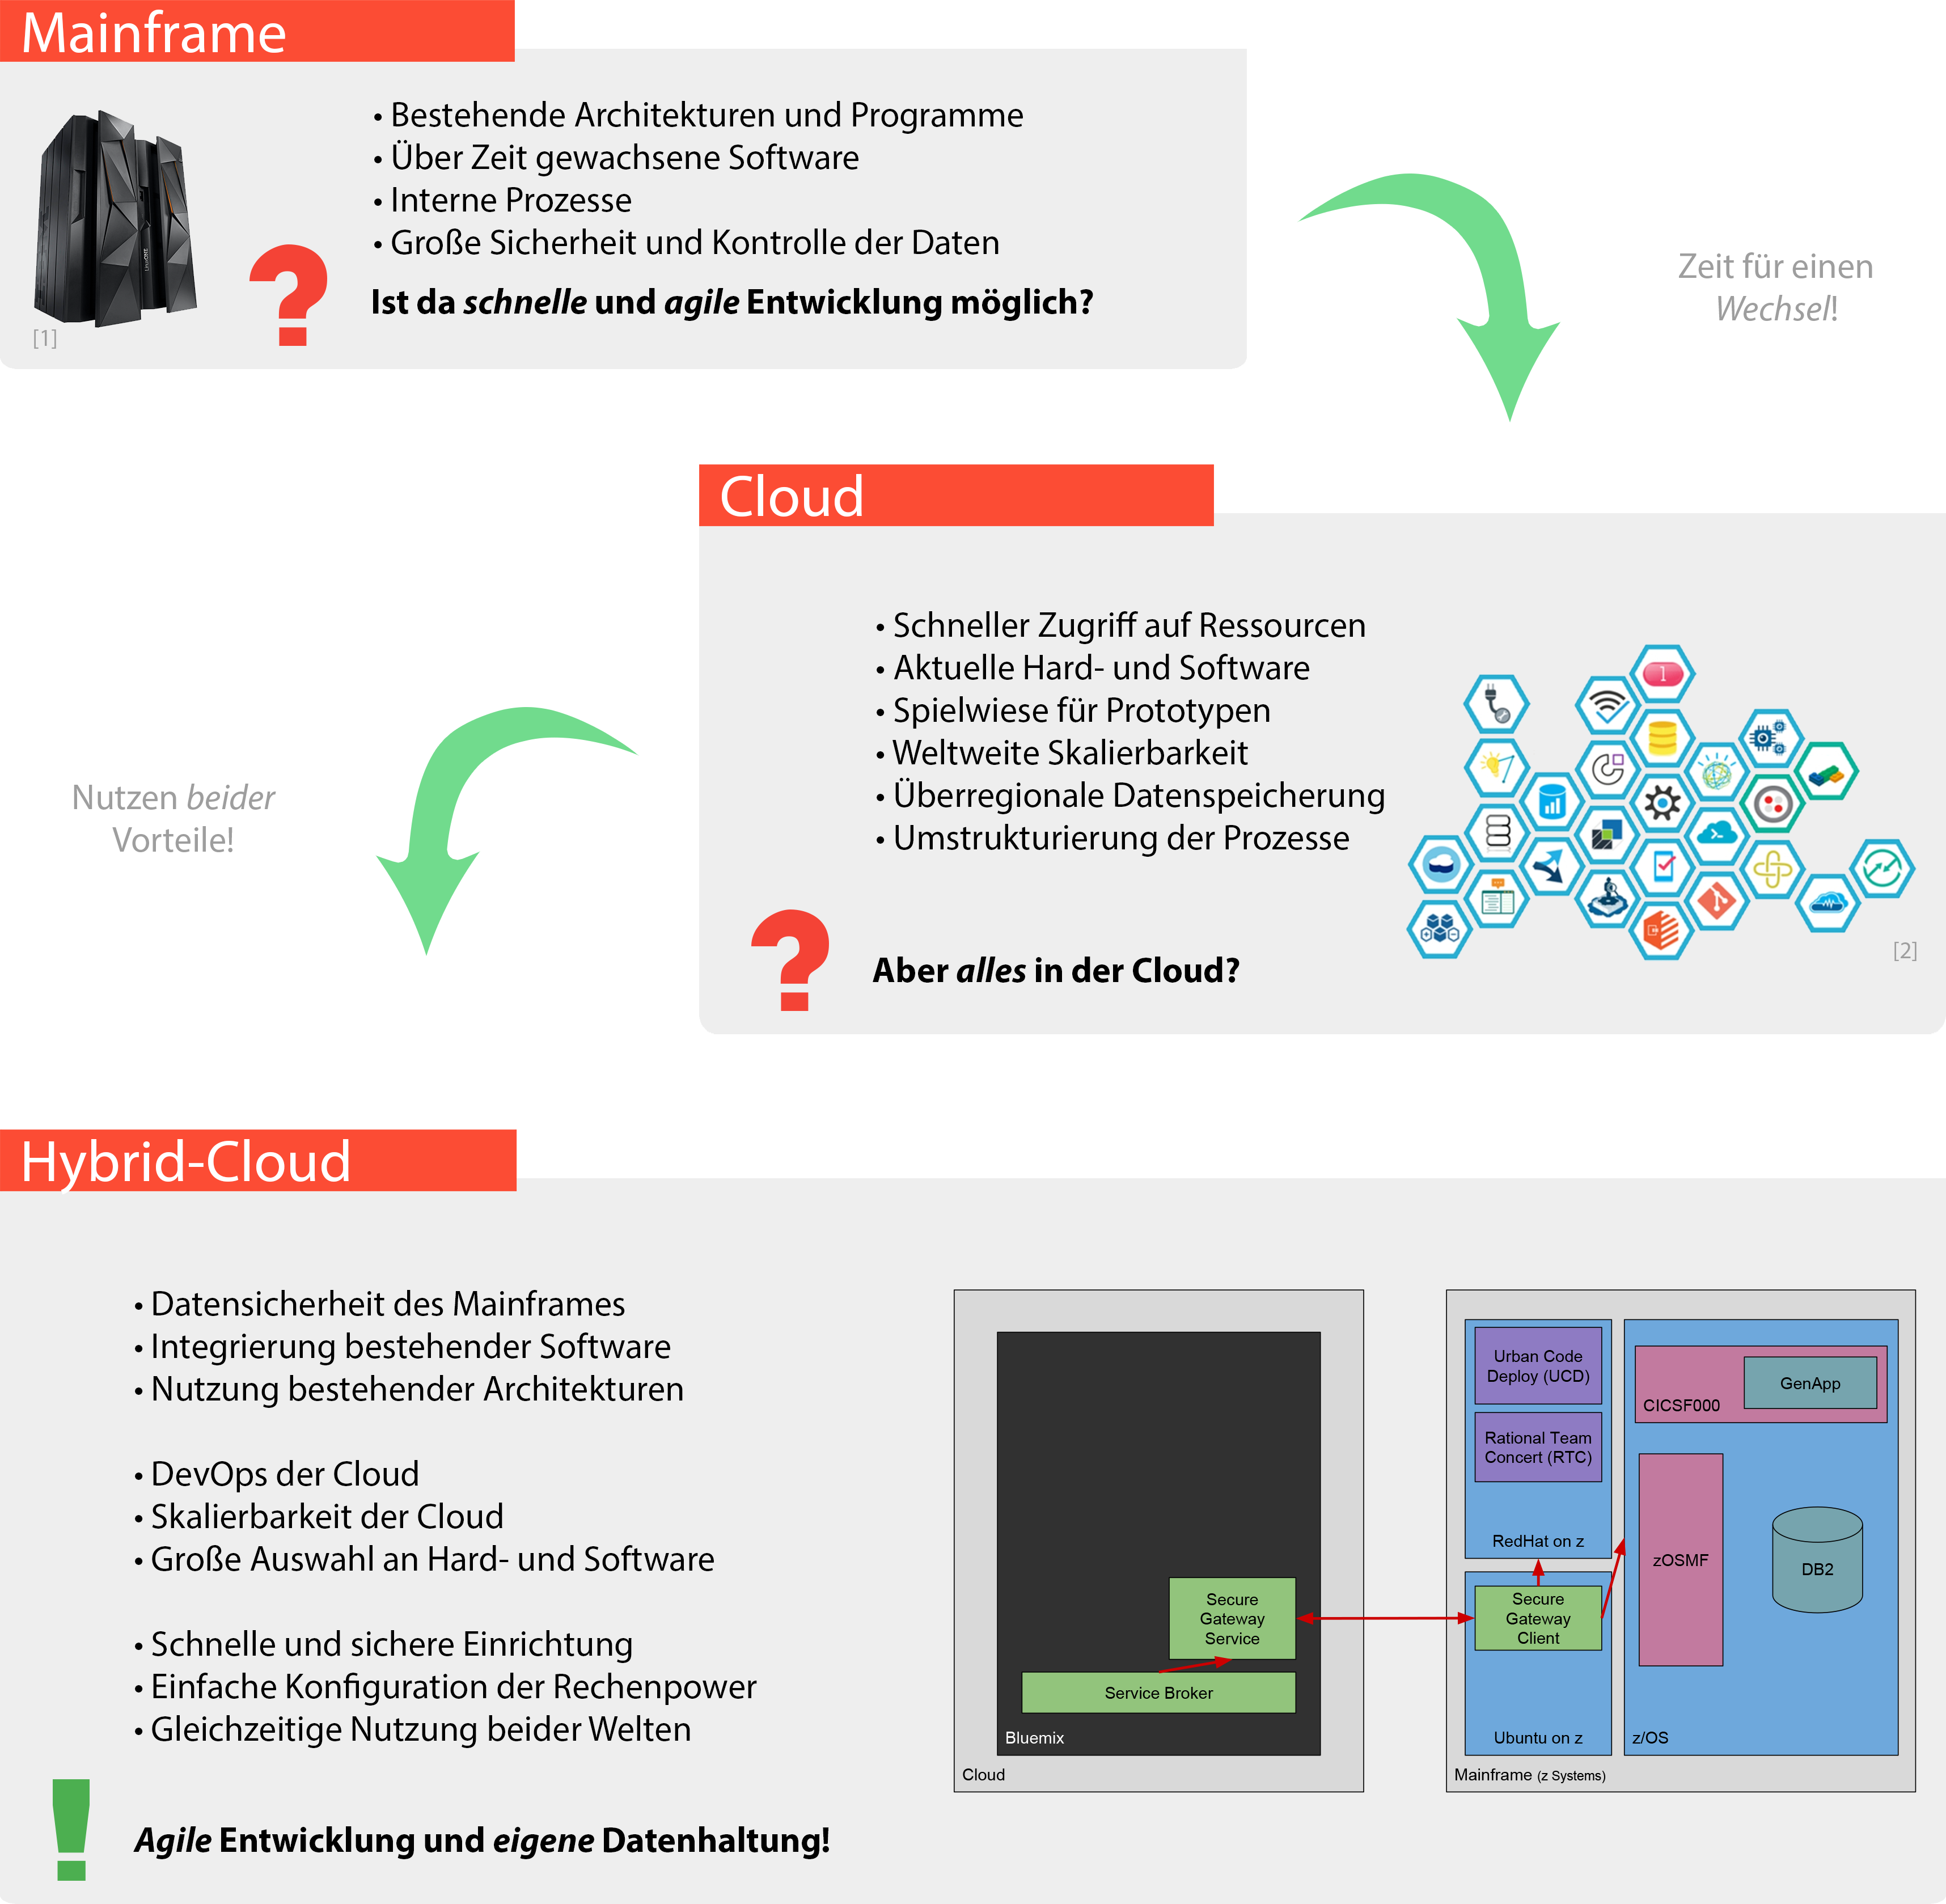
\includegraphics[scale=0.104]{images/kapitel_1/plakat.png}
  \caption{Entstehung der Hybrid-Cloud}
  \label{fig:plakat}
\end{figure}

\newpage

\section{Aufgabenstellung}
Das Kapitel soll eine kleine Übersicht über die Themen geben, welche in der Arbeit behandelt werden. Die Arbeit ist
in drei Themenbereiche unterteilt.

Der erste Teil der Arbeit befasst sich mit der Entwicklung einer Hybrid-Cloud-"-Architektur, welche die Cloud Infrastruktur
und die lokale Mainframe-Welt verbindet. Ein Unternehmen soll seine aufgebaute Mainframe-Umgebung weiter benutzen, aber
gleichzeitig die Vorteile der Cloud nutzen können.

Dazu zählen unter anderem die agilen Möglichkeiten bei der Entwicklung einer Anwendung (DevOps), höhere Geschwindigkeiten
bei der Freigabe neuer Releases und die einfache Verteilung der Applikationen über die ganze Welt ohne eigene Hardware
vorhalten zu müssen. Außerdem spielt die Skalierbarkeit und die Verfügbarkeit der eigenen Anwendung eine wichtige Rolle,
bei der die Cloud unterstützen kann.

Im zweiten Teil der Arbeit wird eine prototypische Anwendung entwickelt, welche die erstellte Architektur prototypisch
implementiert. Dabei soll die Architektur einer Machbarkeitsstudie unterzogen werden. Die Anwendung besteht aus einer
DB2 Instanz, einer COBOL-"-Runtime, einer COBOL-"-Anwendung, einem Java-"-Backend, einem Web-Frontend und zwei
Smartphone-"-Apps.

Der letzte Teil widmet sich dem Thema Qualitätssicherung in diesem Szenario. Fragen sind zum Beispiel, wie bei immer
schneller werdenden Releasezyklen die richtige Qualität der Anwendung gewahrt werden kann. Außerdem wird gezeigt, wie
die prototypische Anwendung aus dem zweiten Teil der Arbeit getestet werden kann.

Zum Schluss folgt ein Ausblick mit Anregungen und Ergänzungen sowohl für die Weiterentwicklung der Hybrid-Cloud-Architektur
als auch für das Web-Frontend und die Smartphone-Apps.

Ziel ist es, einem Unternehmen dabei zu helfen die Vorteile der Cloud und des Mainframes gemeinsam zu nutzen
ohne einen größeren Aufwand zu generieren. Außerdem soll aufgezeigt werden, wie bestehende Anwendungen als Services
für die Cloud bereit gestellt werden können.

\newpage

\section{Aufbau der Arbeit}
Dieses Kapitel dient zur schnellen Orientierung innerhalb der Arbeit und soll detaillierter zeigen, welche Themen in den
jeweiligen Kapiteln angesprochen werden.

\begin{description}

\item[Kapitel 2 (Grundlagen)]\hfill \\
In diesem Kapitel werden die Grundlagen erklärt. Es wird zum Beispiel der Unterschied einer Cloud zu einer Hybrid-Cloud
erläutert, um was es sich bei Bluemix handelt und was ein WebViewer ist.

\item[Kapitel 3 (Hybrid-Cloud-Architektur)]\hfill \\
Im dritten Kapitel wird eine Hybrid-Cloud-Architektur entwickelt und umgesetzt. Dabei werden verschiedene Optionen
für die einzelnen Teilaufgaben analysiert und im Anschluss die genutzten Programme installiert, eingerichtet und erläutert.
Anschließend wird die Architektur implementiert.

\item[Kapitel 4 (Prototypische Anwendung)]\hfill \\
Das vierte Kapitel setzt die Hybrid-Cloud-Architektur voraus und implementiert dazu eine prototypische Anwendung. Diese
besteht aus einem Backend, einem Frontend und zwei Smartphone-Apps. Dabei werden zu Anfang verschiedene Programme und
Services analysiert, um diese im Anschluss zu nutzen.

\item[Kapitel 5 (Qualitätssicherung)]\hfill \\
Dieses Kapitel beschäftigt sich mit dem Thema Qualitätssicherung und wie die Qualität bei immer schneller werdenen
Releasezyklen gewahrt werden kann. Dabei spielen automatische Tests eine wichtige Rolle.

\item[Kapitel 6 (Diskussion)]\hfill \\
Hier werden Themen angesprochen, die für die Verwendung der Hybrid-Cloud-\-Architektur erläutert werden müssen.
Unter anderem welche Rechte Entwickler in Zukunft haben sollen oder welche Use-Cases es für die Architektur gibt.

\item[Kapitel 7 (Ausblick)]\hfill \\
Wie sowohl die entwickelte Hybrid-\-Cloud-\-Architektur als auch die Anwendung erweitert werden können, wird in diesem
Kapitel aufgezeigt. Dabei können neue Cloud-Services hinzugefügt oder auch weitere Funktionen der schon eingesetzten
Services verwendet werden.

\item[Kapitel 8 (Zusammenfassung)]\hfill \\
Das letzte Kapitel enthält eine Zusammenfassung aller vorangegangenen Kapitel und ein Schlusswort.

\end{description}
\chapter{Grundlagen}
\label{cha:grundlagen}

Im folgenden Kapitel sollen die elementaren Grundlagen beschrieben werden, die zum Verständnis der nachfolgenden Kapitel
notwendig sind.

Der erste Abschnitt befasst sich mit der reinen Cloud und einer Abwandlung davon, der Hybrid-Cloud.

Der zweite Teil widmet sich den Produkten, die IBM in der Cloud und im Mainframebereich bietet. Dabei wird unter
anderem auf die Konfiguration der Produkte und Laufzeitumgebungen eingegangen wie auch Programme und Konzepte, welche in
der Arbeit benötigt werden, behandelt.

Im letzten Teil des Kapitels folgt die Beschreibung einer Designidee bei Smartphone-Apps und allgemeine Konzepte der
Softwareentwicklung.

\section{Cloud}
Der Begriff Cloud hat sich als Kurzform des Cloud Computing etabliert und versteht das Zusammenspiel von mehreren
Servern. Die Server übernehmen Aufgaben, wie etwa die Datenspeicherung oder komplizierte Programmabläufe. Dabei erkennt
der Cloud-Nutzer nicht, wie viele Server hinter der Cloud stecken oder wo diese sich befinden.

Selbst wenn ein Server ausfällt, hat dies keine Auswirkungen auf das gesamte System, da die Anfragen und Aufgaben auf
die anderen Systeme umgeleitet werden.

Die Cloud zeichnet sich nach NIST \cite{online_grundlagen_cloudNIST} und \cite{online_grundlagen_cloud} durch fünf
wesentliche Eigenschaften aus:

\begin{itemize}
    \item \textbf{On-Demand Self Service}   \\ Registrierte Nutzer können Resourcen selbstständig instantiieren und konfigurieren.
    \item \textbf{Broad Network Access}     \\ Der Zugriff kann von verschiedenen Endgeräten erfolgen.
    \item \textbf{Resource Pooling}         \\ Alle Resourcen des Anbieters werden gebündelt und nach Bedarf den Nutzern zugewiesen.
    \item \textbf{Rapid Elasticity}         \\ Kapazitäten können nach Bedarf skaliert werden und stehen schnell und dynamisch zur Verfügung.
    \item \textbf{Measured Service}         \\ Es existiert eine automatische Kontrolle der Ressourcen durch einen Zähler, welcher die Transparenz für den Anbieter und den Benutzer ermöglicht.
\end{itemize}

Neben vielen Cloud-Anbietern wie Amazon, SAP und Microsoft gibt es IBM mit \textbf{Bluemix}, welches im folgenden als Lösung für
die prototypische Implementierung dient.

\section{Hybrid-Cloud}
Mit Hybrid-Clouds werden Mischformen der public und der private Cloud bezeichnet. So laufen bestimmte Services bei
öffentlichen Anbietern über das Internet, während datenschutzkritische Anwendungen und Daten im Unternehmen betrieben
und verarbeitet werden. Die Herausforderung liegt hier in der Trennung der Geschäftsprozesse in datenschutzkritische
und -unkritische Workflows.

Voraussetzung ist eine saubere und konsequente Klassifizierung der im Unternehmen vorhandenen und verarbeiteten
Daten. Siehe dazu \cite{online_grundlagen_hybriddcloud}.

\section{Bluemix}
Bluemix ist die von IBM entwickelte Cloud-Platform. Über Bluemix greifen Entwickler auf mehr als 160 Cloud-Services zu,
um mobile Apps und Webanwendungen zu entwickeln. In Bluemix gibt es zahlreiche Analysewerkzeuge sowie Services von
Drittanbietern. Mit Watson Analytics lassen sich beispielsweise intelligente Systeme realisieren, die Daten
kognitiv (also selbstlernend, ohne für die Problemlösungen programmiert zu sein) auswerten und für die Entscheidungsfindung
aufbereiten.

Bluemix unterstützt diverse integrierte DevOps-Dienste, um Cloud-Anwendungen zu erstellen, auszuführen, bereitzustellen
und zu verwalten. Die Entwicklerplattform basiert auf der Technologie von Cloud Foundry und läuft auf IBMs
Softlayer-Cloud-Infrastruktur. Sie unterstützt mehrere Programmiersprachen, einschließlich Java, Node.js, Go, PHP, Python,
Ruby Sinatra, Ruby on Rails und kann auch andere Sprachen wie Scala durch den Einsatz von Buildpacks unterstützen
\cite{online_grundlagen_bluemix}.

Weitere Informationen über Bluemix können auf der Webseite\footnote{https://bluemix.net} gefunden werden.

\subsection{Public, Dedicated und Local}
Wie in \cite{online_grundlagen_bluemix_pdl} zu lesen, kann Bluemix in drei verschiedenen Varianten betrieben werden.

\begin{itemize}
    \item Bei \textbf{Public} werden Server, welche öffentlich im Internet zur Verfügung stehen, genutzt. Diese Variante wird gemeinhin als \path{Cloud} bezeichnet.
    \item Bei \textbf{Privat} können hingegen nur Server genutzt werden, die expliziet für den Kunden eingerichtet wurden.
    \item \textbf{Dedicated} ist ähnlich dem privaten Ansatz mit der Einschränkung, dass sich die Server im eigenen Rechenzentrum befinden.
\end{itemize}

Bei allen drei Formen wird das Management der Server sowie der Infrastruktur vollständig von IBM übernommen. Dies gilt
sowohl für die Wartung, das Einspielen von Updates und Funktionserweiterungen als auch für den Support.

Einige Services werden in den Bluemix Varianten \textit{Private} oder \textit{Dedicated} nicht angeboten und müssen über
die Cloud bezogen werden. Dies setzt eine Verbindung ins Internet voraus.

\subsection{Katalog}
Der Bluemix Katalog umfasst alle Software-as-a-Service (SaaS) und Platform-as-a-Service (Paas) Produkte, die sich der
Benutzer selbstständig instanziieren kann. Dabei werden die Produkte in drei größere Kategorien unterteilt.

Bei \textbf{Infrastruktur} werden entweder echte oder virtualisierte Ressourcen zur Verfügung gestellt. Zum Beispiel
handelt es sich dabei um \textit{vServer} oder ein \textit{z Systems}.

Desweiteren gibt es \textbf{Apps}, welche Docker-Contrainer, Cloud Foundry Runtimes oder OpenWhisk Trigger zur Verfügung
stellen.

Die letzte große Kategorie, \textbf{Service}, beinhaltet Funktionen, welche in eine Applikation eingebunden werden können.
Über diese Funktionen werden zum Beispiel Text2Speech Funktionen für eine Anwendung bereit gestellt.

\subsection{Cloud Foundry}
Cloud Foundry ist eine Open Source Platform as a service (PaaS) Lösung. Mit Hilfe von Cloud Foundry können Entwickler
ihre Anwendungen bauen, hochladen und ausführen. Ein großer Vorteil von Cloud Foundry ist die nahezu grenzenlose
Skalierbarkeit \cite{online_grundlagen_cloudfoundry}.

Die Skalierbarkeit wird durch die Container-Architektur erreicht. Jeder Container beinhaltet eine eigene Anwendungsinstanz.
Dabei wird sowohl eine horizontale als auch eine vertikale Skalierung unterstützt.

Bei der horizontalen Skalierung werden zusätzliche Container gestartet oder gestoppt und ein Load Balancer vor die Container
geschaltet. Bei der vertikalen Skalierung werden jeder Instanz individuell z.B. mehr oder weniger Arbeitsspeicher zugeteilt.

Jede Cloud Foundry Instanz besitzt eine IPV4-Adresse wodurch es mittels A-Record (Zuordnung eines DNS-Namens zu IP-Adresse)
möglich ist, eine eigene Domain mit der Anwendung zu verknüpfen.

\section{Services}
In Bluemix gibt es mehr als 160 Funktionen. Eine großer Bereich sind die Services, welche eine
der drei Kategorien darstellt. Mit den Services können Applikationen durch vorgefertigte Funktionen erweitert werden.
Eine Bilderkennung oder Text in Sprache umwandeln sind nur wenige Beispiele.

\subsection{Secure Gateway}
Mit dem Secure Gateway können verschiedene Netzwerke miteinander verbunden werden. Dazu wird eine sichere Verbindung
zwischen Bluemix und einem anderen Netzwerk aufgebaut. Dies kann lokal im eigenen Rechenzentrum liegen oder in einer
anderen Cloud. Siehe dazu auch \cite{online_grundlagen_securegateway}.

Zur Verbindung wird ein Client im Zielnetzwerk installiert und anschließend eingerichtet.

Ein wesentlicher Vorteil des Secure Gateways ist, dass sich der installierte Client auf den Bluemix-Service verbindet und
nicht umgekehrt. Dies erleichtert die Konfiguration innerhalb des Unternehmensnetzwerkes, da z.B. keine feste IP-Adresse
vorausgesetzt wird.

\subsection{Service Broker}
Durch einen Service Broker können Cloudanwendungen geschrieben werden, welche bestehende Services erweitern oder
zusätzliche hinzufügen. Jeder Service in Bluemix besteht aus einem Service Broker.

Die Cloud Foundry Foundation hat einen offenen Standart für Schnittstellen definiert, welcher von allen größeren
Cloud-Anbietern eingehalten wird. Diesem \textit{Open Service Broker API} Projekt gehören diverse Firmen an. Mehr dazu
unter \cite{online_grundlagen_servicebrokerapi}.

Die Einrichtung eines Service Brokers in den eigenen Katalog erfolgt durch das Hinzufügen des Services in einen der zwei
zur Verfügung stehenden Scopes (Siehe dazu \cite{online_grundlagen_servicebroker}).

\subsection{Scopes}
\label{sub:scopes}
In Bluemix stehen zwei verschiedene Scopes (Bereiche) für einen Service Broker zur Verfügung.

Im \textbf{Standard Broker} kann der Service Broker für alle Endkunden oder nur für einzelne Benutzergruppen bereitgestellt
werden. In diesen Scope kann in der Regel nur der Administrator Service Broker hinzufügen.

Im \textbf{Space-Scoped Broker} steht der Service Broker nur für Mitglieder der gleichen Organisation zur Verfügung. In
diesen Scope kann jeder Benutzer einen eigenen Service Broker installieren und freigeben
(Siehe auch \cite{online_grundlagen_servicebroker_scope}).

\subsection{Toolchain}
Bei einer Toolchain handelt es sich um ein Tool zur Verwaltung von Entwicklung, Bereitstellung sowie Überwachung einer
Anwendung. Nach der Einrichtung einer Toolchain stehen verschiedene Services zur Verfügung, welche zum Beispiel eine Integration
zu einem GitHub-Projekt ermöglichen.

Mit einer eingerichteten Toolchain und einem verbundenen Git-Repository kann der Quelltext gebaut und auf einem System
installiert werden. Bei der Toolchain handelt es sich unter anderem um ein \textit{Continuous Integration}-Tool (kurz CI)
(Mehr unter \cite{online_grundlagen_toolchain}).

\section{Mainframe}
Mainframes bezeichnen leistungsfähige Großrechner, die in Rechenzentren installiert sind. Sie werden meist als
Hintergrundrechner eingesetzt, wo sie zum Beispiel für die Massendatenverarbeitung zuständig sind.

Mainframes sind immer dann sinnvoll, wenn eine Anwendung auf einem anderen Computer nicht lösbar ist oder wenn das Abarbeiten
der Anwendung auf einem herkömmlichen Computer viel zu lange dauern würde (Siehe hierzu auch \cite{book_grundlagen_mainframe}).

Die Einrichtung und Wartung eines Mainframes bedarf eines Grundverständnisses des Betriebssystems und dessen Architektur.

Neben anderen Herstellern von Mainframes gibt es IBM mit \textbf{z Systems}, welches im Folgenden näher betrachtet wird.

\subsection{z Systems}
IBM z Systems ist der Name für alle Mainframes von IBM. Der Name wurde offiziell im April 2006 veröffentlicht und von da an
ausschließlich genutzt. Vor allem durch die 64-Bit-Architektur zeichnet sich z Systems vom Vorgänger s/390 aus. Allerdings
werden ältere Programme, die noch nicht für 64-Bit angepasst wurden, ebenfalls unterstützt (Mehr in \cite{book_grundlagen_zsystems}).

\subsection{zOSMF}
IBM z/OS Management Facility (kurz zOSMF) vereinfacht die Konfiguration und unterstützt bei Managementaufgaben in einer
z/OS Umgebung. Es bietet zahlreiche optimierte Prozesse für Verwaltungsaktivitäten. Außerdem hilft es bei wiederholbaren
Aufgaben, diese zu erleichtern und zu automatisieren.

Bei zOSMF handelt es sich um eine Weboberfläche, die vom Netzwerk des Mainframes aus aufgerufen werden kann. Ein weiterer
großer Vorteil des Konfigurationsprogramms ist die REST-Schnittstelle, die es zur Verfügung stellt (Mehr über zOSMF unter
\cite{online_grundlagen_zosmf}).

Weitere Informationen und Anleitungen sind auf der zOSMF-Webseite\footnote{https://www-03.ibm.com/systems/z/os/zos/features/zosmf}
zu finden.

\subsection{CICS}
Bei Customer Information Control System (kurz CICS) handelt es sich um ein von IBM entwickeltes Programm für die
Online-Transaktionsverwaltung. Es hat sich, zusammen mit der Programmiersprache COBOL, als das weitverbreitetste Toolset
für Kundentransaktionsanwendungen im Bereich des Mainframe-Computings etabliert. Bei den meisten Legacy-Anwendungen handelt
es sich um COBOL/CICS-Programme.

Mit der API, welche CICS bereitstellt, kann ein Entwickler Anwendungen schreiben, welche mit Online-Usern kommunizieren
und Datensätze aus einer Datenbank auslesen und schreiben. Dabei werden nicht IBM-Methoden sondern CICS-Funktionen
gennutzt.

Wie andere Transaktionsmanager kann CICS sicherstellen, dass eine Transaktion korrekt abgeschlossen wurde. Falls Probleme
auftreten ist das System selbstständig in der Lage, Transaktionen rückgängig zu machen. Die Integrität von
Datensätzen bleibt dabei stets erhalten (Siehe mehr in \cite{book_grundlagen_cics} und \cite{online_grundlagen_cics}).

\section{DB2}
Bei DataBase 2 (DB2) handelt es sich um ein relationales Datenbankmanagementsystem von IBM \cite{book_grundlagen_db2}.
Seit Version 11 wird ein REST-Interface Service unterstützt, durch den eigene Schnittstellen definiert und aufgerufen
werden können.

\section{UrbanCode Deploy}
UrbanCode Deploy (kurz UCD) ist ein Tool für die Automatisierung der Anwendungsbereitstellung, das ein schnelles Feedback
und die Continuous Delivery in einer agilen Entwicklung vereinfachen und gleichzeitig die erforderlichen Versionskontrollen
und Genehmigungen für Produktionsumgebungen bereistellt.

Durch die Verwendung von UCD in Verbindung mit IBM Bluemix Private Cloud können Entwickler die Anwendungsbereitstellung
und das Management in mehreren Cloudumgebungen und Anwendungen beschleunigen.

\section{Rational Team Concert}
Bei IBM Rational Team Concert (kurz RTC) handelt es sich um eine kollaborative Lösung für das Life-Cycle-Management von
Softwareanwendungen, die auf der offenen IBM Technologieplattform Jazz basiert. Das Produkt bietet grundlegende
Projektplanung, Work Item Management, Software-Versionierung, Arbeitsbereichsverwaltung und die Unterstützung paralleler
Entwicklung.

Außerdem wurde RTC dafür ausgelegt, verteilte Entwicklungsteams zu verbinden, die Produktivität jedes Einzelnen sowie des
Teams zu steigern, die Entwicklungszyklen zu verkürzen und in kürzester Zeit qualitativ hochwertige Software bereitzustellen.

\section{WebView}
Bei WebView handelt es sich um ein Android- und iOS-Layout, das Webseiten darstellen kann. Über Schnitstellen werden
Informationen wie Webseite, URL und Größe übergeben. Das Laden, das Anzeigen und die Interaktion mit der Webseite übernimmt
das Layout selbstständig.

Das Layout steht sowohl unter Android als auch iOS in den frühesten Versionen zur Verfügung (Weitere Informationen unter
\cite{online_grundlagen_webviewer}).

\section{Serviceorientierte Architektur}
Hinter SOA, also den serviceorientierten Architekturen, steckt die Idee, die Programmlogik auf verschiedene
Services zu verteilen und sie nicht in einem einzelnen Programm zu bündeln. Prozesse werden so als eigenständige Services
definiert.

Funktionen, die durch einzelne Systeme abgedeckt werden, sind dank SOA in standardisierter Form unternehmensweit
zugänglich. Einmal erstellte Funktionen können also immer wieder verwendet werden (\cite{book_grundlagen_soa}).

Anwendungen greifen über die HTTP-Methoden wie zum Beispiel \textit{GET}, \textit{POST}, \textit{PUT}, \textit{PATCH}
und \textit{DELETE} auf die REST-Schnittstellen der Services zu und kommunizieren über \textit{JSON} oder \textit{XML}
Objekte.

\section{Model-View-Controller}
Model-View-Controller (kurz MVC) wurde um 1978 von Xerox entwickelt und es handelt sich dabei um eine Architektur von
Programmen.

In MVC wird eine Anwendungskomponente in drei Teile zerlegt. In das oberflächenunabhängige \textit{Model}, das für die
Ausgabe zuständige \textit{View} und den für die Interpretation von Eingabeereignissen zuständigen \textit{Controller}.

Der Controller ist die Steuerungseinheit, das Model der Anwendungskern und die View der Darsteller bzw. die Ansicht der
Anwendung. Ein View zusammen mit seinem Controller wird hier auch als eine Oberfläche bezeichnet.
(Mehr hierzu unter \cite{book_prototypischeanwendung_mvc})

Es gibt zahlreiche Frameworks, welche das MVC-Patern umsetzen. AngularJS ist einer der bekanntesten Vertreter.

\section{REST}
REST-API steht für Representational State Transfer - Application Programming Interface. Diese Interfaces machen den
Austausch von Informationen über unterschiedliche Systeme möglich. Im Zeitalter verteilter Systeme und Cloud-Computing
trifft man oft auf unterschiedliche Systeme, welche den Einsatz von REST-API notwendig machen.

Man spricht bei REST-API auch von der Maschine-Maschine-Kommunikation, da die verschiedenen Systeme
und Geräte zusammengebracht werden und gewissermaßen die gleiche Sprache sprechen.

Mit REST-API ist es möglich geworden, Informationen und Aufgaben auf verschiedene Systeme zu verteilen und diese mit der
Hilfe von HTTP-Requests anzufordern. Jeder HTTP-Request setzt sich aus dem Endpoint und den entsprechenden Parametern
zusammen \cite{online_grundlagen_rest}.

\chapter{Hybrid-Cloud-Architektur}
\label{cha:hybrid_cloud_architektur}

Im folgenden Kapitel wird eine Hybrid-Cloud-Architektur entwickelt. Dafür wird, wie in Abbildung
\ref{fig:architektur_uebersicht} auf Seite \pageref{fig:architektur_uebersicht} zu sehen, eine dauerhafte Verbindung
zwischen dem Netzwerk der Cloud-Infrastruktur und dem lokalen Netzwerk des Mainframes hergestellt. Diese Verindung soll
über mehrere Kommunikationskanäle verfügen, um verschiedene Programme miteinander zu verbinden.

Anschließend soll es in der Cloud eine Konfigurationsansicht geben um Ressourcen auf dem Mainframe zu verwalten. Dazu
gehört neben dem Erstellen dieser auch das Starten, Stoppen und Löschen. Die Ansicht soll außerdem Informationen über
die einzelnen Ressourcen und das Gesamtsystem anzeigen und auswerten können.

Des Weiteren wird eine Möglichkeit gefunden, wie Quellcode, welcher entweder in der Cloud oder in einem lokalen RTC
gespeichert ist, gebaut und in der Cloud oder auf dem Mainframe installiert und ausgeführt werden kann.

Einem Entwickler soll es in Zukunft möglich sein, seinen Quellcode lokal auf einem Mainframe oder in einer Cloud zu
verwalten, anschließend Ressourcen sowohl in der Cloud als auch auf dem Mainframe bereitzustellen, seinen Quellcode zu
bauen und auf beiden Systemen einzurichten.

Auch soll es dem Entwickler möglich sein, ein Segment seiner Anwendung auf dem lokalen Mainframe und das andere in der
Cloud bereitzustellen. Somit können bestehende Anwendungen weiterhin genutzt werden. Eine Kommunikation der beiden
Segmente vorausgesetzt.

\begin{figure}[h]
  \centering
    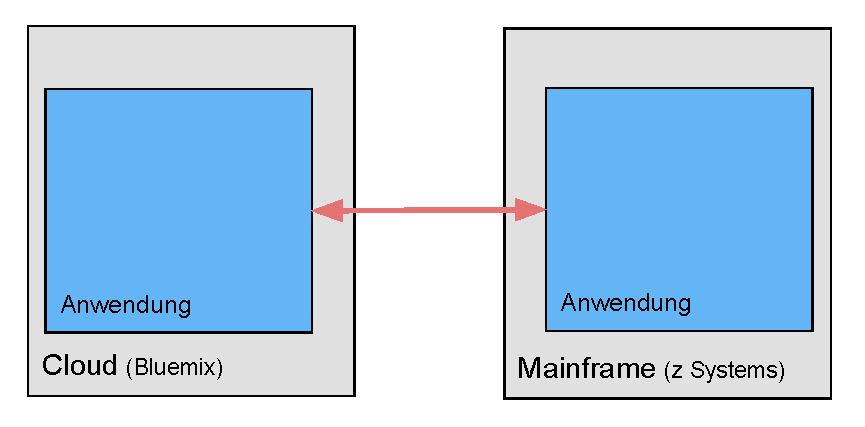
\includegraphics[scale=0.5]{images/kapitel_3/architektur_uebersicht.pdf}
  \caption{Schematische Darstellung der Hybrid-Cloud-Architektur}
  \label{fig:architektur_uebersicht}
\end{figure}
\section{Analyse}

\subsection{Aufgaben}
Um auf dem Mainframe verschiedene Aufgaben durchzuführen, gibt es mehrere Möglichkeiten. Eine ist das Ausführen von Kommandos
über ein Terminal. Eine andere, das Schreiben von eigenen Shell-Scripten, welche diese Aufgaben erledigen.

Alternativ können alle Aufgaben mit dem in z/OS-Version 1.13 eingeführten zOSMF durchgeführt werden. Dabei handelt es
sich um ein Web-Interface, mit dem zahlreiche Konfigurationen auf dem Mainframe vorgenommen werden können. Das Interface
besitzt darüber hinaus eine RESTFul-Schnittstelle, die es ermöglicht, eigene Programme für einzelne Aufgaben zu schreiben,
die bequem gesteuert werden können.

Ein Vorteil dabei ist, dass die geschriebenen Programme, welche die RESTFul-Schnit\-tstelle von zOSMF ansteuern, nicht auf
dem gleichen System bereit stehen müssen. Sie müssen lediglich eine Verbindung bzw. einen Kommunikationskanal zum zOSMF
haben.

\subsection{Konfigurationsinterface}
Um Ressourcen auf einem Mainframe bereit zu stellen, wird ein Interface zur Verwaltung benötigt. In dieser Arbeit stehen
zwei mögliche Interfaces zur Auswahl. Das lokale zOSMF und Bluemix, die von IBM
veröffentlichte Plattform für Cloud-Anwendungen.

Mit dem Interface soll es möglich sein, neue Ressourcen zu provisionieren, zu starten, zu stoppen und zu löschen. Außerdem
soll das Interface Informationen über die vorliegende Konfiguration und Ressourcen anzeigen können. Des Weiteren soll es
definierte Workflows in UCD starten und stoppen können.

Die Wahl fiel zugunsten von Bluemix aus, da dies öffentlich im Internet zur Verfügung steht, wohingegen zOSMF ggf. eine
VPN-Verbindung ins Netz des Mainframes voraussetzt. Außerdem enthält Bluemix, im Gegensatz zu zOSMF, die Cloud Services.

\subsection{Kommunikation}
Damit von Bluemix aus die RESTFul-Schnittstelle sowohl von zOSMF als auch von UCD angesteuert werden kann, muss eine
dauerhafte Verbindung zwischen Cloud und lokalem Netzwerk des Mainframes hergestellt werden. Dazu ist es nötig eine
VPN-"-Verbindung zwischen den beiden Netzwerken aufzubauen. Diese kann entweder manuell eingerichtet, gewartet und
gesichert werden, oder es wird der Secure Gateway Service von Bluemix genutzt.

Da sich der Secure Gateway Service selbst um die Verbindung und Authentifizierung zwischen Client und Server kümmert, wird
dieser in der Architektur genutzt. Ein weiterer Vorteil ist die leichte Konfiguration und die automatische Wiederverbindung
nach einem Neustart des Systems oder einem Verbindungsabbruch.

Außerdem können durch den Service mehrere Verbindung zwischen Cloud und Mainframe hergestellt werden, welche durch
unterschiedliche Ports realisiert werden.

\subsection{Verteilte Versionskontrolle}
Für das Speichern und Verwalten von Quelltext kommen mehrere Services in Frage. Einerseits die in Bluemix zur Verfügung
gestellten Services zur Integration von GitHub oder ein selbst gehostetes Git-Repository, alternativ auch
ein RTC, welches auf einem Mainframe installiert werden kann.

Für die Architektur ist es sinnvoll, beide Möglichkeiten zu unterstützen. So ist es möglich, den Quelltext in der Cloud
auf einem GitHub-Repository zu verwalten oder mittels RTC, lokal auf dem Mainframe.

Ein weiterer Vorteil bei der Unterstützung beider Möglichkeiten ist, dass sowohl der Quelltext, welcher in einem Cloud-Repository
verwaltet wird, durch ein Deployment auf einem lokalen Mainframe installiert, als auch der lokale Quelltext im
RTC in einer Cloud-Umgebung installiert werden kann.

\subsection{Continuous integration}
Für einen kontinuierlichen Bau eines Artefaktes aus dem Quelltext gibt es im Aufbau zwei Möglichkeiten. Entweder
den Toolchain-Service in Bluemix oder das UCD, lokal auf dem Mainframe.

Da es schon eine Verbindung zu UCD gibt und der Quelltext entweder lokal oder in der Cloud abgelegt werden kann,
werden beide Möglichkeiten umgesetzt.

So ist es möglich, mittels einer Bluemix Toolchain und verbundenem Git-Repository
das Artefakt in einer CICS-Region von der Cloud aus zu installieren oder durch das UCD, welches den Quellcode von einem RTC
lokal auf dem Mainframe abgreift.

\subsection{Qualitätssicherung}
Damit bei einem regelmäßigen Bau des Quellcodes nach einem Git-Commit die richtige Qualität gewahrt werden kann, müssen
automatisierte Tests hinterlegt werden.

Da sowohl die Bluemix Toolchain als auch UCD in der Architektur eingesetzt werden, wird in beiden Deployment-Scripten
ein Block hinzugefügt, welcher die Tests ausführt, die für die jeweilige Anwendung geschrieben wurden.
\section{Vorbereitung}
In diesem Abschnitt werden Vorbereitungen für die Entwicklung mit und auf Bluemix getroffen. Dabei werden unter anderem
Programme auf dem Entwicklungscomputer installiert und eingerichtet. Diese Schritte werden benötigt, da sonst nicht mit
den Systemen gearbeitet werden kann.

\subsection{Bluemix Konto}
Um mit Bluemix arbeiten zu können, wird ein kostenloses Benutzerkonto vorausgesetzt. Dieses kann über die
Registrierungs-Seite\footnote{https://console.ng.bluemix.net/registration} angelegt werden.

Ab dem Zeitpunkt der Registrierung erhält der Benutzer 30 Tage alle Services komplett kostenlos.

Nach dem erfolgreichen Anlegen des Benutzerkontos wird nach einem Namen für den ersten Bereich gefragt. Die Benamung des
Bereichs spielt dabei keine Rolle und kann frei gewählt werden. Ein Beispiel hierfür wäre \path{Hybrid Cloud}.

\subsection{Cloud Foundry CLI}
Für die weitere Konfiguration von Bluemix wird das Command Line Interface (kurz CLI) von Cloud Foundry genutzt (auch
Cloud Foundry CLI oder kurz CF genannt). Die Installation erfolgt unter Ubuntu mittels der folgenden Kommandos.

\begin{lstlisting}[language=bash, caption=Installieren der Cloud Foundry CLI, label=Installieren der Cloud Foundry CLI]
   $ wget -q -O - https://packages.cloudfoundry.org/debian/cli.cloudfoundry.org.key | sudo apt-key add -
   $ echo "deb http://packages.cloudfoundry.org/debian stable main" | sudo tee /etc/apt/sources.list.d/cloudfoundry-cli.list
   $ sudo apt-get update
   $ sudo apt-get install cf-cli
\end{lstlisting}

Ein Installer für Windows und MacOS steht im öffentlichen GitHub-Repository\footnote{https://github.com/cloudfoundry/cli}
von Cloud Foundry zur Verfügung.

Anschließend kann im Terminal, um die Installation zu überprüfen, die Version der Cloud Foundry CLI abgefragt werden. Dies
geschieht über den Parameter \path{version}.

\begin{lstlisting}[language=bash, caption=Version der Cloud Foundry CLI überprüfen, label=Version der Cloud Foundry CLI überprüfen]
   $ cf --version
\end{lstlisting}

Es sollte eine Version größer \path{6.x} angezeigt werden. Zum Beispiel \path{cf version 6.22.2+a95e24c-2016-10-27}.

Eine Übersicht über die wichtigsten Befehle der Cloud Foundry CLI ist auf der Bluemix
Hilfeseite\footnote{https://console.ng.bluemix.net/docs/cli/reference/cfcommands/index.html} zu finden.
\section{Umsetzung}
Wie auf dem Zielarchitekturbild in Abbildung \ref{fig:architektur_gesamt} auf Seite \pageref{fig:architektur_gesamt}
zu sehen, befinden sich insgesamt drei virtuelle Maschinen auf dem Mainframe. Ein Ubuntu-, ein RedHat- und ein
z/OS-System. Alle drei Systeme befinden sich im gleichen Netzwerk und teilen sich die gleiche Hardware.

Auf dem Ubuntu System ist der \textit{Secure Gateway Client} (kurz SGC) installiert, welcher eine Verbindung mit dem
zugehörigen Bluemix Service aufbaut.

Das RedHat System hat das \textit{UrbanCode Deploy} (kurz UCD), sowie das \textit{Rational Team Concert} (kurz RTC)
installiert. Mit diesen Tools ist das Speichern, Verwalten und Bauen von Quellcode möglich.

Auf der z/OS Maschine ist neben dem \textit{zOSMF} auch eine \textit{DB2} Instanz installiert. Außerdem ist eine
CICS-Runtime eingerichtet, welche mehrere CICS-Regionen verwalten kann. Die CICS-Regionen können entweder leer oder mit
einer beliebigen Applikation eingerichtet werden.

In Bluemix ist neben dem schon beschriebenen \textit{Secure Gateway}-Service der \textit{Service Broker} instanziiert.
Der Service Broker ist die Konfigurationsansicht und Verwaltung der Hybrid-Cloud und übernimmt die Kommunikation zwischen
Bluemix und zOSMF bzw. UCD.


\begin{figure}[h]
  \centering
    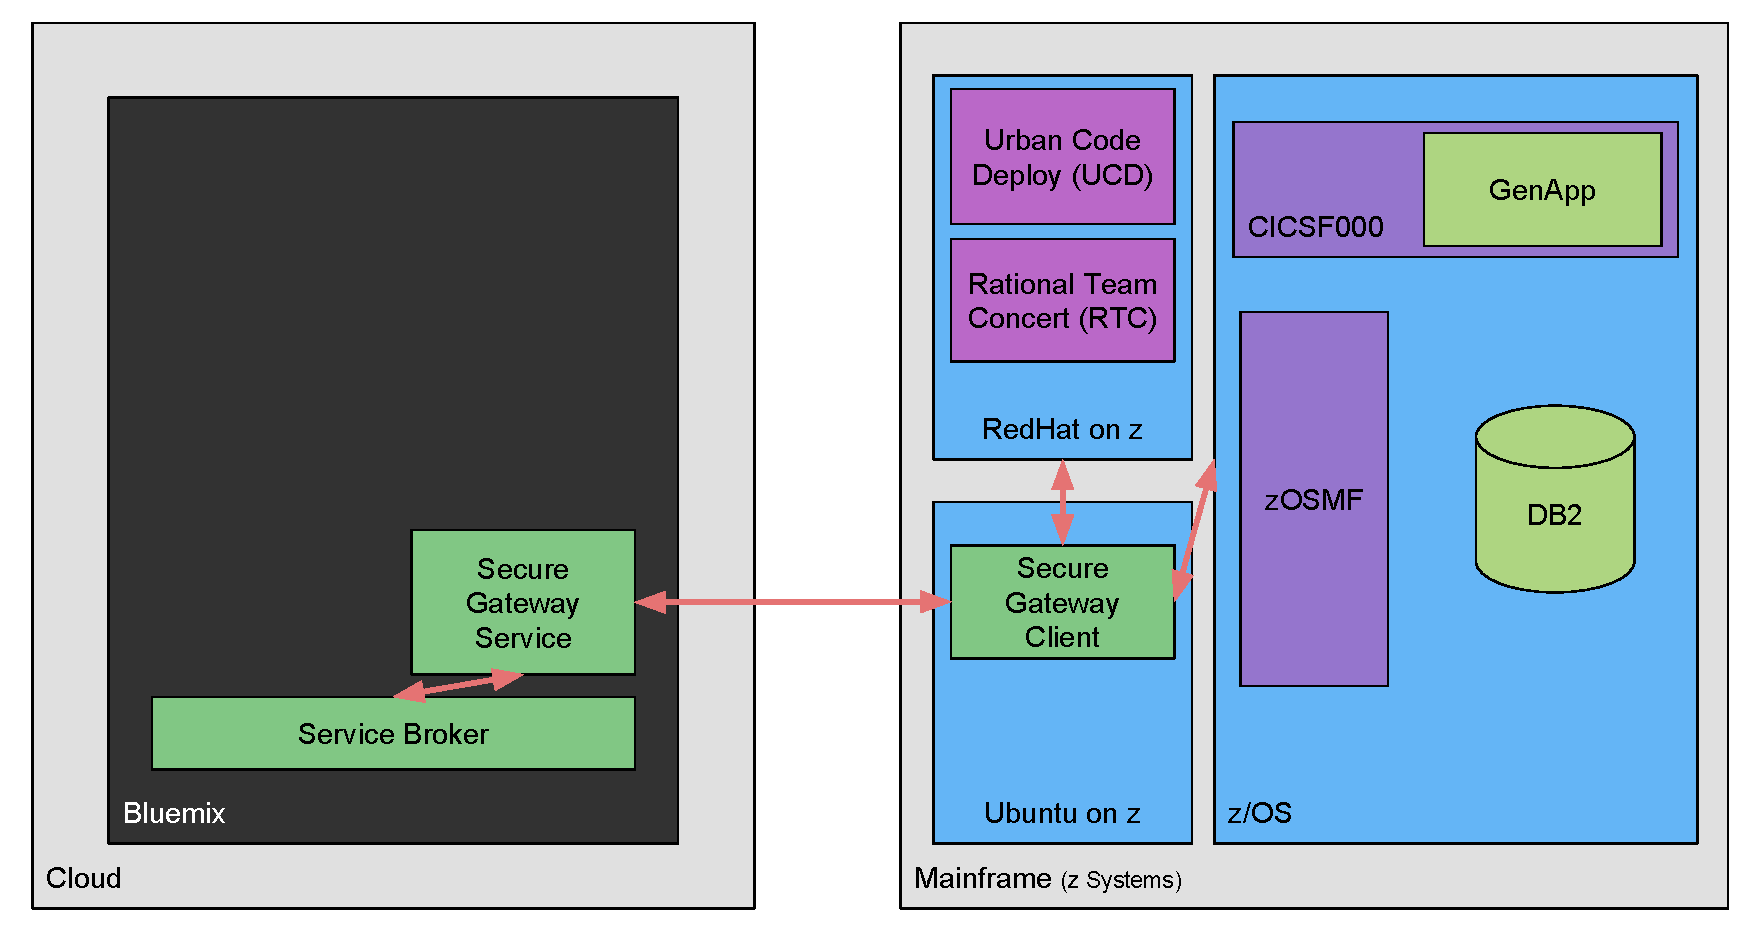
\includegraphics[scale=0.48]{images/kapitel_3/architektur_gesamt.pdf}
  \caption{Übersicht der Zielarchitektur}
  \label{fig:architektur_gesamt}
\end{figure}

\subsection{Erstellen eines Software Service Templates}
Damit CICS-Regionen automatisiert auf dem Mainframe erstellt werden können, muss ein Software Service Template (auch
Workflow genannt) in zOSMF angelegt werden. Dies kann anschließend wiederholt gestartet werden.

Um einen Workflow anzulegen wird das zOSMF in einem Webbrowser geöffnet und nach einem erfolgreichen Login erscheint auf der
linken Seite das Konfigurationsmenü (siehe dazu Abbildung \ref{fig:zosmf_uebersicht} auf Seite \pageref{fig:zosmf_uebersicht}).

\begin{figure}[h]
  \centering
    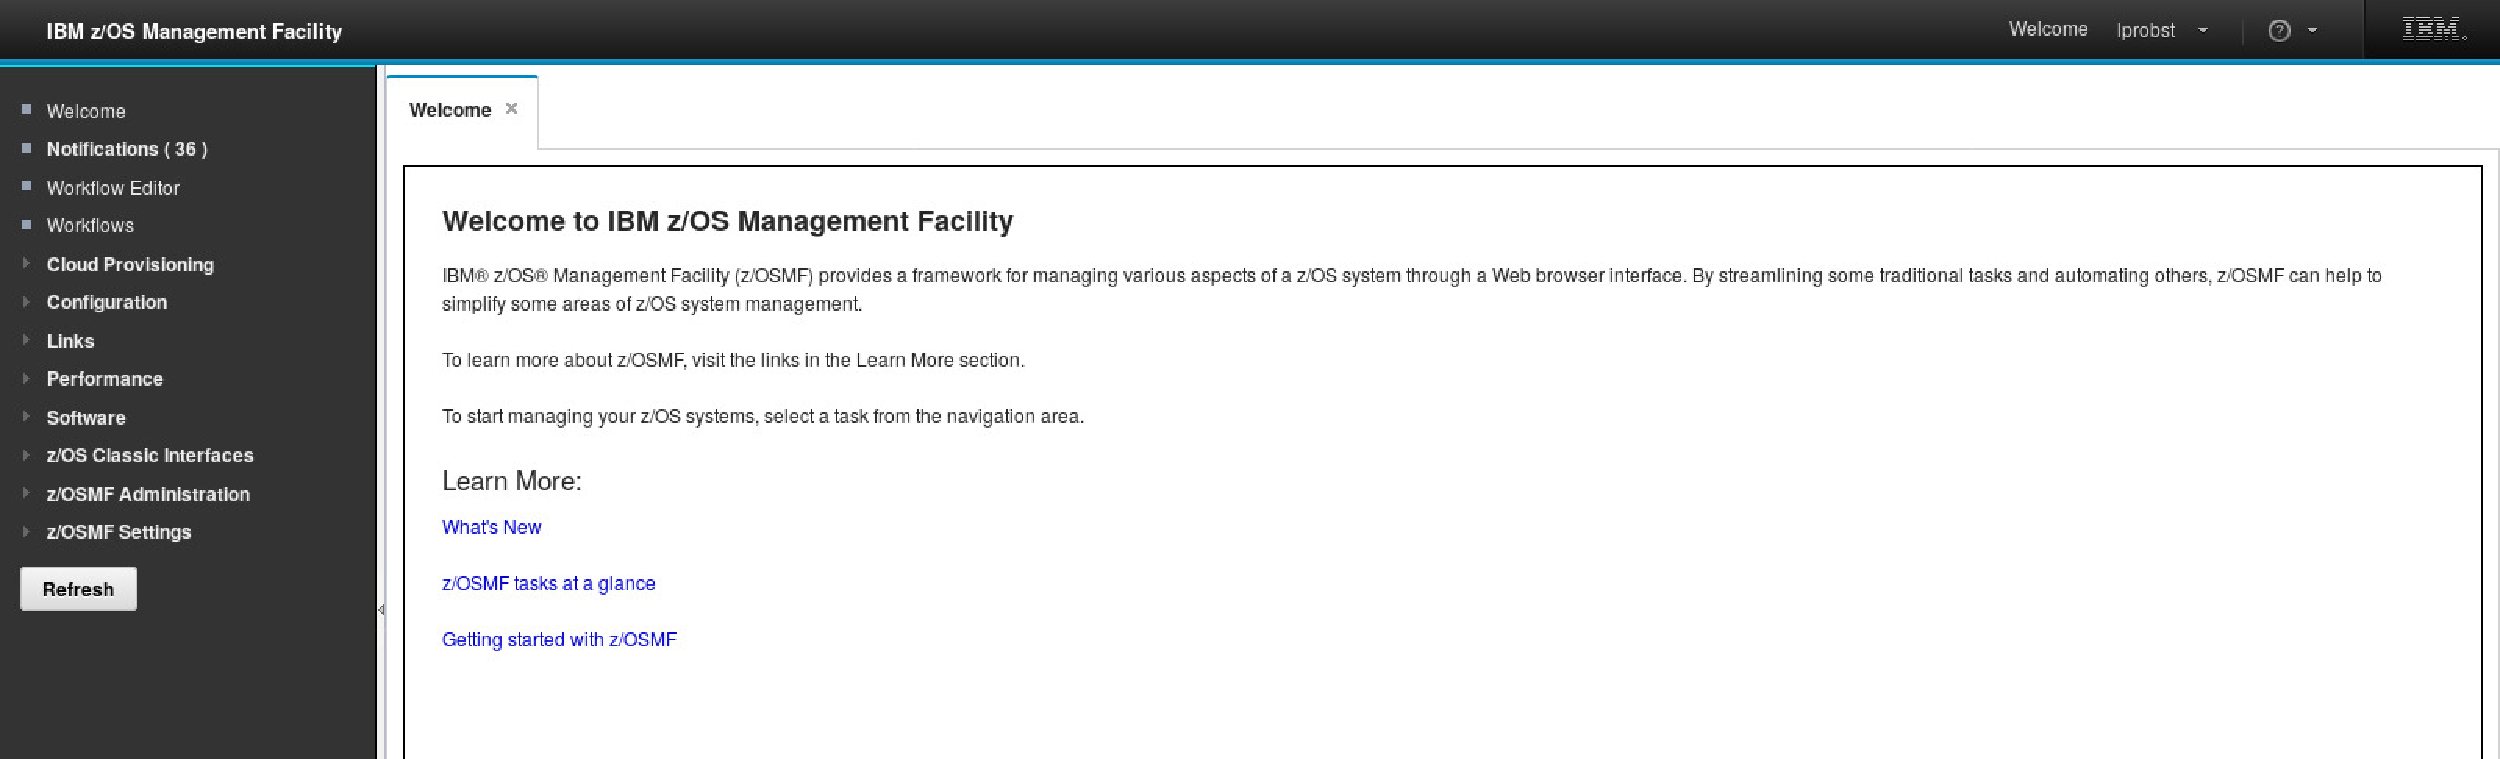
\includegraphics[scale=0.32]{images/kapitel_3/zosmf_uebersicht.pdf}
  \caption{Web-Interface von zOSMF}
  \label{fig:zosmf_uebersicht}
\end{figure}

Dort kann über den Menüpunkt \path{Cloud Provisioning} und anschließendem Klick auf \path{Software Service} die Übersicht
der CICS-Regionen angezeigt werden. Wie in Abbildung \ref{fig:zosmfsoftwareservice} auf Seite
\pageref{fig:zosmfsoftwareservice} zu sehen sind in diesem Beispiel derzeit sechs CICS-Regionen eingerichtet und drei
wurden gelöscht.

\begin{figure}[h]
  \centering
    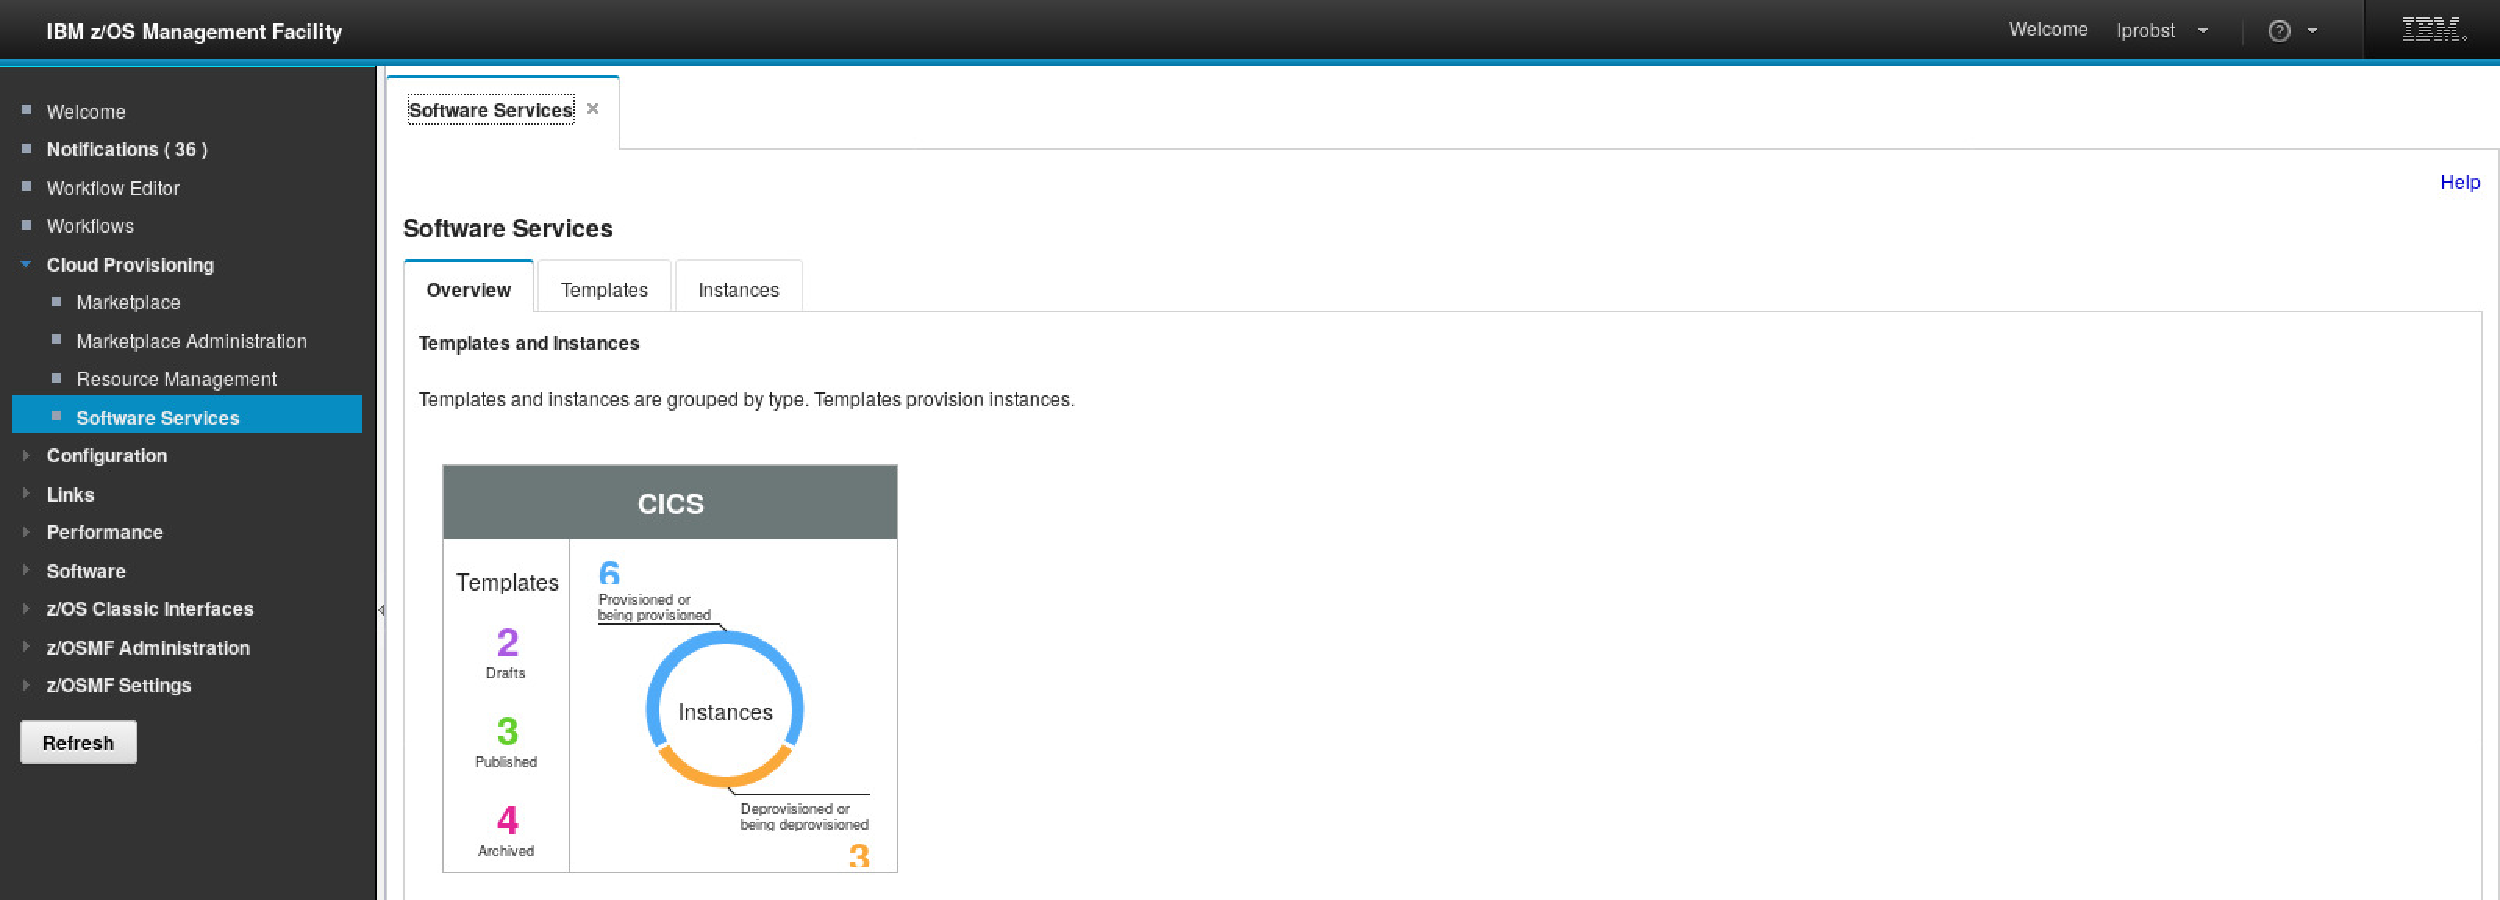
\includegraphics[scale=0.32]{images/kapitel_3/zosmf_softwareservice.pdf}
  \caption{Übersicht der CICS-Regionen}
  \label{fig:zosmfsoftwareservice}
\end{figure}

Über den Reiter \path{Templates} kann die Übersicht über alle angelegten Templates angezeigt werden. Über den Button
\path{Create} kann ein neues Software Service Template eingerichtet werden. Als Name wird hier
\path{cics53_mas_liberty_ucd} angegeben.

Dieser Workflow muss einerseits die CICS-Region in der CICS-Runtime hinzufügen und anmelden. Außerdem muss aus einem
vorgegebenen Pool an Port-Nummern eine ausgewählt und der CICS-Region konfiguriert werden.

Sobald die CICS-Region erfolgreich eingerichtet wurde, muss diese an dem UCD angemeldet werden, damit im späteren
Verlauf auch Anwendungen über UCD auf der Region installiert und eingerichtet werden können.

Nach der Speicherung des Templates wird dies in der Liste aller Templates angezeigt. Ein Klick auf dieses öffnet die
detaillierten Informationen darüber. Siehe dazu Abbildung \ref{fig:zosmftemplate} auf Seite \pageref{fig:zosmftemplate}.

\begin{figure}[h]
  \centering
    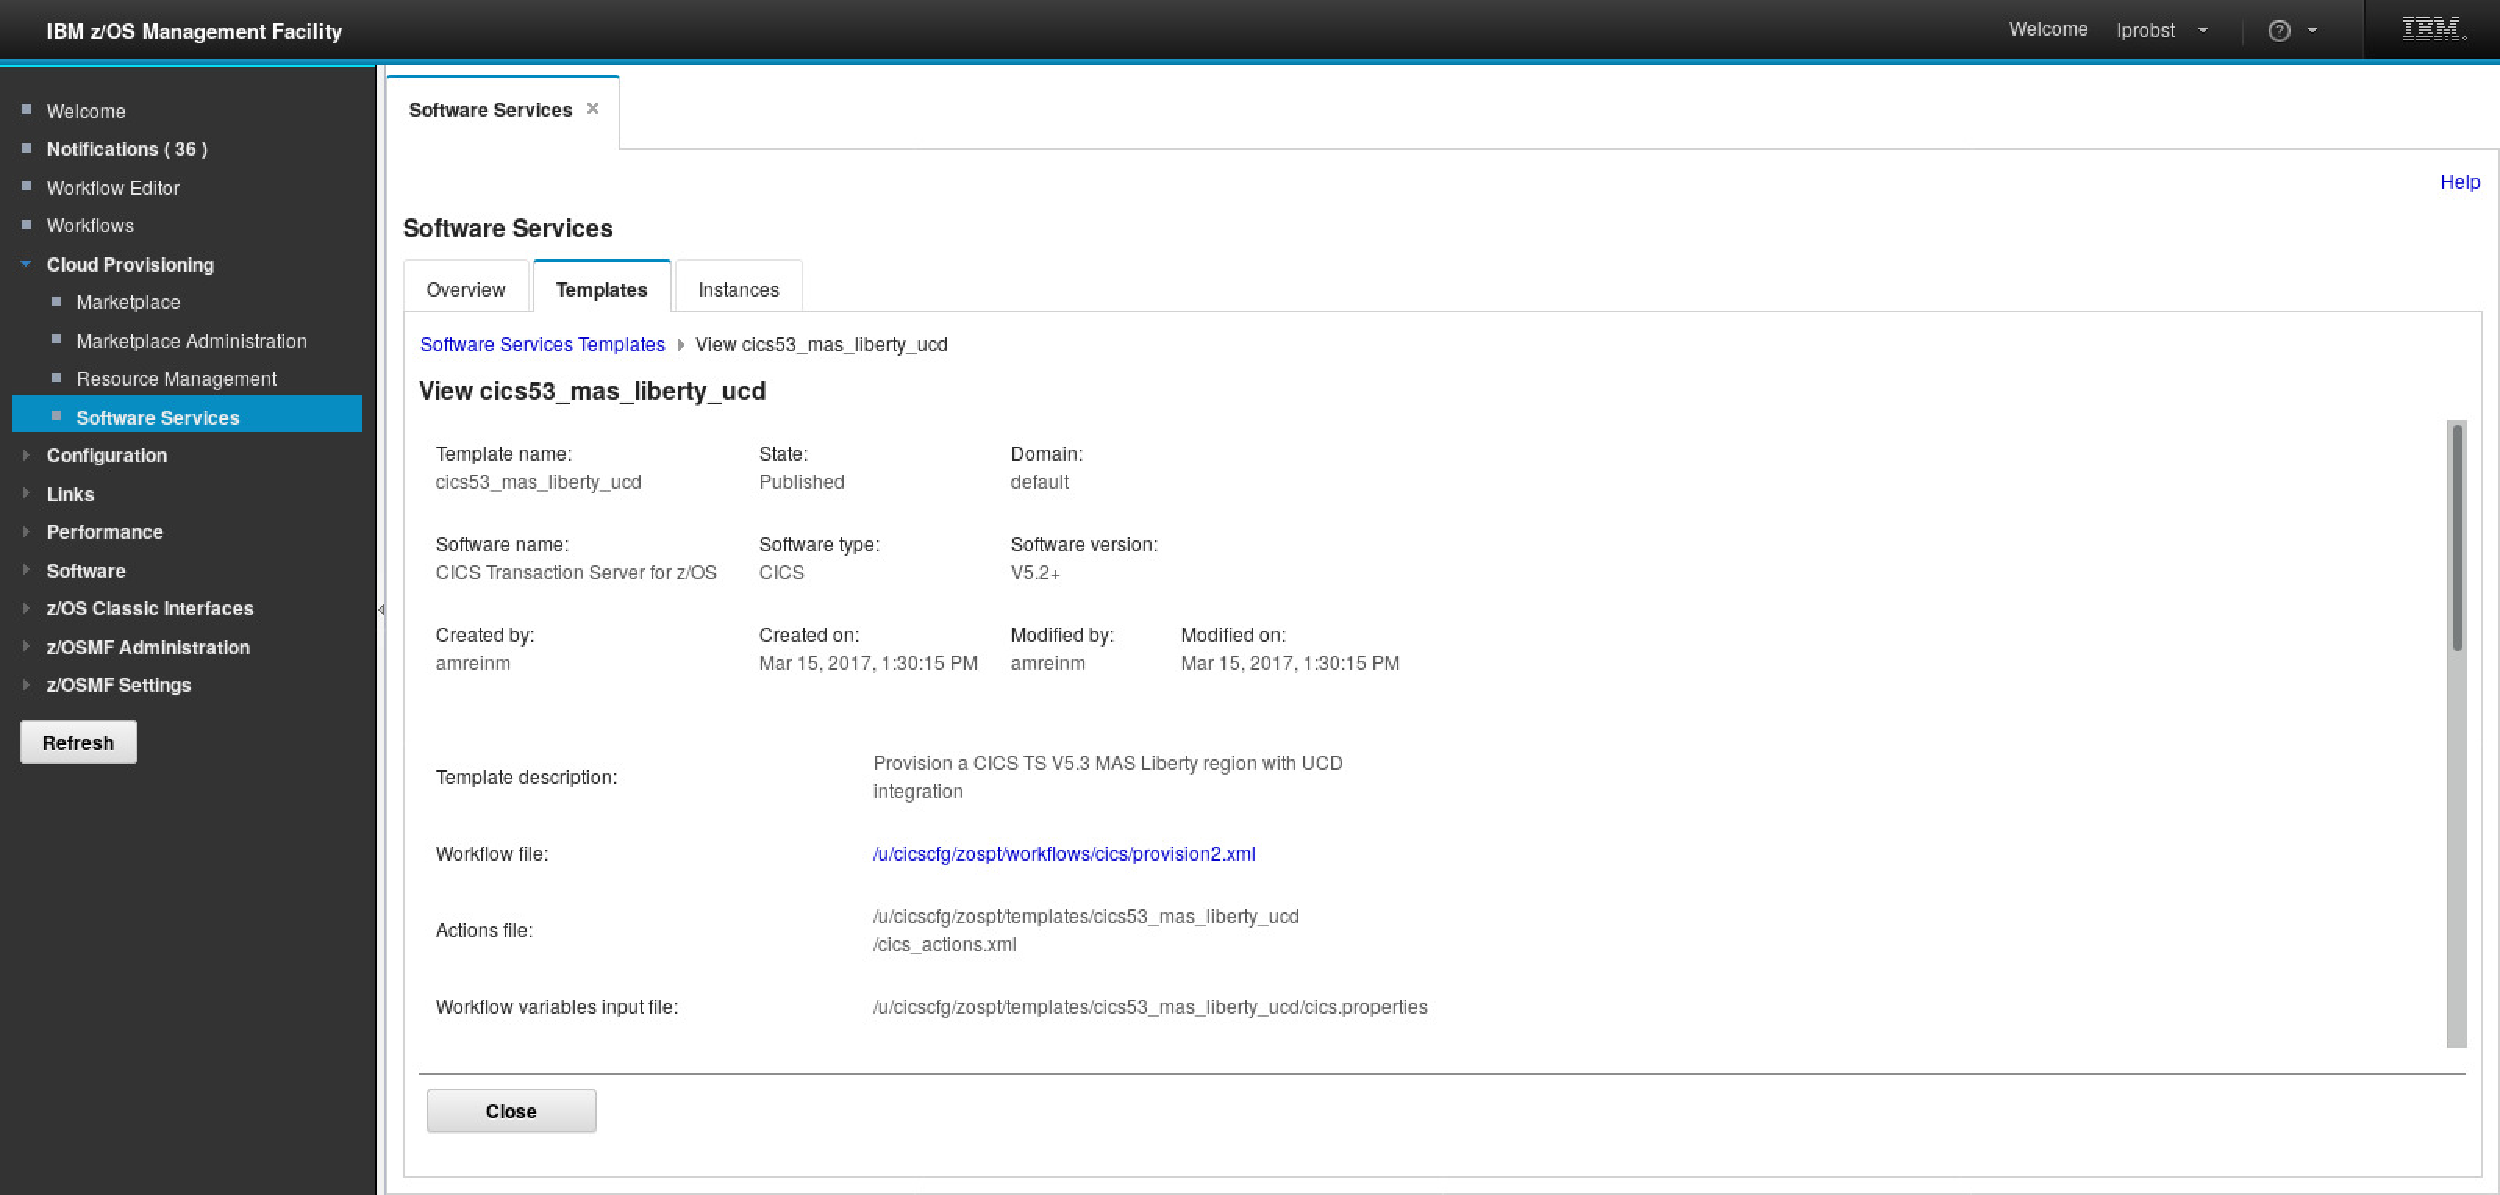
\includegraphics[scale=0.32]{images/kapitel_3/zosmf_template.pdf}
  \caption{Informationen des eingerichteten Software Service Templates}
  \label{fig:zosmftemplate}
\end{figure}

\subsection{RACF Profil einrichten}
Unter z/OS werden neben Identifikation und Verifikation von Benutzern und deren Protokollierung auch die Zugriffe
auf Resourcen über RACF Profile verwaltet. Diese implementieren die System Authorization Facility (kurz SAF) des Kernels
(MVS).

Um einem Benutzer oder einem Programm Zugriff auf Resourcen zu gewähren, müssen dafür RACF-Profile eingerichtet werden.

Für die Nutzung der zOSMF RESTFul-"-Schnittstelle müssen die in Listing \ref{RACF Profil einrichten} auf Seite
\pageref{RACF Profil einrichten} aufgeführten Kommandos ausgeführt werden.

Die Befehle werden als Administrator des Systems in die Kommandozeile (Terminal) eingegeben. Erst dann funktioniert die
RESTFul-Schnittstelle des zOSMF.

\begin{lstlisting}[language=bash, caption=RACF Profil einrichten, label=RACF Profil einrichten]
   $ RDEFINE ZMFAPLA IZUDFLT.REST.** UACC(NONE)
   $ PERMIT IZUDFLT.REST.** CLASS(ZMFAPLA) ID(IZUSVR) ACCESS(READ)
   $ SETROPTS RACLIST(ZMFAPLA) REFRESH
\end{lstlisting}

Ob die Einrichtung funktioniert hat, kann durch den Aufruf der RESTFul-Schnittstelle überprüft werden. Dazu werden z.B.
die Information der zOSMF Instanz durch die Schnittstelle abgerufen. Die URL ist die im Secure Gateway definierte mit der
Endung \path{/zosmf/info}. Die URL sollte wie folgt aussehen: \path{https://securegatewayUrl:securegatewayPort/zosmf/info}.

Alternativ kann im gleichen Netzwerk auch die IP-Adresse des Systems verwendet werden. Dann muss allerdings der Port
\path{60443} genutzt werden, da dies der Standardport für die Schnittstelle ist. In diesem Fall setzt sich die URL wie
folgt zusammen: \path{https://ipMainframe:60443/zosmf/info}.

\subsection{Einrichten des Secure Gateways}
\label{subsection:secureGateway}
Für die Kommunikation zwischen Bluemix (Cloud) und z System (Lokal) wird eine dauerhafte Verbindung benötigt. Die Umsetzung
erfolgt durch den Secure Gateway-Service von Bluemix. Dieser befindet sich im Bluemix-Katalog im Bereich \path{Integrate}.

Nach der Instanziierung des Services kann dieser angeklickt werden, wodurch sich die Konfigurationsansicht öffnet. Dort
befindet sich im Bereich \path{Verwalten} die Möglichkeit, ein neues Gateway hinzuzufügen. Dazu wird, nach einem Klick auf
das weiße \textit{Plus}, lediglich ein Name eingegeben. Ein Beispiel hierfür ist \path{Mainframe}.

Nun wird über den Tab \path{Clients} dem Gatway ein neuer Client hinzugefügt. In dem sich öffnenden Fenster wird die
Gateway-ID und der Sicherheitstoken für den neuen Client angezeigt. Diese müssen notiert werden, da sie nicht noch einmal
angezeigt werden können.

Anschließend wird der passende Client für die Systemarchitektur heruntergeladen und auf dem Zielsystem installiert.

\begin{lstlisting}[language=bash, caption=Secure Gateway für s390x installieren, label=Secure Gateway s390x installieren]
   $ wget https://sgmanager.ng.bluemix.net/installers/ibm-securegateway-client-1.7.1+client_s390x.deb
   $ sudo dpkg -i ibm-securegateway-client-1.7.1+client_s390x.deb
\end{lstlisting}

Während der Installation wird nach der notierten Gateway-ID und dem Sicherheitstoken gefragt. Nach erfolgreicher Installation
erscheint der neue Client in Bluemix im Reiter \path{Clients}.

Standardmäßig lässt der Secure Gateway nur Verbindungen zu, welche in einer ACL-Datei (Access Control List) aufgeführt sind.
Damit die Ubuntu-Maschine nun mit jeweils dem RedHat- und dem z/OS-System kommunizieren kann, wird im Ordner
\path{/opt/ibm/SecureGateway/client} eine Datei namens \path{ACL.txt} angelegt.

\begin{lstlisting}[language=bash, caption=ACL-Datei anlegen, label=ACL-Datei anlegen]
   $ cd /opt/ibm/SecureGateway/client
   $ touch ACL.txt
\end{lstlisting}

In der \path{ACL.txt}-Datei müssen nun die folgenden Zeilen eingefügt werden. Links vom Doppelpunkt werden die jeweiligen
lokalen IP-Adressen eingetragen, und nach dem Doppelpunkt können die Ports angegeben werden. Die Ports werden hier allerdings
nicht benötigt und deshalb leer gelassen. Die Verbindung zu den einzelnen Systemen soll hier nicht eingeschränkt werden.

\begin{lstlisting}[language=bash, caption=Inhalt der ACL-Datei, label=Inhalt der ACL-Datei]
   acl allow 10.3.20.47:
   acl allow 10.3.20.233:
\end{lstlisting}

Nun muss in der Konfigurationsdatei des installierten Clients die ACL.txt-Datei angegeben werden. Dazu wird im Ordner
\path{/etc/ibm/} die Datei \path{sgenvironment.conf} bearbeitet. In Zeile 18 muss der folgende Inhalt eingefügt werden:

\begin{lstlisting}[language=bash, numbers=left, firstnumber=18, caption=Konfigurationsdatei anpassen, label=Konfigurationsdatei anpassen]
   ACL_FILE=/opt/ibm/securegateway/client/ACL.txt
\end{lstlisting}

Damit können nun unter allen Ports Verbindungen zu den beiden Maschinen \path{10.3.20.47} und \path{10.3.20.233} aufgebaut
werden. Das ist wichtig, damit in Bluemix mehrere Routen (Ziele) definiert werden können.

Im Anschluss können nun Ziele für den installierten Gateway hinzugefügt werden. Ziele sind dabei immer Rechner, Programme
oder Schnittstellen im Netzwerk des Gateways, die in der \path{ACL.txt}-Datei angegeben wurden oder er selbst. Außerdem
können die Ports für die Verbindung angegeben werden.

Als erstes Ziel wird eine Verbindung zum zOSMF eingerichtet. Der Name hierfür ist \path{zOSMF}. Die IP-Adresse ist das
z/OS System mit \path{10.3.20.47} und der Port ist der der RESTFul-Schnittstelle von zOSMF mit \path{60443}. Als Protokoll
wird \path{https} ausgewählt.

Das zweite Ziel wird die Verbindung zu UCD repräsentieren. Dazu wird ein neues Ziel hinzugefügt und als Name \path{UCD}
und als IP-Adresse die des RedHat-Systems, \path{10.3.20.233}, eingetragen. Der Port der RESTFul-Schnittstelle von UCD
ist \path{8443}, und als Protokoll wird ebenfalls \path{https} ausgewählt.

Als letztes wird noch ein drittes Ziel - für den DB2 Service - hinzugefügt. Der Name ist dabei \path{DB Service}, die
IP-Adresse die des z/OS-Systems, welches die DB Instanz hält mit \path{10.3.20.47} und als Port der DB2 Service Port mit
\path{4740}.

Nun erstellt der Secure Gateway-Service in Bluemix drei individuelle Domains mit zugehörigen  Ports für die jeweiligen
Verbindungen. In diesem Fall ist dies \path{https://cap-sg-prd-1.integration.ibmcloud.com:16283} für das zOSMF-Interface,
\path{https://cap-sg-prd-1.integration.ibmcloud.com:15543} für die UCD Verbindung und als letzte Domain
\path{http://cap-sg-prd-1.integration.ibmcloud.com:16950} für den DB2 Service.

Da die URL mit dem Port auf die lokale IP des Mainframes mit dem zOSMF-Port gemappt wird, kann im Browser das zOSMF mit
der URL aufgerufen werden, ohne dass man sich im Netzwerk des Mainframes befinden muss. Das selbe gilt auch für UCD und
den DB2 Service.

Nun besteht eine Verbindung zwischen Bluemix und dem lokalem Mainframe, die ab sofort genutzt und beliebig erweitert
werden kann.

\subsection{Schreiben eines Service Brokers}
\label{subsection:writeservicebroker}
Da das zOSMF nun auch von außerhalb des lokalen Netzwerkes aufrufbar ist, kann nun der Service Broker entwickelt werden,
der die Ressourcen in Form von CICS-Regionen auf dem Mainframe bereitstellen soll. Dazu greift der Service Broker über den
Secure Gateway auf die RESTFul-Schnittstellen von zOSMF bzw. UCD zu.

Um einen Service Broker in Bluemix anbieten zu können, muss dieser in einem Container laufen und via URL aufrufbar sein.
In diesem Container läuft die Service Broker Anwendung, welche neben einem REST-Interface auch das Konfigurationsinterface
zur Verfügung stellt.

Das REST-Interface wird von einem Bluemix-Nutzer einmalig genutzt, um eine Service-Instanz zu erstellen, diese zu
konfigurieren oder zu löschen. Bei der Erstellung kann der Nutzer angeben, welchen \path{Plan} er nutzen möchte.

Mit dem Konfigurationsinterface kann jeder Benutzer individuell seinen instanziierten Service konfigurieren und erweitern.

Eine Übersicht über die Architektur eines Service Brokers ist in Abbildung \ref{fig:architektur_servicebroker} auf Seite
\pageref{fig:architektur_servicebroker} zu finden.

\begin{figure}[h]
  \centering
    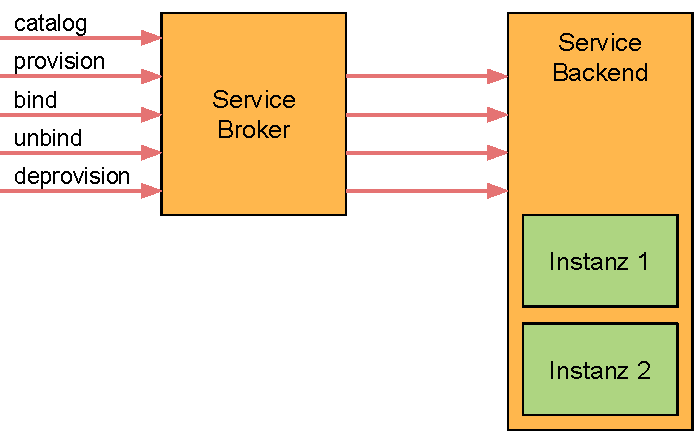
\includegraphics[scale=0.9]{images/kapitel_3/architektur_servicebroker.pdf}
  \caption{Allgemeine Architektur eines Service Brokers}
  \label{fig:architektur_servicebroker}
\end{figure}

In dieser Abbildung ist zu sehen, dass der Service Broker die Funktionen \path{catalog}, \path{provision}, \path{bind},
\path{unbind} und \path{deprovision} umsetzen muss.

Bei \path{catalog} wird der Katalog des Service Brokers zurückgegeben und der Nutzer kann sich diese anschauen.

Die Funktion \path{provision} ermöglicht die Instantiierung des Service Brokers in einer Bluemix Umgebung.

Bei \path{bind} handelt es sich um das Verbinden eines Services und einer Runtime um Daten über die VCAP-Variablen
auszutauschen.

\path{Unbind} löst eine schon geschaffene Verbindung wieder auf und \path{deprovision} löscht den instanziierten Service
Broker komplett aus dem eigenen Bluemix Bereich.

In dieser Arbeit wird der Service Broker in der Programmiersprache \path{Python}\footnote{https://www.python.org}
geschrieben. Dazu wird in Bluemix ein Python Cloud Foundry-Container aus der Katalog Kategorie
\path{Cloud Foundry-Anwendungen} erstellt.

Anschließend wird in der Übersicht, in der gerade erstellten Anwendung, im Bereich \path{Continuous Delivery} ein JazzHub
Git-Repository hinzugefügt. In diesem wird der Quellcode abgelegt und nach einem \path{push} durch Git ein automatischer
Buildprozess angestoßen, welcher den Service Broker bereitstellt.

Um mit der Entwicklung zu beginnen, wird zuallererst das Git-Repository auf den eigenen Rechner geklont. Dazu wird mit
Hilfe des \path{clone}-Befehls von Git dieses kopiert.

\begin{lstlisting}[language=bash, caption=Git-Repository Klonen, label=Git-Repository Klonen]
   $ git clone https://hub.jazz.net/benutzerName/anwendungsName
\end{lstlisting}

Dabei ist der Pfad \path{benutzerName} der Benutzername des Accounts, welcher den Cloud Foundry Container erstellt hat
und \path{anwendungsName} der Name des Containers. Die vollständige URL kann jedoch auch nach dem Ertellen des Repositorys
kopiert werden.

Wenn der Klonvorgang erfolgreich ist, wird auf dem Entwicklungsrechner ein Ordner mit dem Namen der Cloud Foundry
Anwendung erstellt, in welchem Beispieldaten für eine Python-Anwendung für Bluemix hinterlegt sind.

Nach der Analyse des Service Brokers und der Schnittstellen die dieser zur Verfügung stellen muss, kann dieser entwickelt
werden. Eine Dokumentation der zu implementierenden Schnittstellen ist in  Abbildung \ref{fig:swagger_servicebroker} auf
Seite \pageref{fig:swagger_servicebroker} zu sehen.

\begin{figure}[h]
  \centering
    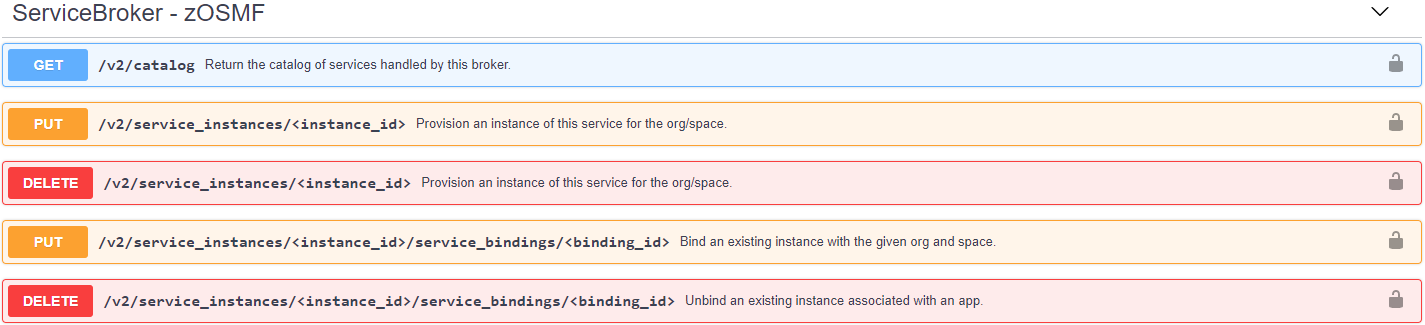
\includegraphics[scale=0.38]{images/kapitel_3/swagger_servicebroker.png}
  \caption{Schnittstellen des Service Brokers}
  \label{fig:swagger_servicebroker}
\end{figure}

Damit die Anwendung in Python geschrieben werden kann, werden drei Libraries benötigt. Diese werden in eine Datei mit
Namen \path{requirements.txt} gespeichert. Bei den Abhängigkeiten handelt es sich um \path{Flask}, \path{flask_basicauth}
und \path{uuid}.

\path{Flask} wird benötigt, um realtiv einfach ein REST-Interface in Pyhton bereit stellen zu können, welches über
mehrere Endpunkte verfügt.

Bei \path{flask_basicauth} handelt es sich um ein Plugin für Flask, welches es ermöglicht einzelne Routen über eine
Authentifizierung zu sichern. Das wird benötogt, da das erstellen einer Instanz des Service Brokers laut Definition eine
Authentifizierung vorsieht.

Mit \path{uuid} können einmalige Identifikatoren erstellt werden, welche jede Instanz des Service Brokers eindeutig
identifizieren können. Auch diese Eigenschaft wird laut Definition eines Service Brokers benötigt.

Wenn die Cloud Foundry-Runtime nach einem Upload der Daten gebaut wird, werden automatisch alle Abhängigkeiten, welche
in der \path{requirements}-Datei angegeben sind, heruntergeladen und bereitgestellt.

Anschließend wird in der \path{runtime.txt}-Datei angegeben, in welcher Python-Version die Anwendung laufen soll. In diesem
Beispiel wird \path{python-3.5.1} genutzt.

Auch hier kümmert sich die Cloud Foundry-Runtime automatisch um die Bereitstellung der geforderten Version der Runtime.

Damit Pyhton wissen kann um welche art der Anwendung es sich handelt, wird in der \path{Procfile}-Datei angegeben, wie
die Anwendung gestartet werden und welche Datei beim Start ausgeführt werden soll. Der Inhalt der Datei ist
\path{web: python app/main.py}. Dadurch wird definiert, dass es sich um eine \textit{web}-Anwendung handelt und die Datei
\textit{main.py} im Verzeichnis \textit{app} ausgeführt werden soll. Dies ist auch die einzige Python-Datei in dem
Projekt.

Im Verzeichnis \path{/app} gibt es nun mehrere Unterverzeichnisse und eine Datei.

Im \path{/app/templates}-Ordner wird das Template hinterlegt, welches der Nutzer sieht wenn er den Service instanziiert
hat und ihn nun konfigurieren möchte, das Dashboard.

Im \path{/app/static} Verzeichnis sind Ordner und Dateien die für die Darstellung des Dashbaords wichtig sind. Dort wird
das eigentliche Design und der Aufbau des Dashboards erstellt.

In der \path{app/main.py}-Datei werden unter anderem der Benutzername und das Passwort zum Erstellen einer Instanz definiert
und die Pläne die es für den Service geben soll.

Außerdem werden in der unteren Hälfte die REST-Endpunkte zum instanziiere, editieren, binden und löschen eines Service
Brokers für den Nutzer definiert. Diese sind von Cloud Foundry vorgegeben und müssen lediglich implementiert werden.
Bluemix kümmert sich beim instanziieren des Service Brokers um den richtigen Aufruf des Interfaces.

Nach der Entwicklung des Service Brokers können die Änderungen am Quellcode mit dem Git-Befehl \path{commit} gespeichert
werden. Hinter dem Parameter \path{m} kann eine Nachricht angegeben werden, welche die Änderung beschreibt.

\begin{lstlisting}[language=bash, caption=Änderungen speichern, label=Änderungen speichern]
   $ git commit -m "Update all files"
\end{lstlisting}

Anschließend können mit \path{push} alle gespeicherten Änderungen an das Git-Repository übertragen werden.

\begin{lstlisting}[language=bash, caption=Änderungen hochladen, label=Änderungen hochladen]
   $ git push
\end{lstlisting}

Der Continous Deployment Service, welcher automatisch mit dem Hinzufügen eines Git-Repositorys zu einer Anwendung
hinzugefügt wird, registirert den \path{push} in das Repository und baut ein neues Artefakt, welches in den Cloud Foundry
Container geladen und bereitgestellt wird.

Das Dashboard des entwickelten Service Brokers ist in Abbildung \ref{fig:servicebroker_oberflaeche} auf Seite
\pageref{fig:servicebroker_oberflaeche} zu sehen und der komplette Quellcode ist im öffentlichen
GitHub-\-Repository\footnote{https://github.com/Alienuser/ServiceBroker-zOSMF} hinterlegt.

\begin{figure}[h]
  \centering
    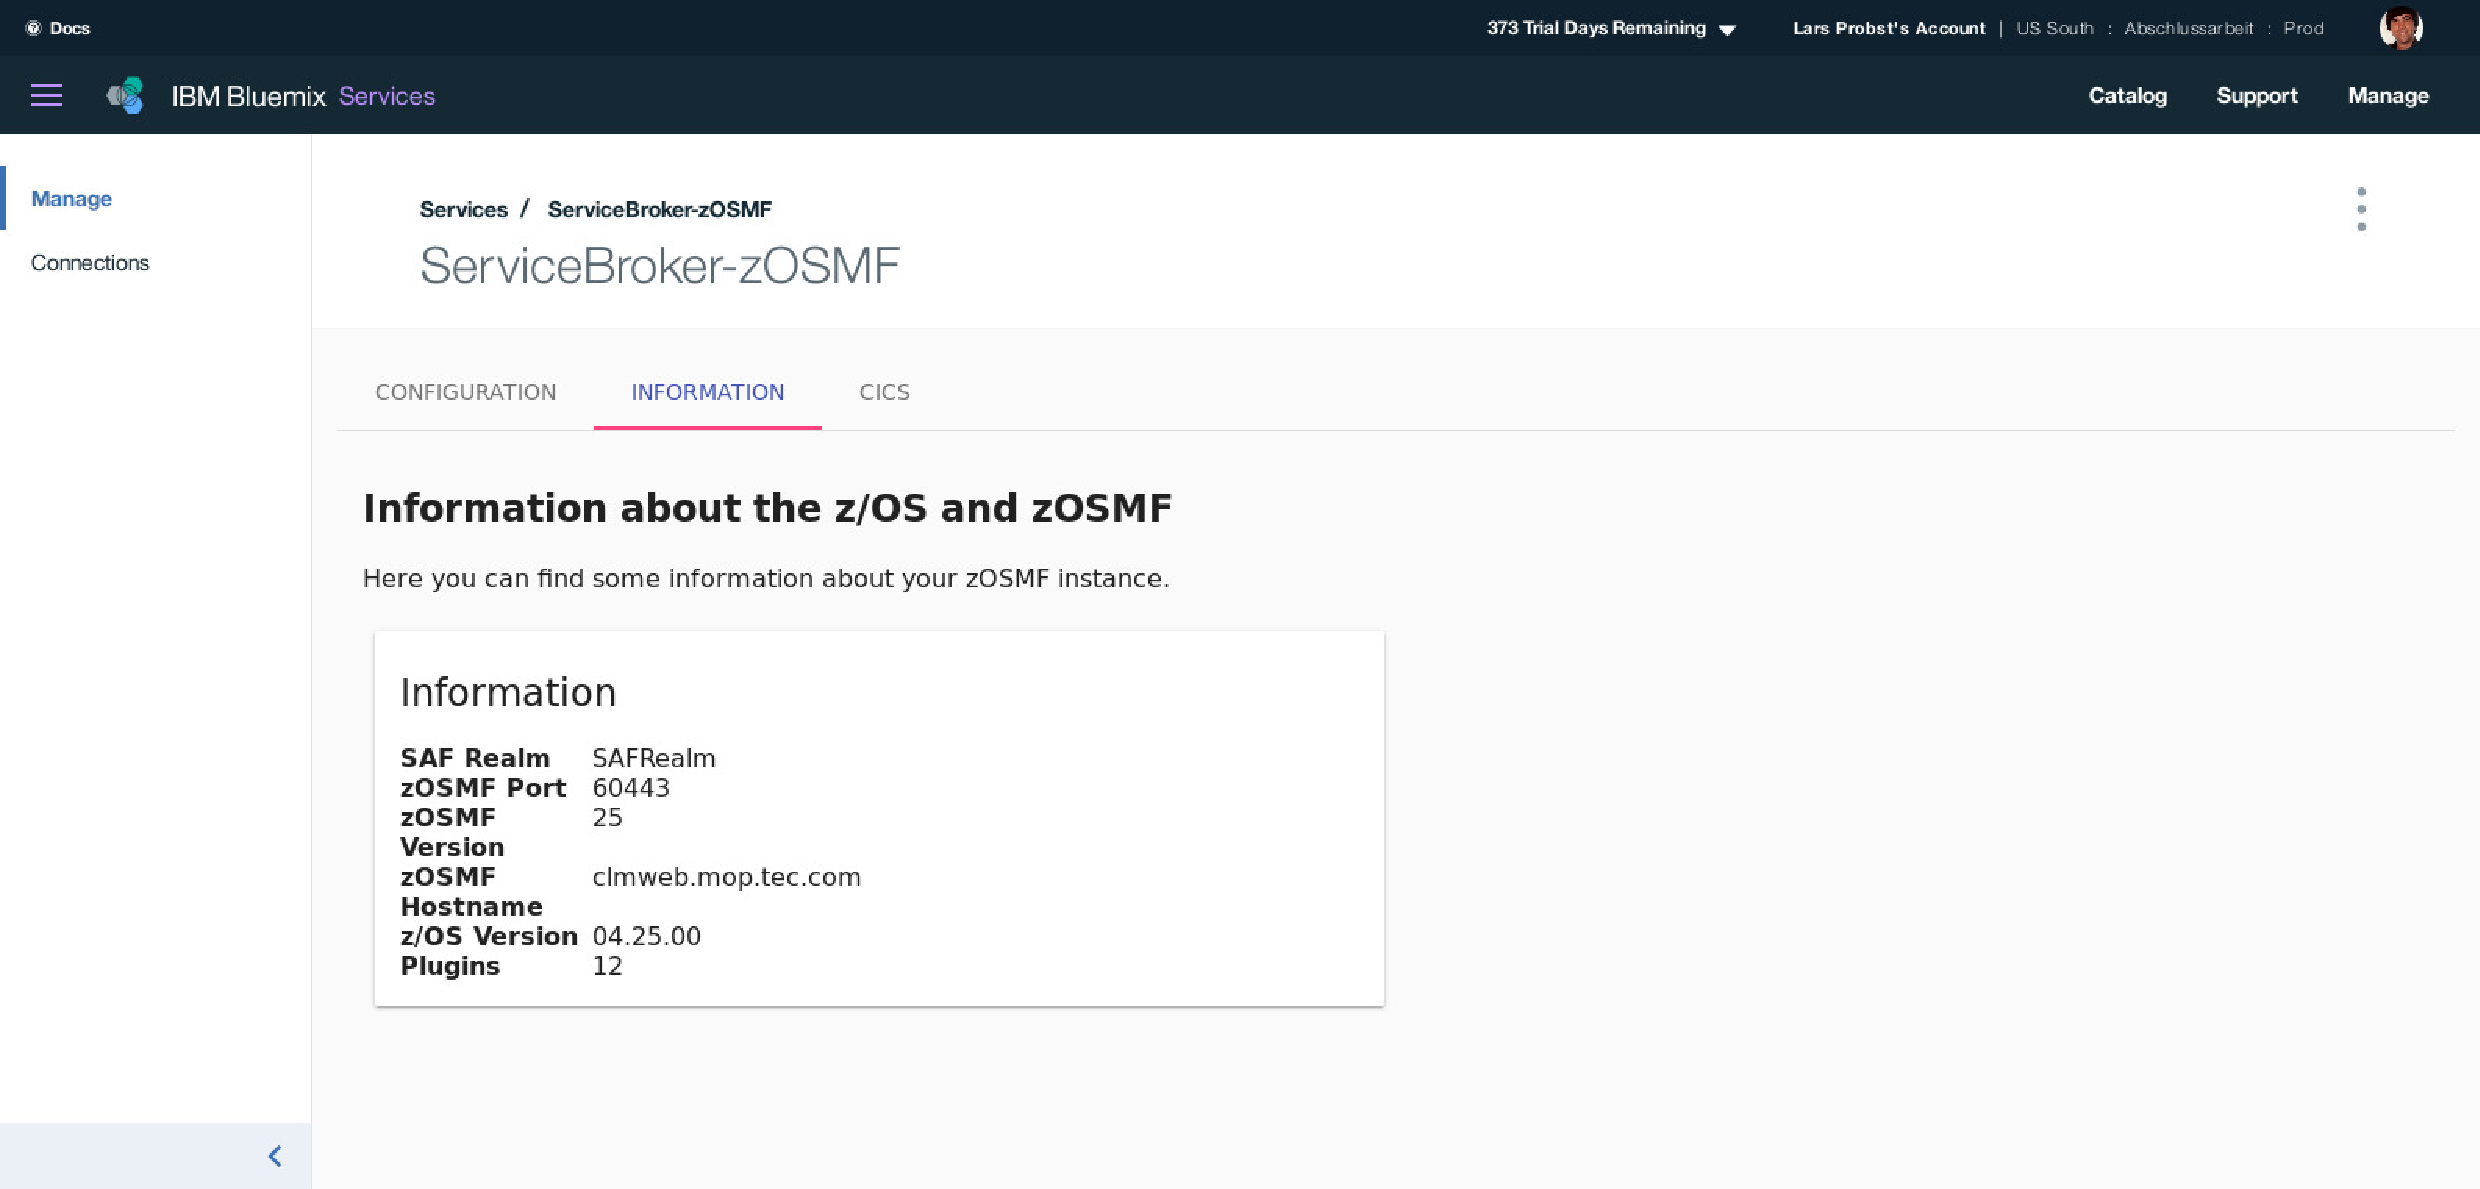
\includegraphics[scale=0.31]{images/kapitel_3/servicebroker_oberflaeche.pdf}
  \caption{Web-Interface des Service Brokers}
  \label{fig:servicebroker_oberflaeche}
\end{figure}

Nun läuft der Service Broker in einem Cloud Foundry Container und verfügt über eine eindeutige URL, über die er aufgerufen
werden kann. Dies ist für die weiteren Schritte wichtig.

Eine Übersicht über alle wichtigen Funktionen der RESTFul-Schnittstelle von zOSMF ist auf der
Hilfeseite\footnote{https://www.ibm.com/support/knowledgecenter/SSLTBW\_2.2.0/RESTServices.htm} zu finden.

\subsection{Instanziieren des Service Brokers}
Der geschriebene Service Broker, welcher nun unter Bluemix als Cloud Foundry-Applikation läuft, kann nun als Service
instanziiert werden.

Da die Anwendung in Bluemix Public läuft, kann der Service Broker nur als \path{Space Scoped} Broker hinzugefügt
werden, vergleiche dazu Kapitel \ref{sub:scopes} auf Seite \pageref{sub:scopes}.

Um den Service Broker in die eigene Organisation hinzuzufügen, muss zuallererst die Cloud Foundry CLI mit dem eigenen
Bluemix-Account und der Zielorganisation verbunden werden. Dazu wird im Terminal der \path{api}-Befehl ausgeführt.

\begin{lstlisting}[language=bash, caption=Definieren der API über die Cloud Foundry CLI, label=Definieren der API über die Cloud Foundry CLI]
   $ cf api api.ng.bluemix.net
\end{lstlisting}

Nun ist die Cloud Foundry CLI mit der amerikanischen Instanz von Bluemix verbunden, in die man sich nun mittels
\path{login} einloggen kann.

\begin{lstlisting}[language=bash, caption=Einloggen über die Cloud Foundry CLI, label=Einloggen über die Cloud Foundry CLI]
   $ cf login
\end{lstlisting}

Im Folgenden wird nach der E-Mail-Adresse und dem dazugehörigen Passwort des Bluemix-Accounts gefragt. Nach korrekter
Eingabe der Daten wird nach der Organisation gefragt, mit welcher das CLI verbunden werden soll.

Nach Eingabe der entsprechenden Zahl ist die Cloud Foundry CLI erfolgreich mit der Zielorganisation verbunden, und der
Service Broker kann dieser hinzugefügt werden.

Sollten in der Organisation mehrere Bereiche vorhanden sein, wird im Anschluss noch nach einer entsprechenden Auswahl
gefragt. Dabei ist egal, welcher Bereich ausgewählt wird, da der Service Broker in der kompletten Organisation zur Verfügung
steht.

Nun kann der Service Broker in die Organisation hinzugefügt werden. Dies geschieht über den Befehl \path{create-service-broker}.

\begin{lstlisting}[language=bash, caption=Service Broker einrichten, label=Service Broker einrichten]
   $ cf create-service-broker brokerName username password brokerURL --space-scoped
\end{lstlisting}

Dabei ist \path{brokerName} der Name des in Kapitel \ref{subsection:writeservicebroker} auf Seite
\pageref{subsection:writeservicebroker} angelegten Service Brokers.

Die Parameter \path{username} und \path{password} sind nicht die des Bluemix-Benutzerkontos, sondern die für den Zugriff
auf den Service Broker.

Die \path{brokerURL} ist die URL der Cloud Foundry-Applikation, in der der Service Broker aufrufbar ist.

Der letzte Parameter \path{--space-scoped} ist wichtig, da damit der Scope des Service Brokers angegeben wird. Wird dieser
bei der Nutzung von Bluemix Public weggelassen, erscheint eine Fehlermeldung.

Nach der Eingabe des Befehls sollte eine Information erscheinen, welche das erfolgreiche Hinzufügen des Service Brokers
quittiert.

Über die Cloud Foundry CLI gibt es zwei Möglichkeiten die aktuellen Services einzusehen, die für den Benutzer in der
Organisation zur Verfügung stehen. Der Befehl \path{marketplace} listet \textbf{alle} verfügbaren Services auf.

\begin{lstlisting}[language=bash, caption=Auflisten aller verfügbaren Services, label=Auflisten aller verfügbaren Services]
   $ cf marketplace
\end{lstlisting}

Wohingegen der \path{service-brokers}-Befehl nur die selbst (oder von einem eingeladenen Account) hinzugefügten Service
Broker auflistet.

\begin{lstlisting}[language=bash, caption=Auflisten aller Service Broker, label=Auflisten aller Service Broker]
   $ cf service-brokers
\end{lstlisting}

\subsection{Provisionieren des Service Brokers}
Da der Service Broker nun als solcher in der Bluemix Organisation eingerichtet wurde, kann eine Instanz des Services
für einen Bereich (Space) provisioniert werden.

Jeder Service kann nur in einem Bluemix-Bereich provisioniert werden. Für die kommenden Schritte ist es wichtig,
dass der richtige Bereich in der Cloud Foundry CLI ausgewählt ist. Über den \path{target}-Befehl kann der Bereich
neu definiert werden.

\begin{lstlisting}[language=bash, caption=Bereich (Space) in Cloud Foundry CLI wechseln, label=Bereich (Space) in Cloud Foundry CLI wechseln]
   $ cf target -s spaceName
\end{lstlisting}

Der Parameter \path{spaceName} gibt den Bereich an, der ausgewählt werden soll.

Die Provisionierung eines Services geschieht über den \path{create-service}-Befehl der Cloud Foundry CLI.

\begin{lstlisting}[language=bash, caption=Provisionieren eines Services, label=Provisionieren eines Services]
   $ cf create-service service servicePlan serviceName
\end{lstlisting}

Der Parameter \path{service} gibt den Service Broker an, welcher provisioniert werden soll. Das ist der \path{brokerName}-
Parameter aus Listing \ref{Service Broker einrichten} auf Seite \pageref{Service Broker einrichten}.

Der \path{servicePlan} gibt den Plan an, welcher genutzt werden soll. Zur Auswahl stehen die im Service Broker
konfigurierten.

Als letztes wird über \path{serviceName} ein Name vergeben, wie der Service in Bluemix genannt werden soll. Über diesen
wird er im Bluemix Dashboard angezeigt. Über den Namen kann er später auch verändert oder gelöscht werden. In diesem Beispiel
wird der Service Borker \path{Service Broker zOSMF} genannt.

Nun kann der provisionierte Service mit dem vergebenen Namen im Bluemix Dashbaord in der entsprechenden Organisation und
dem Bereich eingesehen werden. Ein Klick auf den Service öffnet die Informationsseite des Services.

\subsection{Nutzen des Service Brokers}
Da der Service Broker nun instanziiert ist, kann er in Bluemix genutzt werden. Folgend wird der Service Broker kurz
eingerichtet und die wichtigsten Optionen erklärt.

Dazu wird dieser aus dem Bluemix Dashboard geöffnet. Es erscheint die Ansicht der Konfiguration wie in Abbildung
\ref{fig:servicebroker_configuration} auf Seite \pageref{fig:servicebroker_configuration} zu sehen.

\begin{figure}[h]
  \centering
    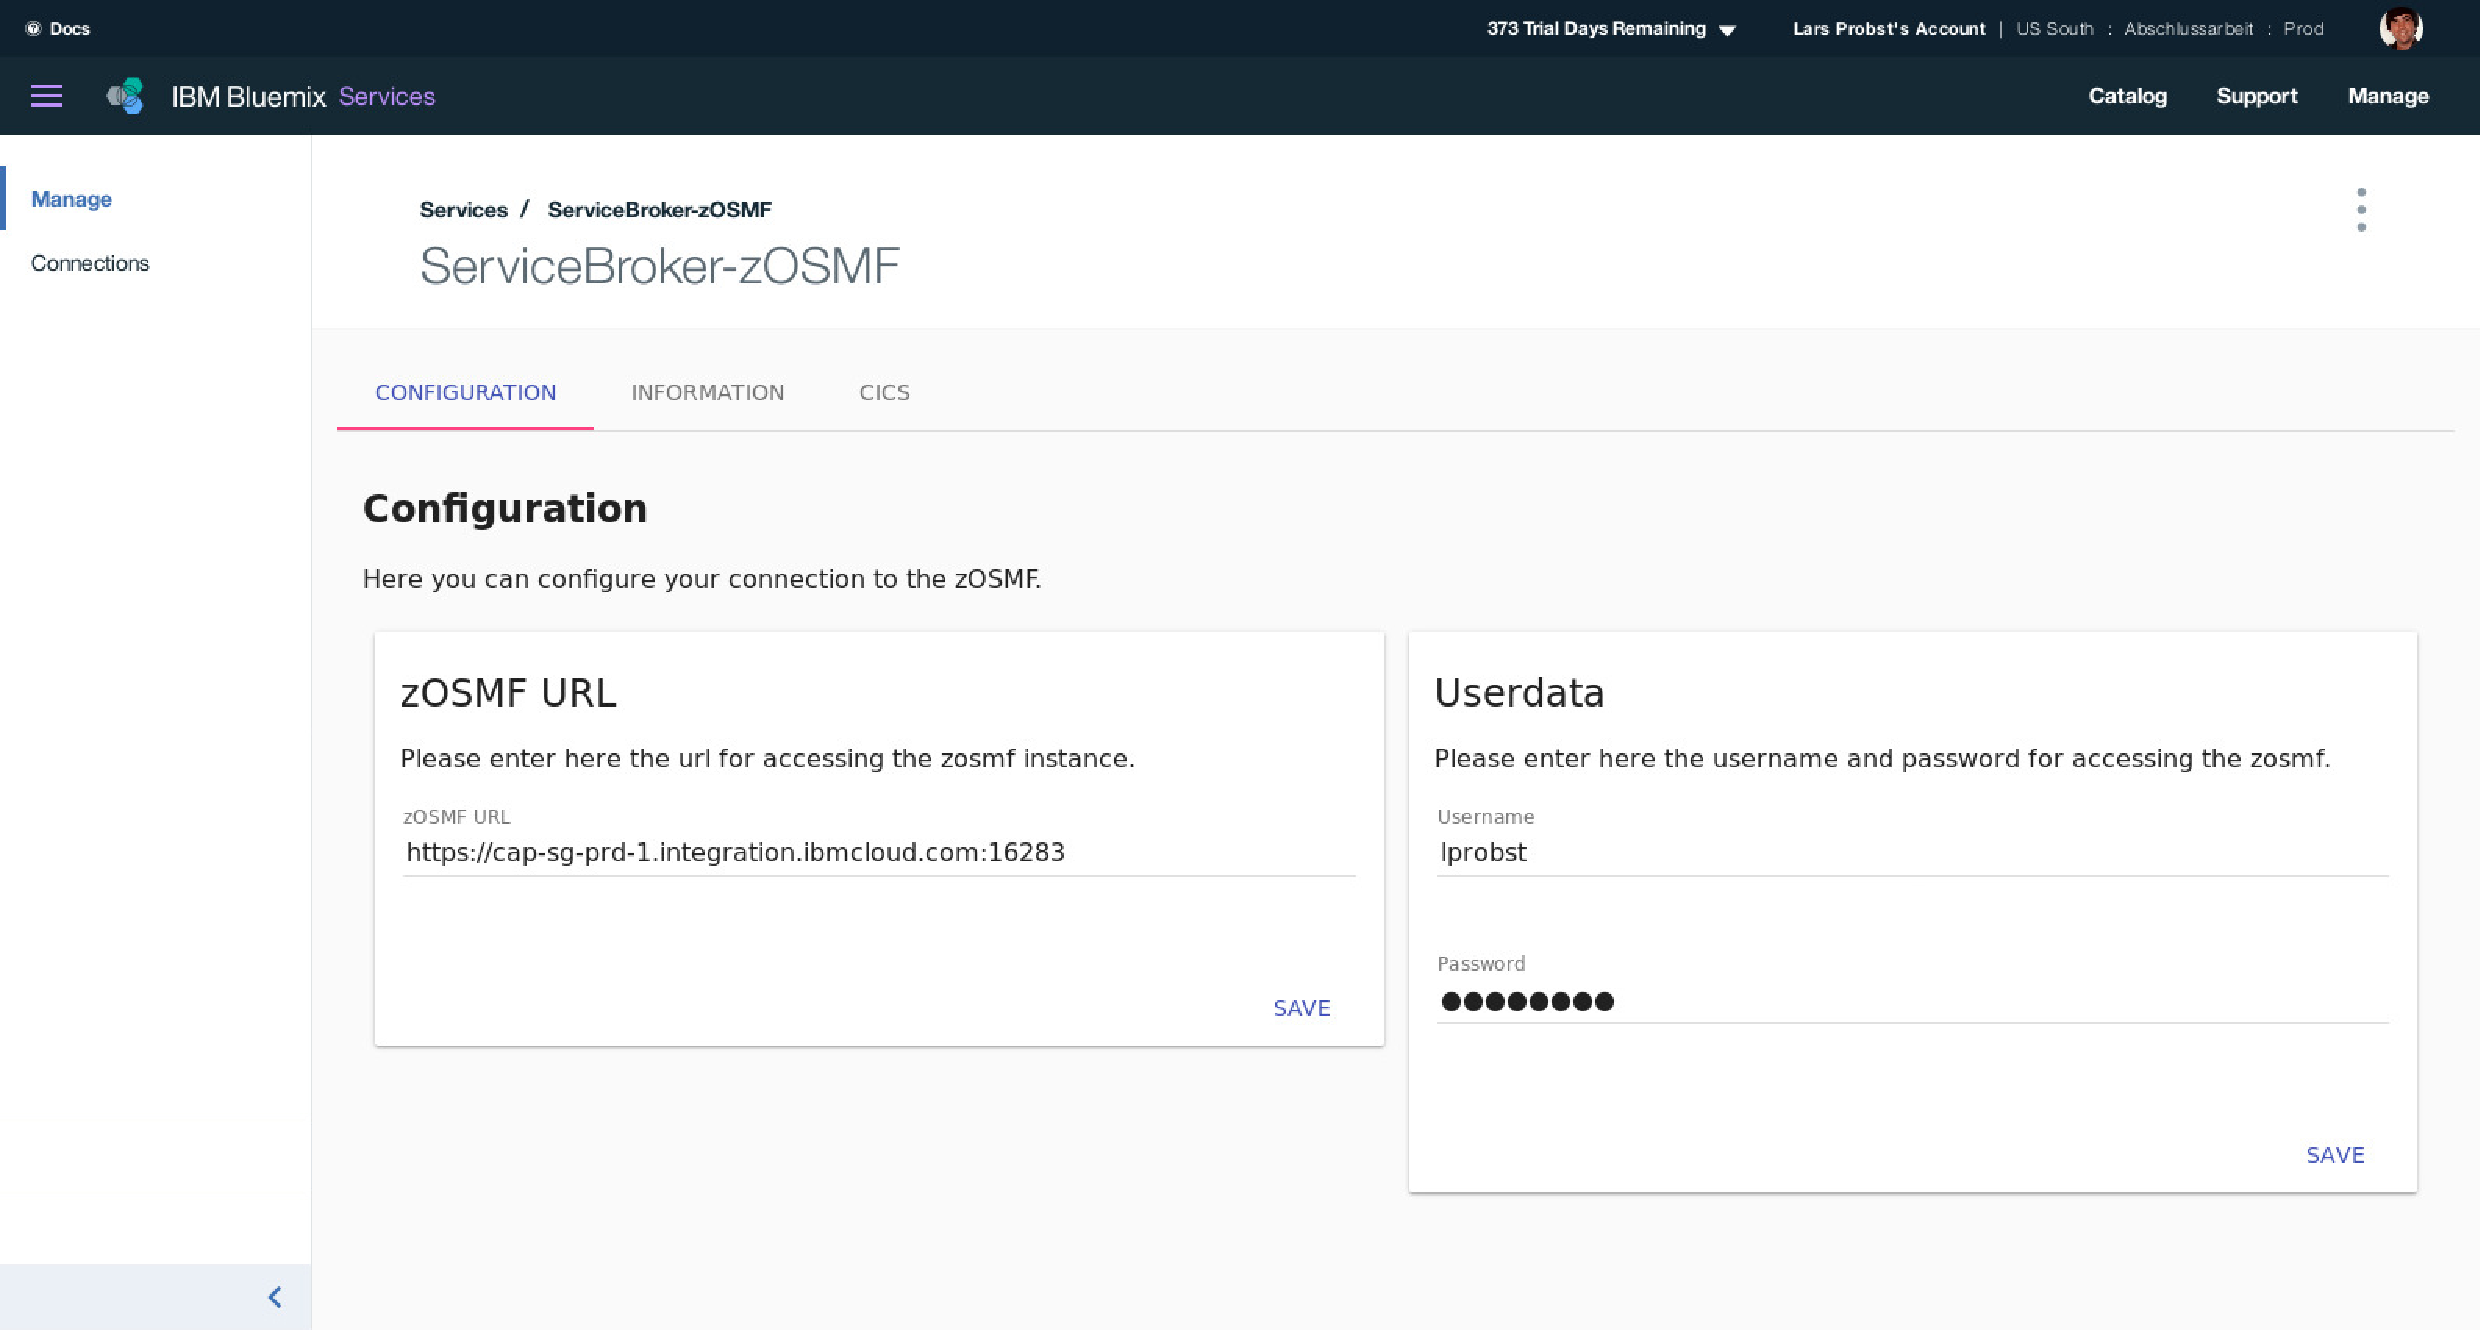
\includegraphics[scale=0.31]{images/kapitel_3/servicebroker_configuration.pdf}
  \caption{Konfiguration des Service Brokers}
  \label{fig:servicebroker_configuration}
\end{figure}

Dort wird im Bereich \path{zOSMF URL} die URL der zOSMF Instanz eingetragen, die im Secure Gateway hinterlegt ist. Dies
ist wichtig, damit der Service Broker das RESTFul-Interface aufrufen kann.

Damit der Service Broker Jobs in zOSMF ausführen kann, muss dieser sich am Interface authentifizieren. Dazu wird im Bereich
\path{Userdata} der Benutzername und das zugehörige Passwort eines zOSMF-Benutzers eingetragen, welcher über genügend
Rechte verfügt um Service Templates auszuführen.

Mit jeweils einem Klick auf \path{Save}, werden die Informationen dauerhaft im Service Broker gespeichert. Nun kann
getestet werden, ob die Eingabe der Daten korrekt war. Dazu wird der Reiter \path{Information} geöffnet. Dort sollten nun
Informationen über die zOSMF Instanz sowie der z/OS Version angezeigt werden.

Über den Reiter \path{CICS} können alle CICS-Regionen angezeigt, gestoppt oder gestartet werden oder auch neue
hinzugefügt werden. Außerdem können, nach einem Klick auf eine CICS-Runtime, Informationen über diese angezeigt werden.

Die Einrichtung des Service Brokers ist somit abgeschlossen und die wichtigsten Informationen sind bekannt.

\subsection{Einrichten der Toolchain}
\label{subsec:einrichten_der_toolchain}
Der Service Broker ist nun eingerichtet und somit können CICS-Regionen auf dem Mainframe bereitgestellt werden. Im folgenden
soll eine Toolchain in Bluemix eingerichtet werden, die es dem Entwickler ermöglicht, aus der Cloud heraus eine Anwendung
auf eine CICS-Region zu installieren.

Dazu wird das Dashboard von Bluemix geöffnet und anschließend über das Menü am linken oberen Rand der Punkt \path{Services}
und anschließend \path{DevOps} ausgewählt. Nun öffnet sich der Bluemix Bereich DevOps. In diesem ist es neben der Verwaltung
von Toolchains möglich, \textit{Pipelines} und \textit{Services} einzurichten.

Mit einem Klick auf \path{Toolchains} öffnet sich die Konfiguration dieser. Dort kann mit dem Button
\path{Toolchain erstellen} eine neue erstellt werden. Im sich öffnenden Fenster kann entweder eine Vorlage der zahlreichen
vorkonfigurierten Toolchains genutzt, oder eine eigene erstellt werden.

In diesem Beispiel wird die Vorlage mit dem Namen \path{Einfache Cloud Foundry-Toolchain (v2)} genutzt, da so ein
Git-Repository mitangelegt wird. Durch die Auswahl der Vorlage gelangt man in die Konfigurationsansicht. Siehe dazu
Abbildung \ref{fig:toolchain_konfiguration} auf Seite \pageref{fig:toolchain_konfiguration}.

\begin{figure}[h]
  \centering
    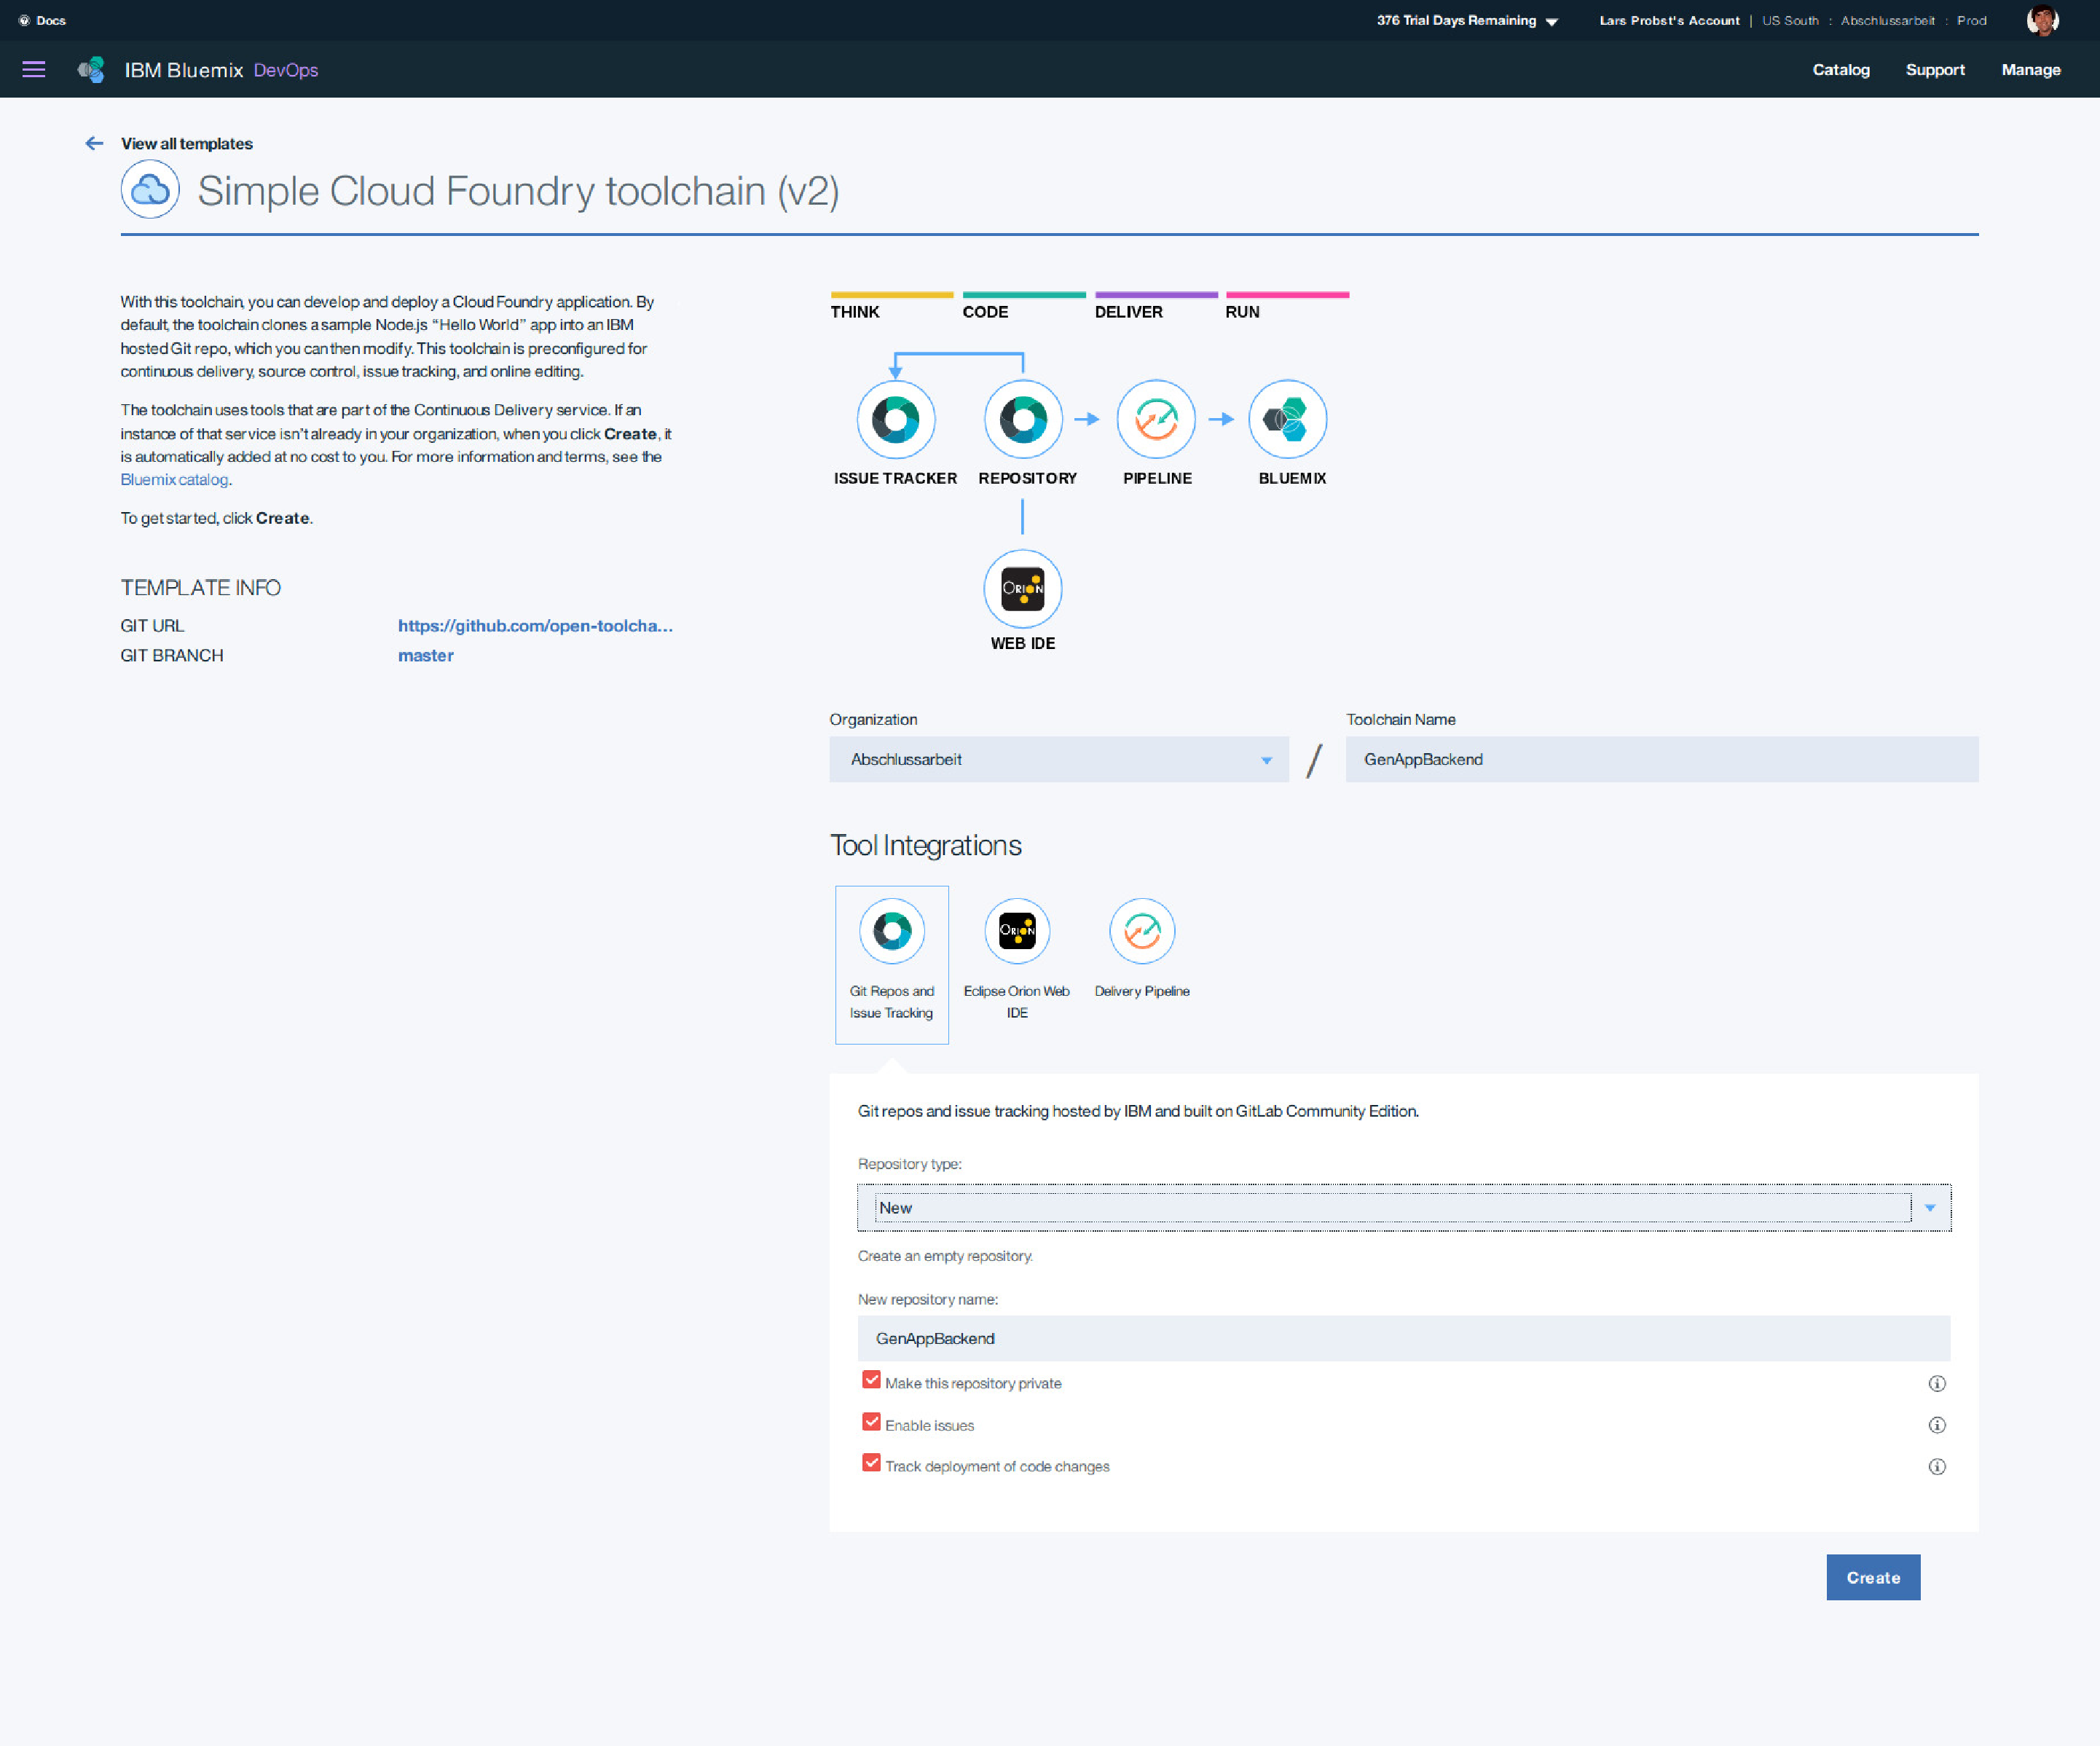
\includegraphics[scale=0.28]{images/kapitel_3/toolchain_konfiguration.pdf}
  \caption{Konfiguration der Toolchain}
  \label{fig:toolchain_konfiguration}
\end{figure}

Wie in der Abbildung zu sehen wurde als \textit{Repository type} \path{New} ausgewählt, damit ein neues, leeres
Git-Repositroy angelegt wird, in das der Quellcode gepushed werden kann. Außerdem wurde das Repository als \path{Private}
markiert und der Name \path{GenAppBackend} gewählt.

Über \path{Create} wird die Toolchain angelegt und steht ab sofort zur Verfügung. Allerdings ist diese noch nicht mit dem
Mainframe oder einer CICS-Region verbunden.

Im Anschluss öffnet sich die Übersicht der eingerichteten Toolchain. Dort kann das Git-Repository verwaltet, die
Web-IDE genutzt oder die Build Pipeline verwaltet werden.

Da es aktuell noch nicht möglich ist, direkt einen Mainframe oder eine CICS-Region über den Secure Gateway anzugeben und
keine eigenen Services zur Toolchain hinzugefügt werden können, muss diese Verbindung und die Installation des Artefaktes
noch händisch gemacht werden. Siehe mehr dazu im Kapitel \textit{Ausblick} \ref{sec:erweiterung_der_toolchain} auf Seite
\pageref{sec:erweiterung_der_toolchain}.

Die Einrichtung der Toolchain ist hiermit vorerst beendet, da die \path{DEPLOY}-Stage für jede CICS-Region anders
konfiguriert werden muss. Mehr dazu in Kapitel \ref{cha:prototypische_anwendung}, bei der Umsetzung der prototypischen
Anwendung.

\subsection{Einrichten von UCD}
Mit der Einrichtung der Toolchain in Kapitel \ref{subsec:einrichten_der_toolchain} auf Seite
\pageref{subsec:einrichten_der_toolchain} ist eine der zwei benötigten Funktionen umgesetzt, ein Artefakt aus dem Quellcode
zu bauen und auf dem Mainframe zu installieren.

Die zweite Funktion, die Installation über UCD, soll in diesem Kapitel beschrieben werden. Der Workflow des Software
Service Templates in zOSMF, der CICS-Regionen registriert, fügt diese nach erfolgreicher Einrichtung automatisch direkt
in UCD ein. Dies hat zur Folge, dass der Aufruf von UCD eine Übersicht aller eingerichteten CICS-Regionen anzeigt. Siehe
dazu Abbildung \ref{fig:ucd_overview} auf Seite \pageref{fig:ucd_overview}.

\begin{figure}[h]
  \centering
    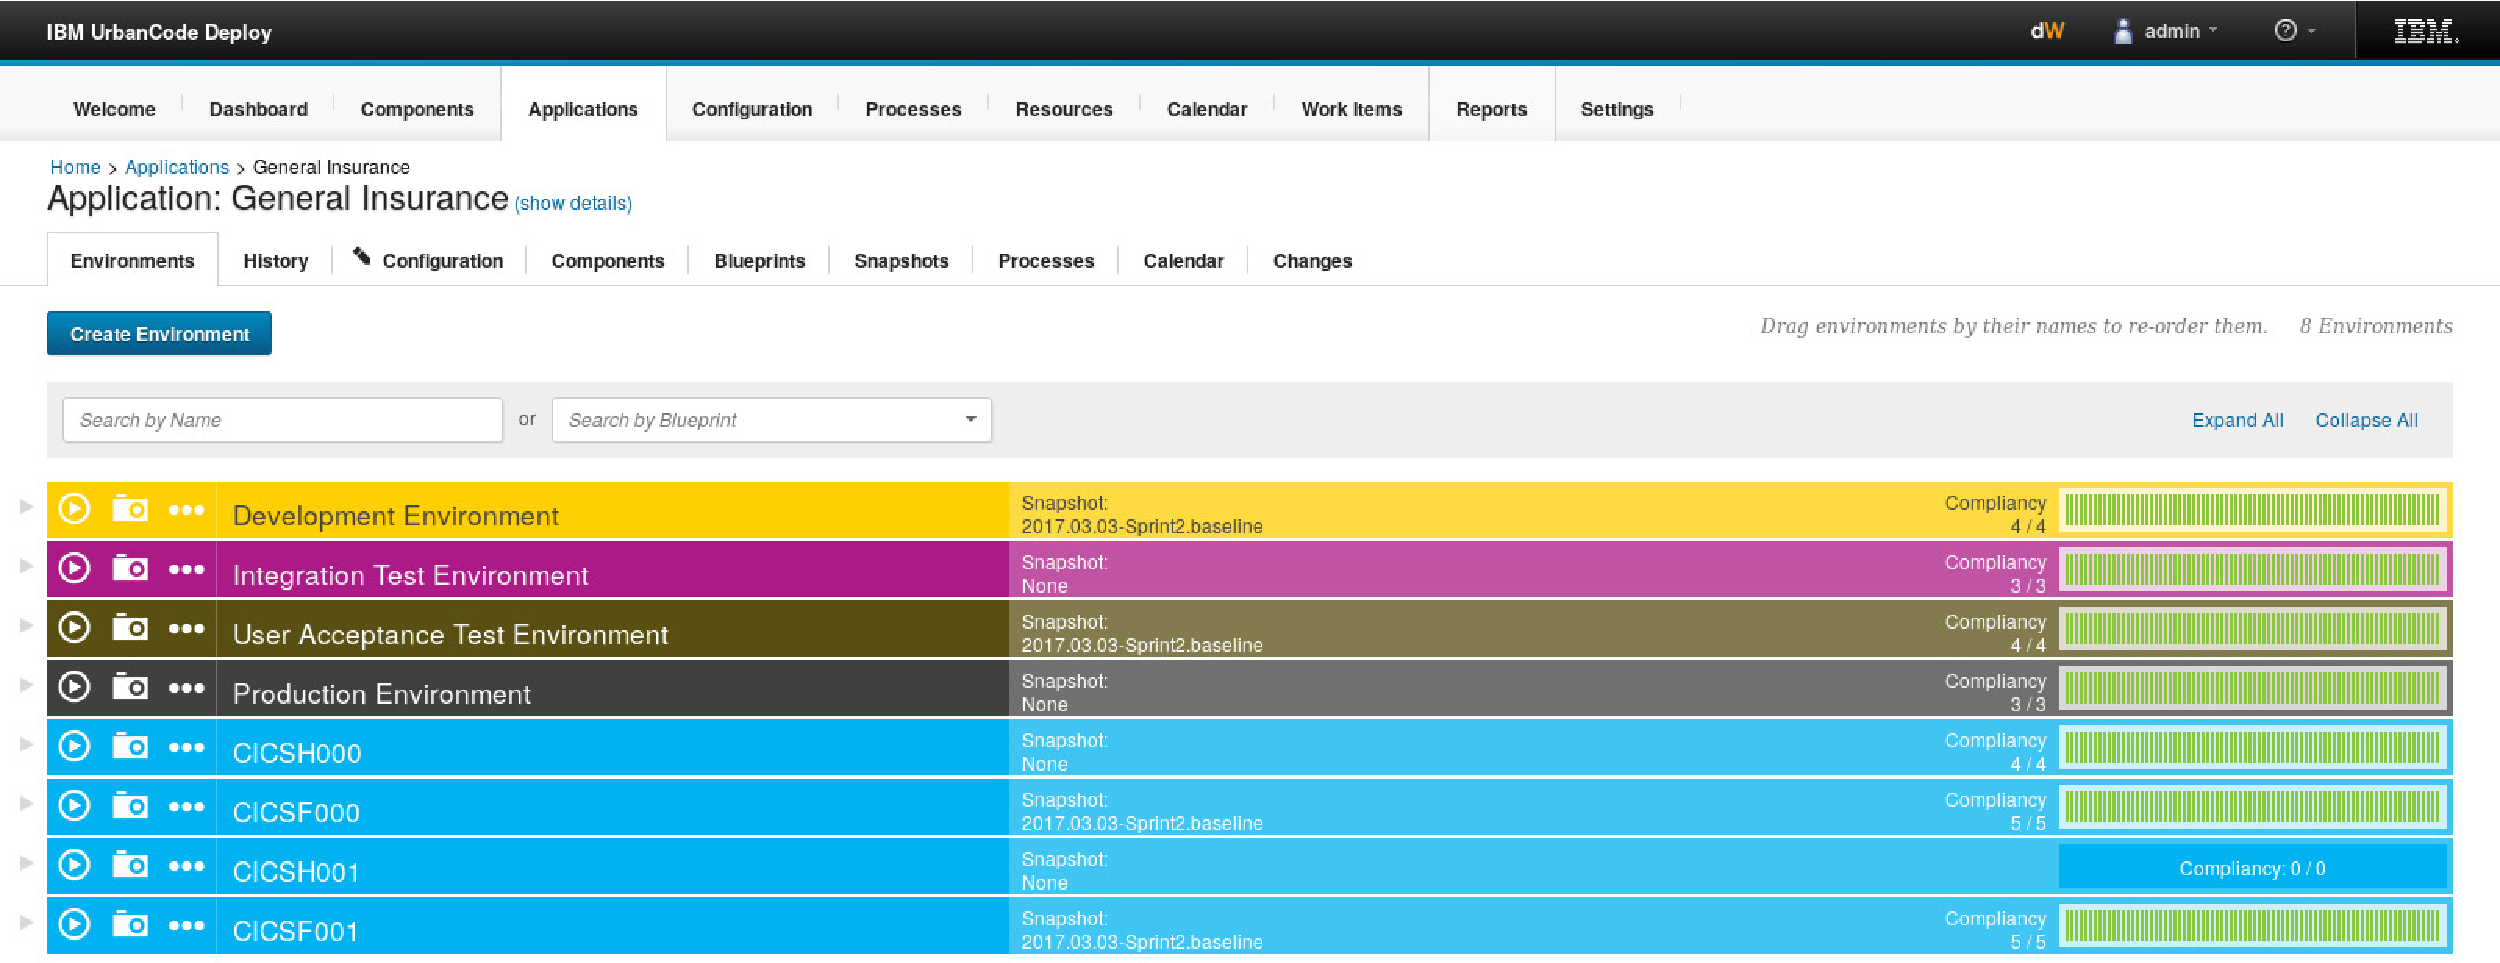
\includegraphics[scale=0.31]{images/kapitel_3/ucd_overview.pdf}
  \caption{Übersicht der Systeme in UCD}
  \label{fig:ucd_overview}
\end{figure}

Es muss lediglich eine Applikation im UCD eingerichtet werden. Die Einrichtung einer Anwendung in UCD ist relativ aufwendig
und kann im IBM Knowledge Center\footnote{https://ibm.co/2uSkr5M} nachgelesen werden. Dort wird die Einrichtung mit 2-3
Stunden angegeben.

Ist die Einrichtung allerdings erfolgreich fertiggestellt, kann, wie in Abbildung \ref{fig:ucd_start} auf Seite
\pageref{fig:ucd_start} zu sehen, eine CICS-Region mit der gewünschten Anwendung bestückt werden.

\begin{figure}[h]
  \centering
    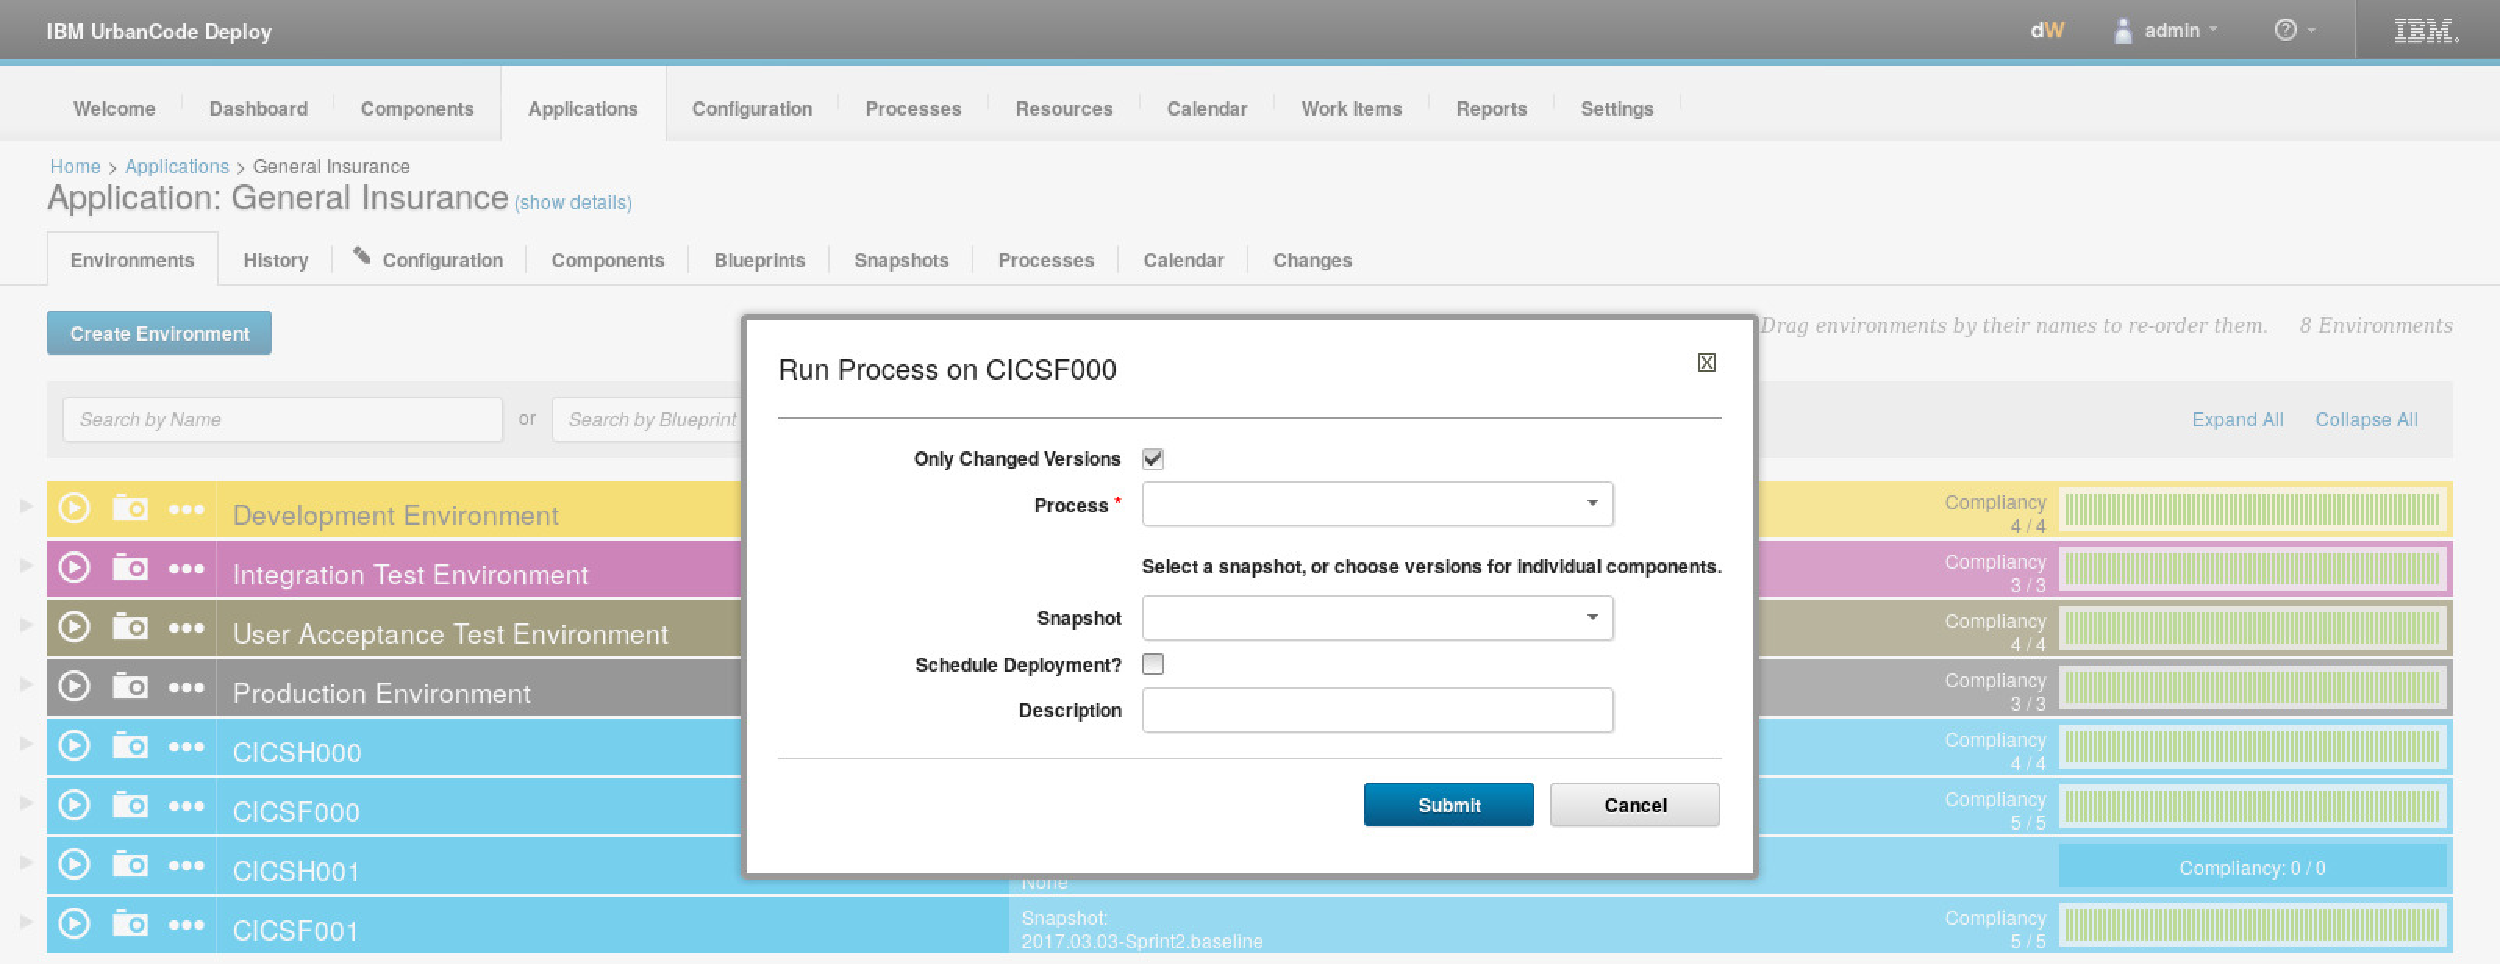
\includegraphics[scale=0.31]{images/kapitel_3/ucd_start.pdf}
  \caption{Start eines Deployments}
  \label{fig:ucd_start}
\end{figure}

Nach dem Start der Aufgabe sollte es lediglich wenige Minuten dauern, bis die Anwendung erfolgreich auf der ausgewählten
CICS-Region zur Verfügung steht.
\section{Abschluss}
Da die Hybrid-Cloud-Architektur nun erfolgreich konzipiert und aufgebaut ist, kann diese getestet werden.

Der Aufbau eines solchen Tests für die Architektur ist allerdings relativ aufwendig und aufgrund der verteilten Systeme,
die teilweise keine Kommunikation zu anderen Bestandteilen haben, nicht aussagekräftig und wird deshalb nicht realisiert.

Allerdings kann die vorliegende Architektur durch eine prototypische Implementierung getestet werden. Diese Umsetzung wird
in Kapitel \ref{cha:prototypische_anwendung} ab Seite \pageref{cha:prototypische_anwendung} realisiert.
\chapter{Prototypische Anwendung}
\label{cha:prototypische_anwendung}

Im folgenden Kapitel wird eine Applikation entwickelt, welche die in Kapitel \ref{cha:hybrid_cloud_architektur} ab Seite
\pageref{cha:hybrid_cloud_architektur} erarbeitete Hybrid-Cloud-Architektur prototypisch implementiert.

Dafür wird ein Web-Frontend erstellt, welches die in einer Datenbank vorliegenden Informationen visualisiert. Bei den
Daten handelt es sich einerseits um statische Werte wie Vorname, Nachname, usw. als auch um dynamische Werte wie zum
Beispiel ein Kundenwert, der in einem Diagramm dargestellt werden soll.

Zur Umsetzung wird neben einer Laufzeitumgebung für das Frontend auch der Service Text\-2Speech in Bluemix eingerichtet.
Die erstellte Laufzeitumgebung und der Service werden im Anschluss miteinander verbunden, damit diese Daten über die
VCAP-Variaben austauschen können.

Den Zugriff auf die Daten in der Datenbank ermöglicht eine COBOL-Anwendung, welche nicht näher beschrieben oder definiert
ist. Dies bedeutet, dass es keine Informationen über Schnittstellen oder der genaue Funktionsweise der Anwendung gibt.
Eine Analyse der Schnittstellen und Funktionen erfolgt durch das Tool \textit{IBM Application Discovery}.

Nachdem die Schnittstellen der COBOL-Anwendung definiert sind, wird ein Java-Wrapper geschrieben, welcher eine
REST-Schnittstelle zur Verfügung stellt. Diese kann genutzt werden, um Daten aus der Datenbank über die COBOL-Anwendung
zu erhalten. Die Kommunikation zwischen dem Java-Wrapper und COBOL-Anwendung erfolgt durch die Schnittstelle \textit{WOLA}.

Da die COBOL-Anwendung nicht alle Informationen aus der Datenbank liefert, wird zusätzlich der DB2 Rest Service sowie ein
Machine Learning (Watson)-Service genutzt.

Wie in \cite{online_einleitung_app} zu lesen, spielt für viele Firmen neben einer vernünftigen Webseite auch eine
Smartphone-App eine immer wichtigere Rolle. Aus diesem Grund wird im nächsten Schritt sowohl eine Android- als auch eine
iOS-App erstellt.

Diese stellen ebenfalls die Informationen aus der Datenbank dar und sollen sich für den leichten Umstieg hinsichtlich
Funktion und Design, wenn überhaupt, nur gering von dem Web-Frontend unterscheiden.

Die Kommunikation zwischen Frontend, Android- und iOS-App und dem Backend auf dem Mainframe erfolgt durch
den Secure Gateway-Service in Bluemix.

Eine grobe, schematische Übersicht über die zu implementierende Anwendung ist in Abbildung \ref{fig:architektur_clouduebersicht}
auf der Seite \pageref{fig:architektur_clouduebersicht} zu sehen.

\begin{figure}[h]
  \centering
    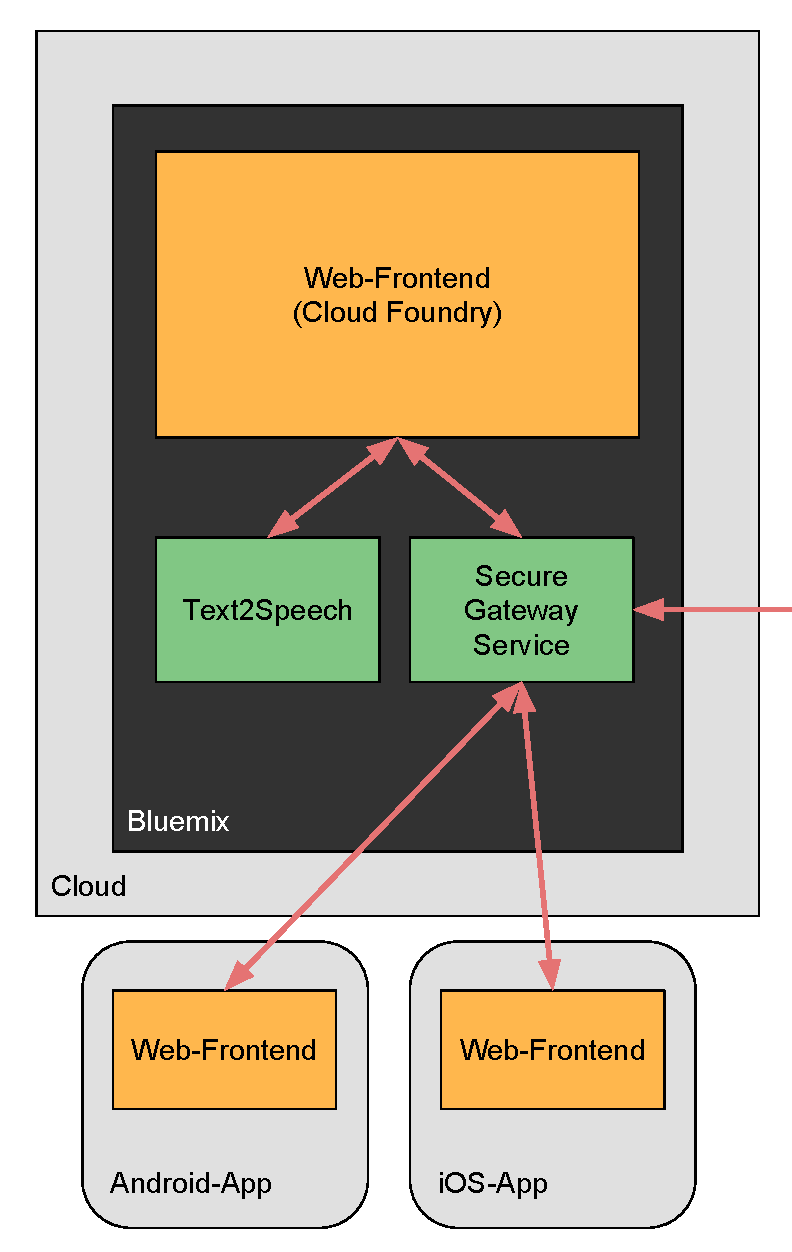
\includegraphics[scale=0.5]{images/kapitel_4/architektur_clouduebersicht.pdf}
  \caption{Grobe Übersicht über die Prototypische Anwendung}
  \label{fig:architektur_clouduebersicht}
\end{figure}
\section{Analyse}

\subsection{Architektur}
Für Webseiten gibt es zahlreiche Frameworks, welche wiederum zahlreiche Architekturen umsetzen. Das MVC-Pattern hat sich
in der Vergangenheit großflächig durchgesetzt (siehe dazu \cite{book_prototypischeanwendung_mvc}) und wird in diesem Beispiel
verwendet.

Ein großer Vertreter des MVC-Patterns ist AngularJS. Neben der schnellen Einarbeitung ist AngularJS sehr mächtig und es
kann eine Single-Page Applications (kurz SPA) geschrieben werden. Bei diesem Web-Frontend soll es sich um eine SPA handeln.

Auf der Backendseite wird ein REST-Interface entwickelt, welches die eingehenden Anfragen an die COBOL-Anwendung weiterleitet.
Da seit kurzem ein WebSphere-Liberty-Profile für CICS existiert und dieses neben vielen Vorteilen gegenüber anderen
Application-Servern sich noch großer Beliebtheit erfreut (siehe \cite{online_prototypischeanwendung_cicsliberty}),
wird das REST-Interface in Java entwickelt, um das WebSphere-Liberty-Profile zu nutzen.

Um einen weiteren Vorteil der Hybrid-Cloud-Architektur aufzuzeigen, soll außerdem die REST-Schnittstelle der vorliegenden
DB2-Instanz genutzt werden. Dazu wird ein so genannter Service eingerichtet, der die Daten zurückgeben kann, welche die
COBOL-\-Anwendung standardmäßig nicht zurückgeben kann.

\subsection{Services}
Um einen Mehrwert der Cloud aufzuzeigen, soll das Web-Frontend durch einen Cloud-Service aufgewertet werden. Dabei stehen
neben analytischen Services in IBM Bluemix auch Watson Services zur Verfügung.

Da die Anzahl der Daten in der Demo zu gering ist, entsteht kein großer Mehrwert durch analytische Services. Es wird
deshalb der Watson Service Text2Speech eingebaut. Dieser wandelt geschriebenen Text in Sprache um. Bei der Umwandlung
entsteht eine Audio-Datei, welche in gängigen Webbrowsern abgespielt werden kann.

Der Service wird immer dann verwendet, wenn das Backend Daten an das Web-Frontent zurückgegeben hat.

\subsection{Runtime}
Um das Web-Frontend auf Bluemix laufen zu lassen, wird eine Runtime benötigt. Zur Auswahl stehen neben Cloud Foundry auch
ein Docker-Container und der Service Object Storage.

Der Object Storage Service speichert Dateien online. Diese können dann mittels statischer URL aufgerufen werden. Um eine
AngularJS-Webseite damit zu hosten, müssen alle Dateien hochgeladen und anschließend referenziert werden. Das
ist relativ mühsam, da eine Referenzierung in der lokalen IDE erst nach dem ersten Upload möglich ist.

Alternativ kann in einem Docker Container ein Webserver laufen, welcher das Web-Frontend statisch zurückliefert.

In diesem Beispiel wird ein Cloud Foundry Container verwendet. Dieser hat den Vorteil, dass er Zugriff auf die
Cloud Foundry Environment-Variablen\footnote{https://docs.run.pivotal.io/devguide/deploy-apps/environment-variable.html}
(kurz cf env) in Bluemix hat, welche die Zugriffsinformationen für die verschiedensten Services hält.

Im Cloud Foundry Container läuft ein Express Server unter NodeJS. Dies erleichtert unter anderem den Zugriff auf die
VCAP-Variablen, welche sich in den cf env Variablen befinden.

Das Backend wird in einem WebSphere-Liberty installiert, welches in einem CICS läuft. Es wird dabei das
WebSphere-Liberty-Profile genutzt.

\subsection{Smartphone App}
Eine Möglichkeit die Smartphone-Apps zu erstellen ist es, sie nativ in der jeweiligen Sprache zu schreiben und auf dem
Smartphone zu installieren. Das Problem ist, dass das jeweilige Smartphone dann eine VPN-Verbindung zum Mainframe-Netz
besitzen muss, um auf das Backend zugreifen zu können. Das Öffnen des Mainframe-Netzwerkes für mehrere Endgeräte kann
allerdings zu einer große Sicherheitslücke führen.

Alternativ kann auch der Secure Gateway genutzt werden, welcher schon eine Verbindung in das Rechenzentrum hat. Dann
müsste bei einer Änderung des Secure Gateways allerdings immer ein Update für die entsprechenden Applikationen zur
Verfügung gestellt werden.

Auch könnte eine WebViewer-App entwickelt werden. Dabei wird das Web-Frontend in einen Web-Container geladen und dem
Nutzer suggeriert, dass es sich um eine reale App handelt. Sofern die Webseite so gestaltet ist wie eine App, fällt der
Unterschied in den meisten Fällen nicht auf.

In diesem Beispiel wird eine WebViewer-App entwickelt, da so dass schon geschriebene Web-Frontend wiederverwendet werden
kann und sich dadurch die Entwicklungszeit und Wartung deutlich verkürzt.

\subsection{Frontend-Design}
Genau wie bei der Architektur einer Anwendung gibt es auch im Bereich Design einer Webseite zahlreiche Frameworks. Nach
t3n \cite{online_prototypischeanwendung_cssframework} ist \path{Bootstrap} das wohl bekannteste CSS Framework.

Da in diesem Beispiel allerdings auch Smartphone-Apps erstellt werden, muss das Web-Frontend eine große Ähnlichkeit zu
diesen Apps haben. Aus diesem Grund wird Googles Material Design verwendet. Für AngularJS gibt es das Angular
Material Plugin\footnote{https://material.angularjs.org/latest}, welches die Material-Design
Spezifikationen\footnote{https://material.io/guidelines} von Google umsetzt.

\subsection{Bestehende Anwendung}
Um zu demonstrieren, wie ein neu geschriebenes Web-Frontend in der Cloud mit einer Anwendung auf einem Mainframe
kommunizieren kann, wird eine schon bestehende Anwendung benötigt, welche den Bestand einer Firma repräsentieren soll.

Hierfür wird eine einfach gehaltene COBOL-Anwendung verwendet, welche Daten in eine Datenbank schreiben, diese auslesen
und verändern kann. Im folgenden \path{GenApp} genannt.

Die Schnittstellen und genauen Funktionen der GenApp sind allerdings nicht bekannt und müssen in weiteren Schritten
analysiert werden.

\subsection{Qualitätssicherung}
Damit beim regelmäßigen Bau des Quellcodes durch die Bluemix Toolchain bzw. durch UCD immer die richtige Qualität gewahrt
werden kann, sollen für das Web-Frontend, das Java-Backend und die Smartphone-Apps automatisierte Tests geschrieben werden.

Dabei wird das Web-Frontend durch PhantomJS, einem Headless Browser, getestet. Das Java-Backend und die Android-App jeweils
mit JUnit-Tests.
\section{Vorbereitung}
In diesem Abschnitt werden Vorbereitungen für die Entwicklung auf Bluemix und für Cloud Foundry Container getroffen. Dabei
werden unter anderem Programme installiert und eingerichtet.

\subsection{Git}
Um mit Git-Repositorys arbeiten zu können, wird ein lokaler Git-Client benötigt. Dieser kann unter Ubuntu mit folgenden Befehlen
installiert und eingerichtet werden.

\begin{lstlisting}[language=bash, caption=Installieren von Git, label=Installieren von Git]
   $ sudo apt-get update
   $ sudo apt-get install git
\end{lstlisting}

Eine Windows- und MacOS-Installer kann auf der Webseite von Git heruntergeladen werden\footnote{https://git-scm.com}.

\subsection{IBM Application Discovery}
Um die COBOL-Anwendung analysieren zu können wird das Tool IBM Application Discovery genutzt. Die Installation des Tools
kann auf zwei Arten geschehen.

\begin{itemize}
    \item{Manuelle Installation des Servers und der Clients}
    \item{Nutzen einer Virtual Machine}
\end{itemize}

Da die manuelle Installation des Servers und der Clients recht langwierig ist und in der
Installationsanleitung\footnote{https://www.ibm.com/support/knowledgecenter/en/SSRR9Q} nachgelesen werden kann, wird hier
kurz auf die Nutzung der Virtual Machine eingegangen.

Um die Virtual Maschine nutzen zu können, wird ein Tool benötigt um diese abzuspielen. Eine Möglichkeit ist das Programm
\path{VM VirtualBox}\footnote{https://www.virtualbox.org} von Oracle.

Nach der Installation von VM VirtualBox muss die Virtual Mashine von IBM Application Discovery heruntergeladen werden.
Die Dateien stehen im IBM
Repository\footnote{http://ausgsa.ibm.com/projects/r/rational\_mktengr\_team/EM/EZSourceSoftwareAndDocs\\/VMImage2016-10-05}
zur Verfügung.

Nach dem Download der 19 Teilarchiv-Dateien müssen diese durch einen Archivmanager zusammengefügt und die \path{.vmx}-Datei
extrahiert werden.

Im letzten Schritt wird die \path{.vmx}-Datei als Festplatte in VM VirtualBox hinzugefügt und gestartet.

In der gestarteten Virtual Mashine befindet sich sowohl der IBM Application Discovery Server als auch ein Client, mit dem
die Anwendungen analysiert werden können.
\section{Umsetzung}
Die Abbildung \ref{fig:architektur_gesamtuebersicht} auf Seite \pageref{fig:architektur_gesamtuebersicht} zeigt neben der
schon implementierten Hybrid-Cloud-Architektur (leicht ausgewaschene Farben) die Übersicht der Zielimplementierung der
Anwendung (rote Umrandung). In dieser ist zu sehen, dass in Bluemix neben einer Cloud Foundry Runtime auch drei Services
instanziiert werden. Außerhalb von Bluemix werden zwei Smartphone-Apps entwickelt. Eine für Android und eine für iOS.

Im Backend (Mainframe) wird um die GenApp ein Java-Wrapper geschrieben, welcher die Anfragen aus der Cloud weitergibt und
die Daten aus einer DB2 holt. Der Java-Wrapper wird in einem WebSphere Liberty Profile laufen.

Außerdem wird es in der DB2 einen Service geben, der Daten direkt über eine REST-Schnittstelle zur Verfügung stellt. Dieser
Service wird mit einem statischen SQL-Befehl erstellt. Durch diese Schnittstelle werden Daten zurückgegeben, die durch
die COBOL-Anwendung nicht abgedeckt werden. Diese Funktion nennt sich \path{DB2 REST Service}.

In der Cloud Foundry Runtime (Web-Frontend) wird ein Ubuntu installiert, welches mit NodeJS und dem Node Package Manager
(kurz NPM) vorkonfiguriert wird. Mittles NPM wird der Express-Server nachinstalliert, der das Web-Frontend statisch
zurückliefern kann.

Das Web-Frontend ist eine AngularJS Webseite, welche mit Angular Material Design umgesetzt wird. Dabei greift es mittels
Angular-Factories auf das REST-Interface des Backends zu, um die Daten aus der Datenbank zu visualisieren.

Der Text2Speech Service wird von der Runtime direkt über die VCAP-Variablen angesprochen und erhält geschriebenen Text
von der Anwendung. Dieser wird dann in eine Audio-Datei umgewandelt, die zurückgeliefert und dann durch den Webbrowser
ausgegeben wird.

Der Secure Gateway Service ist der instanziierte Service, der wie in Kapitel \ref{subsection:secureGateway} auf Seite
\pageref{subsection:secureGateway} beschrieben eingerichtet wurde. Dieser wird mit der Cloud Foundry Runtime verbunden,
sodass die Informationen im Web-Frontend zur Verfügung stehen und eine Verbindung aufgebaut werden kann.

Der Service Broker ist der in Kapitel \ref{subsection:writeservicebroker} auf Seite \pageref{subsection:writeservicebroker}
beschriebene Service, welcher die Kommunikation zwischen Cloud und Mainframe verwaltet.

Die Smartphone-Apps erhalten jeweils ein WebView-Layout. Mit diesem kann innerhalb einer nativen App eine beliebige Webseite
dargestellt werden. Bei der dargestellten Webseite handelt es sich um das entwickelte Web-Frontend, welches vom Express-Server
ausgegeben wird. Dabei lädt das Layout die entsprechende Webseite herunter und zeigt sie dem Benutzer an.

Eine Übersicht des kompletten Quellcode zum Herunterladen gibt es in der IBM GitHub-Organisation
\path{Mainframe2020}\footnote{https://github.ibm.com/orgs/mainframe2020/dashboard}.

Der Quellcode für die einzelnen Anwendungen kann jeweils in einem öffentlichen GitHub-Projekt heruntergeladen werden. Die
Links finden sich in den jeweiligen Kapiteln.

\begin{figure}[h]
  \centering
    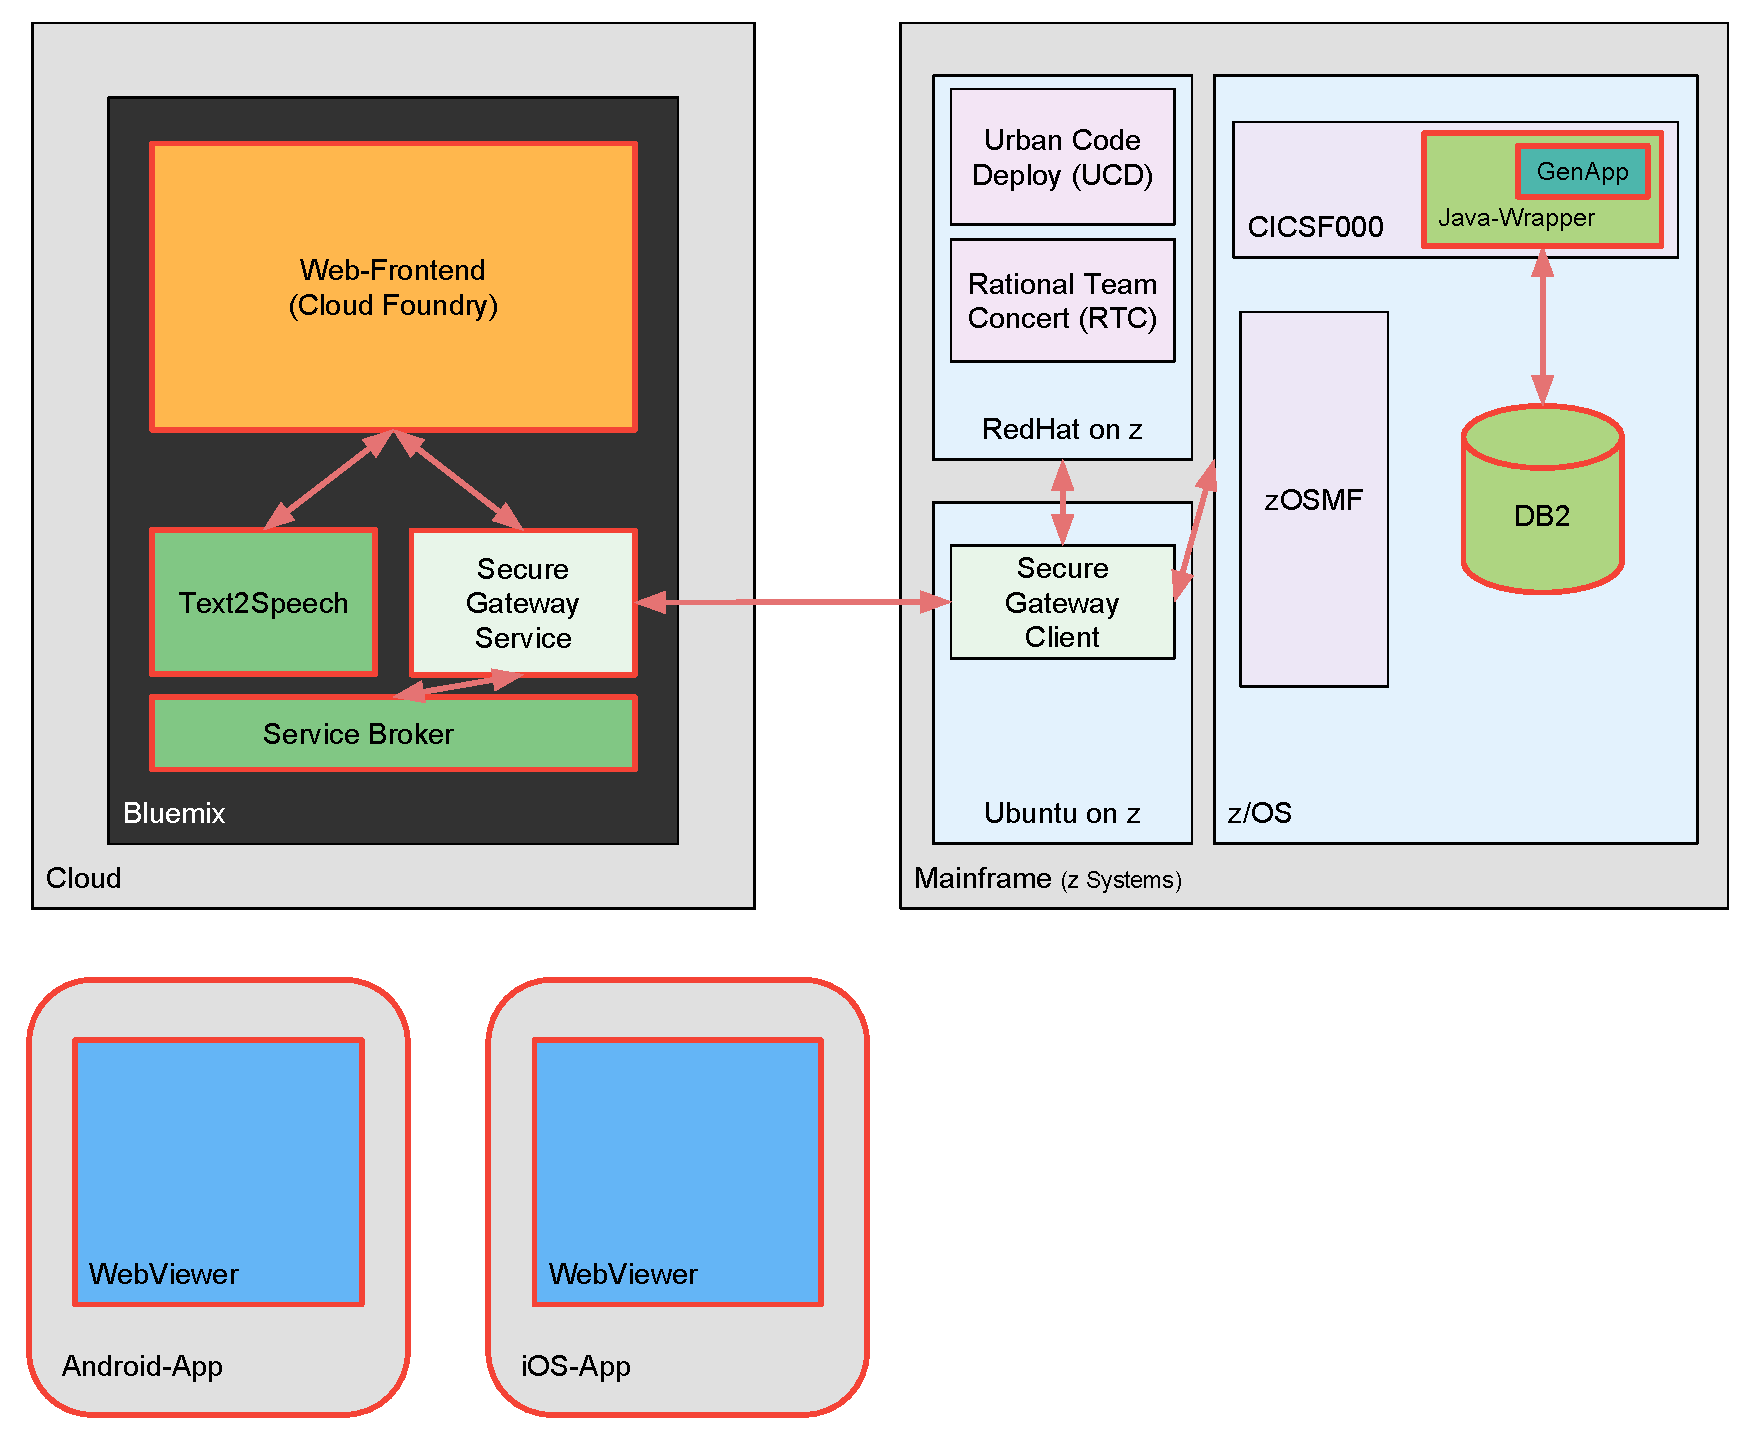
\includegraphics[scale=0.5]{images/kapitel_4/architektur_gesamtuebersicht.pdf}
  \caption{Übersicht über die Zielimplementierung}
  \label{fig:architektur_gesamtuebersicht}
\end{figure}

\subsection{COBOL-Anwendung}
Für den Start der prototypischen Implementierung der Hybrid-Cloud-Architektur wird eine vorhandene Applikation benötigt,
welche im Unternehmen eingesetzt wird oder produktiv ist.

Viele Unternehmen haben ihn ihrem Repertoire von alten aber dennoch eingesetzten Programmen durchaus COBOL-Anwendungen
in CICS-Regionen am laufen. Dies soll zum Anlass genommen werden, eine solche Anwendung ohne Anpassungen am Quellcode
für die Cloud bereit zu stellen.

In diesem Beispiel handelt es sich um die generische Applikation \path{GenApp}, für die die Oberfläche in Abbildung
\ref{fig:ibmad_map} auf Seite \pageref{fig:ibmad_map} zu sehen ist.

\begin{figure}[h]
  \centering
    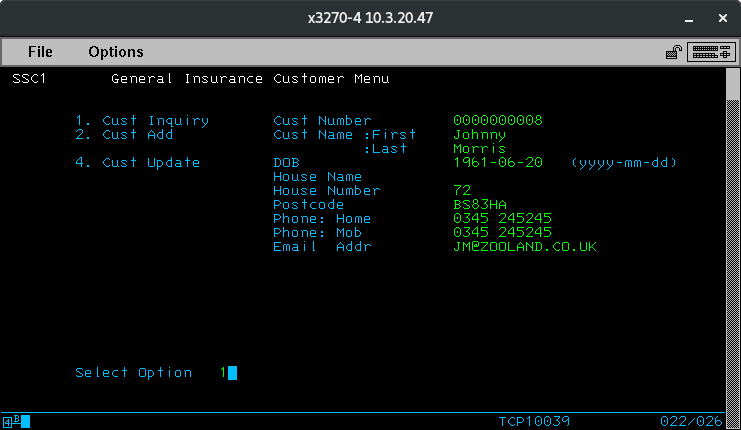
\includegraphics[scale=0.5]{images/kapitel_4/ibmad_map.png}
  \caption{Grafische Benutzeroberfläche der COBOL-Anwendung}
  \label{fig:ibmad_map}
\end{figure}

Der Transaktionsname der GenApp lautet \path{SSC1}. Durch einen Terminalaufruf des Namens in der CICS-Region wird die
Anwendung gestartet. Beim Start der Anwendung wird zuallererst die Oberfläche, die \path{BMS Map}, geladen und dem Nutzer
angezeigt.

Diese COBOL-Anwendung kann Daten aus einer Datenbank auslesen, diese bearbeiten oder neue Datensätze anlegen. Bei der
verbundenen Datenbank handelt es sich um eine DB2.

Durch eintragen einer Nummer hinter \path{Cust Number} und anschließendem ausführen der Funktion \path{Cust Inquiry}
werden die hinterlegten Informationen angezeigt. In der Abbildung sind das die Informationen des Kunden mit der Nummer
\path{8}.

Wenn Informationen überschrieben werden, können diese mit der Funktion \path{Cust Update} in der Datenbankt persistiert
werden.

Über den Parameter \path{Cust Add} und dem Hinzufügen von Informationen hinter den einzelnen Kategorien wird ein neuer
Kunde hinzugefügt.

Die Auswahl der Funktion, also \path{Cust Inquiry}, \path{ Cust Update} und \path{Cust Add}, erfolgt durch die Eingabe der
entsprechenden Zahl hinter \path{Select Option}.

Die drei Funktionen zum Verwalten der Daten, sollen dem Web-Frontend in der Cloud bereitgestellt werden. Da die genaue
Funktionsweise der Applikation jedoch nicht bekannt ist, müssen die internen Aufrufe und Übergabeparameter analysiert
werden.

\subsubsection{Analysieren der Anwendung}
Für die Analyse der COBOL-Anwendung wird das Programm \textit{IBM Application Discovery} (kurz IAD) genutzt. Eine
Übersicht der Anwendung ist in Abbildung \ref{fig:ibmad_uebersicht} auf Seite \pageref{fig:ibmad_uebersicht} zu sehen.

\begin{figure}[h]
  \centering
    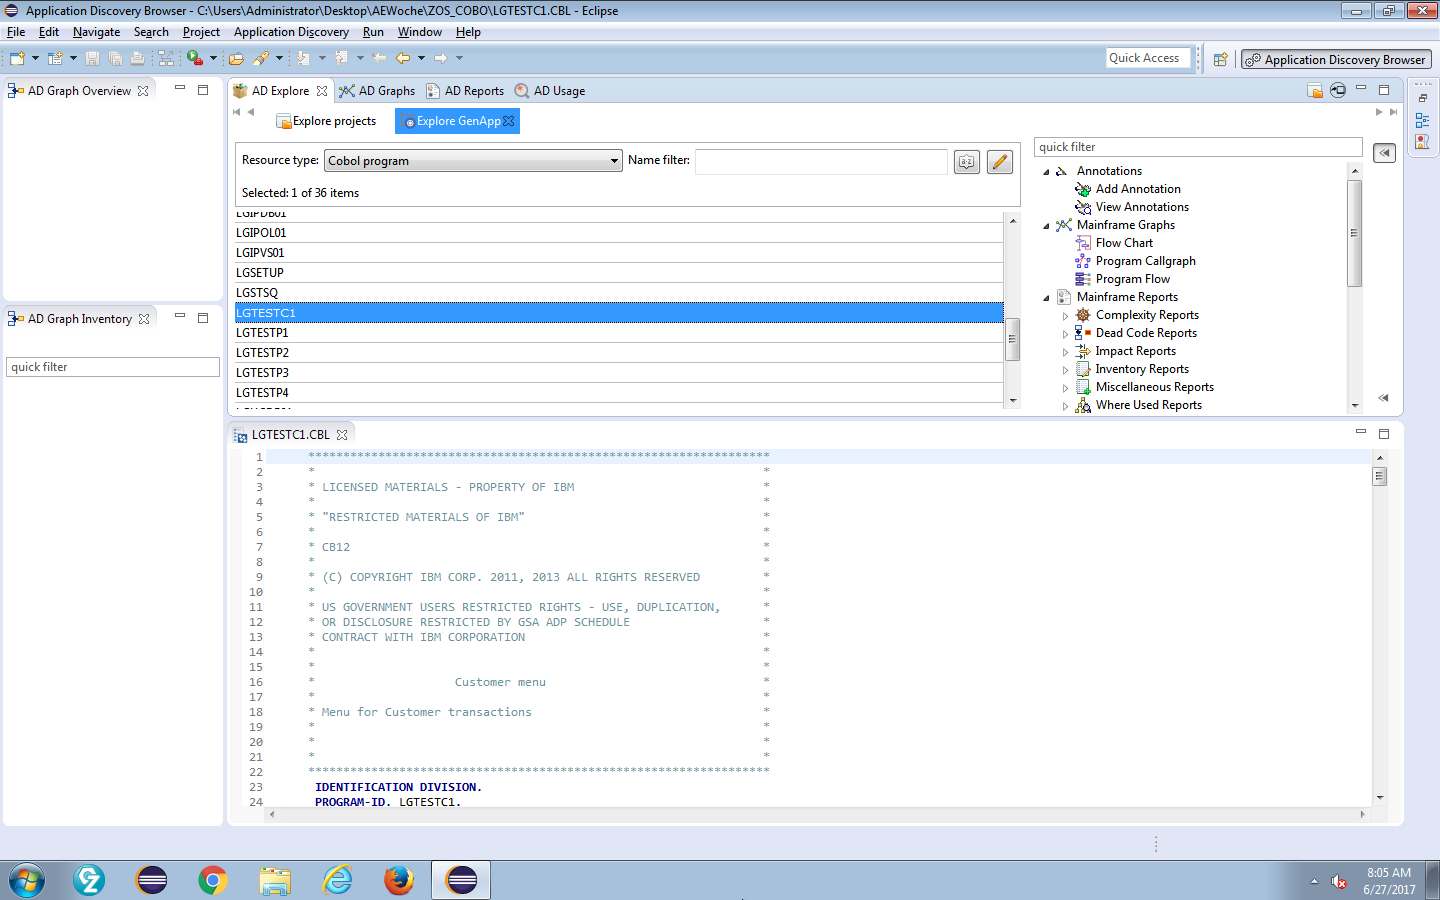
\includegraphics[scale=0.27]{images/kapitel_4/ibmad_uebersicht.png}
  \caption{Übersicht über IBM Application Discovery}
  \label{fig:ibmad_uebersicht}
\end{figure}

Dort ist zu sehen, dass \path{LGTESTC1} ausgewählt und der Quellcode ersichtlich ist. Bei diesem Teilprogramm der
Anwendung handelt es sich um das \textit{Mainprogramm} der Anwendung, welches beim Starten zuallererst aufgerufen wird.

Diese Tatsache kann durch das Vergleichen des \path{Callgraph} der Anwendung herausgefunden werden. In der Abbildung
\ref{fig:ibmad_callgraph} auf Seite \pageref{fig:ibmad_callgraph} ist zu sehen, dass der Terminalaufruf \path{SSC1}, welcher
die Anwendung startet, das Programm \path{LGTESTC1} ausführt.

Dieses Programm initialisiert dann die grafische Oberfläche der Anwendung, die SSMAP.

\begin{figure}[h]
  \centering
    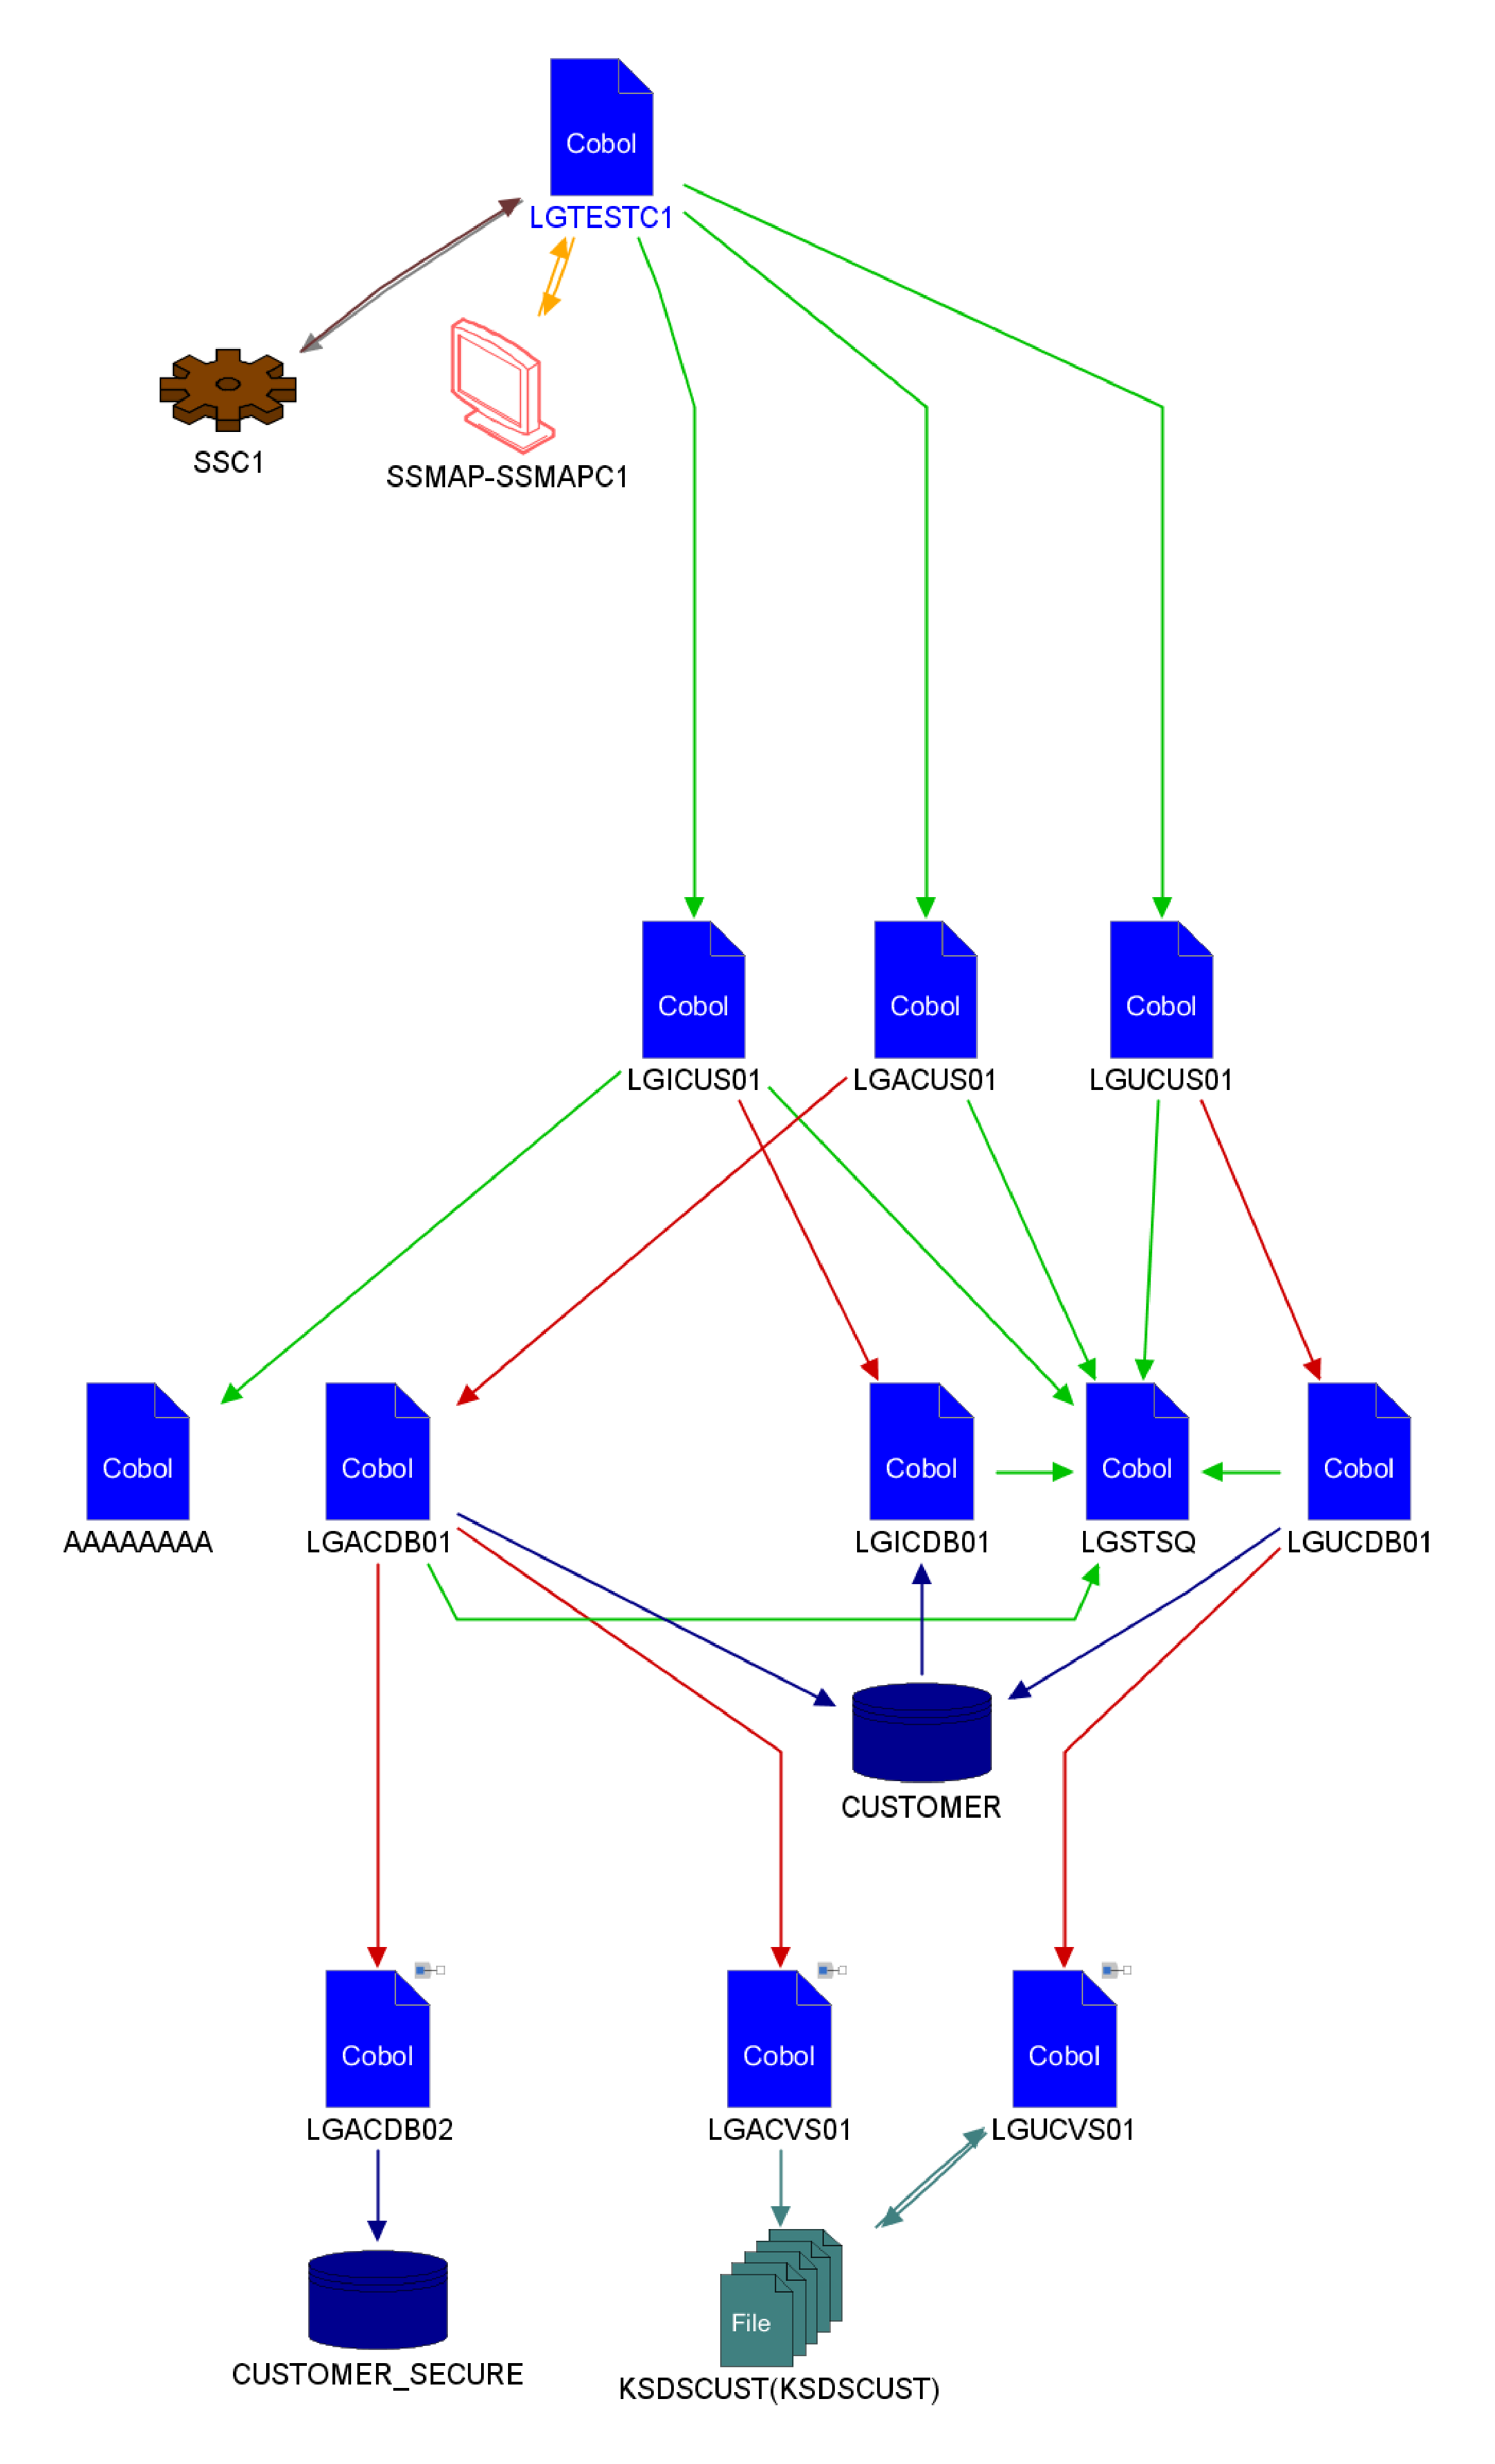
\includegraphics[scale=0.25]{images/kapitel_4/ibmad_callgraph.pdf}
  \caption{Der Callgraph der GenApp}
  \label{fig:ibmad_callgraph}
\end{figure}

Es existiert eine dauerhafte Verbindung zwischen der GUI und dem Hauptprogramm. So können Benutzereingaben direkt in der
Anwendung registriert und abgearbeitet werden.

Dieser Callgraph der Anwendung kann über die Funktion \path{Program Callgraph} im Bereich \path{Mainframe Graphs} im
rechten Kasten ausgewählt und angeschaut werden.

Im Callgraph ist darüber hinaus ebenfalls zu sehen, dass je nach Auswahl des Benutzers im Hauptprogramm das Programm
\path{LGICUS01}, \path{LGACUS01} oder \path{LGUCUS01} gestartet wird. Dies lässt vermuten, dass es eine Switch-Verzweigung
gibt, welche durch den Benutzer ausgelöst wird.

Mit der Ansicht des kompletten Flow-Diagramms \ref{anhang:flowchart} auf Seite \pageref{anhang:flowchart} lässt sich die
genaue Verzweigung extrahieren. Siehe dazu Abbildung \ref{fig:ibmad_flowchartSwitch} auf Seite
\pageref{fig:ibmad_flowchartSwitch}.

\begin{figure}[h]
  \centering
    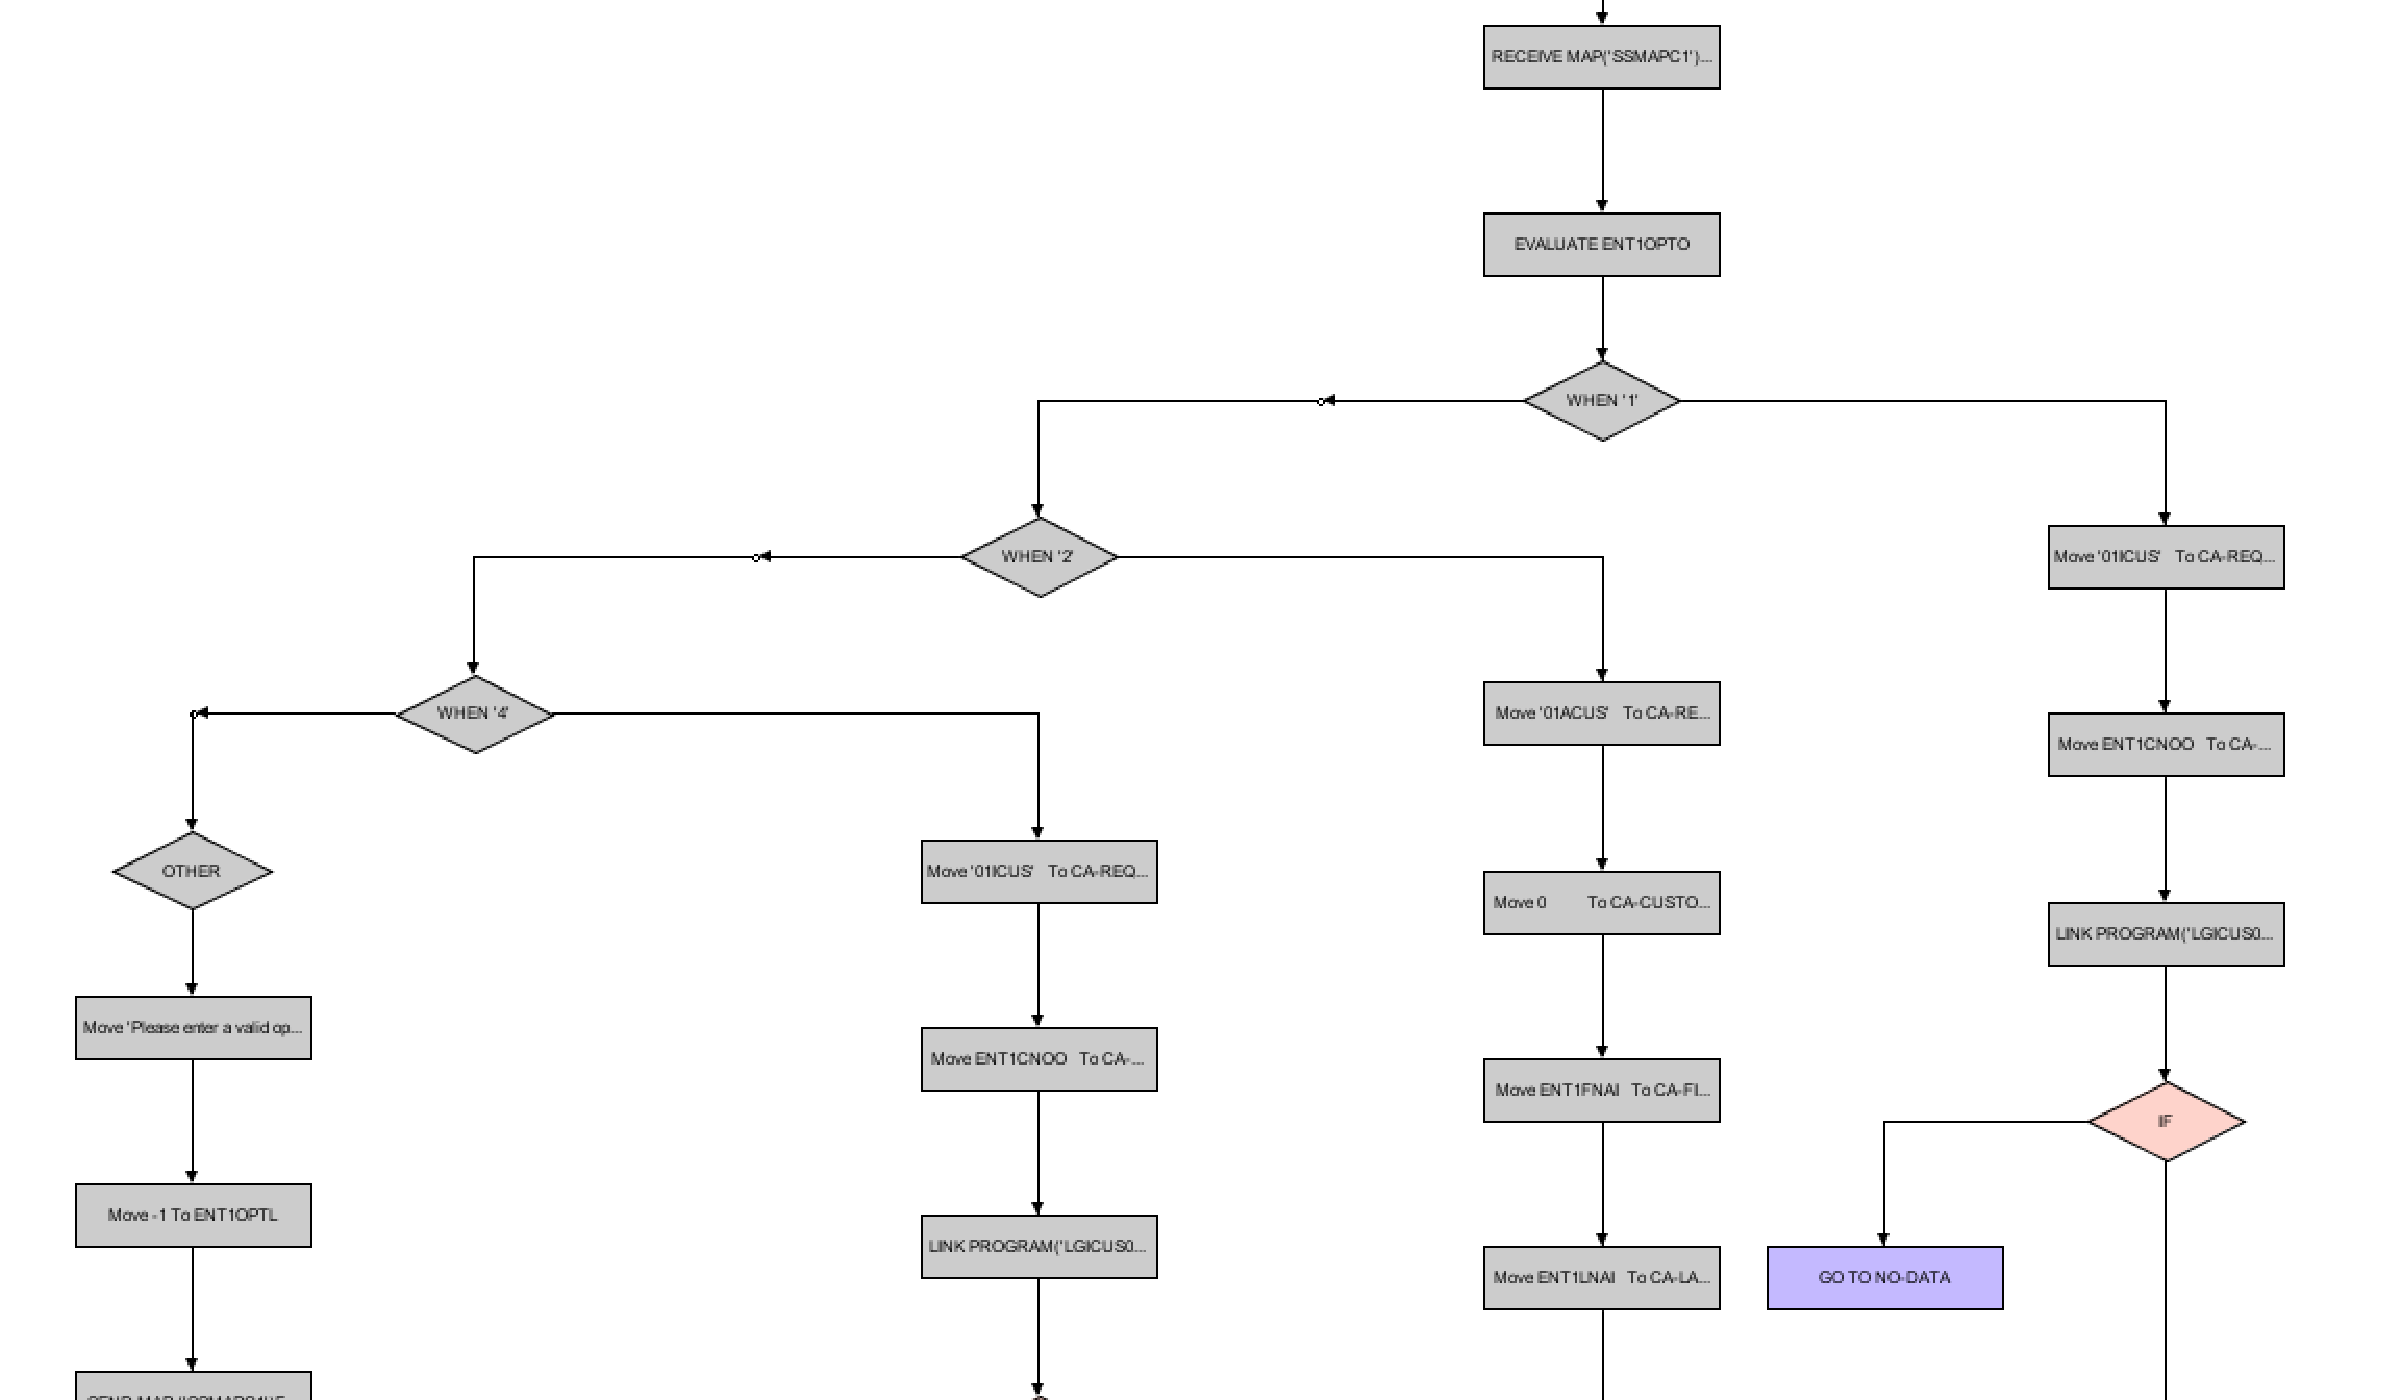
\includegraphics[scale=0.35]{images/kapitel_4/ibmad_flowchartSwitch.pdf}
  \caption{Die Switch-Verzweigung der GenApp}
  \label{fig:ibmad_flowchartSwitch}
\end{figure}

Das Flow-Diagram lässt sich in IBM Application Discovery mit der Schaltfläche \path{Flow Chart} anzeigen und es wird ein
Diagramm wie in Abbildung \ref{fig:ibmad_graph} auf Seite \pageref{fig:ibmad_graph} sichtbar.

In diese kann dann nach belieben rein- und rausgezoomt werden. Auch lassen sich Bilder extrahieren und Programmteile
genauer untersuchen.

\begin{figure}[h]
  \centering
    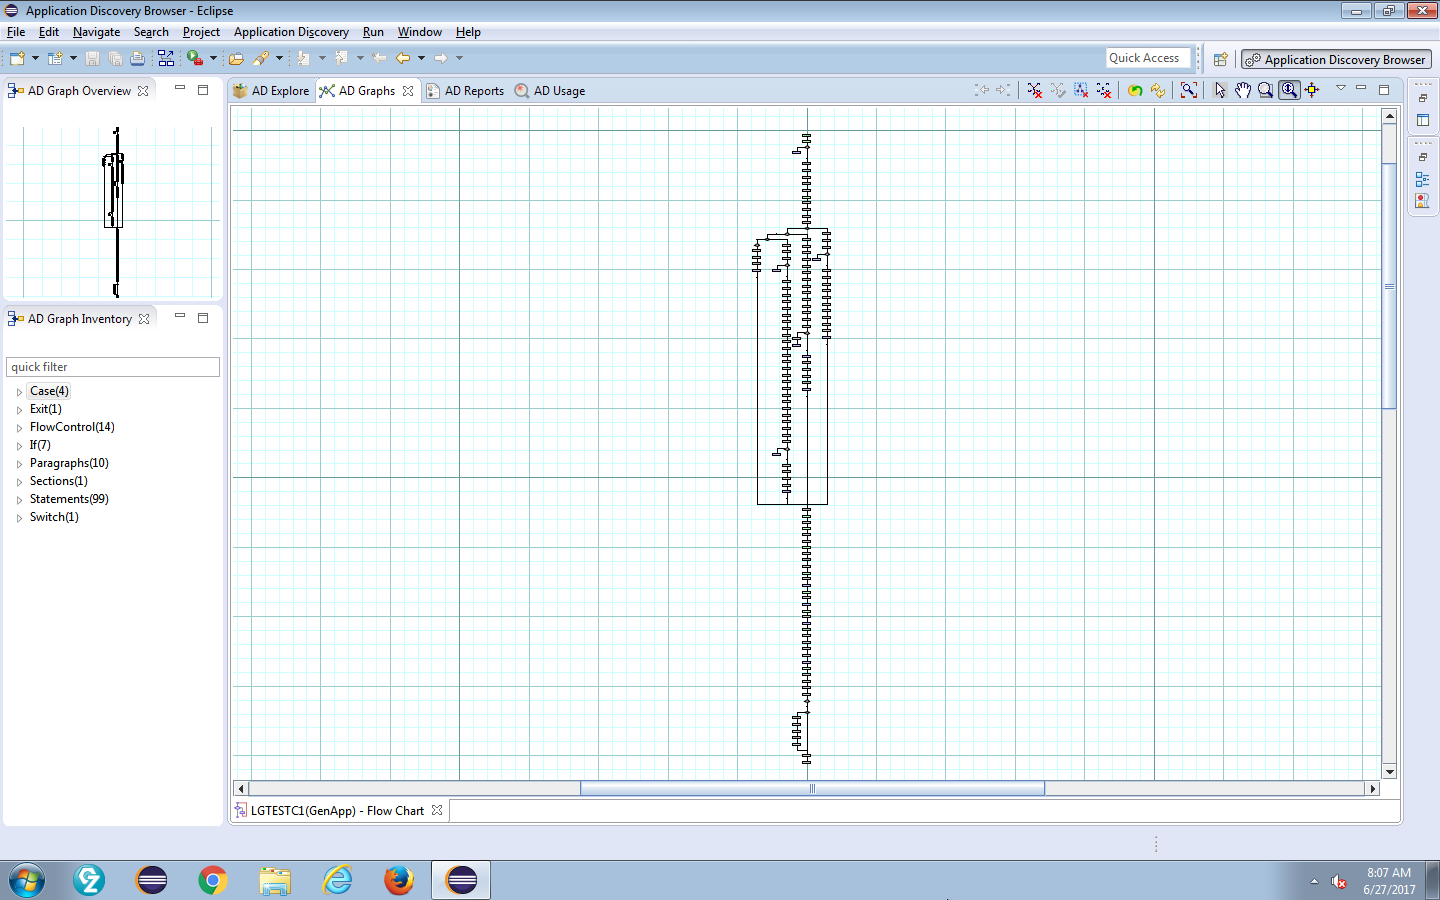
\includegraphics[scale=0.28]{images/kapitel_4/ibmad_graph.png}
  \caption{Anzeigen des Flow Charts}
  \label{fig:ibmad_graph}
\end{figure}

Aus dem Flow-Chart und der daraus extrahierten Switch-Verzweigung lässt sich eine wichtige Kenntnis ableiten. Das
Hauptprogramm startet je nach Auswahl des Benutzers eine von drei unterschiedlichen Programmen. Diese Information kann
nun für die Definition der Schnittstellen genutzt werden.

\subsubsection{Definieren der Schnittstellen}
Da die Anwendung nun analysiert ist, können die verwendeten Schnittstellen der Anwendung ausgewählt und dokumentiert
werden. Bei den Schnittstellen handelt es sich lediglich um die einzelnen Aufrufe, welche bei der Switch-Verzweigung
in LGTESTC1 aufgerufen werden. Siehe dazu \ref{fig:ibmad_flowchartSwitch} auf Seite \pageref{fig:ibmad_flowchartSwitch}.

Damit der Java-Wrapper mit der COBOL-Anwendung genutzt werden kann muss dieser die Programmteile \path{LGICUS01},
\path{LGACUS01} und \path{LGUCUS01} starten können. Diese sind für die Verarbeitung der Daten zuständig.

Dabei ist \path{LGACUS01} für das Hinzufügen eines neuen Customers zuständig. Der Java-Wrapper muss dem Programm die
Informationen wie \textit{Vorname}, \textit{Nachname}, \textit{Wohnort}, \textit{Straßenname} und \textit{Telefonnummer}
übergeben.

Das Teilprogramm \path{LGUCUS01} kann einen Eintrag eines Customers aktualisieren. Dazu werden die neuen Werte als
Parameter übergeben. Dabei handelt es sich um die Selben wie bei LGACUS01.

Im letzten Programm, \path{LGICUS01}, werden Informationen des Customers zurückgegeben. Dazu werden keine Parameter zum
Aufruf benötigt. Lediglich werden Daten zurück an den Java-Wrapper gegeben.

Die Kommunikation zwischen Java-Wrapper und COBOL-Anwendung wird mittels der WOLA-Schnittstelle gewährleistet.

Diese Informationen können dazu genutzt werden, um den Java-Wrapper zu bauen, damit die COBOL-Anwendung für die Cloud
bereitgestellt werden kann.

\subsection{CICS Region erstellen}
Da nun die COBOL-Anwendung analysiert ist, kann eine CICS-Region erstellt werden, welche sowohl die COBOL-Anwendung
als auch den späteren Java-Wrapper beinhalten wird.

Dazu wird der instanziierte \path{Service Broker zOSMF} geöffnet und dann der Tab \path{CICS} ausgewählt. Nun werden alle
schon eingerichteten CICS-Regionen angezeigt.

Um eine neue Region zu erstellen, wird auf den Button \path{ADD CICS} geklickt, worauf sich ein Fenster öffnet, in dem
Informationen eingegeben werden müssen. Siehe dazu Abbildung \ref{fig:image_cicsErstellen} auf Seite
\pageref{fig:image_cicsErstellen}.

\begin{figure}[h]
  \centering
    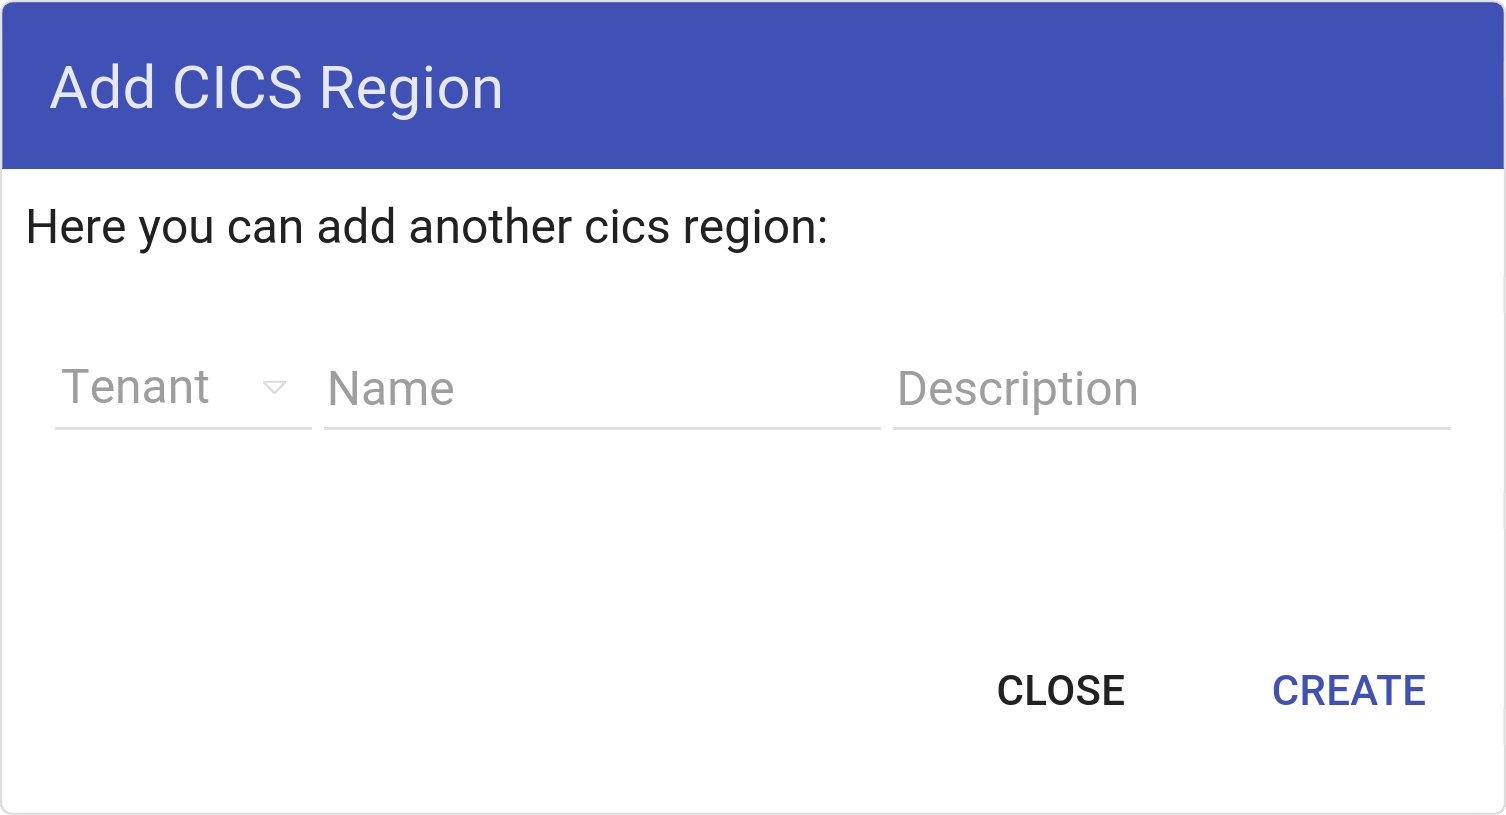
\includegraphics[scale=0.2]{images/kapitel_4/image_cicsErstellen.png}
  \caption{Erstellen einer CICS Region}
  \label{fig:image_cicsErstellen}
\end{figure}

Nach der Auswahl eines Tenanten (Standort), der Eingabe eines Namens und einer Beschreibung kann auf \path{CREATE} geklickt
werden, worauf die neue CICS-Region eingerichtet wird. Dieser Vorgang dauert ein paar Sekunden.

Im Anschluss wird die neue CICS-Region in der Übersicht angezeigt. Sie kann nun ausgewählt werden, um weitere Informationen
anzuzeigen. Insbesondere die Information über den \path{Port} spielt für die weitere Vorgehensweise eine wichtige Rolle.

\subsection{Verbindung aufbauen}
Da nun eine neue CICS-Region erstellt wurde, muss im Secure Gateway Service in Bluemix ein Eintrag für diese hinzugefügt
werden. Dies ermöglicht die Kommunikation mit der Region via URL und Port.

Dazu wird der Secure Gateway Service in Bluemix geöffnet und der eingerichtete Client angeklickt. Damit öffnet sich die
Übersicht über alle registrierten \path{Ziele}.

Über den großen grünen Knopf kann ein neues Ziel hinzugefügt werden. Dabei wird zuallererst nach dem Standort des Ziels
gefragt. Da sich die CICS-Region auf dem Mainframe befindet, wird hier \path{Lokal} ausgewählt.

Mit einem Klick auf \path{Weiter} wird nach dem Hostname und dem Port gefragt. Der Hostname ist die IP-Adresse des z/OS-Systems
(hier im Beispiel die \path{10.3.20.47}) und der Port ist der der neu erstellten CICS-Region. Hier im Beispiel also die
\path{54300}. Im Anschluss kann auf \path{Weiter} geklicken werden.

Nun können Zertifikate für die Autorisierung hochgeladen und die Art des Protokolls definiert werden. Hier im Beispiel
werden keine Zertifikate genutzt, und das Protokoll ist \path{TCP}, da dieses Protokoll auch für die Kommunikation zwischen
Ubuntu- und z/OS-System genutzt wird. Mit einem Klick auf \path{Weiter} wird dies bestätigt.

Im Folgenden kann die Authentifizierung ausgewählt werden. Da nun erstmal keine genutzt wird, kann die Auswahl bei
\path{None} gelassen und mittels \path{Weiter} gespeichert werden.

Da die Verbindung nicht eingeschränkt werden soll, kann das nächste Fenster einfach mit \path{Weiter} gespeichert werden,
worauf die Eingabe eines Namens für das Ziel folgt.

In diesem wird als Name \path{REST-Interface} genutzt, da in dieser CICS-Region sowohl die COBOL-Anwendung als auch das
REST-Interface laufen wird. Nach der Eingabe kann das Ziel gespeichert werden und es wird direkt in der Übersicht angezeigt.

Mit einem Klick auf das Zahnrad des jeweiligen Ziels öffnet sich ein Fenster mit verschiedenen Informationen zu diesem.
Dabei ist der Eintrag \path{Cloud-Host: Port} wichtig, da dieser die URL für die CICS-Region anzeigt, die im Web-Frontend
genutzt wird um die REST-Schnittstelle anzusprechen.

\subsection{Toolchain konfigurieren}
In Kapitel \ref{subsec:einrichten_der_toolchain} auf Seite \pageref{subsec:einrichten_der_toolchain} wurde die Toolchain
zum Bauen des Artefaktes aus dem Quellcode schon grundsätzlich eingerichtet. Da nun eine CICS-Region für das Backend
eingerichtet wurde und die Verbindung zwischen Bluemix und CICS-Region auf dem Mainframe hergestellt wird, kann nun auch
der Buildprozess darauf angepasst werden.

Dazu wird die Toolchain in Bluemix geöffnet und im Dashbaord dann die Build Pipeline ausgewählt. In dieser sind zwei Stages
vorkonfiguriert. Die \path{BUILD}-Stage baut immer nach einem \textit{push} in das Git-Repository ein Artefakt aus dem
Quelltext. Dieses Artefakt gibt sie weiter an die \path{DEPLOY}-Stage. Diese kann das Artefakt auf einem System
installieren. In diesem Fall muss diese angepasst werden.

Über das Zahnrad-Symbol am rechten oberen Rand der \path{BUILD}-Stage wird die Konfiguration geöffnet. In dem sich
öffnenden Fenster wird unter \path{Jobs} über den Button \path{Job hinzufuegen} ein neuer hinzugefügt. Der Typ dabei ist
\path{Build}. Dieser erhält als Namen zum Beispiel \path{Deploy on CICS}. Als Buildtyp wird \path{Shell-Script} ausgewählt
und das Build-Script kann in Listing \ref{Build-Script für CICS-Region} auf Seite \pageref{Build-Script für CICS-Region}
eingesehen werden.

\begin{lstlisting}[language=bash, caption=Build-Script für CICS-Region, label=Build-Script für CICS-Region]
    #!/bin/bash
    sudo apt-get update && sudo apt-get install lftp
    lftp -u username,password -e 'mirror ./GenAppService.war /var/cicsts/CICSF000/workdir/DFHWLP/wlp/usr/servers/defaultServer/dropins/' secureGatewayURL:PORT
\end{lstlisting}

Dabei sind die Parameter \path{username} und \path{password} die, eines Benutzers auf der z/OS Maschine. Dabei können es
die Selben der zOSMF-Schnittstelle sein. Der Benutzer muss lediglich Schreibrechte im \path{dropins}-Verzeichnis haben.

Der Parameter \path{secureGatewayURL} mit zugehörigem \path{PORT} ist in Bluemix im Secure Gateway Service zu finden,
nachdem die CICS-Region damit verbunden wurde.

Durch dieses Shell-Script, wird in einer Virtuellen Umgebung in der Toolchain das Programm
\path{LFTP}\footnote{https://lftp.yar.ru} installiert. Anschließend wird mit Hilfe des Programms das Artefakt aus dem
vorhergehenden Build-Step auf die CICS-Region kopiert und gegebenenfalls überschrieben.

Da die CICS-Region einen WebSphere Liberty Server enthält und dieser Application Server alle \path{.war}-Files im
\path{dropins}-Verzeichnis automatisch einbindet, kann die \path{GenAppService.war}-Datei einfach dort abgelegt werden.
Nach wenigen Sekunden importiert der Server die Datei dann automatisch und stellt sie dem Benutzer zur Verfügung.

Nun wird nach jedem \textit{push} in das Git-Repository automatisch der Build and Deploy vorgang (Build Pipeline) gestartet
und die neueste Version der Anwendung auf der verbundenen CICS-Region installiert.

\subsection{Runtime hinzufügen}
\label{subsec:runtime_hinzufügen}
Da nun die Verbindung zwischen Cloud-Infrastruktur und CICS-Region hergestellt ist, kann im nächsten Schritt die Runtime
für das Web-Frontend instanziiert und eingerichtet werden.

Um in Bluemix eine Runtime für NodeJS-Applikationen zur Verfügung zu stellen, gibt es zwei Möglichkeiten.

\subsubsection{Einrichtung mittels Bluemix Dashbaord}
\label{subsubsection:bluemixDashbaord}
Die Einrichtung einer Runtime für NodeJS mittels Bluemix Dashboard startet mit einem Aufruf des \path{Katalogs} in Bluemix.
In diesem gibt es unter der Kategorie \path{Apps} und \path{Cloud Foundry-Anwendungen} den Eintrag \path{SDK for NodeJS}.

Ein Klick auf den Eintrag öffnet die Übersicht des Services. Der Name definiert den Namen der Runtime wie sie unter
Bluemix aufgelistet wird. Der Hostname definiert die URL, über die die Anwendung aufrufbar ist. Sie folgt dabei dem Schema
\path{https://hostname.mybluemix.net}.

Nach dem Klick auf \path{Erstellen} wird die Runtime eingerichtet und vorbereitet. Dieser Schritt dauert je nach
Gesamtauslastung von Bluemix wenige Sekunden.

Im Anschluss ist die Runtime im Dashboard von Bluemix zu finden und einsatzbereit. Der Aufruf der definierten Domain
im Webbrowser öffnet eine Standardseite mit Informationen zur Runtime.

\subsubsection{Einrichtung mittels Cloud Foundry CLI}
Eine Alternative zur Einrichtung der Runtime via Dashboard ist die Einrichtung via Cloud Foundry CLI. Dazu wird die CF CLI
mittels \path{login} mit der aktuellen Organisation und dem Bereich verbunden und im Anschluss mittels \path{create-service}
eine SDK for NodeJS eingerichtet.

\begin{lstlisting}[language=bash, caption=Provisionieren des SDK for NodeJS Services, label=Provisionieren des SDK for NodeJS Services]
   $ cf create-service sdk_for_nodejs standard appName
\end{lstlisting}

Dabei ist \path{sdk_for_nodejs} der Name des Service, der instanziiert werden soll. Der Parameter \path{standard} gibt an,
dass der einzig verfügbare Plan genutzt werden soll. Als letztes gibt \path{appName} den Hostnamen, welcher verwendet
werden soll, an.

Die Einrichtung sollte innerhalb weniger Sekunden abgeschlossen sein, und die Runtime wird im Bluemix Dashboard angezeigt.
Alle aktiven Runtimes mit Name und Hostname können über den Befehl \path{apps} aufgelistet werden.

\begin{lstlisting}[language=bash, caption=Auflisten aller Applikationen, label=Auflisten aller Applikationen]
   $ cf apps
\end{lstlisting}

Nun kann die Anwendung über den definierten \path{appName} in einem Webbrowser aufgerufen werden, und es erscheint eine
Standartseite mit Informationen zur Runtime.

\subsection{Text2Speech-Service hinzufügen}
Da nun die Runtime für das Web-Frontend erstellt und eingerichtet ist, kann der zusätzlich genutzte Service \path{Text2Speech}
instanziiert werden. Dieser wandelt geschriebenen Text in eine Audio-Datei um, die von modernen Webbrowsern abgespielt
werden kann.

Da dies, genau wie die Runtime SKD for NodeJS, auch ein Service ist, gibt es auch hier beide Möglichkeiten der Einrichtung,
entweder über das Bluemix Dashboard oder über das Cloud Foundry CLI. Der einfachheithalber wird hier nur der Weg mittels
CLI aufgezeigt. Die Einrichtung mittels Bluemix Dashboard erfolgt analog zu Kapitel \ref{subsubsection:bluemixDashbaord}
auf Seite \pageref{subsubsection:bluemixDashbaord}.

Mit \path{create-service} wird der Service dem Bluemix Account hinzugefügt und steht ab dann zur Verfügung.

\begin{lstlisting}[language=bash, caption=Provisionieren des Text2Speech Services, label=Provisionieren des Text2Speech Services]
   $ cf create-service text_to_speech standard serviceName
\end{lstlisting}

Mit dem Befehl \path{services} können alle instanziierten Services in der Organisation und dem Bereich angezeigt werden.

\begin{lstlisting}[language=bash, caption=Auflisten aller instanziieren Services, label=Auflisten aller instantiieren Services]
   $ cf services
\end{lstlisting}

\subsection{Runtime verbinden}
Damit die SDK for NodeJS Runtime und der Service Text2Speech über die \path{VCAP} Variablen kommunizieren können, müssen
die App und der Service verbunden werden. Um diesen Schritt durchzuführen, gibt es zwei Möglichkeiten.

\subsubsection{Binden über Bluemix Dashboard}
Um die Runtime und den Service über das Bluemix Dasboard zu verbinden, muss die Übersichtsseite der SDK for NodeJS Runtime
geöffnet werden. Auf dieser Übersichtsseite gibt es den Tab \path{Verbindungen}. In diesem werde alle Verbindungen zwischen
Runtime und Services angezeigt. Zur Zeit existieren noch keine.

Mit einem Klick auf \path{Vorhandenen verbinden} kann der schon erstellte Text2Speech Service verbunden werden. In der sich
öffnenden Seite wird dieser dazu einfach ausgewählt und mittels \path{Verbindung herstellen} gespeichert.

Die Frage, ob die Runtime neu gestaged (neugestartet und verbunden) werden darf, muss mit \textbf{Ja} bestätigt werden.
Die Runtime steht ab dann für wenige Sekunden nicht zu Verfügung.

Anschließend erscheint der Text2Speech Service auf der Übersichtsseite der Runtime im Tab \path{Verbindungen}.

\subsubsection{Binden über Cloud Foundry CLI}
Alternativ kann die Verbindung über die Cloud Foundry CLI durchgeführt werden. Dazu wird die Funktion \path{bind-service}
nach einem vorangegangenen \path{login} genutzt.

\begin{lstlisting}[language=bash, caption=Binden der Runtime mit dem Service, label=Binden der Runtime mit dem Service]
   $ cf bind-service appName serviceName
\end{lstlisting}

Dabei wird als \path{appName} der vergebene Name der NodeJS-Runtime angegeben. Als \path{serviceName} der Name, der an den
Text2Speech Service vergeben wurde.

Anschließend muss die Runtime mittels \path{restart} neugestartet werden.

\begin{lstlisting}[language=bash, caption=Neustarten der Runtime, label=Neustarten der Runtime]
   $ cf restart appName
\end{lstlisting}

Dabei wird wieder als \path{appName} der Name der NodeJS-Runtime angegeben.

Die erfolgreiche Verbindung der Runtime und des Service ist in der Übersichtsseite der Runtime im Bluemix Dashboard im
Tab \path{Verbindungen} sichtbar.

\subsection{Erstellen des Backends}
Damit das Frontend die Daten aus der Datenbank visualisieren kann, müssen diese aus dem Backend abgerufen werden. Dies kann
auf zwei Arten geschehen.

In der ersten Möglichkeit ruft das Frontend die Daten durch den Java-Wrapper ab, der wiederum die Daten durch die
COBOL-Anwendung von der Datenbank erhält.

Alternativ kann das Frontend auch einen REST-Service der DB2 abrufen, welcher aufgrund eines hinterlegten SQL-Befehls
Daten zurückgeben kann.

Ein Auszug des Datenbankaufbaus ist in Anhang \ref{anhang:datenbankschema} auf Seite \pageref{anhang:datenbankschema}
zu sehen. Da die GenApp schon verschiedene Daten aus der Datenbank zurückgeben kann, wird der DB2 Service nur für die
Daten genutzt, welche nicht durch die GenApp erfasst werden. Somit können beide Varianten nebeneinander koexistieren, ohne
sich zu überlagern.

Ein weiterer Grund ist, dass die COBOL-Anwendung in ihrer Funktionalität nicht erweitert werden soll.

\subsubsection{DB2 REST Services}
Da die COBOL-Anwendung lediglich die \textit{Kundeninformationen} und die \textit{Policies} aus der Datenbank lesen kann,
und keine Information darüber hat, welcher Kunde welche Policy besitzt, wird ein DB2 Rest Service eingerichtet, der diese
Information auflösen kann.

Um einen DB2 REST Service anzulegen, wird ein Package in der DB2 Instanz eingerichtet. Dieses Package enthält eine
SQL-Abfrage und wird im \path{SYSIBM.DSNSERVICE} Katalog abgelegt.

Ein authentifizierter Benutzer kann sich alle für ihn sichtbaren Services anschauen, diese ausführen und einen neuen
einrichten.

Weitere Informationen über den Service sind im IBM Knowledge
Center\footnote{https://www.ibm.com/support/knowledgecenter/SSEPEK\_11.0.0/restserv/src/tpc\\/db2z\_restservices.html} zu
finden.

Da es sich bei der prototypischen Anwendung um eine Web-Anwendung handelt, welche direkt mit dem DB2 REST Service
kommunizieren wird, muss die DB2 Instanz CORS zulassen.

Dazu wird im z/OS-System, in welchem die DB2 Instanz läuft, in der Datei \path{/qibm/userdata/qwebqry/WQLIB85/conf/httpd.conf}
der Header für CORS - \\ \path{Access-Control-Allow-Origin} - gesetzt.

Für die Bearbeitung der Datei wird diese zum Beispiel mit \path{nano} geöffnet.

\begin{lstlisting}[language=bash, caption=Bearbeiten der Konfigurationsdatei, label=Bearbeiten der Konfigurationsdatei]
   $ nano /qibm/userdata/qwebqry/WQLIB85/conf/httpd.conf
\end{lstlisting}

Im Anschluss wird im \path{Location}-Tag der Header-Wert hinzugefügt.

\begin{lstlisting}[caption=Header für CORS setzen, label=Header für CORS setzen]
   $ Header set Access-Control-Allow-Origin "*"
\end{lstlisting}

Da nun mittels JavaScript-Requests der REST Service aufgerufen werden kann, kann dieser eingerichtet werden. Dazu wird
ein \path{POST}-Request an den DB2ServiceManager geschickt, welcher die Informationen für den Service beinhaltet.

Zum Ausführen des \path{POST}-Requests wird \path{Postman} genutzt. Dabei wird als URL die des DB2ServiceManager angegeben.

\begin{lstlisting}[language=bash, caption=DB2 REST Service erstellen, label=DB2 REST Service erstellen]
   POST https://<host>:<port>/services/DB2ServiceManager
\end{lstlisting}

Als \path{POST}-Parameter werden neben Typ und Name auch der SQL-Befehl übergeben, welcher ausgeführt werden soll, wenn der
Service aufgerufen wird.

\begin{lstlisting}[language=json, caption=Parameter zur Erstellung, label=Parameter zur Erstellung]
    {
        "requestType":  "createService",
        "sqlStmt":      "<sqlStatement>",
        "collectionID": "<serviceCollectionID>",
        "serviceName":  "<serviceName>",
        "description":  "<serviceDescription>"
    }
\end{lstlisting}

Dabei ist \path{requestType} der Typ der Anfrage. Dieser muss \path{createService} sein, da ein neuer Service in der
DB2 Instanz eingerichtet werden soll.

Bei \path{sqlStmt} handelt es sich um das SQL-Statement, welches bei einem Aufruf des Services ausgeführt werden soll.
Dabei gelten die Rechte des Nutzers, mit welchem der REST Service eingerichtet wurde.

Die \path{collectionID} ist der Benutzername für welchen der Service eingerichtet werden soll.

Der \path{serviceName} kann frei vergeben werden. Er wird beim Aufruf des Services genutzt, um ihn eindeutig zu
identifizieren und anzusprechen. In diesem Beispiel wird dafür \path{getPolicyByCustomer} genutzt.

Im Parameter \path{description} kann noch eine optinale Beschreibung des Services hinzugefügt werden.

Der Aufruf muss als eingeloggter Benutzer erfolgen. Dazu wird in Postman im Bereich \path{Authorization} der Type
\path{Basic Auth} ausgewählt und in die beiden Felder der Benutzername und das zugehörige Passwort eingetragen, für den
der Service eingerichtet werden soll. Der Benutzername muss der Selbe sein, welcher im POST-Parameter \path{collectionID}
verwendet wird.

Die Antwort des Servers nach dem Ausführen des Requests bestätigt die erfolgreiche Einrichtung des Services und zeigt die
\path{URL} an, welche zur Nutzung des Services genutzt wird.

\begin{lstlisting}[language=json, caption=Antwort des Servers, label=Antwort des Servers]
    {
     "StatusCode": 201,
     "StatusDescription": "DB2 Rest Service getPolicyByCustomer was created successfully.",
     "URL": "http://<host>:<port>/services/SYSIBMSERVICE/getPolicyByCustomer"
    }
\end{lstlisting}

Der HTTP-Statuscode mit \path{201} gibt an, dass der Service erfolgreich erstellt wurde.

Für die Anwendung ist die getPoliciesByCustomer-URL, \path{http://<host>:<port>/services/SUCI101/getPoliciesByCustomer},
erfolgreich eingerichtet worden.

\subsubsection{Secure Gateway Ziel}
Damit das Web-Frontend auf den erfolgreich eingerichteten DB2 REST Service zugreifen kann, um die Daten aus der Datenbank
auszulesen, muss nun ein weiteres Ziel für den Secure Gateway hinzugefügt werden.

Dies geschieht wie in Kapitel \ref{subsection:secureGateway} auf Seite \pageref{subsection:secureGateway} beschrieben.
Dabei ist der Name des Ziels nun \path{DB2 REST Service}. Die IP-Adresse und der Port sind die, welche nach erfolgreicher
Ausführung des \path{POST}-Request an den DB2ServiceManager zurückgegeben wurden. Siehe dazu Listing
\ref{Antwort des Servers} auf Seite \pageref{Antwort des Servers}.

\subsubsection{Java-Wrapper}
Damit das Web-Frontend Informationen aus der Datenbank über die schon analysierte COBOL-Anwendung abrufen kann, muss diese
mit einer Schnittstelle versehen werden. Diese Schnittstelle wird in Form eines Java REST-Interfaces zur Verfügung
gestellt, welches die Kommunikation zwischen Web-Frontend und COBOL-Anwendung übernimmt.

Damit der Java-Wrapper aus der Cloud über den Secure Gateway aufgerufen werden kann, muss der Application Server CORS
akzeptieren. Um CORS in WebSphere Liberty zu aktivieren muss der Header in der Konfiguration gesetzt werden.

Dazu wird in der jeweiligen \path{server.xml}-Datei im WebSphere-Verzeichnis der CICS-Anwendung der \path{cors}-Tag
eingefügt. Siehe dazu Listing \ref{Konfiguration von CORS} auf Seite \pageref{Konfiguration von CORS}.

\begin{lstlisting}[language=html, caption=Konfiguration von CORS, label=Konfiguration von CORS]
    <cors domain="*"
          allowedOrigins="*"
          allowedMethods="GET, DELETE, POST, OPTION"
          allowedHeaders="accept"
          allowCredentials="true"
          maxAge="3600" />
\end{lstlisting}

Durch diese Konfiguration kann jeder Client, symbolisiert durch \path{allowedOrigins="*"}, auf alle Entpunkte des
REST-Interfaces, \path{domain="*"}, zugreifen und das Interface nutzen.

Im Normalfall würde CORS bei \path{allowedOrigins="*"} nicht mit einem * konfiguriert werden, sondern
auf die wenigen Clients eingeschränkt, die wirklich Zugriff brauchen. Da bei der Entwicklung allerdings von
verschiedenen Testsystemen und produktiven Hosts zugegriffen wird, wird der Zugriff für die Entwicklungsdauer nicht
eingeschränkt.

Da nun CORS vom Server akzeptiert wird, kann das eigentliche Interface entwickelt werden. In Abbilung
\ref{fig:swagger_genappbackend} auf Seite \pageref{fig:swagger_genappbackend} ist das Interface definiert, was der
Java-Wrapper bereitstellen muss.

\begin{figure}[h]
  \centering
    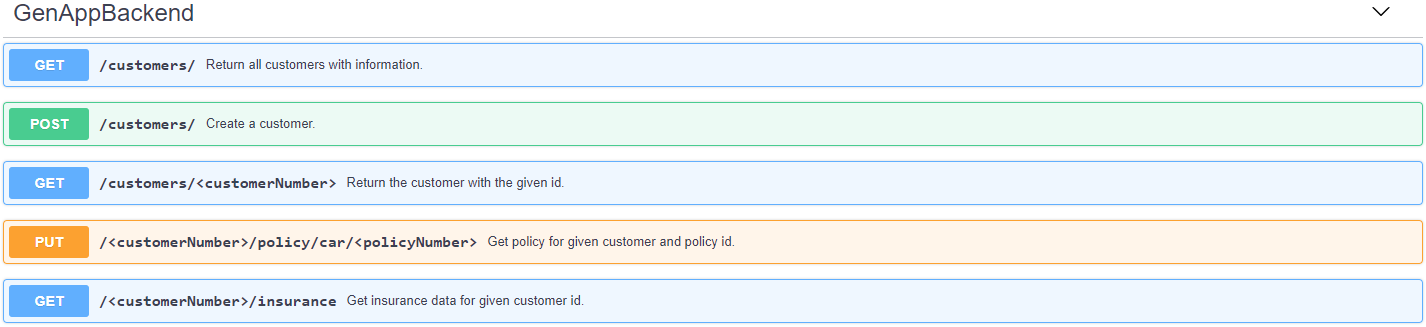
\includegraphics[scale=0.38]{images/kapitel_4/swagger_genappbackend.png}
  \caption{Übersicht des Backend-Interface}
  \label{fig:swagger_genappbackend}
\end{figure}

Für die Entwicklung des REST-Interfaces wird \path{Jersey}\footnote{https://github.com/jersey/jersey} genutzt. Mit Jersey
lässt sich ein Servlet-Endpunkt definieren, sodass der RESTful Web-Service in einem Servlet-Container wie dem WebSphere
Liberty läuft.

Bei Jersey werden über einzelne Funktionen \textit{Annotations} geschrieben, welche die zentrale Konfiguration des
Interfaces vornehmen. In Listing \ref{Beispiel eines REST-Endpunktes} auf Seite \pageref{Beispiel eines REST-Endpunktes}
ist eine Beispielimplementierung eines REST-Endpunktes zu sehen.

\begin{lstlisting}[language=java, caption=Beispiel eines REST-Endpunktes, label=Beispiel eines REST-Endpunktes]
    package de.larsprobst.rest;

    import javax.ws.rs.*;

    @Path("sayHello")
    public class MessageResource
    {
        @GET
        @Produces(MediaType.TEXT_PLAIN)
        public String message()
        {
            return "Hello";
        }
    }
\end{lstlisting}

In diesem kleinen Beispiel wird ein Endpunkt mit \path{/sayHello} erstellt, welcher über den Aufruf mit der HTTP-Methode
\path{GET} den Text \textit{Hello} zurück liefert.

In dieser Art werden alle benötigten Endpunkte für das REST-Interface definiert und mit Hilfe von Klassen werden
Objekte für Kundendaten und Policies erstellt.

Außerdem wird in einem Package die WOLA-Verbindung zur COBOL-Anwendung aufgebaut. Dies geschieht in diesem Beispiel über
die Klasse \path{GenAppJCAImpl.java}, welche alle Programmteile der COBOL-Anwendung kennt und diese nach Bedarf mit den
benötigten Parametern aufrufen kann.

Über die Klasse \path{GenAppCommarea.java} wird die Kommunikation zwischen Java- und COBOL-Anwendung definiert. Dort werden
die Java-Variablen auf die COBOL-Datentypen gemappt. Dies geschieht wie in Listing \ref{Java-Variable auf COBOL-Datentyp mappen}
auf Seite \pageref{Java-Variable auf COBOL-Datentyp mappen} beschrieben.

\begin{lstlisting}[language=java, caption=Java-Variable auf COBOL-Datentyp mappen, label=Java-Variable auf COBOL-Datentyp mappen]
    protected static final StringField CA_LAST_NAME = factory.getStringField(20);
\end{lstlisting}

In diesem Beispiel wird die Java-Variable \path{CA_LAST_NAME} auf einen COBOL-Datentyp gemappt, welcher insgesamt 20 Zeichen
besitzt. Die \path{factory} ist dabei vom Typ \path{CobolDatatypeFactory}, welche automatisch mit
\path{Java Batch Toolkit for z/OS (JZOS)} erstellt werden kann. Dabei analysiert das IBM Tool die genutzte COBOL-Anwendung
und erstellt die Klasse automatisiert.

Der Quelltext des Java-Wrappers ist im zugehörigen GitHub-Repository\footnote{https://github.com/Alienuser/GenAppBackend}
zu finden und kann dort heruntergeladen und genutzt werden.

\subsection{Erstellen des Web-Frontends}
Da nun die Schnittstellen des Java-Wrappers und auch die Rückgabewerte der Datenbank bekannt sind, kann das Web-Frontend
entwickelt werden. Dafür werden zuerst Use-Cases gesammelt, welche auf dem Frontend umgesetzt werden sollen. Anschließend
wird ein Mockup erstellt, welches das Design und die Anordnung darstellt.

Mit dem Web-Frontend soll es möglich sein, einerseits Daten aus der Datenbank über die COBOL-Anwendung mit Java-Wrapper
zu laden, als auch über den DB2 REST Service.

Außerdem soll ein weiterer Bereich entstehen, in dem Daten aus einem Watson-Service gelesen werden können. Dabei handelt
es sich um einen Kundenwert des Nutzers, welcher anhand von Beispieldaten berechnet wird.

Die Daten sollen nicht nur einmalig aus der Datenbank geholt werden, sondern via \textit{polling} alle 15 Sekunden. Die
Idee dahinter ist, dass Daten in der Datenbank abgeändert werden können und sich diese nach maximal 14 Sekunden auch im
Frontend ändern. Da CICS-Regionen zur Zeit kein \textit{Web-Socket} unterstützen, muss dies via \textit{polling} gelöst
werden.

Da das Frontend auch in den Smartphone-Apps angezeigt werden soll ist es wichtig, dass es sich der Größe des Bildschirmes
anpasst, mit dem es angezeigt wird. Allgemein ist es wichtig, eine Mobile-First- oder Responsive-Webseite zu erstellen.

Das entstandene Mockup kann in Abbildung \ref{fig:mockup_website} auf Seite \pageref{fig:mockup_website} angesehen werden.
Dabei fällt auf, dass es neben den Boxen für die Informationen auch eine Navigationsleiste mit zwei Menüpunkten gibt.

\begin{figure}[h]
 \centering
   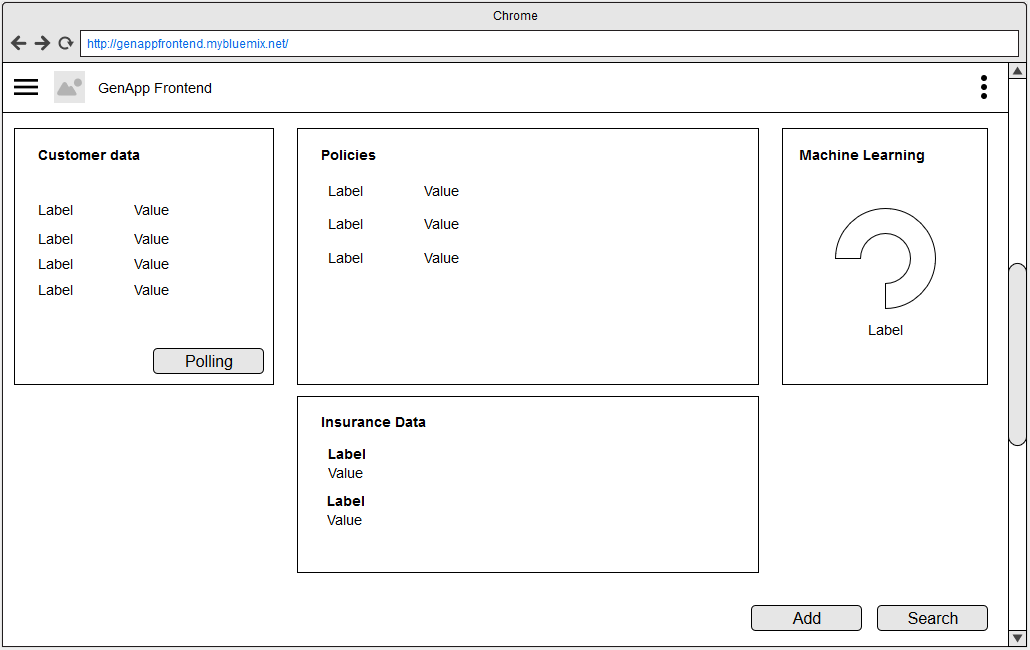
\includegraphics[scale=0.5]{images/kapitel_4/mockup_website.png}
 \caption{Mockup des Web-Frontends}
 \label{fig:mockup_website}
\end{figure}

Der linke Menüpunkt (auch \textit{Burgermenü} genannt), öffnet das seitliche Navigationsmenü. Dort gibt es allerdings nur einen
Eintrag, welcher auch standardmäßig geöffnet und ausgewählt ist. Die Idee dabei ist, dass das Frontend in Zukunft
weiterentwickelt werden kann und dann mehrere Menüpunkte benötigt werden, welche alle in diesem seitlichen Menü angezeigt
werden können.

Das rechte Menü mit den drei übereinanderstehenden Punkten symbolisiert ein Kontextmenü, welches ein Dropdown öffnet. In
diesem gibt es zwei Menüeinträge. Einen \path{Settings} und einen \path{Info} Eintrag. Ersterer kann die verwendete URL
des Secure Gateways überschreiben, damit für Demonstrationszwecke andere Endpunkte genutzt werden können.

Zweiterer öffnet ein modales Fenster, welches Informationen über die vorliegende App
anzeigt, einen Link zum GitHub-Repository beinhaltet und Kontaktmöglichkeiten mit dem Autoren zur Verfügung stellt.

Am unteren rechten Bildschirmrand wird es zwei Buttons geben. Einer wird eine Suche nach einer Kundennummer ermöglichen.
Der Andere öffnet ein modales Fenster, mit welchem ein neuer Benutzer in die Datenbank eingetragen werden kann.

Nach jeder Suche oder der Anzeige von Daten soll am unteren linken Bildschirmrand eine kleine Informationsbox erscheinen,
welche Informationen anzeigt. So zum Beispiel das erfolgreiche Auffinden eines Nutzers oder wenn Probleme aufgetreten sind.

Abbildung \ref{fig:frontend_browser} auf Seite \pageref{fig:frontend_browser} zeigt das fertig entwickelte Web-Frontend,
wie es in einem Desktopbrowser angezeigt wird.

\begin{figure}[h]
 \centering
   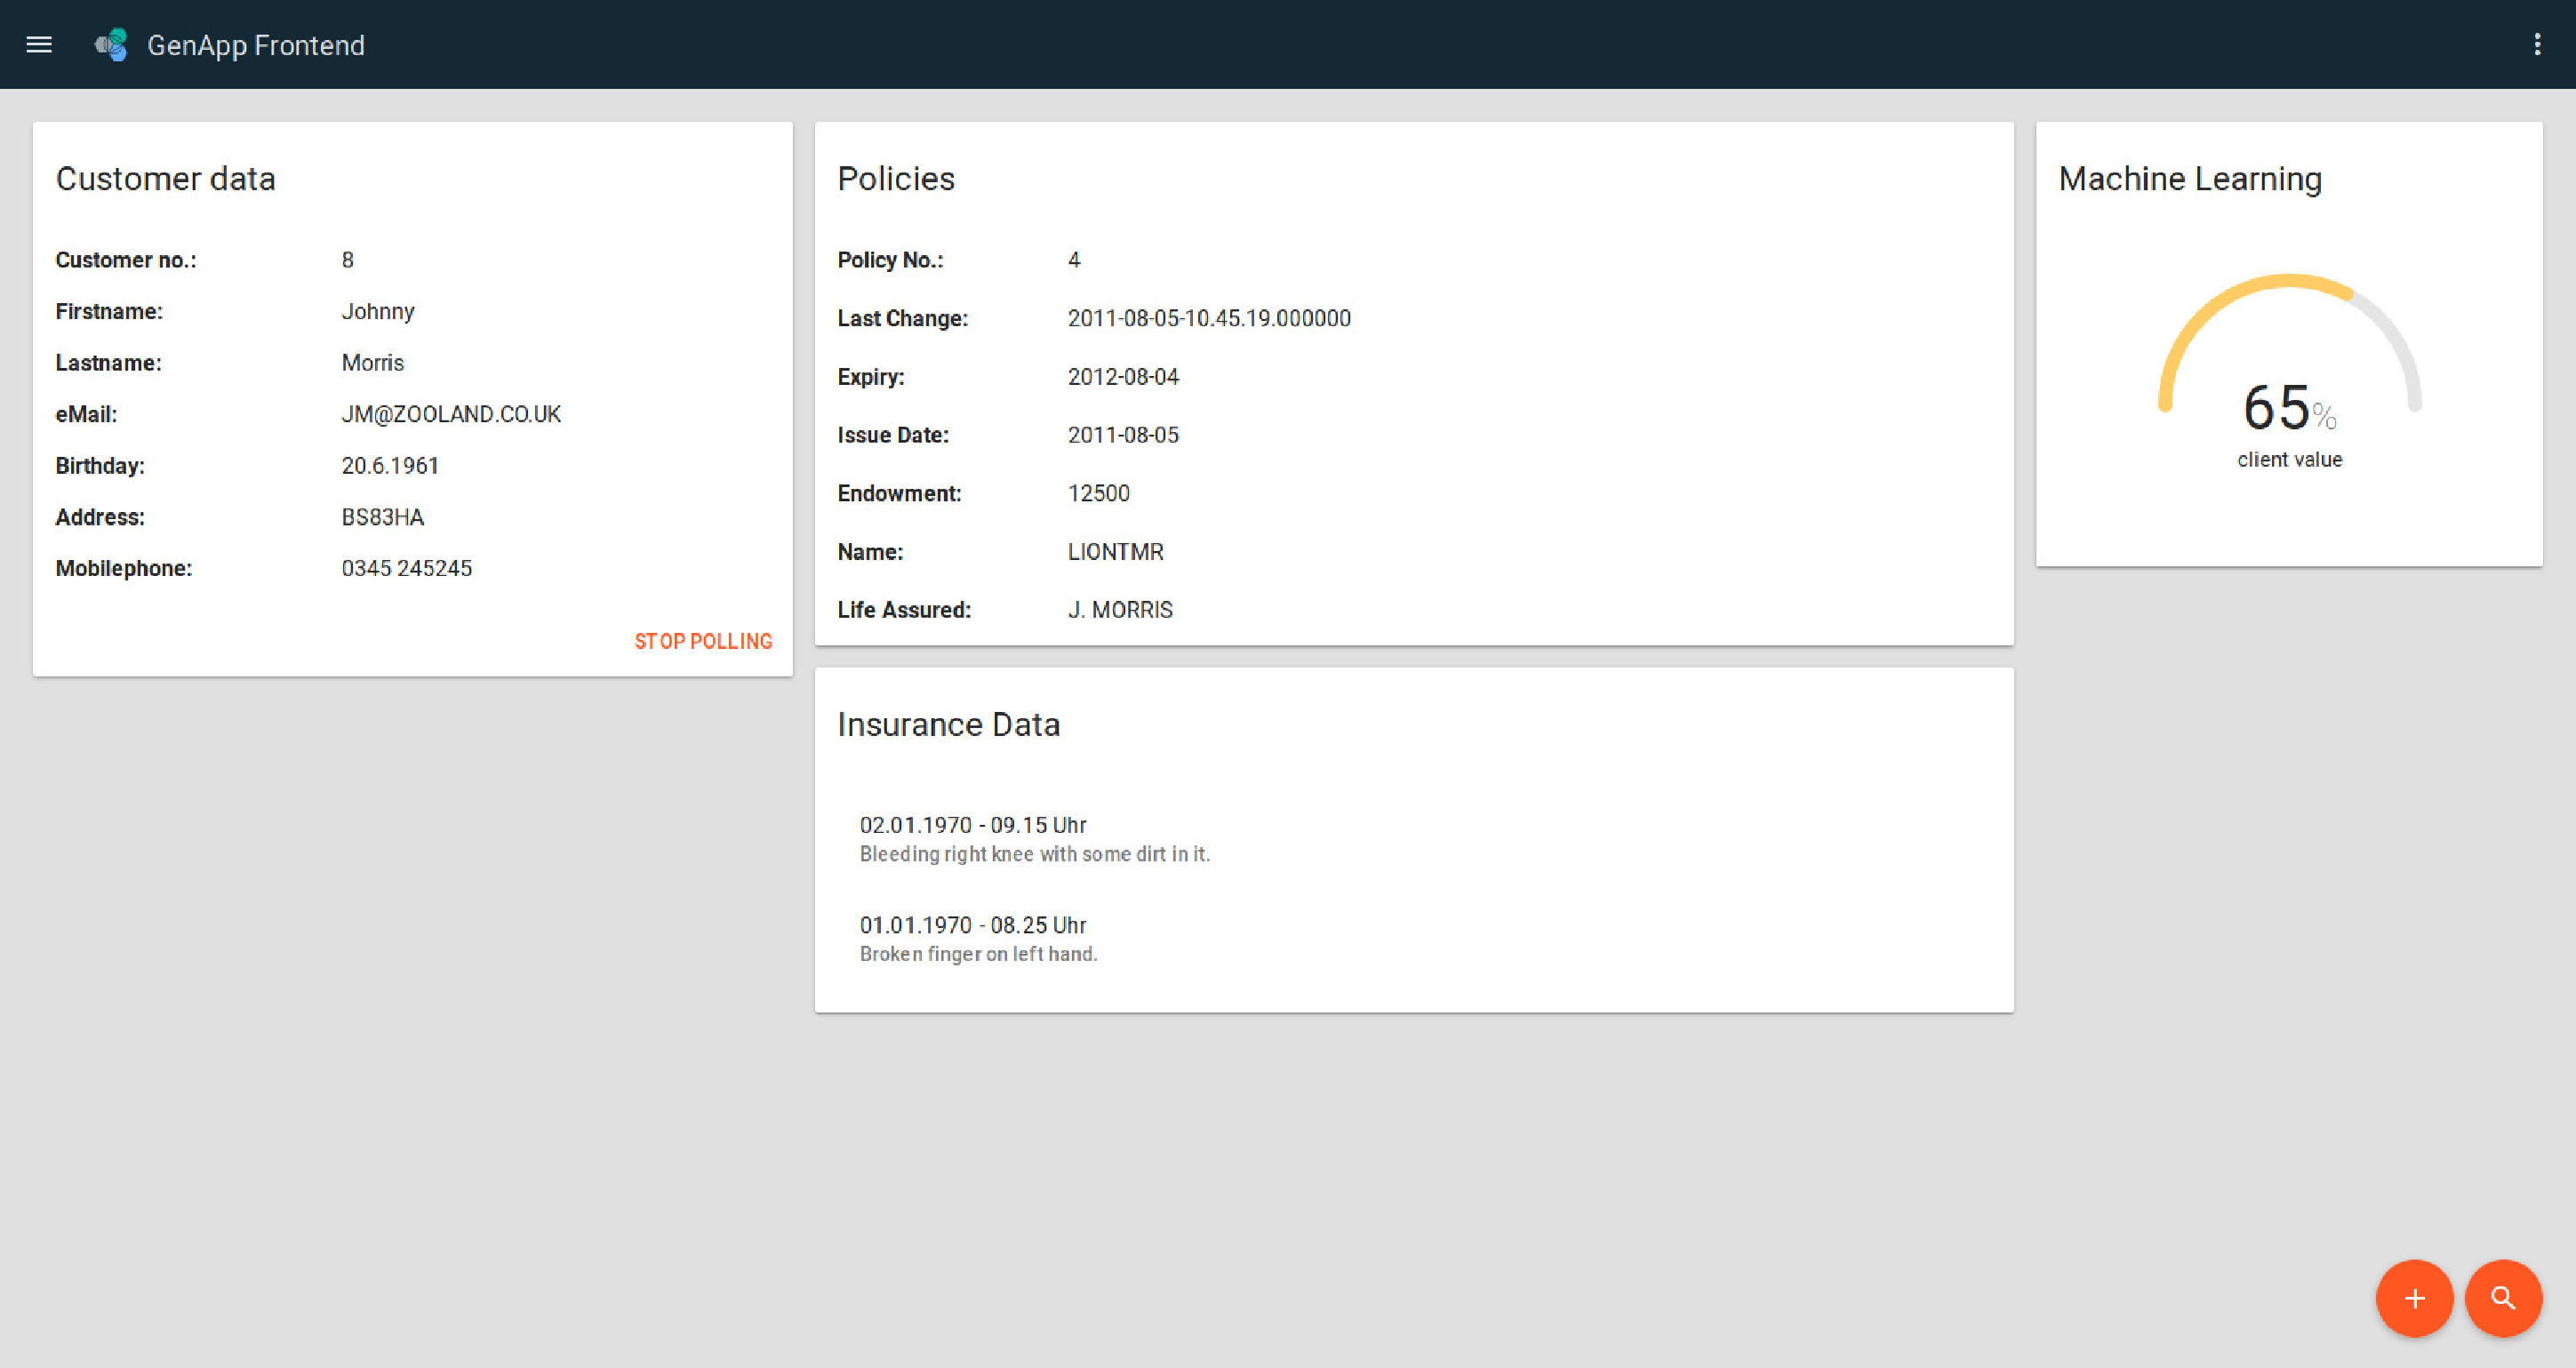
\includegraphics[scale=0.29]{images/kapitel_4/frontend_browser.pdf}
 \caption{Web-Frontend im Browser}
 \label{fig:frontend_browser}
\end{figure}

In Abbildung \ref{fig:frontend_smartphone} auf Seite \pageref{fig:frontend_smartphone} ist das Web-Frontend mit einem
emulierten Smartphone zu sehen. Es handelt sich dabei um eine Auflösung von 360x640 Pixel. In dieser Abbildung
ist ersichtlich, wie das Frontend sich an die Größe des Bildschirms anpasst. In der Größe eines Smartphones würde das
seitliche Menü auch den kompletten sichtbaren Bereich der Webseite überdecken.

Auch die Größe der modalen Fenster ist in der Größe eines Smartphones breiter, damit Daten einfacher eingegeben werden
können.

\begin{figure}[h]
 \centering
   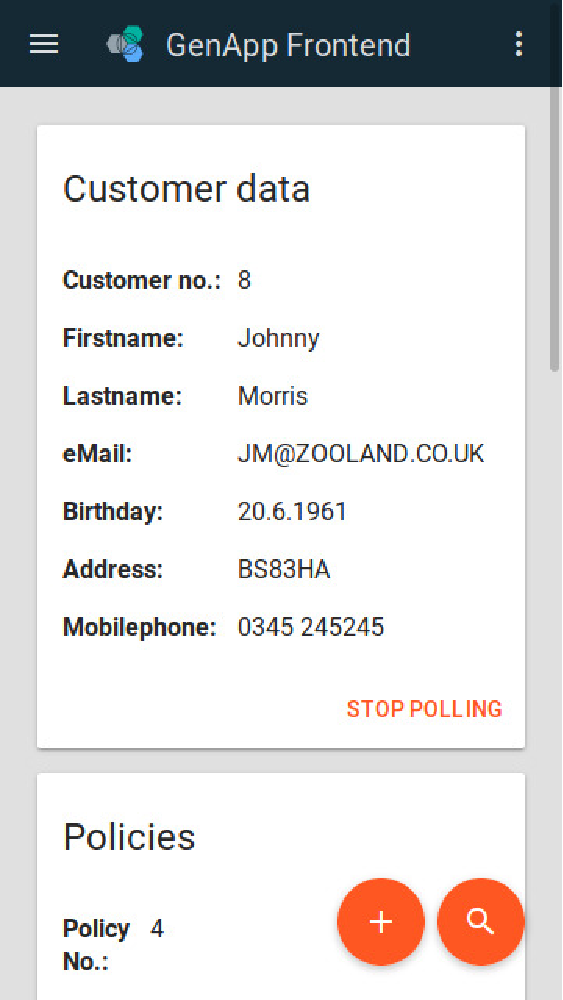
\includegraphics[scale=0.64]{images/kapitel_4/frontend_smartphone.pdf}
 \caption{Web-Frontend im Smartphone}
 \label{fig:frontend_smartphone}
\end{figure}

Die beiden REST-Interfaces des Backends, der Java-Wrapper und der DB2 REST Service, werden in der Umsetzung mit
Angular-Factories angesprochen. Das hat den Vorteil, dass für jedes Backend eine Factory geschrieben wird, die jedem
Controller zur Verfügung gestellt werden kann.

Da nur eine Seite exisitert, wird auch nur ein Angular-Controller benötigt. Dieser kümmert sich um die Übermittlung der
Daten an die \textit{View}, nachdem ein Polling oder eine Suche gestartet wird.

Mit der Cloud Foundry CLI und dem Befehl \path{push} kann das Web-Frontend an Bluemix übertragen und mit der in Kapitel
\ref{subsec:runtime_hinzufügen} auf Seite \pageref{subsec:runtime_hinzufügen} erstellte Cloud Foundry Runtime zur Verfügung
gestellt werden.

Der komplette Quelltext des Frontends ist im zugehörigen GitHub-Repository\footnote{https://github.com/Alienuser/GenAppFrontend}
zu finden. Dieser kann bequem geklont und anschließend in der eigenen Cloud Foundry Runtime zur Verfügung gestellt
werden.

\subsection{Erstellen der Smartphone App}
Da das Web-Frontend nun fertig gestellt ist und über eine Domain mit einem Webbrowser aufgerufen werden kann, können die
Smartphone-Apps erstellt werden, welche das Web-Frontend in einem WebView-Layout laden und darstellen.

Dabei wird dem Layout die Domain übergeben und das Layout kümmert sich selbstständig um die Darstellung der Webseite und
die Interaktion damit.

Da der Aufbau einer Smartphone-App für die verschiedenen Betriebsysteme stark abweicht, wird in den folgenden beiden
Kapiteln die Spezifika der Android- und der iOS-App aufgezeigt. Dabei werden Projekte für die jeweiligen Betriebssysteme
erstellt und die Anwendung entwickelt.

\subsubsection{Android}
Zur Erstellung einer Android-App wird die \path{Android Studio IDE} benötigt. Diese kann kostenlos auf der
Developer-Seite\footnote{https://developer.android.com/studio/index.html} von Google heruntergeladen werden und steht für
Windows, Linux und MacOS zur Verfügung. Android Studio basiert auf der Community Version von
IntelliJ\footnote{https://www.jetbrains.com/idea}.

Für die Verwendung von Android Studio wird eine Installierte \textit{Java-JRE} und das \textit{Java-JDK} benötigt. Die
Java-JRE wird für das Ausführen der IDE genutzt. Das Java-JDK zum Bauen des Quellcodes auf dem Entwicklersystem. Es wird
empfohlen, jeweils die aktuellste Version zu nutzen. Dies ist zur Zeit jeweils Version 8.

Nach der Installation und dem ersten Start von Android Studio muss ein \textit{Android-SDK} sowie ein Emulator heruntergeladen
werden. Dabei werden jeweils die neuesten Versionen ausgewählt. Für das SDK bedeutet das \path{26.0.2} und für den Emulator
\path{Android O} bzw. \path{Android 8}. Mit dem Emulator kann die App später getestet werden. Dabei handelt es sich um ein
vollwertiges Betriebssystem mit allen Möglichkeiten.

Im nächsten Schritt wird ein neues Android-Projekt angelegt. Dazu wird als Name \path{GenAppAndroid} gewählt und ein leeres
Projekt selektiert.

Die Android-App muss im Ordner \path{/res/layout} ein Layout besitzen, welches als Root-Element ein \path{CoordinatorLayout}
besitzt und als Kind-Element ein {WebView} Layout. Diesem wird eine \textit{ID} zugeteilt, damit es aus dem Java-Teil
eindeutlig identifiziert werden kann.

Im Java-Teil wird neben einer \textit{Splashscreen}- noch eine \textit{Main}-Activity hinzugefügt. Erstere soll nach dem
Start der Anwendung das Logo mit entsprechendem Hintergrund anzeigen und erst auf die Main-Activity wechseln, wenn die
Webseite geladen ist.

Die Main-Activity besitzt als unveränderliche Variable die URL des Web-Frontends und konfiguriert in der
\path{onCreate}-Methode das WebView-Layout, damit es JavaScript akzeptiert. Anschließend wird die Webseite im Layout
angezeigt.

Das WebView-Layout, welches von \path{Android-Webkit} erbt, kümmert sich anschließend um die korrekte Darstellung der
Webseite und die Interaktion des Nutzers mit dieser. Mit dem Überschreiben von Funktionen im \path{WebViewClient} kann
das Verhalten des Layouts angepasst werden. So kann zum Beispiel Einfluss auf den Titel oder sogar HTML-Elemente
genommen werden.

In den \path{/res/values} und \path{/res/values-21}-Ordnern werden Farben und Styles definiert. In letzterem lediglich
Styles, die ab Android SDK-Version 21 genutzt werden sollen.

Die Ordner- und Dateistruktur kann in der Abbildung \ref{fig:androidstudio_folder} auf Seite \pageref{fig:androidstudio_folder}
eingesehen werden.

\begin{figure}[h]
 \centering
   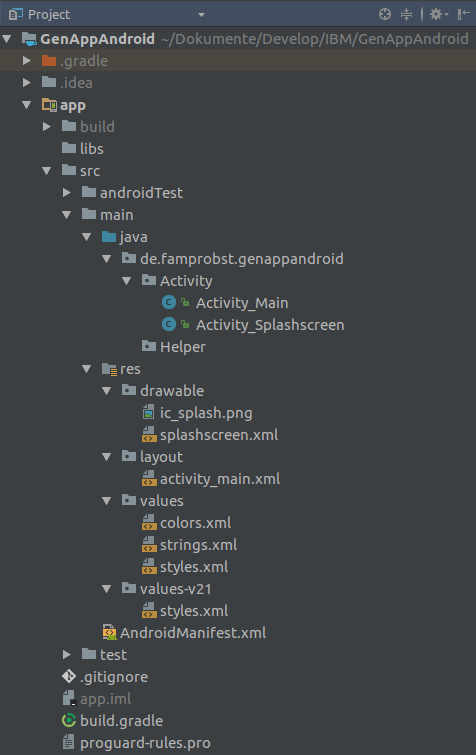
\includegraphics[scale=0.4]{images/kapitel_4/androidstudio_folder.png}
 \caption{Ordner und Dateien in Android Studio}
 \label{fig:androidstudio_folder}
\end{figure}

Im Ordner \path{/res/drawable} ist das Logo der Anwendung (das Bluemix Logo) und auch die Konfiguration des
Splashscreen-Hintergrundes hinterlegt.

Die \path{Manifest.xml}-Datei entählt Informationen und Konfigurationen der Android-App. Zum Beispiel wird in dieser Datei
angegeben, welche Activity beim Start der Anwendung geöffnet werden soll oder welche Styles genutzt werden sollen. Mehr
Informationen dazu gibt es auf den Developer-Seiten\footnote{https://developer.android.com/guide/topics/manifest/manifest-intro.html}
von Android.

In der Abbildung \ref{fig:frontend_smartphone_android} auf Seite \pageref{fig:frontend_smartphone_android} ist die fertig
entwickelte Android-App auf einem Smartphone-Emulator zu sehen.

\begin{figure}[h]
 \centering
   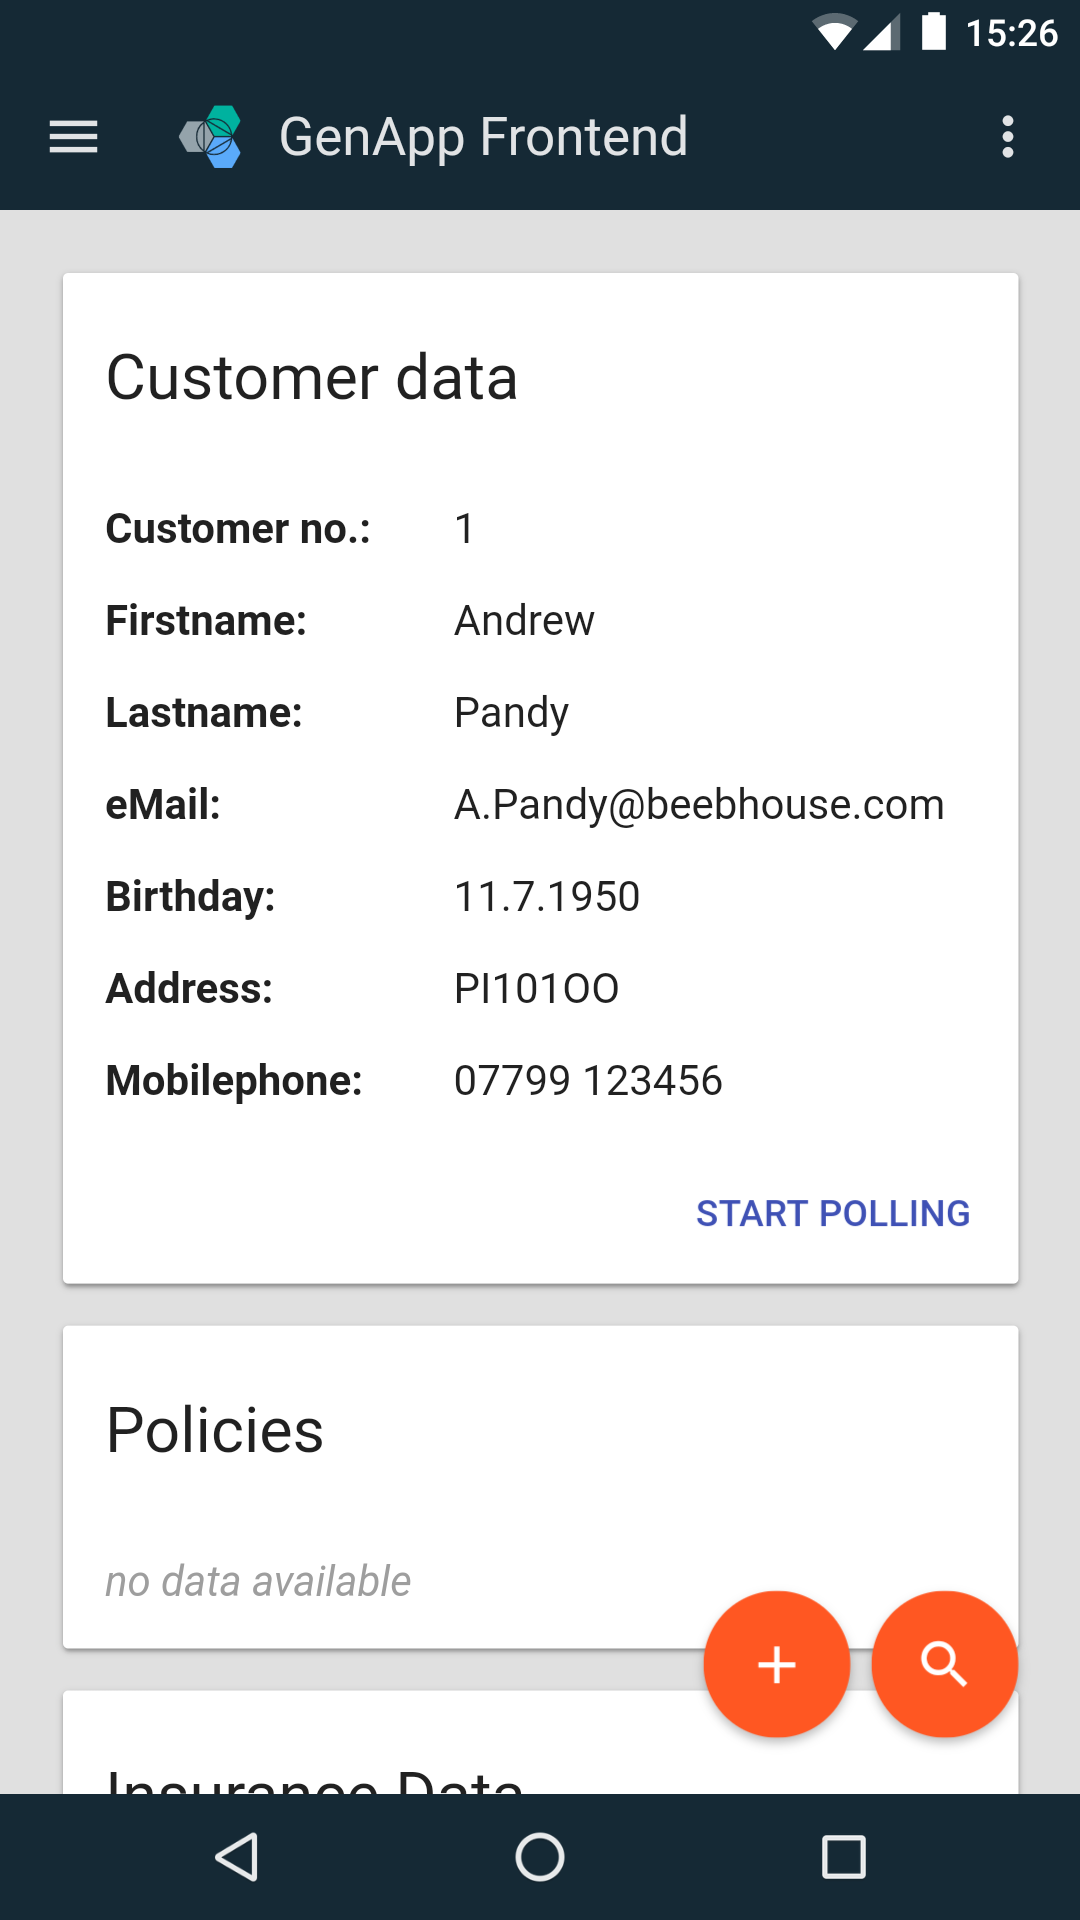
\includegraphics[scale=0.19]{images/kapitel_4/frontend_smartphone_android.png}
 \caption{Android-App im Smartphone-Emulator}
 \label{fig:frontend_smartphone_android}
\end{figure}

In dieser Abbildung ist sichtbar, dass die Android-Styles Einfluss auf die Darstellung der Menüpunkte (am unteren Rand)
und die Farbe des Toolbar nehmen kann. Beide werden in der selben Farbe wie der Header im Web-Frontend dargestellt.

In der Abbildung \ref{fig:frontend_tablet_android} auf Seite \pageref{fig:frontend_tablet_android} wird die Anwendung in
einem Tablet-Emulator gezeigt. Im Vergleich der beiden Screenshots ist gut zu sehen, dass sich das Frontend den Gegebenheiten
wie zum Beispiel Bildschirmgröße gut anpasst.

\begin{figure}[h]
 \centering
   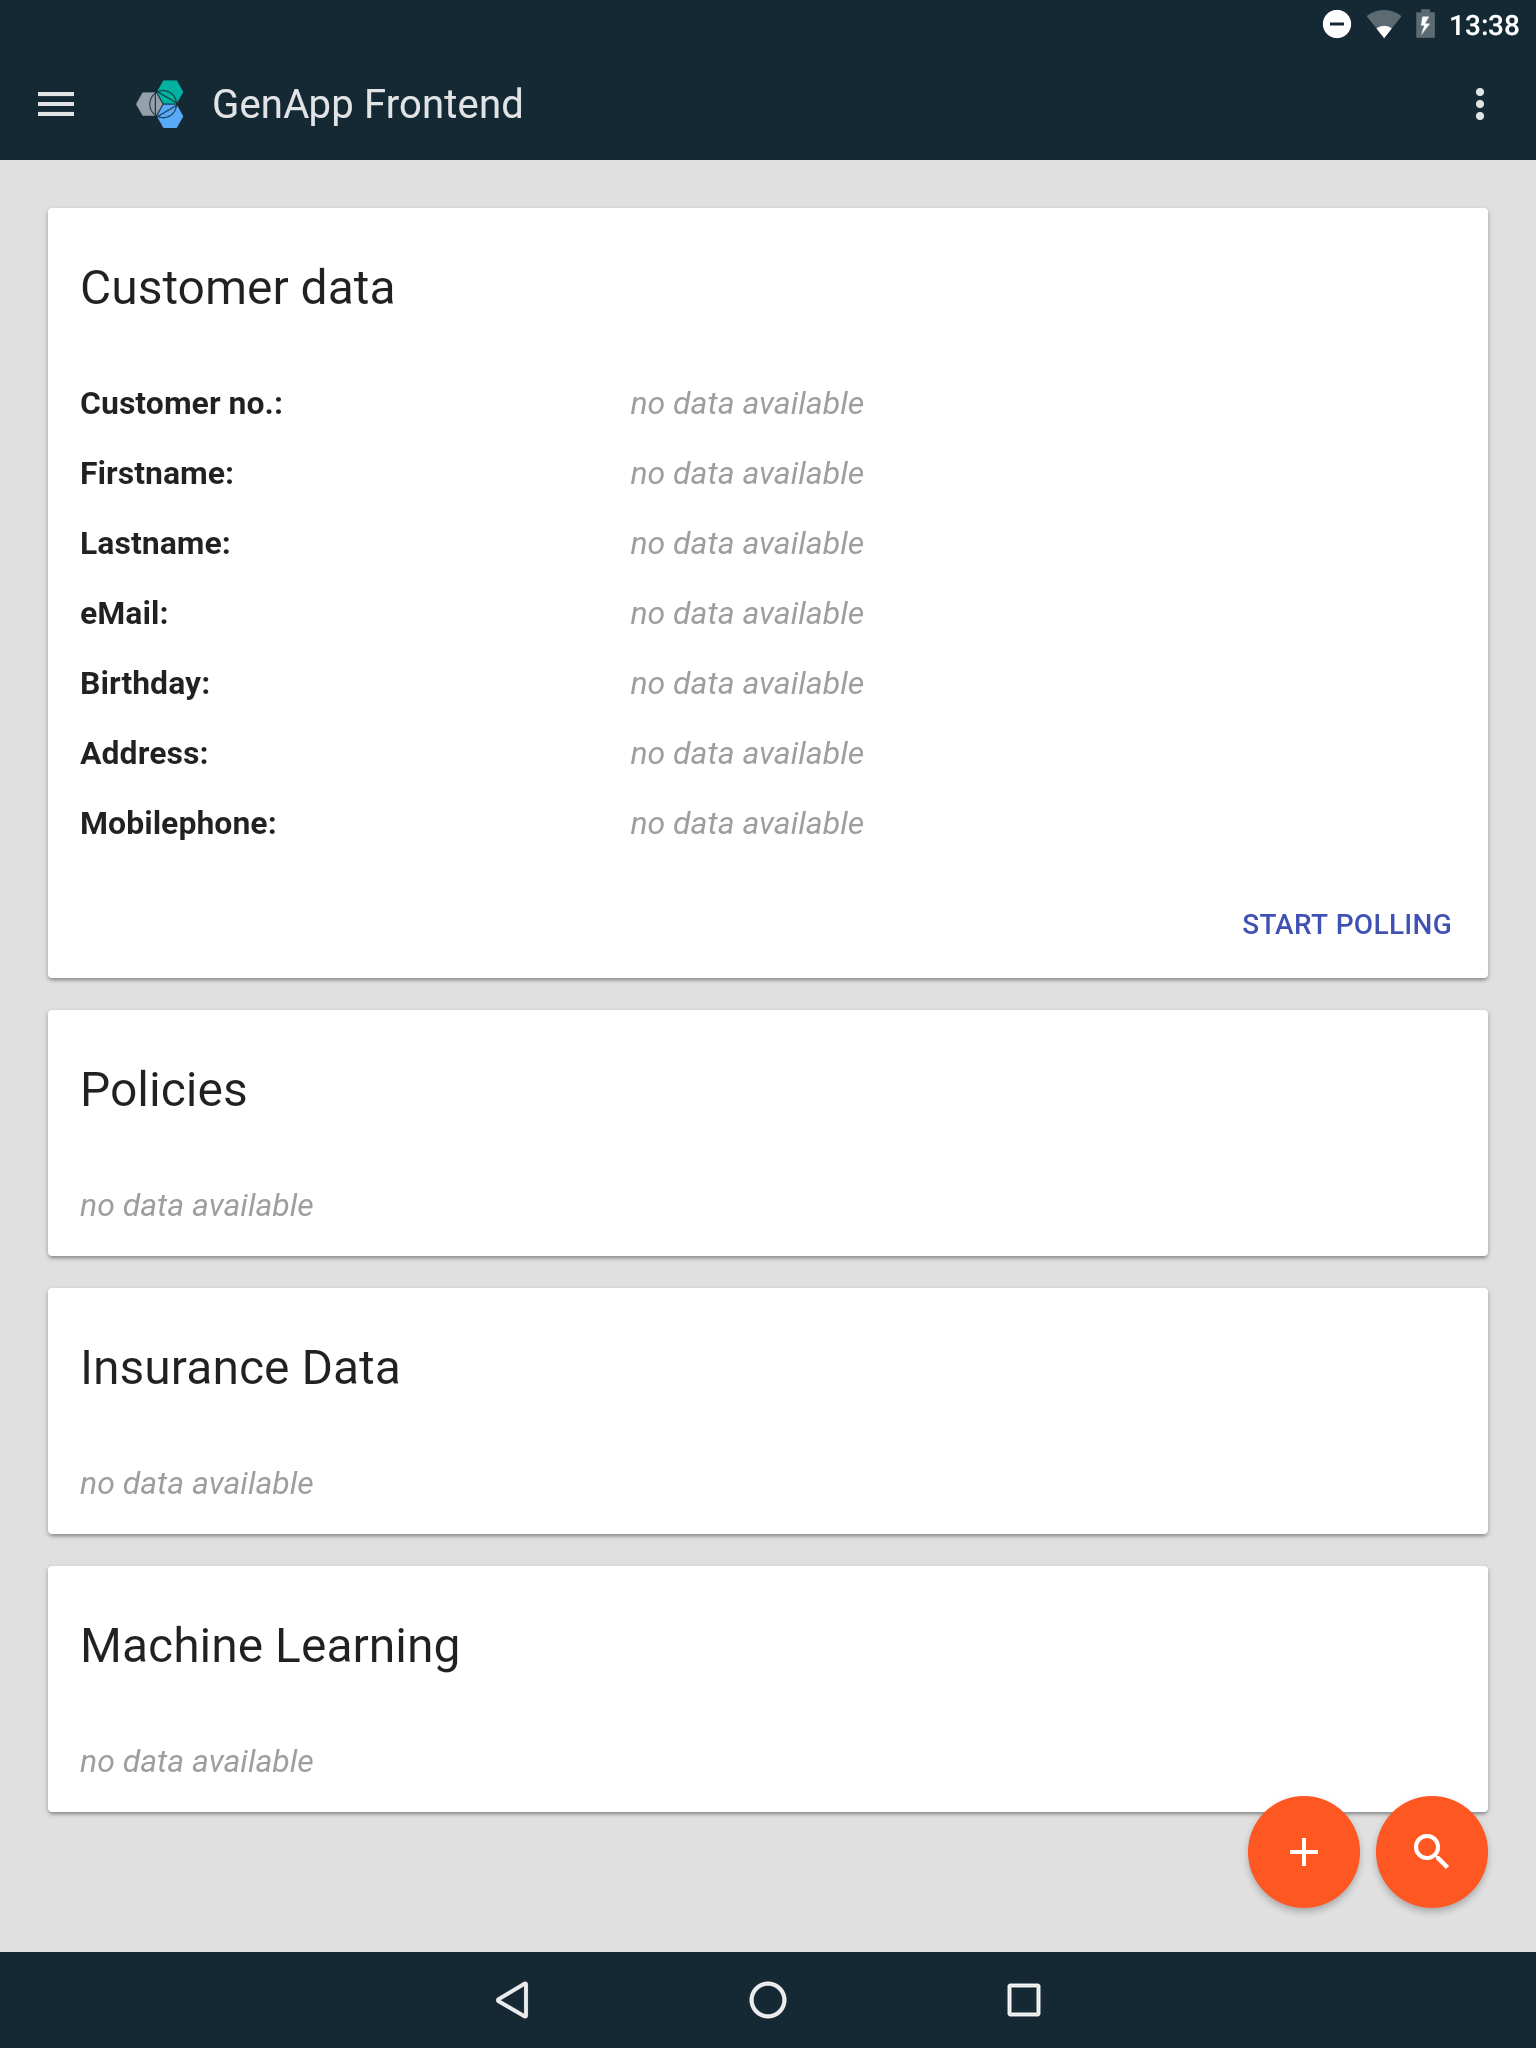
\includegraphics[scale=0.18]{images/kapitel_4/frontend_tablet_android.png}
 \caption{Android-App im Tablet-Emulator}
 \label{fig:frontend_tablet_android}
\end{figure}

Der Quelltext der Android-App kann im GitHub-Repository\footnote{https://github.com/Alienuser/GenAppAndroid} eingesehen
werden.

Es ist möglich das GitHub-Projekt direkt in Android Studio zu klonen und als Projekt zu nutzen. Dazu muss beim Start von
Android Studio \path{Check out project from version control} ausgewählt werden, worauf die GitHub-URL eingegeben werden
muss.

Das Projekt wird nun automatisch angelegt und der benötigte Gradle-Wrapper heruntergeladen. Anschließend wird das Projekt
direkt gebaut und die benötigten Abhängigkeiten heruntergeladen. Anschließend kann die App in einem beliebigen Emulator
getestet werden.

Die Android-App ist nun fertig entwickelt und kann exportiert werden. Dazu wird eine \textit{Signing}-Datei erstellt
mit welcher es möglich ist, die Anwendung auch in den Play-Store zu laden. Alternativ kann die exportierte
\textit{Android Package}-Datei (kurz APK) auch auf echten Geräten installiert werden.

\clearpage
\newpage

\subsubsection{iOS}
Um eine App für iOS Geräte zu entwickeln, wird die kostenlose IDE \path{XCode} benötigt. Diese steht lediglich MacOS-Geräten
zur Verfügung und kann auf der Developer-Seite\footnote{https://developer.apple.com/xcode} von Apple heruntergeladen werden.

Somit ist das Schreiben, Kompilieren und Testen einer iOS-App unter XCode nur unter MacOS möglich, was eine große
Einschränkung darstellt.

Nach der Installation wird in XCode anschließend ein neues Projekt angelegt. Die Art des Projektes ist \path{SingleViewApp}
und der Name ist zum Beispiel \path{GenAppiOS}. In Abbildung \ref{fig:xcode_overview} auf Seite \pageref{fig:xcode_overview}
ist das erstellte Projekt in XCode zu sehen. Der Emulatoren und die verschiedenen SDKs werden automatisch installiert.

\begin{figure}[h]
 \centering
   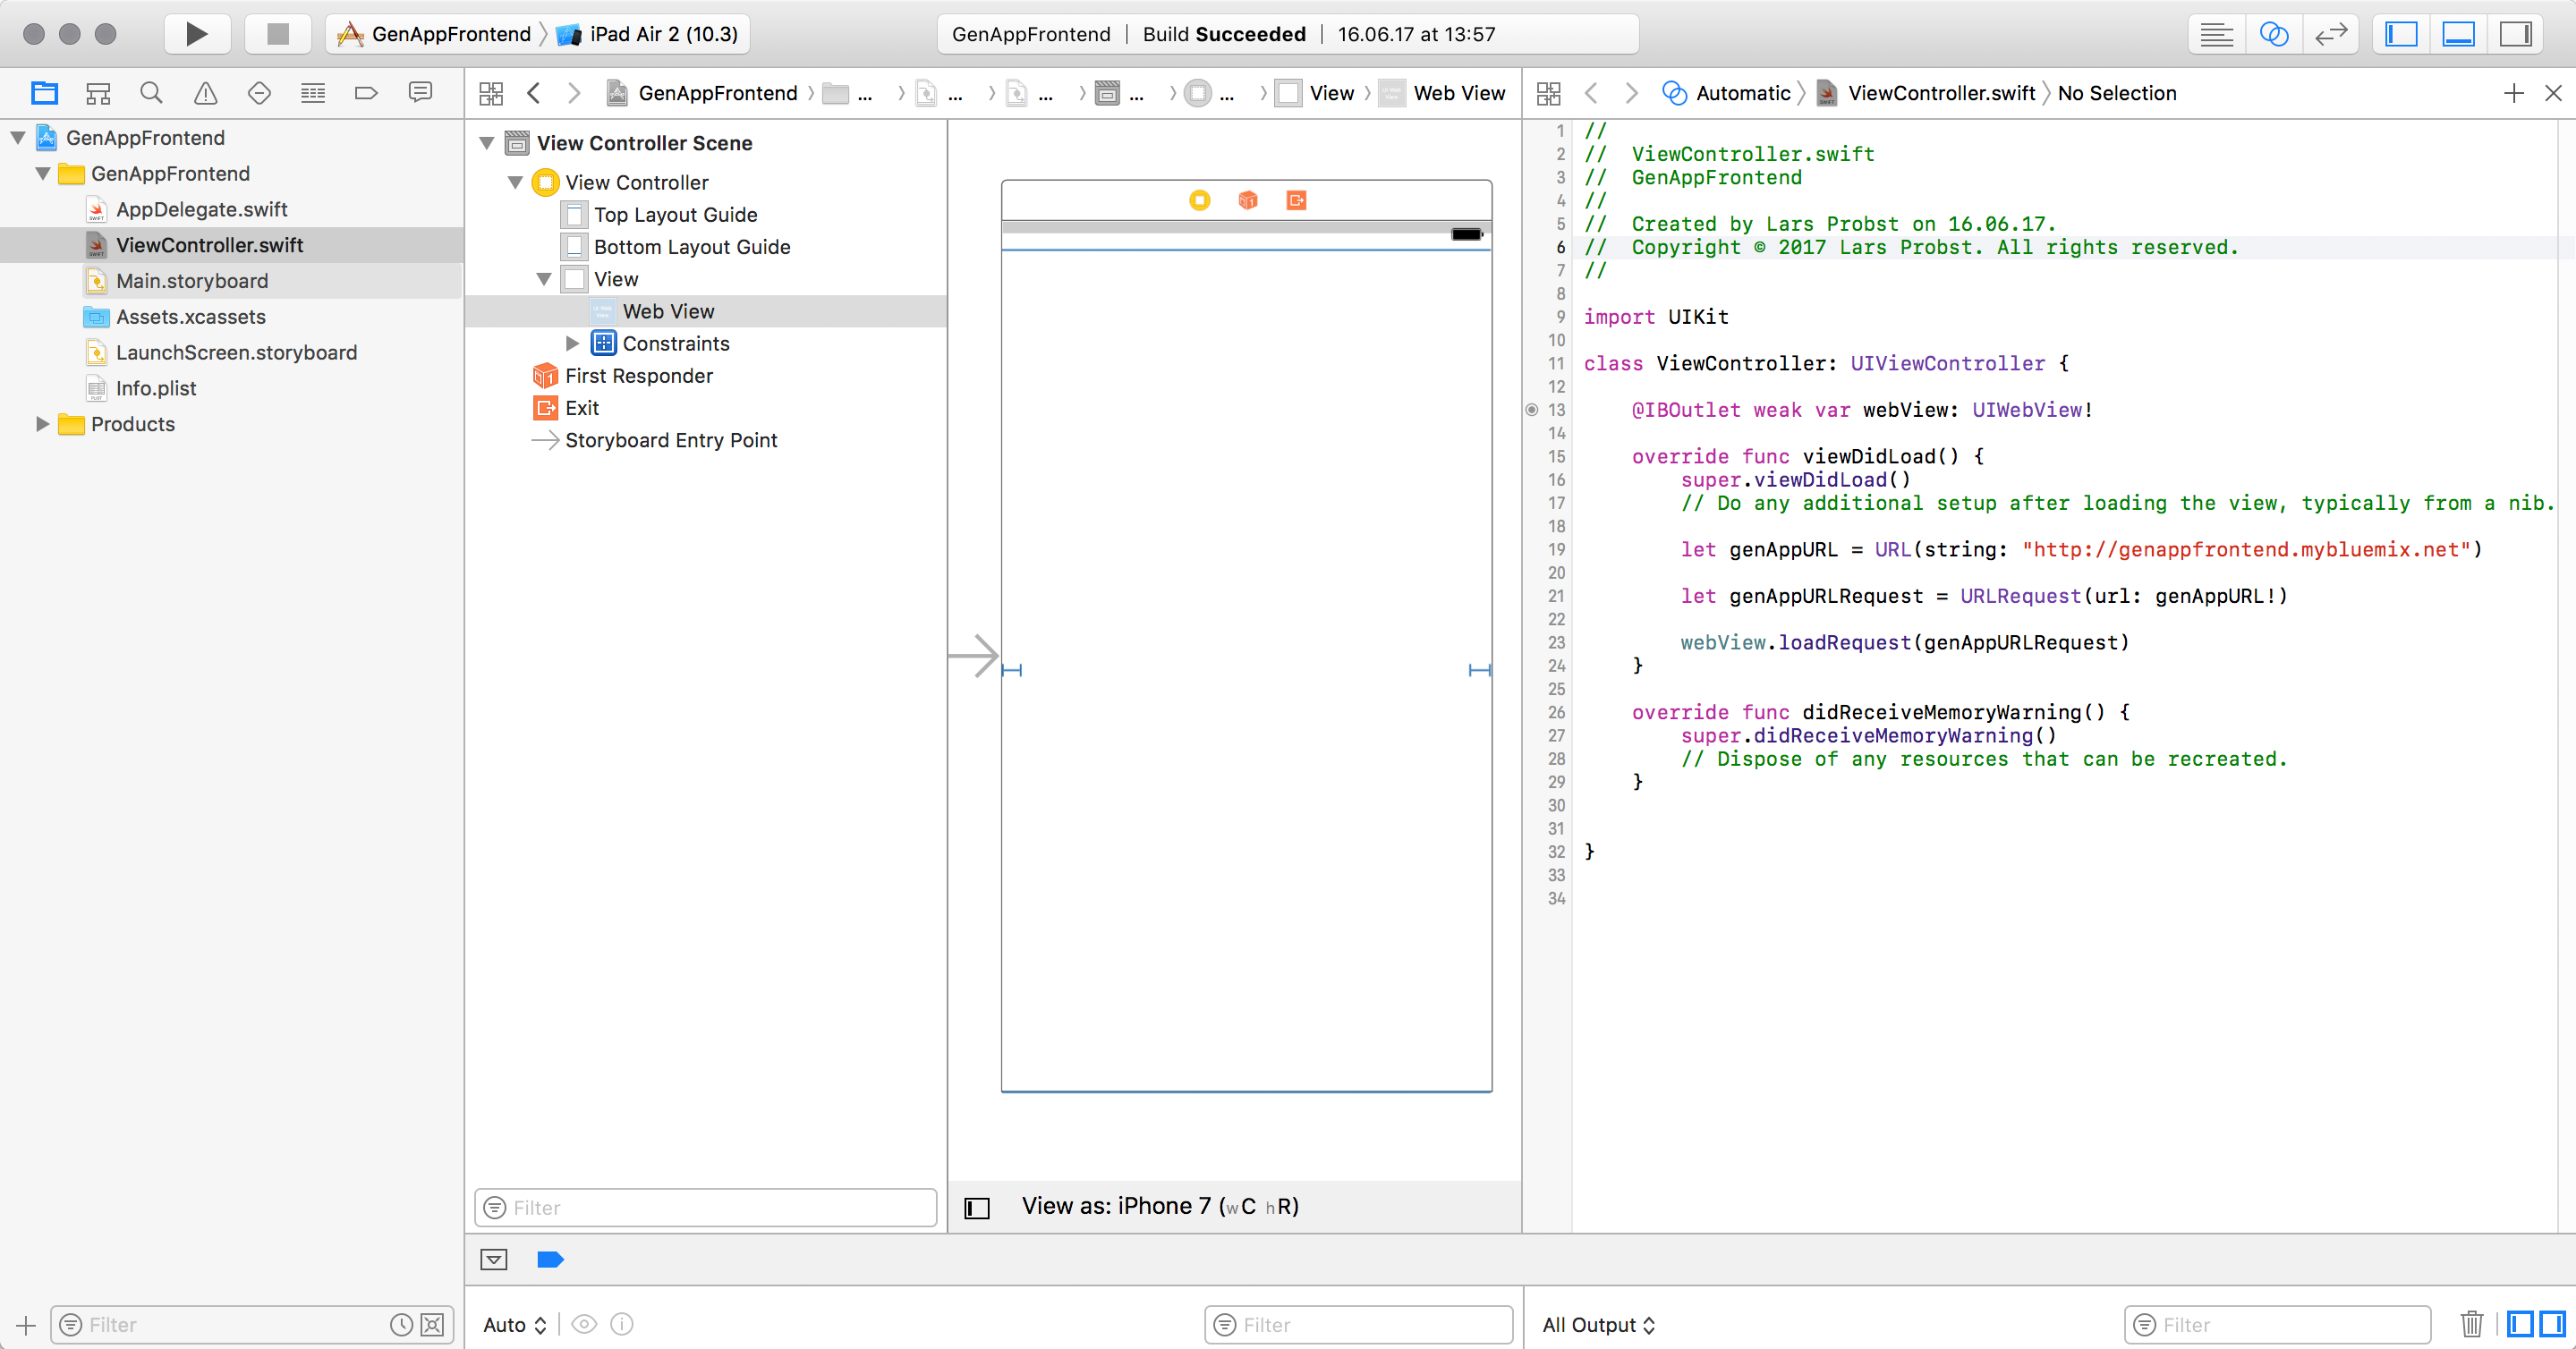
\includegraphics[scale=0.26]{images/kapitel_4/xcode_overview.png}
 \caption{Übersicht von XCode}
 \label{fig:xcode_overview}
\end{figure}

Bei den beiden \path{.swift}-Dateien handelt es sich um die ausführbaren Klassen innerhalb der Anwendung. Ihn ihnen wird
die Logik entwickelt.

Dabei wird in der \path{ViewController}-Datei die genutzte View konfiguriert und, wie in der Abbildung zu sehen, zum
Beispiel dem WebView-Layout die URL des Web-Frontends übergeben.

In der \path{AppDelegate}-Datei wird der Lifecycle der Anwendung definiert. So wird dort festgelegt, dass der genutzte
Controller das \path{LaunchScreen}-Storyboard zugeteilt bekommt.

Die \path{.storyboard}-Dateien sind für die Darstellung der einzelnen Seiten und Menüs zuständig. Davon wird in diesem
Projekt nur eine benötigt, welche das Web-Frontend darstellen kann.

Als Letztes wird die \path{.plist}-Datei für die Konfiguration der Anwendung benötigt. Sie ist ähnlich der
Android-Manifest-Datei.

In Abbilung \ref{fig:xcode_folder} auf Seite \pageref{fig:xcode_folder} ist eine Übersicht der Ordnerstruktur in XCode
abgebildet. Dort sind alle genutzten Dateien sichtbar.

\begin{figure}[h]
 \centering
   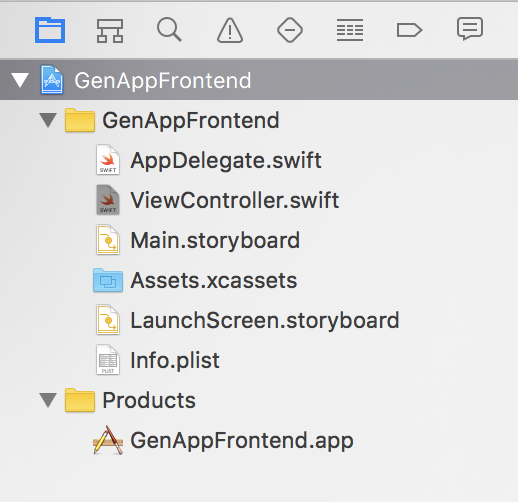
\includegraphics[scale=1]{images/kapitel_4/xcode_folder.png}
 \caption{Ordner und Dateien in XCode}
 \label{fig:xcode_folder}
\end{figure}

Die Plist-Datei (Property List Files) beinhaltet die Konfiguration der Anwendung. So wird hier zum Beispiel eingestellt,
ab welcher Version die Anwendung zur Verfügung stehen soll und ob es zum Beispiel Einschränkungen in der Ausrichtung der
App geben soll. Außerdem wird der Name der Anwendung und das verwendete Icon definiert.

Anschließend wird im Storyboard, der View, ein WebView-Layout angelegt. Dieses wird mit der Programmiersprache Swift dann
angesprochen und konfiguriert. Ähnlich der Android-App werden Informationen wie Domain oder Anzeigegröße übergeben und das
Layout kümmert sich eigenständig um das Laden, das Darstellen und die Interaktion mit dem Nutzer der Webseite.

Nach einem Klick auf \path{Run} (kleiner schwarzer Play-Button) in XCode, kann der Emulator ausgewählt werden, mit welchem
die Anwendung gestartet werden soll. In der Abbilung \ref{fig:frontend_smartphone_ios} auf Seite
\pageref{fig:frontend_smartphone_ios} ist die Anwendung im Smartphone Emulator mit der neuesten iOS Version zu sehen.

\begin{figure}[h]
 \centering
   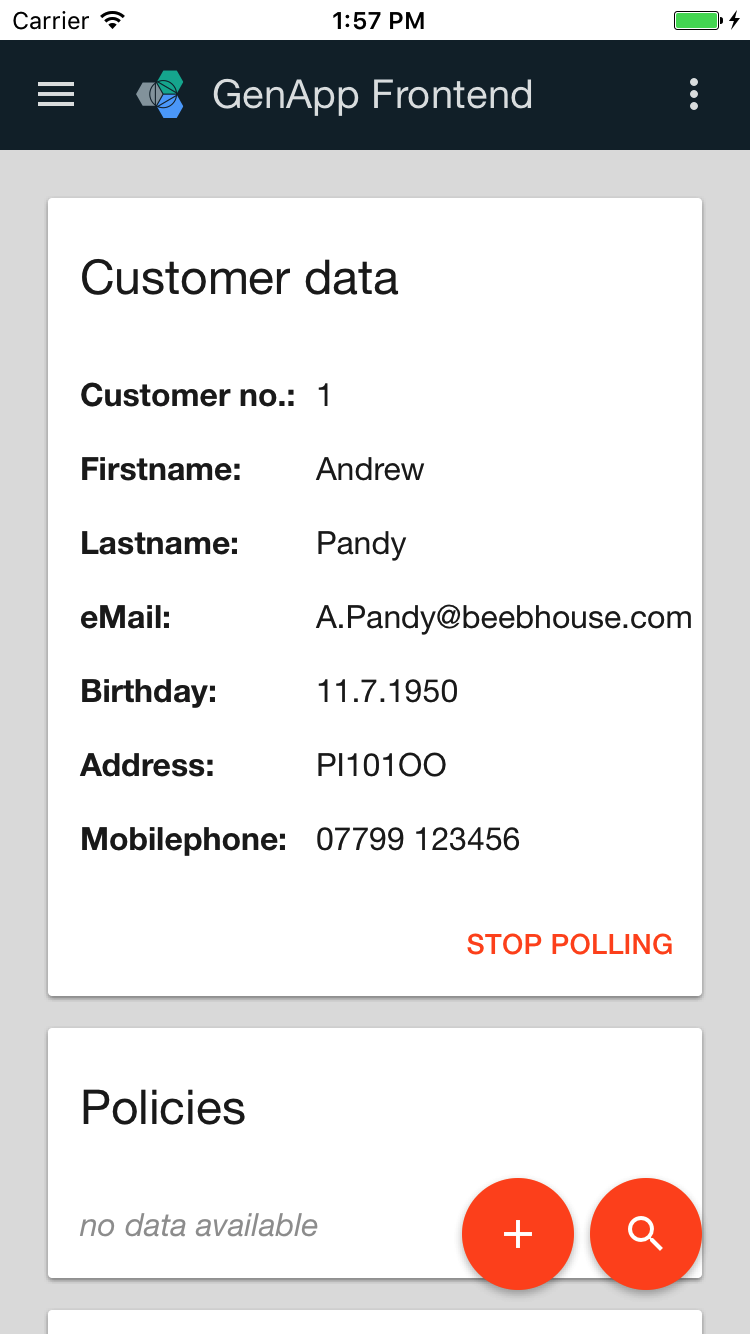
\includegraphics[scale=0.28]{images/kapitel_4/frontend_smartphone_ios.png}
 \caption{iOS-App im Smartphone-Emulator}
 \label{fig:frontend_smartphone_ios}
\end{figure}

Die Abbildung \ref{fig:frontend_tablet_ios} auf Seite \pageref{fig:frontend_tablet_ios} hingegen zeigt die Anwendung in
einem Tablet-Emulator mit ebenfalls der neuesten iOS Version.

Auch in diesen beiden Version zeigt sich, dass sich das Web-Frontend gut an die Displaygrößen anpasst. Dies ist gewünscht,
da sonst eine Interaktion mit der Webseite nicht bzw. schwer möglich ist.

Leider ist es unter iOS nicht möglich die Farbe der Titleleiste einzustellen, sodass sie hier einfach weiß, wie vom System
definiert, bleibt. Ansonsten würde sich die Titelleiste besser in das Gesamtlayout eingliedern.

\begin{figure}[h]
 \centering
   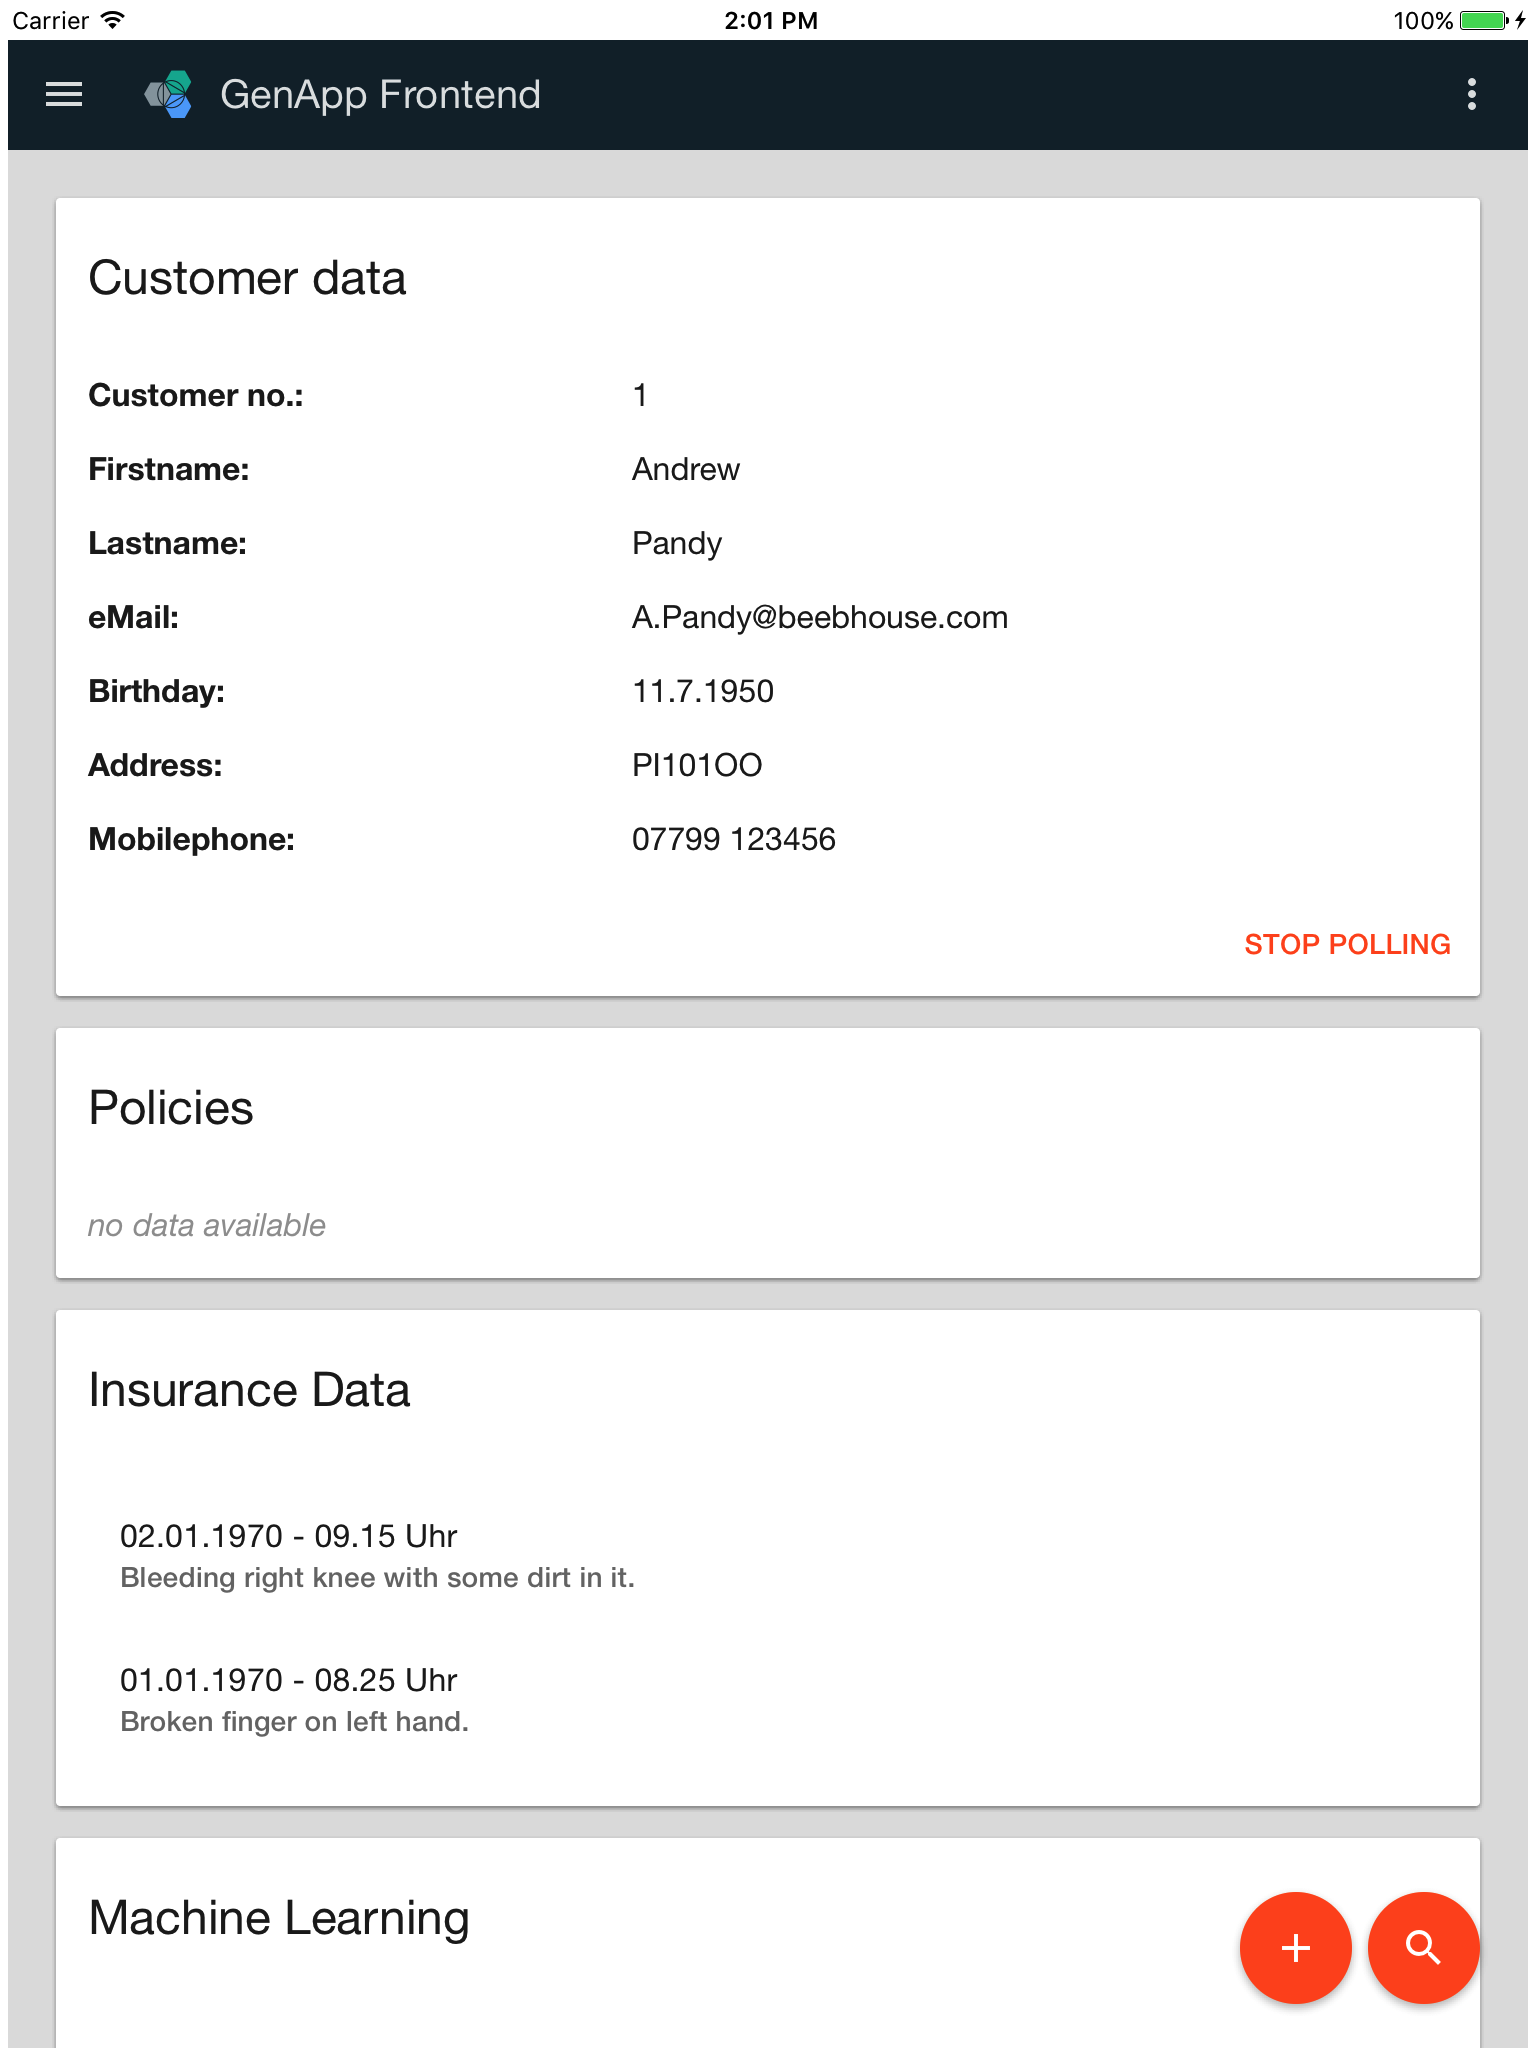
\includegraphics[scale=0.2]{images/kapitel_4/frontend_tablet_ios.png}
 \caption{iOS-App im Tablet-Emulator}
 \label{fig:frontend_tablet_ios}
\end{figure}

Die iOS-App kann nun exportiert und nach Bedarf auf echten Geräten installiert werden. Alternativ ist es auch möglich
die Version in den App-Store zu laden.
\section{Abschluss}
An diesem Punkt ist die prototypische Implementierung der aufgebauten Hybrid-Cloud-Architektur abgeschlossen. Es sind
alle benötigten Anwendungen implementiert und durch ausprobieren, manuell getestet worden.

Im weiteren Verlauf der Arbeit (Kapitel \ref{cha:qualitaetssicherung} ab Seite \pageref{cha:qualitaetssicherung}) werden
darüber hinaus automatisierte Tests geschrieben, welche die Funktion der einzelnen Komponenten stehts überprüfen sollen.

In Abbildung \ref{fig:architektur_gesamtf} auf Seite \pageref{fig:architektur_gesamtf} ist abschließend eine Gesamtübersicht
aller Anwendungen und der Hybrid-Cloud-Architektur zu sehen. Die Abbildung zeigt auch, welche Komponenten miteinander
kommunizieren können und wie einzelne Komponenten zusammenhängen.

\begin{figure}[h]
  \centering
    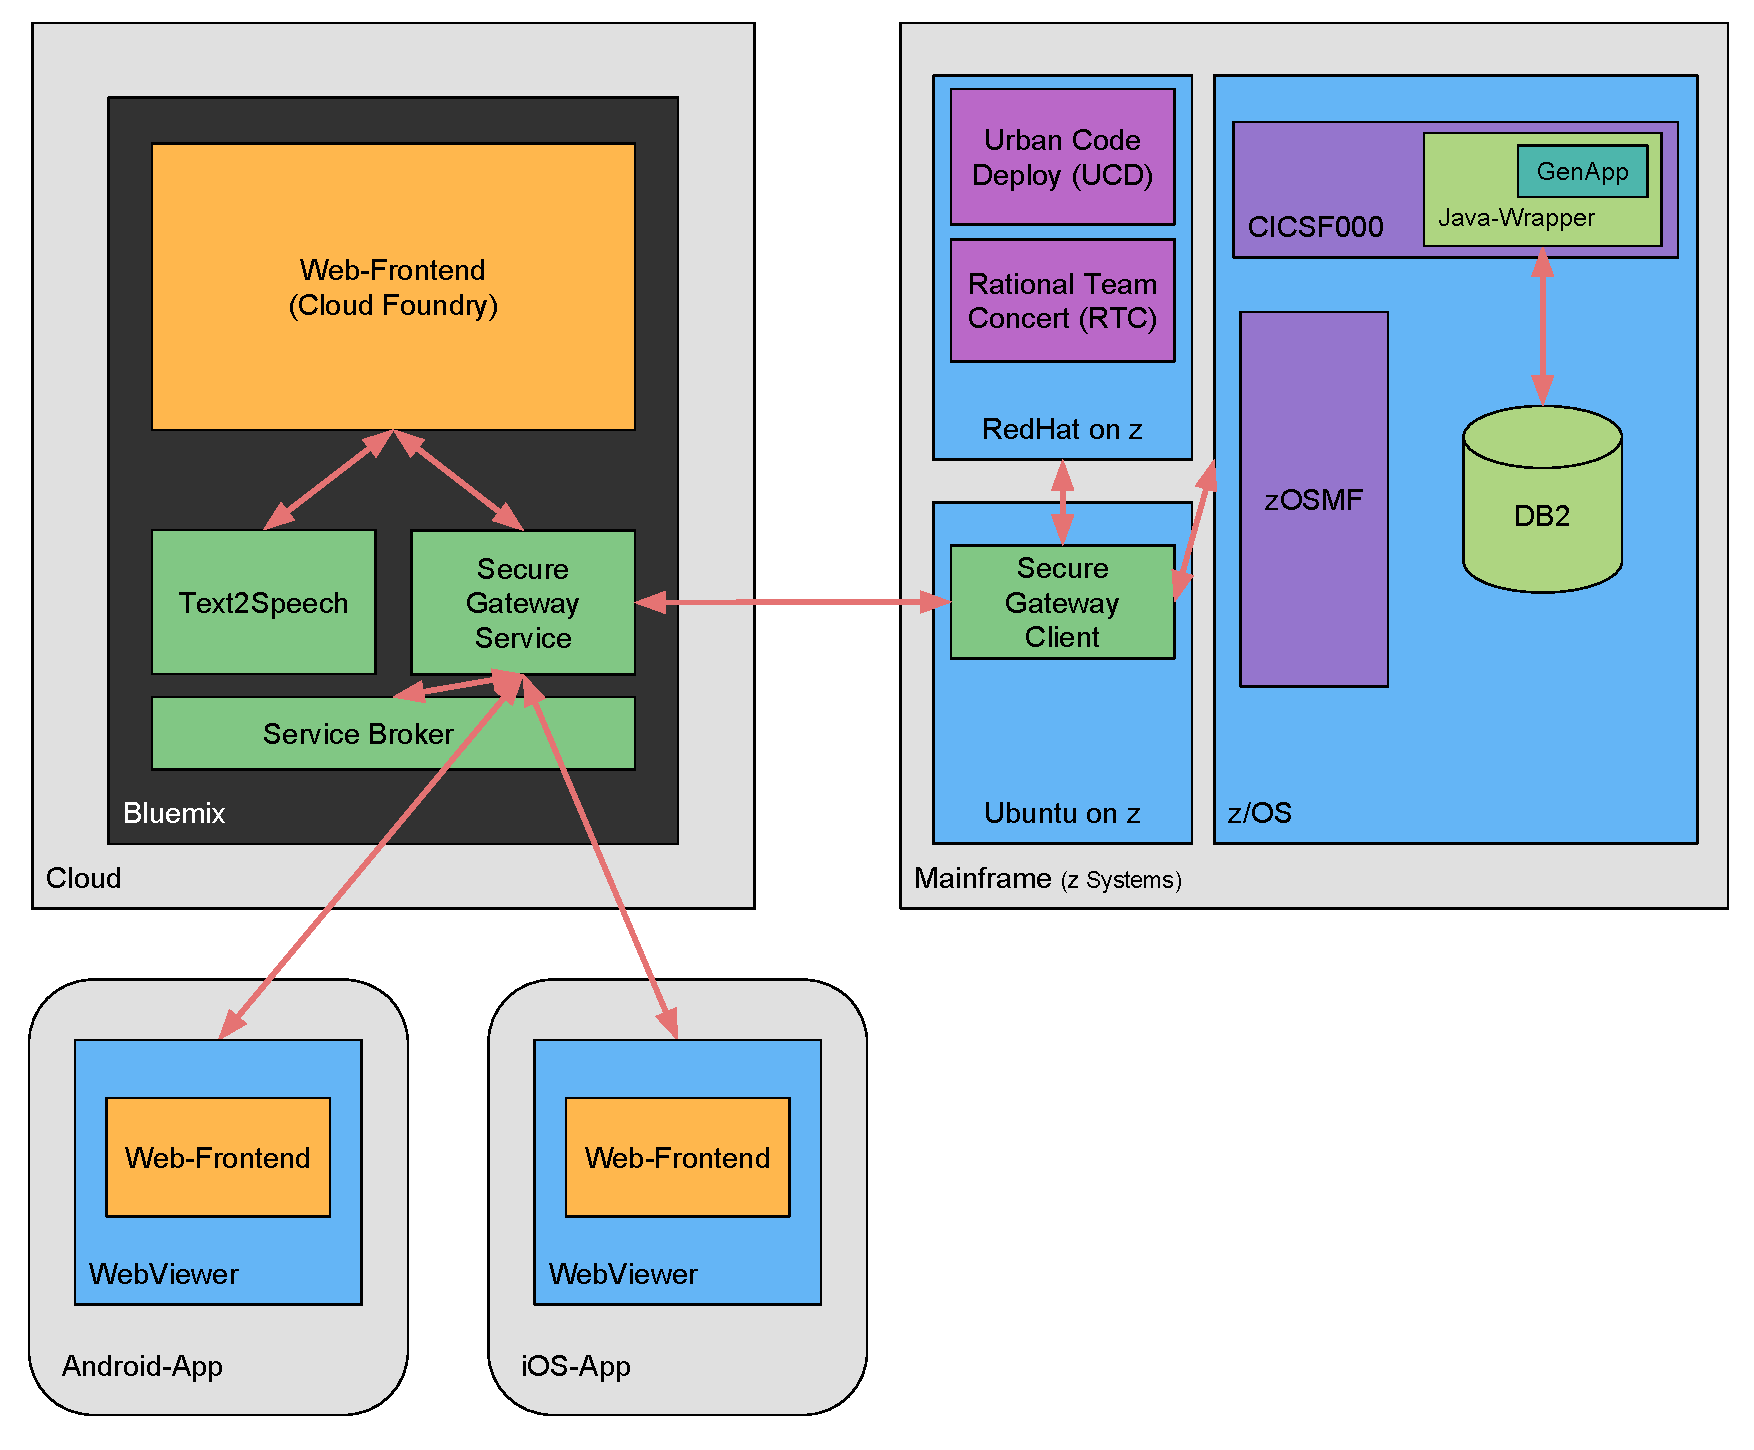
\includegraphics[scale=0.5]{images/kapitel_4/architektur_gesamt.pdf}
  \caption{Gesamtübersicht der Anwendung}
  \label{fig:architektur_gesamtf}
\end{figure}
\chapter{Qualitätssicherung}
\label{cha:qualitaetssicherung}
Um bei der Entwicklung von Applikationen eine hohe Qualität sicherstellen zu können und die Entwicklung zu beschleunigen,
müssen automatisierte Tests geschrieben werden (siehe mehr dazu unter \cite{online_quali_automatisiertetests}).

In diesem Kapitel wird erklärt, warum automatisierte Tests wichtig sind und wie in der Zukunft getestet werden muss, wenn
in einer Hybrid-Cloud-Umgebung gearbeitet werden soll.

Auch werden Tests für die jeweiligen Teilprogramme entwickelt und in den Buildprozess eingebunden.

\section{Allgemein}
Ein großer Vorteil der Cloud ist die schnelle und agile Entwicklung, die dort möglich ist. Problematisch ist es, wenn
zwar in schnelleren und kürzeren \textit{Sprints}, Versionen an den Geschäftspartner oder den Endkunden herausgegeben
werden können, diese aber gar nicht oder nur teilweise funktionieren.

Ein großes Ziel vieler Unternehmen ist die \glqq \textit{Time to Market}\grqq~zu reduzieren. Dennoch gilt die Regel,
dass nur Software, die vom Kunden genutzt werden kann, dem Unternehmen Geld bringt.

Eine Möglichkeit, diesem entgegen zu wirken und eine höhere Qualität der Software zu erreichen, ist der Aufbau von
automatisierten Tests. Frei nach dem Motto \glqq \textit{fail early and fail often}\grqq~wird die Software in nahezu
allen Funktionen vor dem eigentlichen Deployment getestet.

Der Testdurchlauf kann beliebig häufig neugestartet und wiederholt werden und das auch immer mit unterschiedlichen
Programmversionen.

Neben vielen weiteren haben automatisierte Tests den Vorteil, dass sie zu jeder Tages- und Nachtzeit durchlaufen
können und keine menschliche Person daneben sitzen muss, um den Test zu überprüfen. In der Regel wird die verantwortliche
Person nach einem Testdurchlauf über das Ergebnis benachrichtigt und kann dann eingreifen.

Allerdings sind automatisierte Tests nicht immer und für jede Anwendung geeignet. Michael Lüttel von der Deutschen
Flugsicherung sagte auf der iqnite-Konferenz in Düsseldorf \glqq Automatisierung macht nur dann Sinn, wenn sie mehr Aufwände
einspart als sie selbst erzeugt.\grqq\footnote{https://www.qz-online.de/news/uebersicht/nachrichten/vor-und-nachteile-von-automatisierten-software-tests-890130.html}.

\section{COBOL-Anwendung}
Für Unit Tests in COBOL hat, neben IBM, die Firma Compuware das Program
\path{Topaz for Total Test}\footnote{http://www.compuware.com/en\_us/products/topaz-for-total-test.html} entwickelt.
Dabei handelt es sich um ein Testprogramm, um Testfälle zu definieren und diese bei Quellcodeänderungen automatisch
auszuführen.

Da die vorliegende COBOL-Anwendung nicht komplett selbstgeschrieben wurde und nur die Schnittstellen mittels IBM Application
Discovery definiert wurden, werden keine Tests geschrieben.

Es wird lediglich die definierte Schnittstelle getestet indem die richtigen Parameter an die Anwendung geschickt werden
um anschließend zu überprüfen, ob die Daten richtig in die Datenbank geschrieben, abgeändert oder gelesen wurden.

Diese Tests werden am Anfang durchgeführt, und da sich die COBOL-Anwendung weder ändert noch angepasst wird, müssen sie
nicht wiederholt werden. Eine Einbindung in einen Buildprozess ist deshalb nicht nötig.

\section{Frontend}
Da es sich beim Frontend um eine Applikation auf Basis von HTML, CSS und JavaScript handelt und diese im Browser angezeigt
werden, werden für das Frontend Headless-Browser-Tests erstellt.

Bei Headless-Browser-Tests handelt es sich um Tests, welche die Webseite mit Hilfe einem vorgegebenem Pfad virtuell
durchklicken und das resultierende DOM-Objekt mit der Vorgabe vergleichen.

Bei der Überprüfung des DOM-Objektes kann lediglich ein kleiner Teil vorgegeben werden, welcher überprüft werden soll. So
ist es zum Beispiel möglich zu testen, ob die Überschrift, gängigerweise in einem \path{<h1>}-Tag, mit der gewünschten
übereinstimmt.

Die Tests für das Web-Frontend werden mit CasperJS\footnote{http://casperjs.org} erstellt und mit dem Testrunner
Karma\footnote{https://karma-runner.github.io/1.0/index.html} ausgeführt.

Ein einfacher Test einer Webseite zur Überprüfung der angegebenen Überschrift ist in Listing
\ref{Einfacher Test in CasperJS} auf Seite \pageref{Einfacher Test in CasperJS} zu sehen.

\begin{lstlisting}[language=JavaScript, caption=Einfacher Test in CasperJS, label=Einfacher Test in CasperJS]
var casper = require('casper').create();

casper.start('http://domain.tld/page.html', function() {
    if (this.exists('h1')) {
        this.echo('the heading exists');
    }
});

casper.run();
\end{lstlisting}

Da das Web-Frontend lediglich eine Seite besitzt, wird kein Wechsel der URL benötigt. So kann mittels CasperJS die
Startseite aufgerufen werden und anschließend die Überschriften der vier Boxen überprüft werden und ob die Einträge
der einzelnen Attribute mit \textit{no data available} beschriftet sind.

Außerdem wird getestet, ob das Betätigen des Buttons \path{START POLLING} nach maximal 15 Sekunden Werte für die Attribute
anzeigt. Falls dies zutrifft wird ein Screenshot erstellt und in der Testumgebung abgelegt. Dies dient der späteren manuellen
Überprüfung.

Mit diesem Test wird indirekt auch der Secure Gateway, der Java-Wrapper, die COBOL-Anwendung und die Verbindung zur
Datenbank getestet.

Der Testrunner \path{Karma} ist deshalb interessant, da mit CapserJS lediglich einzelne Testcases geschrieben werden
können. Mit einem Testrunner können die einzelnen Testcases, welche immer nur einen Teil der Anwendung betesten,
zusammengeführt und nacheinander ausgeführt werden. Alternativ müsste jeder Testcase einzelnd ausgeführt werden.

Das Ausführen der Tests wird in der Toolchain hinterlegt und ist somit ein Teil des Deploymentvorgangs innerhalb von
Bluemix.

Alle Tests können im GitHub-Repository des Web-Frontends eingesehen werden.

\section{Backend}
Das Backend (der Java-Wrapper) wurde in der Programmiersprache Java entwickelt. Die Tests werden deshalb in
JUnit\footnote{http://junit.org} erstellt.

Bei den Tests für das Backend handelt es sich um automatisierte Testaufrufe des REST-Interfaces mit Überprüfung der
gelieferten Rückgabewerte.

Um JUnit-Tests schreiben zu können wird dem Projekt die JUnit-Library hinzugefügt. Im Anschluss wird ein Unterordner mit
Namen \path{/tests} im Projekt angelegt. Dort werden alle Testklassen gespeichert.

In Listing \ref{Einfacher JUnit Test} auf Seite \pageref{Einfacher JUnit Test} ist ein einfacher JUnit-Test zu sehen,
welcher die Methode \path{multiply} testet, welche zwei Parameter übergeben bekommt. Beide Parameter werden anschließend
multipliziert und das Ergebnis zurück gegeben. In diesem Beispiel wird getestet, ob eine Zahl multipliziert mit \textit{0}
auch immer \textit{0} ergibt. Ob die entwickelte Funktion also korrekt rechnet.

\begin{lstlisting}[language=java, caption=Einfacher JUnit Test, label=Einfacher JUnit Test]
public class OwnTests {

    @Test
    public void multiplicationOfZero() {
        OwnClass tester = new OwnClass(); // OwnClass is tested

        // assert statements
        assertEquals("10 x 0 must be 0", 0, tester.multiply(10, 0));
        assertEquals("0 x 10 must be 0", 0, tester.multiply(0, 10));
        assertEquals("0 x 0 must be 0", 0, tester.multiply(0, 0));
    }
}
\end{lstlisting}

Im geschrieben Backend werden die einzelnen REST-Endpunkte mit den richtigen und auch falschen Parametern aufgerufen
und der Rückgabewert mit dem Erhofften verglichen.

Die Tests des Backends können in der Hybrid-Cloud-Architektur auf zwei Arten automatisch durchgeführt werden.

\begin{itemize}
    \item Während dem Build in der Toolchain (Bluemix)
    \item Nach dem Build mittels RTC direkt auf dem Mainframe
\end{itemize}

Im Folgenden wird kurz erklärt, wie die geschriebenen Tests in die beiden Programme eingebunden werden können.

\subsection{Mittels Toolchain testen}
Für das automatische Ausführen der Tests in der Toolchain in Bluemix wird die in Kapitel \ref{subsec:einrichten_der_toolchain}
auf Seite \pageref{subsec:einrichten_der_toolchain} angelegte Toolchain um einen Block für automatisierte Tests erweitert.

Dafür wird eine neue Phase hinzugefügt. Als Name wird hier \path{Test Stage} gewählt. Der Eingabetyp ist
\path{Buildartefakt}. Dies wird benötigt, damit auch das kompilierte Artefakt getestet werden kann.

In der Kategorie \path{JOBS} wird ein neuer hinzugefügt. Der Jobtyp ist \path{Test}. Es erscheint ein neuer Bereich mit
weiteren Konfigurationsmöglichkeiten.

Als Testtyp wird hier \path{Einfach} ausgewählt und als Befehl zum Starten des JUnit Tests der \path{java}-Befehl
eingetragen.

\begin{lstlisting}[language=bash, caption=Ausführen von JUnit Tests, label=Ausführen von JUnit Tests]
    java -cp .:/usr/share/java/junit.jar org.junit.runner.JUnitCore
\end{lstlisting}

Nach der Speicherung der Stage wird diese in der Toolchain ans Ende hinzugefügt. Nun muss sie noch zwischen die
\textit{DEPLOY}- und \textit{BUILD}-Stage geschoben werden. Siehe dazu Abbildung \ref{fig:toolchain_teststage} auf Seite
\pageref{fig:toolchain_teststage}.

\begin{figure}[h]
  \centering
    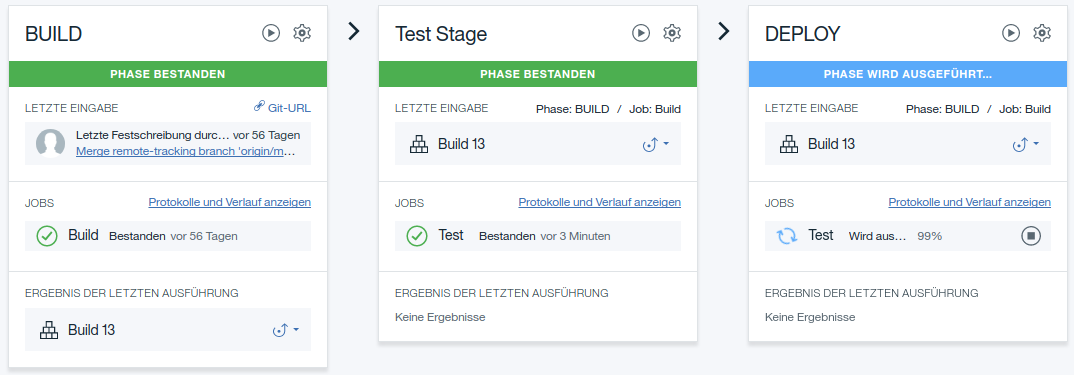
\includegraphics[scale=0.35]{images/kapitel_5/toolchain_teststage.png}
  \caption{Übersicht der Toolchain mit Test Stage}
  \label{fig:toolchain_teststage}
\end{figure}

Nach der Einrichtung wird die Test Stage nach jedem \path{push} in das zugehörige Git-Repository automatisch ausgeführt.
Im Anschluss wird die Anwendung (wie in der Abbildung zu sehen), automatisch auf das System installiert. Der komplette
Durchlauf der Toolchain sollte je nach Anzahl von Tests und Anzahl von Klassen in der Java-Anwendung wenige Minuten dauern.

Wichtig ist dabei die Reihenfolge. Im Gegensatz zum Test mit RTC (im folgenden Kapitel), wird das Backend immer getestet,
bevor es auf dem System installiert wird. Wenn ein oder mehrere Tests schiefgehen, wird auch die neue Version nicht
installiert. Dies bedeutet auch keinen Ausfall der Anwendung, wenn etwas falsch programmiert wurde.

\subsection{Mittels UCD testen}
Das Testen der Java-Anwendung mittels UCD wird in der Weboberfläche von UCD eingerichtet. Dabei wird ein neuer Task
hinzugefügt, welcher die Anwendung selbstständig testen kann.

Da der Test nicht in den Deploymentvorgang eingebaut wird, muss der Task bei Bedarf manuell gestartet werden. Es ist
sinnvoll dies immer nach einem Deployment zu tun, damit sichergestellt werden kann, dass die Anwendung korrekt funktioniert.

In Abbildung \ref{fig:ucd_teststage} auf Seite \pageref{fig:ucd_teststage} ist der eingerichtete Task mit Namen
\textit{Insurance-Backend-Interface-Integration.Test} zu sehen.

\begin{figure}[h]
  \centering
    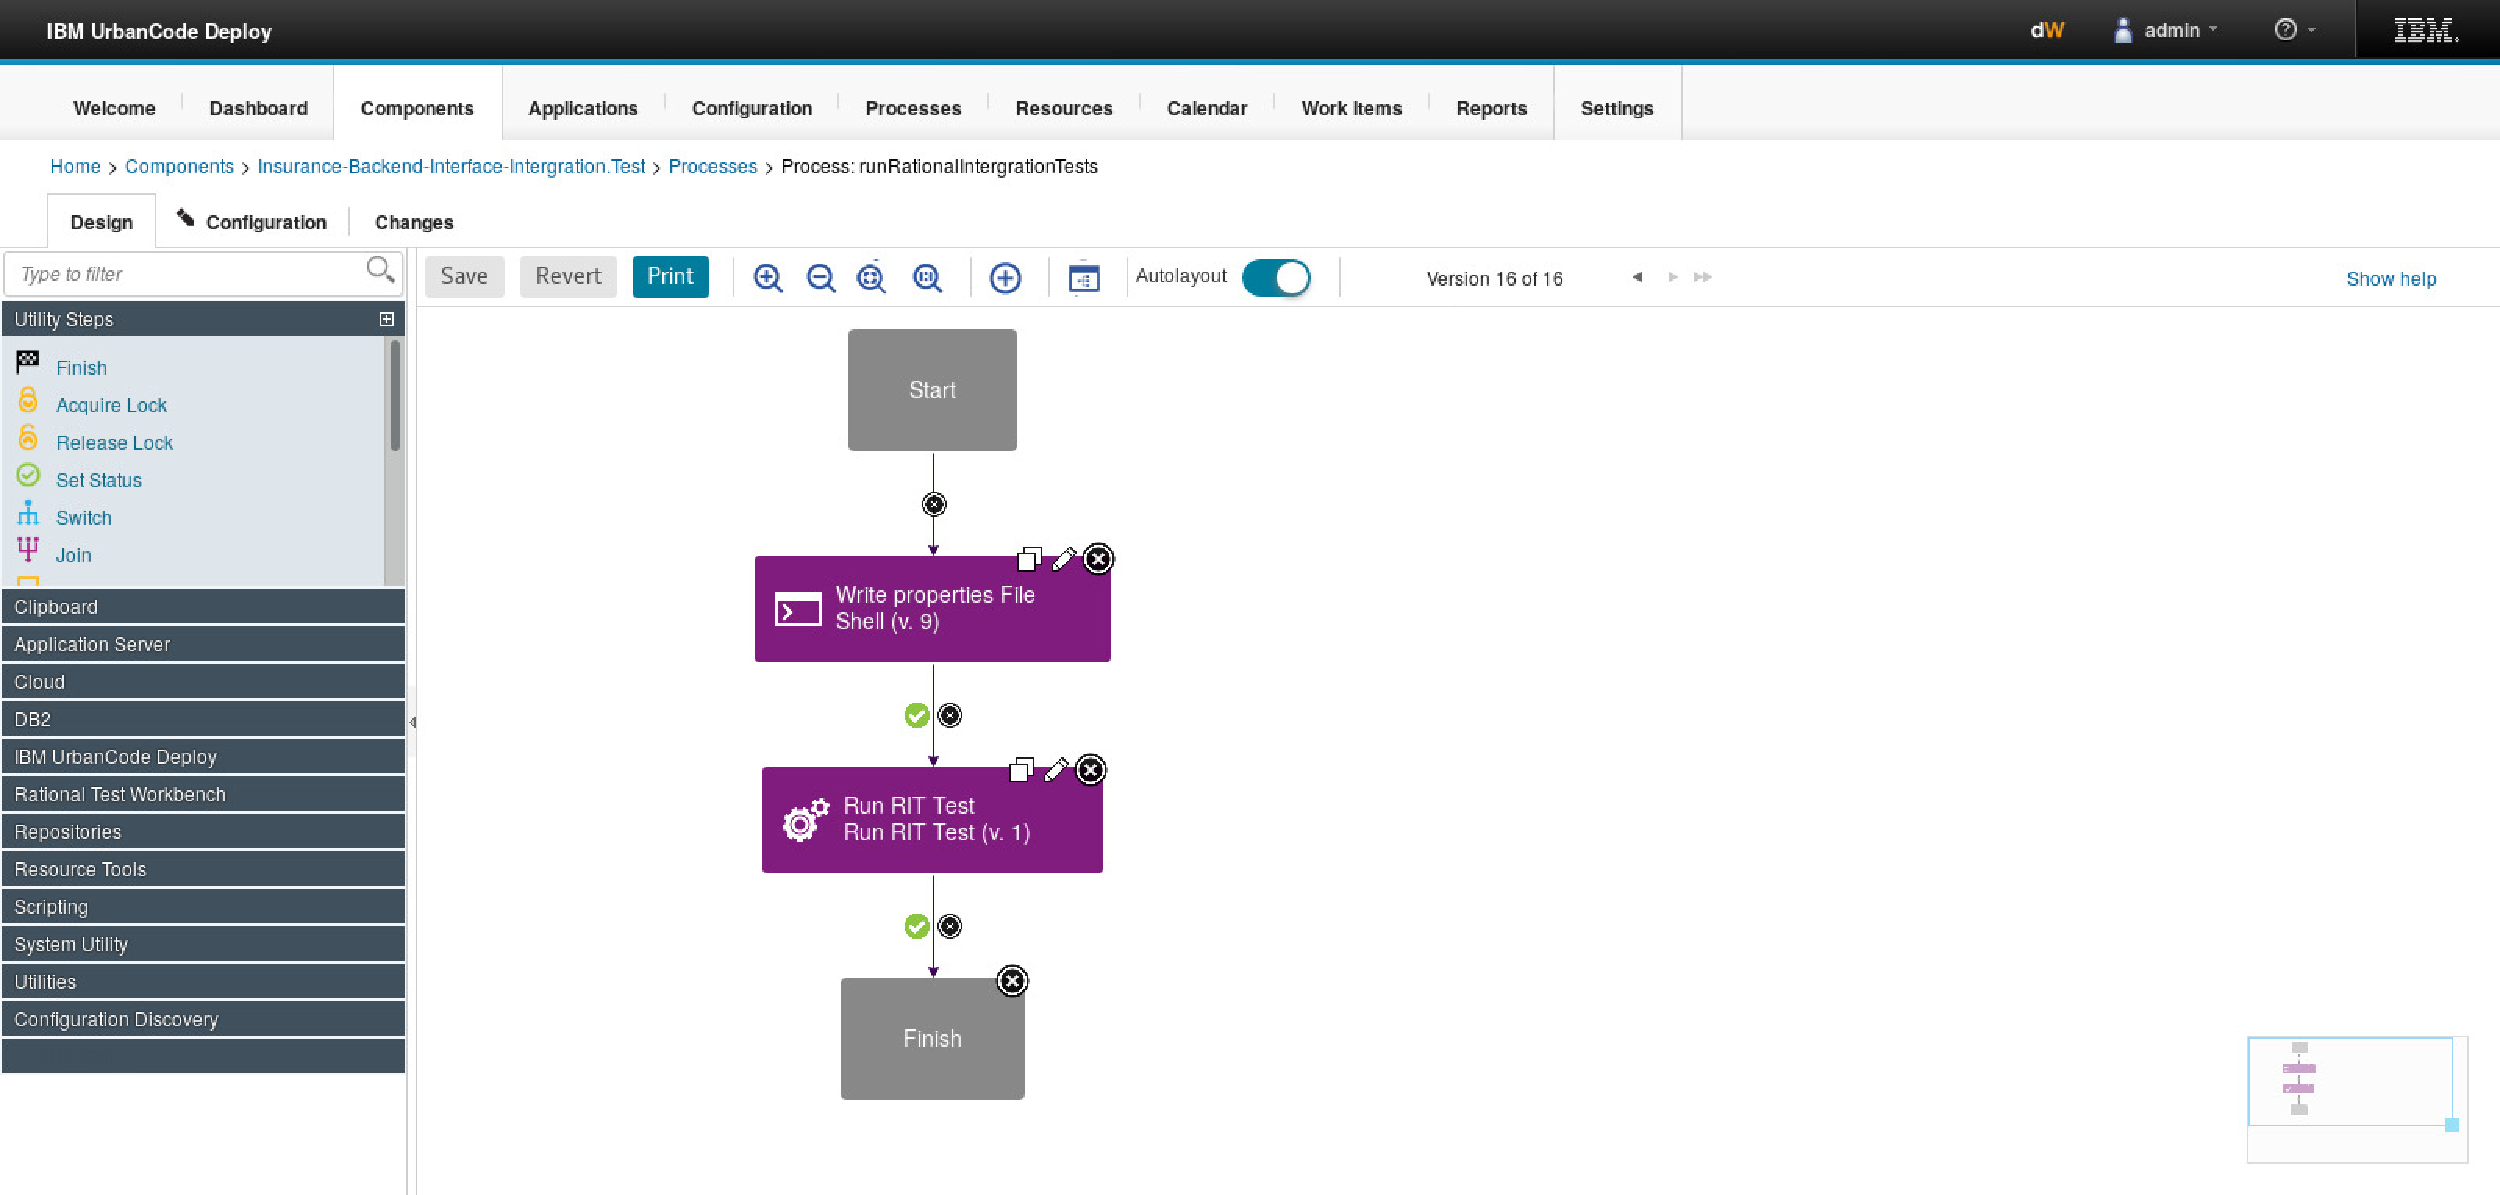
\includegraphics[scale=0.3]{images/kapitel_5/ucd_teststage.pdf}
  \caption{Übersicht des Test-Tasks in UCD}
  \label{fig:ucd_teststage}
\end{figure}

In diesem Task wird zuerst eine Konfigurations-Datei angelegt, welche vom Testscript ausgelesen wird. Bei der Konfiguration
handelt es sich um Parameter wie Speicherort der Anwendung oder verwendete CICS-Region. Dies ist wichtig, damit das
Testscript die richtige Anwendung testen kann.

Das Testscript startet ein Programm mit dem es möglich ist REST-Interfaces zu testen. Dazu wird das installierte
Java-Interface mit vordefinierten Parametern aufgerufen und die Antwort mit den geforderten verglichen. Wenn alle Aufrufe
korrekt sind, wird der Administrator benachrichtigt.

Sollte ein Test allerdings fehlschlagen wird automatisch ein \textit{rollback} eingeleitet, welcher die letzte funktionierende
Anwendung installiert. Zusätzlich wird der Administrator benachrichtigt. Dieses Vorgehen hat den Vorteil, dass eine
Anwendung die nicht richtig funktioniert bis maximal nach dem Testdurchlauf auf dem System installiert ist und keinen
größeren Schaden anrichten kann.

Nach jedem Start des Tests in UCD wird ein \textit{Execution}-Log angelegt. Dieser ist in Abbildung
\ref{fig:ucd_teststage_duration} auf Seite \pageref{fig:ucd_teststage_duration} zu sehen.

\begin{figure}[h]
  \centering
    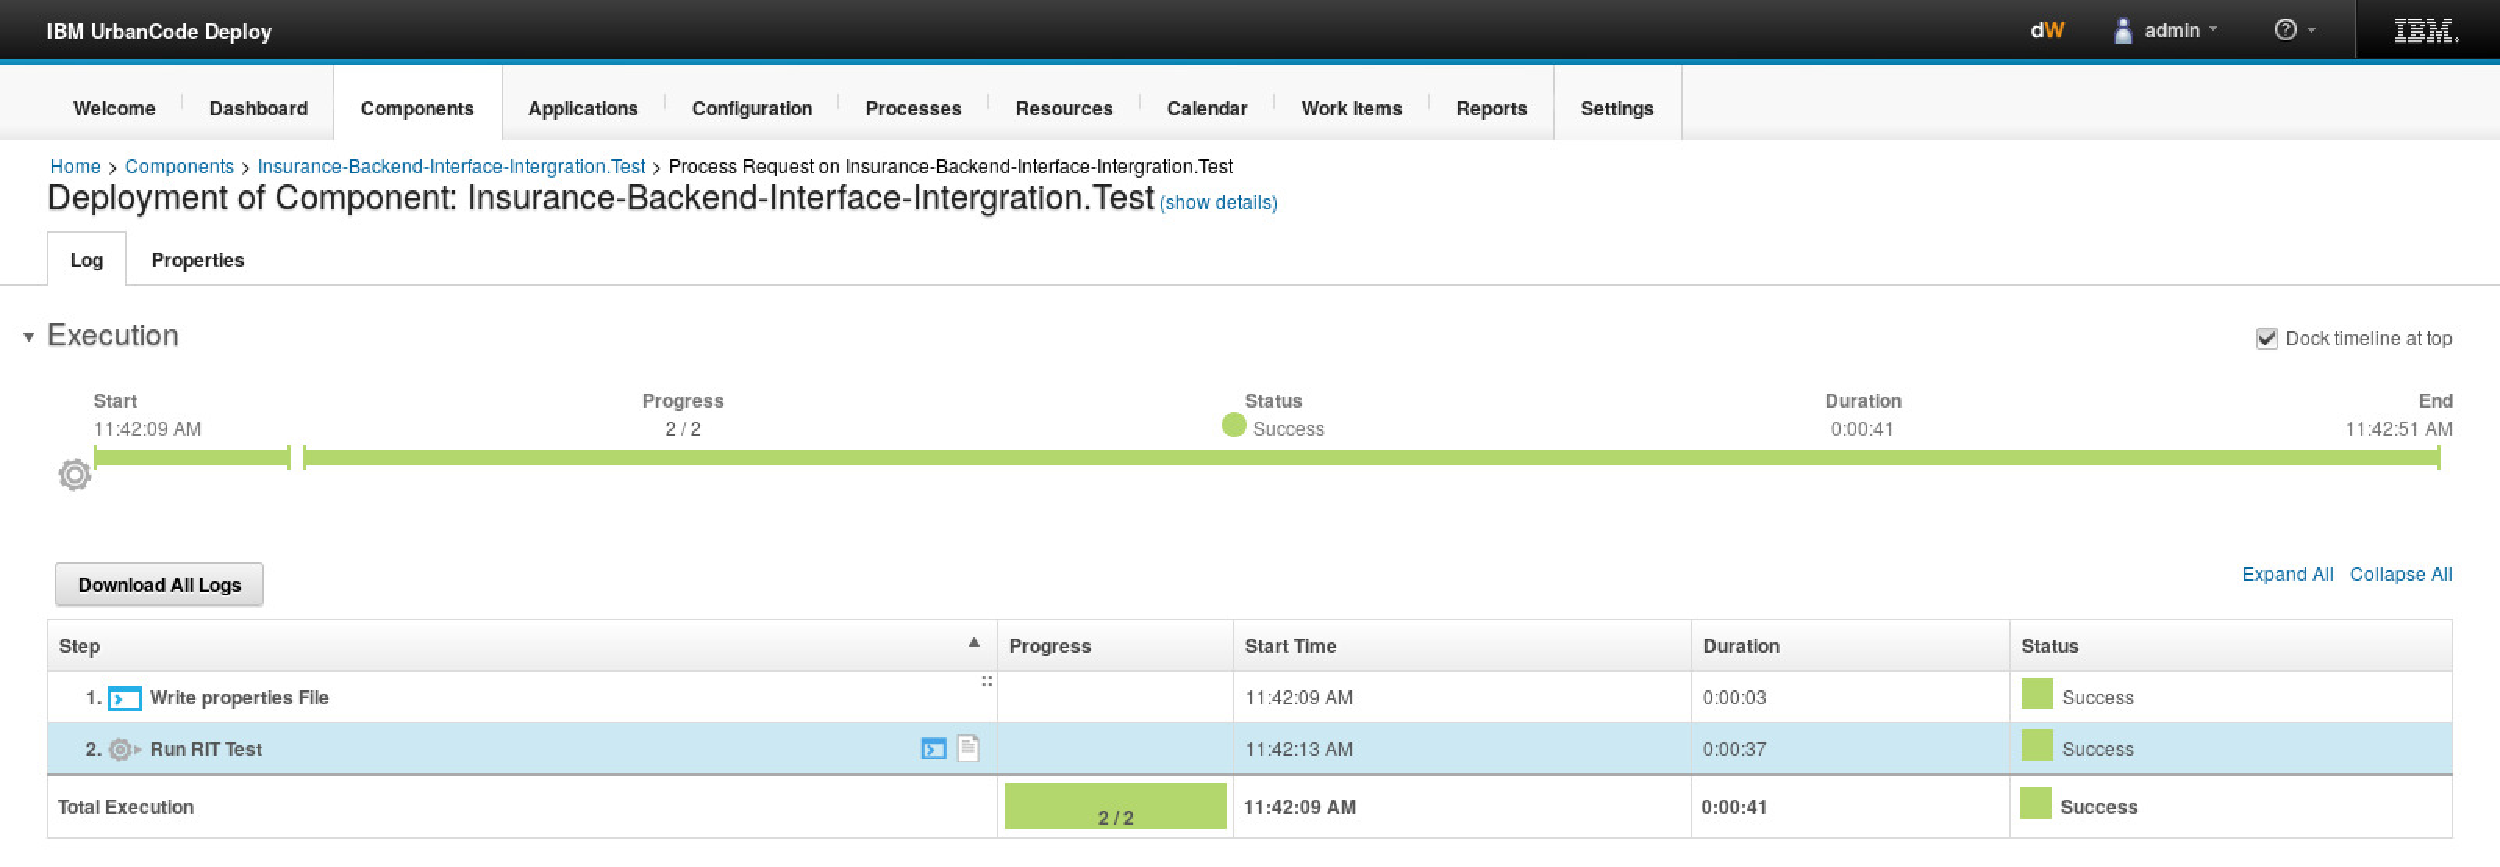
\includegraphics[scale=0.3]{images/kapitel_5/ucd_teststage_duration.pdf}
  \caption{Übersicht eines Testdurchlaufs in UCD}
  \label{fig:ucd_teststage_duration}
\end{figure}

In diesem Log kann eingesehen werden, wann der Test gestartet wurde, wie lange ein Step gebraucht hat und wie lange der
Test insgesamt gelaufen ist. In diesem Beispiel hat das Anlegen der Konfigurations-Datei nur drei Sekunden gedauert und
der komplette Test lediglich 37 Sekunden.

Insgesamt hat der Testdurchlauf im Beispiel nur 41 Sekunden gedauert und beide Steps wurden erfolgreich durchlaufen. In
einem Fehlerfall wäre im Log ersichtlich welcher Step fehlgeschlagen ist und warum.

\section{Smartphone App}
Da es sich bei den beiden Smartphone-Apps um WebView-Applikationen handelt und diese beim Start das schon betestete Web-Frontend
laden und anzeigen, decken die Frontend-Tests schon den größten Teil ab. Auch die Logik ist schon betestet.

Bei der Android- sowie bei der iOS-App gibt es allerdings wenige Zeilen Code in nativer Programmiersprache. Die
Funktion dieser muss allerdings getestet werden.

Die Tests der beiden Anwendungen werden in keinen Buildprozess eingebunden, da die Anwendungen seperat auf dem jeweiligen
Store hochgeladen oder bei Bedarf über andere Kanäle verteilt werden.

In den folgenden beiden Kapiteln wird der Aufbau der Tests genauer erklärt.

\subsection{Android-App}
Da die Android-App, genau wie das Backend, in Java geschrieben ist, werden auch hierfür die Tests in JUnit geschrieben.

Dafür wird in dem Android Studio Projekt im Verzeichnis \path{/app} in der Datei \path{build.gradle} im Bereich
\path{dependencies} die Dependency von JUnit hinzugefügt. Anschließend wird das Projekt neu gebaut, um die neue Dependency
automatisch herunter zu laden.

\begin{lstlisting}[language=bash, caption=Dependency hinzufügen, label=Dependency hinzufügen]
    androidTestCompile 'junit:junit:+'
\end{lstlisting}

Im Anschluss wird im Ordner \path{/app/src/} ein Ordner namens \path{test} hinzugefügt. In diesem werden alle Testcases
abgelegt, die ausgeführt werden sollen. Ein einfacher Test in Android sieht ähnlich einem Test in \path{Plain Java} aus.

\begin{lstlisting}[language=java, caption=Einfacher Test für Android, label=Einfacher Test für Android]
    public class ExampleUnitTest {
        @Test
        public void addition_isCorrect() throws Exception {
            assertEquals(4, 2 + 2);
        }
    }
\end{lstlisting}

Dieser statische Test prüft, ob die mathematische Gleichung \begin{math} 2+2 = 4 \end{math} zu jeder Zeit erfüllt ist.

Für die Android-Applikation ist es sinnvoll zu prüfen, ob auch die richtige URL geladen wird. Also ob das WebView-Layout
die richtige Webseite geladen hat und diese auch angezeigt wird.

Auch ist es sinnvoll während dem Test automatisiert ein Screenshot zu erstellen, welcher das Web-Frontend zeigt. So können
ggf. Fehler in der Größenanpassung behoben werden.

\subsection{iOS-App}
Für die iOS-App, welche in Swift 3 enwtickelt ist, werden die Tests in iOS Unit Testing geschrieben.

Dafür wird ein \path{Test Target} angelegt. Dies geschieht über das Hinzufügen einer \path{Unit Test Class} direkt in
XCode. Siehe dafür Abbildung \ref{fig:xcode_createtest} auf Seite \pageref{fig:xcode_createtest}.

\begin{figure}[h]
  \centering
    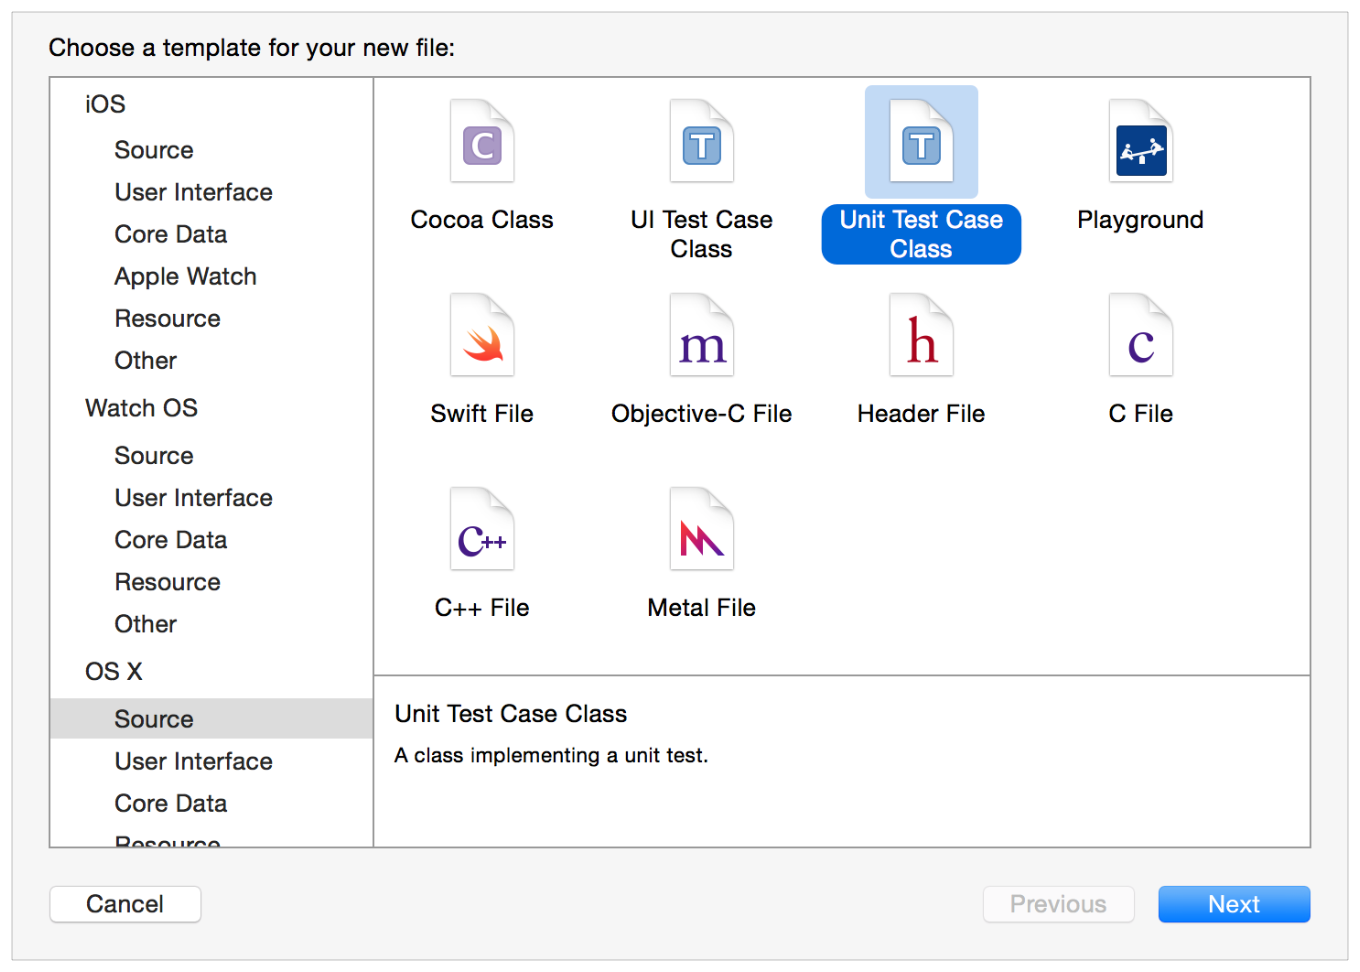
\includegraphics[scale=0.5]{images/kapitel_5/xcode_createtest.png}
  \caption{Hinzufügen einer Test Klasse in XCode}
  \label{fig:xcode_createtest}
\end{figure}

Ein beispielhafter Test kann in Listing \ref{Einfacher Test für iOS} auf Seite \pageref{Einfacher Test für iOS} eingesehen werden.

\begin{lstlisting}[language=c, caption=Einfacher Test für iOS, label=Einfacher Test für iOS]
    func testScoreIsComputed() {
      let guess = 5
      let value = 5

      XCTAssertEqual(guess, value, "Score guessed wrong")
    }
\end{lstlisting}

Dieser beispielhafte Test prüft, ob der Wert welcher geschätzt wurde (\path{guess}) gleich dem Wert ist, der fest gesetzt
wurde (\path{value}). Falls nicht, wird die definierte Fehlermeldung ausgegeben.

Wie auch in der Android-App wird hier lediglich getestet, ob das WebView-Layout die richtige Webseite lädt und auch
anzeigt. Der Rest wurde durch die Tests im Web-Frontend abgedeckt.
\chapter{Diskussion}
\label{cha:diskussion}
In diesem Kapitel werden Themen angesprochen, die bei der Arbeit mit der Hybrid-Cloud-Architektur zu beachten sind.

Auch soll auf die Sicherheit eingegangen und Use-Cases für die Architektur vorgeschlagen werden.

\section{Rechte der Entwickler}
\label{sec:rechte_der_entwickler}
In den meisten Fällen wird dem Entwickler von einem IT-Administrator die benötigte Infrastruktur oder Ressource zur
Verfügung gestellt. Das bedeutet, dass der Entwickler diese lediglich anfordern muss, sich aber keine Gedanken darüber
macht, wo die Instanz physisch läuft. Darum kümmert sich in der Regel der IT-Administrator.

In der Hybrid-Cloud ist die Idee, dass der Entwickler sich die Ressourcen die er braucht, genau wie auf einer großen
Spielwiese, allerdings selber einrichtet.

Genau in diesem Punkt liegen auch größere Probleme. Wenn der Entwickler nun Ressourcen auf dem Mainframe oder auch in der
Cloud einrichten und seine Anwendungen in beiden Netzwerken zur Verfügung stellen kann, können unter anderem
datenschutzkritische Bestandteile in der Cloud liegen, ohne dass der Entwickler das aktiv möchte.

\section{Produktion}
Für die Entwicklung einer Anwendung ist es oftmals hilfreich einen \textit{DEV}- und ein \textit{PROD}-Stage der Anwendung
bereit zu stellen. Auch kann es von Vorteil sein, mehrere DEV-Stages zu besitzen. Darauf soll im folgenden aber nicht
näher eingegangen werden, da die Erweiterung der Stages nicht sehr schwer ist.

In der \textit{DEV}-Stage werden zum Beispiel täglich Änderungen eingebaut, die dann durch die Qualitätsabteilung
getestet und mit den benötigten Anforderungen verglichen werden können.

Wohingegen in der \textit{PROD}-Stage werden neue Updates erst gebündelt installiert, wenn sie in der DEV-Stage komplett
erfolgreich getestet und mit den Anforderungen verglichen wurden.

In der Hybrid-Cloud-Architektur gibt es mehrere Möglichkeiten, diese beiden Stages abzubilden.

In der ersten Variante wird die DEV-Stage im eigenen Rechenzentrum aufgebaut und die PROD-Stage wird in der Cloud
eingerichtet. Diese Variante macht dann Sinn, wenn die Anwendung später auch in der Cloud laufen soll.

Beim Aufbau dieser Architektur, kann die Anwendung im eigenen Unternehmen getestet werden. Die Anwendung kann ggf. mit
Daten aus der eigenen Infrastruktur gefüttert werden. Wenn die Abteilung der Qualitätssicherung eine Version dann freigibt,
kann sie in der Cloud installiert werden.

Die Verbindung zwischen der Anwendung und den Daten im eigenen Rechenzentrum wird über die Hybrid-Cloud-Architektur gelöst.

Die zweite Variante sieht die DEV-Stage in der Cloud und die PROD-Stage im eigenen Rechenzentrum vor. Dies ist immer dann
sinnvoll, wenn die Anwendung später auch im eigenen Rechenzentrum laufen soll.

Der Vorteil dieses Aufbaus liegt darin, dass die Anwendung in der DEV-Stage in der Cloud getestet werden kann. Mitarbeiter
welche diese Testen, brauchen keine VPN-Verbindung ins interne Netz um auch von zu Hause testen zu können. Nachdem eine
Version freigegeben wird, wird diese auf dem internen Server installiert und steht ab sofort zur Verfügung.

Während der Testphase kann die Anwendung mit Daten aus dem Rechenzentrum über die Hybrid-Cloud versorgt werden.

Ein weiterer Vorteil ist, dass auch externe Tester für die Anwendung herangezogen werden können. Dies ist immer dann
sinnvoll, wenn Personen, die die Anwendung gar nicht kennen, einen Blick drauf werfen sollen.

\section{Use-Cases}
Für die Hybrid-Cloud-Architektur gibt es zahlreiche Use-Cases. Im folgenden soll auf ein paar wenige eingegangen werden,
welche die bedeutsamsten Use-Cases darstellen.

\subsection{Workloads}
Manchmal ist es bei der Entwicklung einer Anwendung nicht klar, wie sie im Markt ankommen wird. Ein
Cloud orientierter Ansatz folgt dem Ansatz \glqq fail fast, fail cheaply\grqq.

Danach macht es Sinn, für die Anwendung Ressourcen in der Public Cloud bereit zu stellen, die je nach Bedarf skaliert
werden können. Somit können die enstehenden Kosten überschaubar gehalten werden.

Sollte sich über die Zeit herausstellen, dass die Anwendung von den Kunden zahlreich genutzt wird, kann sie in die
bestehende Infrastruktur integirert oder eigene Ressourcen bereitgestellt werden. Für den Übergang ist es hilfreich
eine Hybrid-Cloud aufzubauen, so können Spitzenzeiten noch abgefangen werden.

\subsection{Cloud Bursting}
Das Wort \textit{Cloud Bursting} stammt aus der Situation heraus, bei der neben der eigenen Infrastruktur eine Cloud
genutzt wurde um Kapazitätsprobleme zu umgehen. Meist handelt es sich dabei um temporäre Situationen, zum Beispiel bei
einem Online-Shop während der Weihnachtszeit.

Das \textit{Cloud Bursting} wird oft mit \glqq buy the base, rent the spike\grqq~beschrieben.

Der Hybrid-Cloud-Ansatz ermöglicht es einem Unternehmen bei auftretenden und temporären Lastspitzen eine Cloud mit zu
nutzen um diese zu bewerkstelligen. Dabei wird eine sichere und schnelle Verbindung zwischen dem eigenen und den
Cloud-Ressourcen benötigt. Dies ist mit dem Secure Gateway Service möglich.

\subsection{Hochverfügbarkeit}
Eine möglichst hohe und geografisch redundante Verfügbarkeit ist durch die eigene Infrastruktur nicht immer möglich.
Gerade kleinere und mittelständische Firmen, welche nicht in jedem Kontinent ein eigenes Rechenzentrum haben, können diese
Verfügbarkeit nicht immer gewährleisten.

Durch die Hybrid-Cloud ist es möglich, dass eigene Rechenzentrum zu nutzen und nur in Ländern in denen dieses nicht zur
Verfügung steht, die Ressourcen durch die Cloud zu erweitern.

\subsection{Katastrophenwiederherstellung}
Für Unternehmen welche eine Hybrid-Cloud-Architektur nutzen ist es zum Beispiel möglich, die eigentliche Anwendung in
der Cloud laufen zu lassen und ein Backup im eigenen Rechenzentrum. So ist es möglich, wenn die Cloud-Anwendung
nicht richtig oder gar nicht funktioniert, einfach auf die im eigenen Rechenzentrum zu springen und diese weiter zu nutzen.

Alternativ kann aus dem eigenen Rechenzentrum, in dem der Quelltext der Anwendung liegt, ein neues Deployment auf die
in der Cloud liegenden Ressourcen gestartet werden, um fehlerhafte Instanzen zu elminieren.

\subsection{Rechtliche Vorgaben}
In vielen europäischen Ländern und gerade in Deutschland ist es für viele Unternehmen wichtig, dass die gespeicherten
Daten in einem Rechenzentrum gespeichert sind, welche den hohen deutschen Datenschutzrichtlinien unterliegen. Dies bedeutet
meist, dass die Daten in Deutschland gespeichert werden müssen.

Dadurch ist es nicht möglich, die komplette Infrastruktur in die Cloud zu migrieren. Durch die Hybrid-Cloud ist es allerdings
möglich den deutschen Datenschutzrichtlinien zu entsprechen in dem die Daten im eigenen Rechenzentrum verwaltet werden
und Anwendungen, welche mit den Daten arbeiten, in eine Cloud ausgelagert werden können.

So ist es zum Beispiel möglich Anwendungen für Länder zu entwickeln und dort bereit zu stellen und trotzdem mit den Daten
zu arbeiten welche sicher in Deutschland liegen. Bei solchen Anwendungen kann es sich auch um einfache
API-Management-Anwendungen handeln, welche den Traffic an den richtigen Server schicken.
\chapter{Ausblick}
\label{cha:ausblick}
In diesem Kapitel sollen weitere Services und Funktionen erwähnt werden, durch die die prototypische Anwendung erweitert
und verbessert werden kann.

Außerdem sollen Möglichkeiten aufgezeigt werden, welche die Arbeit mit der Hybrid-Cloud-Architektur unter Bluemix
und z Systems vereinfacht.

\section{Nutzen von API-Connect}
In der jetzigen Version wird um die COBOL-Anwendung ein Java-Wrapper geschrieben, welcher ein REST-Interface für Anfragen
von außen zur Verfügung stellt. Wenn die COBOL-Anwendung erweitert werden würde oder noch andere Funktionen dieser genutzt
werden sollen, muss immer die Java-Applikation angepasst werden.

Alternativ ist es möglich, den API-Connect Service von Bluemix zu nutzen, welcher eine browserbasierte GUI zur Verfügung
stellt, mit welcher es möglich ist, REST(Ful)-Interfaces zu entwickeln.

Bei der Nutzung des Services würde das Web-Frontend (und die Smartphone-Apps) ihre Anfragen an den Service schicken. Dieser
würde dann über den Secure Gateway eine Verbindung auf die COBOL-Anwendung aufbauen und Informationen abrufen.

Außerdem ist es möglich, dass der API-Connect Service auch den DB2 REST Service aufrufen kann. So hat das Web-Frontend
lediglich eine Schnittstelle, die es ansprechen muss. Der API-Connect Service schickt die Anfragen dann an verschiedene
Anwendungen weiter.

\section{Open Service Broker Projekt}
Da die Schnittstellen eines Servcie Brokers von der \textit{Open Service Broker Projekt} Organisation definiert werden und
dieser zahlreiche große Firmen angehören, welche jeweils eigene Cloud-Lösungen anbieten, kann der entwickelte Service
Broker auch auf anderen Cloud-Infrastrukturen eingerichtet werden.

So könnte der Service Broker zum Beispiel auch bei Amazons AWS instanziiert werden und somit theoretisch eine Verbindung
zwischen dieser Cloud und einer anderen Cloud oder einem Mainframe aufgebaut werden. Allerdings unterstützt AWS bislang
nicht die Möglichkeit VPN Verbindungen zu anderen Netzwerken aufzubauen.

\section{Einbindung in den Katalog}
Aktuell ist der entwickelte Service Broker nur in der Bluemix Organisation über die Cloud Foundry CLI sichtbar in der er
eingerichtet wurde. Dort auch nur für Nutzer, welche auf die Organisation Zugriff haben. Er erscheint jedoch nicht im
Bluemix Katalog.

Das Hinzufügen eines Service Brokers in den allgemeinen Bluemix Katalog kann lediglich durch einen Administrator erfolgen.
Dieser kann allerdings einstellen, in welcher Region oder welchen Kundengruppen dieser Service Broker zur Verfügung stehen
soll.

Beim Entwickeln des Service Brokers wurde dieser schon mit einem Icon und einem Beschreibungstext ergänzt, sodass das
Hinzufügen in den Katalog keine Nacharbeit am Quellcode des Service Brokers bedeuten würde.

Nach weiteren Tests könnte eine Anfrage an einen Administrator von Bluemix Public gestellt werden, sodass der Service
Broker in den Katalog aufgenommen werden kann. Dies geschieht über das
Support-Formular\footnote{https://developer.ibm.com/answers/questions/ask/?topics=bluemix}.

\section{Weitere zOSMF Interface Funktionen}
Bisher wird im Service Broker neben dem Abruf der allgemeinen Informationen lediglich noch die Funktion zum Ausführen
von Workflows und Jobs der einzelnen Instanzen des zOSMF Interfaces genutzt.

Das Interface von zOSMF bietet allerdings noch weitaus mehr Funktionen.

Eine Möglichkeit wäre das Auslesen der aktuellen Workflows. Aktuell kann lediglich ein Workflow gestartet werden,
welcher eine CICS-Region erstellt. Wenn alle Workflows dynamisch abgefragt werden, könnten neu erstellte auch ausgeführt
werden.

Desweiteren könnten Workflows in Bluemix mit einem visuellen Editor geschrieben werden (ähnlich
Node-Red\footnote{https://nodered.org}) und dann an zOSMF übertragen werden. So könnten, auch automatisiert, neue Workflows
entstehen, welche Runtimes oder Anwendungen auf dem Mainframe erstellen.

Auch könnten die Notifications für einen Benutzer ausgelesen werden. Dadurch wäre es möglich festzustellen, wann der
gestartete Workflow abgeschlossen wurde. Denn immer wenn ein Workflow gestartet, gestoppt, durchgeführt oder in einen
Fehler läuft, wird der Benutzer mit einer Notifications darauf aufmerksam gemacht.

\section{MobileFirst Platform}
Bei den Smartphone-Apps handelt es sich jeweils um native Applikationen, welche ein WebView-Layout beinhalten, in das beim
Start immer die aktuellste Version des Web-Frontends geladen wird.

Die Interaktion mit dem Frontend übernimmt das WebView-Layout, und getätigte Einstellungen werden auf dem Smartphone
persistiert.

Um die MobileFirst Platform zu nutzen, muss der Service in das Web-Frontend eingebunden werden. Die MobileFirst Platform
nutzt dabei Cordova um die Webseite dann in eine native Android, iOS und Windows App zu kompilieren. Dabei werden
HTML Elemente durch die Systemeigenen ersetzt. Ein HTML-Button wird dann zum Beispiel zu einem nativen Button.

Der große Vorteil der Nutzung dieser Platform ist neben der Möglichkeit neben Android und iOS auch Windows Phone zu
unterstützen, dass weiterhin nur ein Web-Frontend geschrieben werden muss und dies dann in eine native Applikation
umgewandelt werden kann. Daraus ergibt sich ein besseres \textit{Look and Feel} und eine höhere Performance
der Applikation.

\section{Native Smartphone-Apps}
Anstatt wie bisher das Web-Frontend in einen WebView-Layout zu laden oder mit Hilfe der MobileFirst Platform native Applikationen
aus HTML zu erstellen, können für die verschiedenen Smartphonebetriebssysteme jeweils eigene, native App geschrieben
werden.

Dies hat, neben vielen weiteren, den Vorteil, dass direkt auf die Hardware des Systems zugegriffen werden kann und Daten
mit anderen Apps ausgetauscht werden können.

So ist es zum Beispiel möglich, Informationen, die in der Anwendung angezeigt werden, mit den Kontaktdaten auf dem Smartphone
abzugleichen und den Datenstand gegenseitig anzupassen.

\section{Erweiterung der Toolchain}
\label{sec:erweiterung_der_toolchain}
Die in diesem Projekt genutzte Toolchain besitzt lediglich eine rudimentäre Verbindung zum Mainframe um dort eine Anwendung
einzurichten. Diese wurde händisch über das FTP-Protokoll aufgebaut. Allerdings gibt es auch für die Toolchain möglichkeiten
eigene Services zu schreiben. Ähnlich dem Service zur Integration eines GitHub Projektes.

Die Funktion der Toolchain könnte dahingehend erweitert werden, dass aus dem instanziierten Secure Gateway Service alle
Verbindungen zu den CICS-Regionen herausgesucht werden und automatisch ein Build-Prozess für diese eingerichtet werden kann.

Somit wäre ein deployment auf die verschiedenen CICS-Regionen einfacher über die Toolchain möglich ohne für jede CICS-Region
selbstständig eine FTP- oder SSH-Verbindung aufzubauen.

\section{Automatischer Secure Gateway}
Wenn über den Service Broker eine neue CICS-Region erstellt wird und diese auch über die Cloud genutzt werden soll, muss
nach der erfolgreichen Einrichtung händisch ein Ziel im Secure Gateway Service hinzugefügt werden.

Einfacher wäre es, wenn es bei der Erstellung einer CICS-Region eine Auswahl mit \textit{Make public} gäbe, welche nach
Auswahl ein Ziel automatisiert hinzufügt.

Um diese Funktionalität zu erreichen, muss der Secure Gateway Service in Bluemix überarbeitet werden. Er muss über ein
REST-Interface verfügen, über das es möglich ist, neue Ziele hinzuzufügen. Als Parameter müsste das Interface zumindest
\textit{Name}, \textit{IP-Adresse} und \textit{Port} unterstützen.

\section{Auslesen der zOSMF-URL}
Um die Hybrid-Cloud-Architektur zu nutzen, muss ein Ziel im Secure Gateway zum zOSMF erstellt werden. Anschließend kann
der Service Broker instanziiert werden. Dieser muss im ersten Schritt mit URL, Benutzername und Passwort für zOSMF
eingerichtet werden.

Einfacher wäre es, wenn die angelegte zOSMF-URL im Secure Gateway Service automatisiert vom Service Broker ausgelesen
werden könnte. Um dies zu realisieren, muss der Secure Gateway Service über ein REST-Interface verfügen, über den alle
eingerichteten URLs ausgelesen werden können.

Anschließend könnte der Service Broker entweder alle URLs anzeigen und der Benutzer wählt die Richtige aus, oder anhand
der Benamung der URL wird dieser vorausgewählt. Denkbar wäre die Benamung \path{zOSMF}.

\section{Automatisches Auslesen von URLs}
Damit das Frontend mit dem Backend auf dem Mainframe kommunizieren kann, muss in Bluemix im Secure Gateway Service ein
Ziel dafür eingerichtet werden. Diese URL muss im Frontend gespeichert werden, damit die Angular-Factories Anfragen an
das Backend schicken können.

Für die Umsetzung wäre es einfacher, wenn der Secure Gateway Service über die VCAP-Variablen alle seine Ziele
zur Verfügung stellen würde. So könnte das Frontend die URL dynamisch aus dem Secure Gateway Service auslesen und die
Anfragen an das Backend schicken.

Ein weiterer Vorteil wäre, dass wenn sich zum Beispiel die CICS-Region ändert eine neue URL hinzugefügt werden kann und
das Web-Frontend automatisch über den Namen das richtige Ziel auswählt ohne ein neues Deployment mit Quellcodanpassungen
durchführen zu müssen.

Auch wäre es so einfacher eine \textit{DEV}- und \textit{PROD}-Stage des Web-Frontend zu nutzen. Entsprechend wären zwei
Ziele im Secure Gateway Service eingerichtet (welche zum Beispiel auf unterschiedliche CICS-Regionen zeigen), und das
Web-Frontend wählt, je nach Stage, die richtige URL aus.

\section{Unterschiedliche Mainframes}
Aktuell wird für jede Konfiguration eines Mainframes ein eigenständiger Service Broker benötigt. Meist unterhält ein
Unternehmen aber mehrere z Systems in seinem Rechenzentrum.

Sinnvoll wäre, dass der Service Broker mehrere Verbindungen zu unterschiedlichen z Systems aufbauen kann (vorausgesetzt
den Verbindungen durch den Secure Gateway Service). Dann könnte bei der Erstellung einer CICS-Region nach dem z System
gefragt werden, auf dem die CICS-Region eingerichtet werden soll.

Auch könnten die \textit{Tenants} für die Auswahl der verschiedenen z Systems genutzt werden.

\section{Fragenkatalog}
Wie in Kapitel \ref{sec:rechte_der_entwickler} auf Seite \pageref{sec:rechte_der_entwickler} beschrieben, müssen dem
Entwickler Hilfen angeboten werden, um sicherzustellen, dass die datenkritischen Anwendungen richtig geschützt werden
können.

Dafür wäre bei der Erstellung einer neuen CICS-Region über den Service Broker ein vorangeschalteter Fragenkatalog hilfreich.
In diesem wird der Benutzer gefragt, um welche Art von Anwendung es sich handelt und um welche Daten es geht. Nach der
Beantwortung der Fragen, kann der Service Broker die Rechenpower in Form einer CICS-Region auf dem Mainframe oder
als zum Beispiel Cloud Foundry Applikation in Bluemix zur Verfügung stellen.

Die Entscheidung, wo die Ressourcen bereit stehen, trifft also nicht der Entwickler sondern der Service Broker.

\section{Hinzufügen einer Applikation}
Bei der Einrichtung einer CICS-Region wird der hinterlegte Workflow genutzt, um den Job durchzuführen. Dabei ist fest
vorgegeben, wie und mit welchem Inhalt die CICS-Region erstellt wird. Ein Abändern des Workflows ist oft mühsam und
setzt technisches Verständnis voraus.

Da CICS-Regionen ohne vorinstallierte Anwendung wenig Sinn machen, könnte bei der Erstellung einer solchen auch gleich
nach einer Anwendung gefragt werden, welche vorinstalliert werden soll. Die Auswahl der Anwendungen könnte aus dem RTC bzw.
UCD kommen (eine Verbindung dazu gibt es schon). Dort könnten alle Verfügbaren Anwendungen ausgelesen und dem  Benutzer
via Auswahl angezeigt werden.

Im nächsten Schritt würde die CICS-Region erstellt werden und im Anschluss über UCD ein Build auf dieses System mit der
ausgewählten Applikation.

\section{Andere Cloudanbieter}
Zur Zeit kann der Service Broker lediglich CICS-Regionen über zOSMF auf einem Mainframe bereitstellen. Oftmals gibt es
in einem Unternehmen neben einem Mainframe auch mehrere Cloudanbieter. Denkbar wäre die Integration eines anderen
Cloudanbieters.

So hätte der Nutzer des Bluemix Service Brokers die Möglichkeit neben dem Erstellen einer CICS-Region auf dem Mainframe
auch das Hinzufügen von Runtimes in anderen Cloud-Umgebungen um eine Anwendung über mehrere Cloud-Anbieter und seinem
Mainframe hinweg zu entwickeln.

Dafür müsste lediglich eine Verbindung zum weiteren Cloud-Anbieter hergestellt werden und dem Service Broker der dortige
Benutzername mit Passwort bekannt gemacht werden.
\chapter{Zusammenfassung}
\label{cha:zusammenfassung}

Im Rahmen dieser Arbeit wurde eine Hybrid-Cloud-Architektur entwickelt und diese anschließend durch eine prototypische
Implementierung realisiert. Ziel war es, einem Unternehmen dabei zu helfen, die Vorzüge einer Cloud zu nutzen, ohne auf
die eigene Infrastruktur verzichten zu müssen.

Gerade die Idee hinter einer serviceorientierten Architektur, Programme auf verschiedenen Systemen zu einer Gesamtanwendung
zu verbinden, kann durch die Hybrid-Cloud realisiert werden. Dabei läuft ein Teil der Anwendung auf einem
internen Mainframe und ein anderer Teil kann öffentlich in der Cloud aufrufbar sein.

Basis für die Architektur bildet ein z Systems und Bluemix, die Cloudumsetzung der IBM. Die Wahl fiel zugunsten
dieses Toolsets aus, da die Komponenten sehr weit verbreitet sind und viele offene Standards besitzen.

Am Anfang der Arbeit wurde die Hybrid-Cloud-Architektur entwickelt und im weiteren Verlauf umgesetzt. Die verwendeten
Zusatzprogramme wie z.B. Runtimes wurden mit anderen verglichen und anschließend installiert und eingerichtet.

Nachdem die Architektur aufgebaut war, wurde sie mittels einer prototypischen Implementierung umgesetzt. Teil der Umsetzung
war ein Web-Frontend auf Basis von AngularJS und Material Design sowie zwei Smartphone-Applikationen.

Aus den Erfahrungen, die in der Entwicklung der Architektur und der prototypischen Anwendung gesammelt wurden, ergaben
sich Diskussionsthemen und einige Erkenntnisse, die der Weiterentwicklung des Systems dienen können. Diese wurden in
Kapitel \ref{cha:ausblick} ausgeführt.

Letztendlich bleibt mir zu sagen, dass sich die Hybrid-Cloud, im Gegensatz zur reinen Cloud, in Europa und insbesondere
in Deutschland durchsetzen wird. Der einfache Grundaufbau, die vielseitige Konfiguration und die zahlreichen
Einsatzmöglichkeiten tun ihr Übriges dazu.

Das Fazit der IBM Studie \textit{Tailoring hybrid cloud: Designing the right mix for innovation, efficiency and growth}
besagt abschließend, \glqq [\ldots] dass 80 Prozent der Unternehmen weltweit die Cloud bereits nutzen und zwar meist in
hybrider Form [\ldots]\grqq~\cite{online_ausblick_fazit}.

% Alle Einträge der BibTeX Datenbank "zitieren"
\nocite{*}
% Einstellen des Bibliography-Stils für das Literaturverzeichnis
\bibliographystyle{abbrvdin}
% Auswahl der BibTeX Datenbank für das Literaturverzeichnis
\bibliography{literatur}

% Abbildungsverzeichnis ausgeben
\listoffigures

% Tabellenverzeichnis ausgeben
%\listoftables

% Das Listings-Verzeichnis scheint mit manchen Versionen vom Koma-Script
% bzw. des Listings Pakets nicht ohne weiteres zu funktionieren
\lstlistoflistings

% Anhang beginnen (Formatierung umschalten)
\appendix
\chapter{Anhang}
\label{cha:anhang}

\section{Datenbankschema}
\label{anhang:datenbankschema}

\begin{figure}[h]
 \centering
   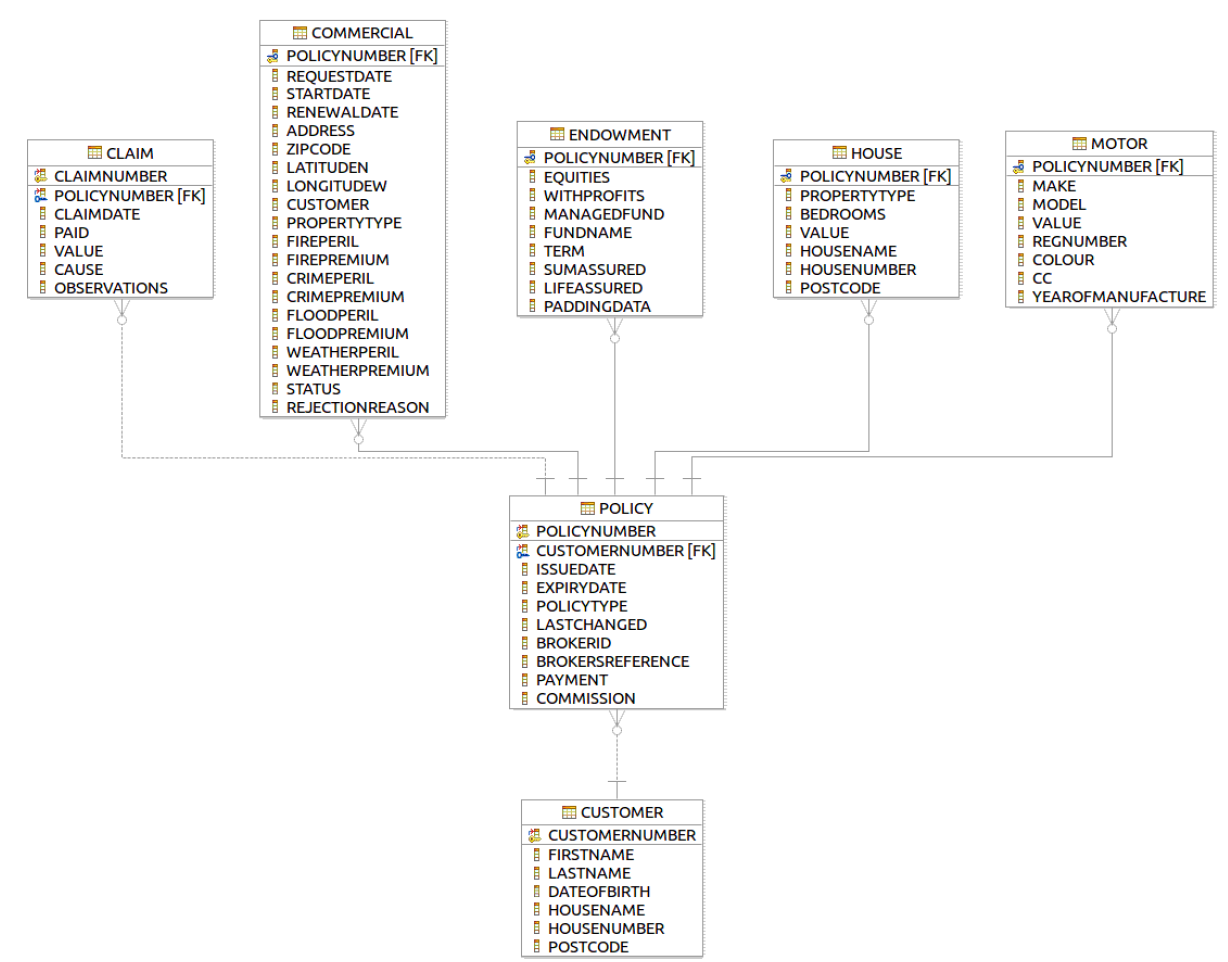
\includegraphics[scale=0.4]{images/anhang/datenbank.png}
 \caption{Schema der GenApp-Datenbank}
\end{figure}

\newpage

\section{Flow Chart}
\label{anhang:flowchart}

\begin{figure}[h]
 \centering
   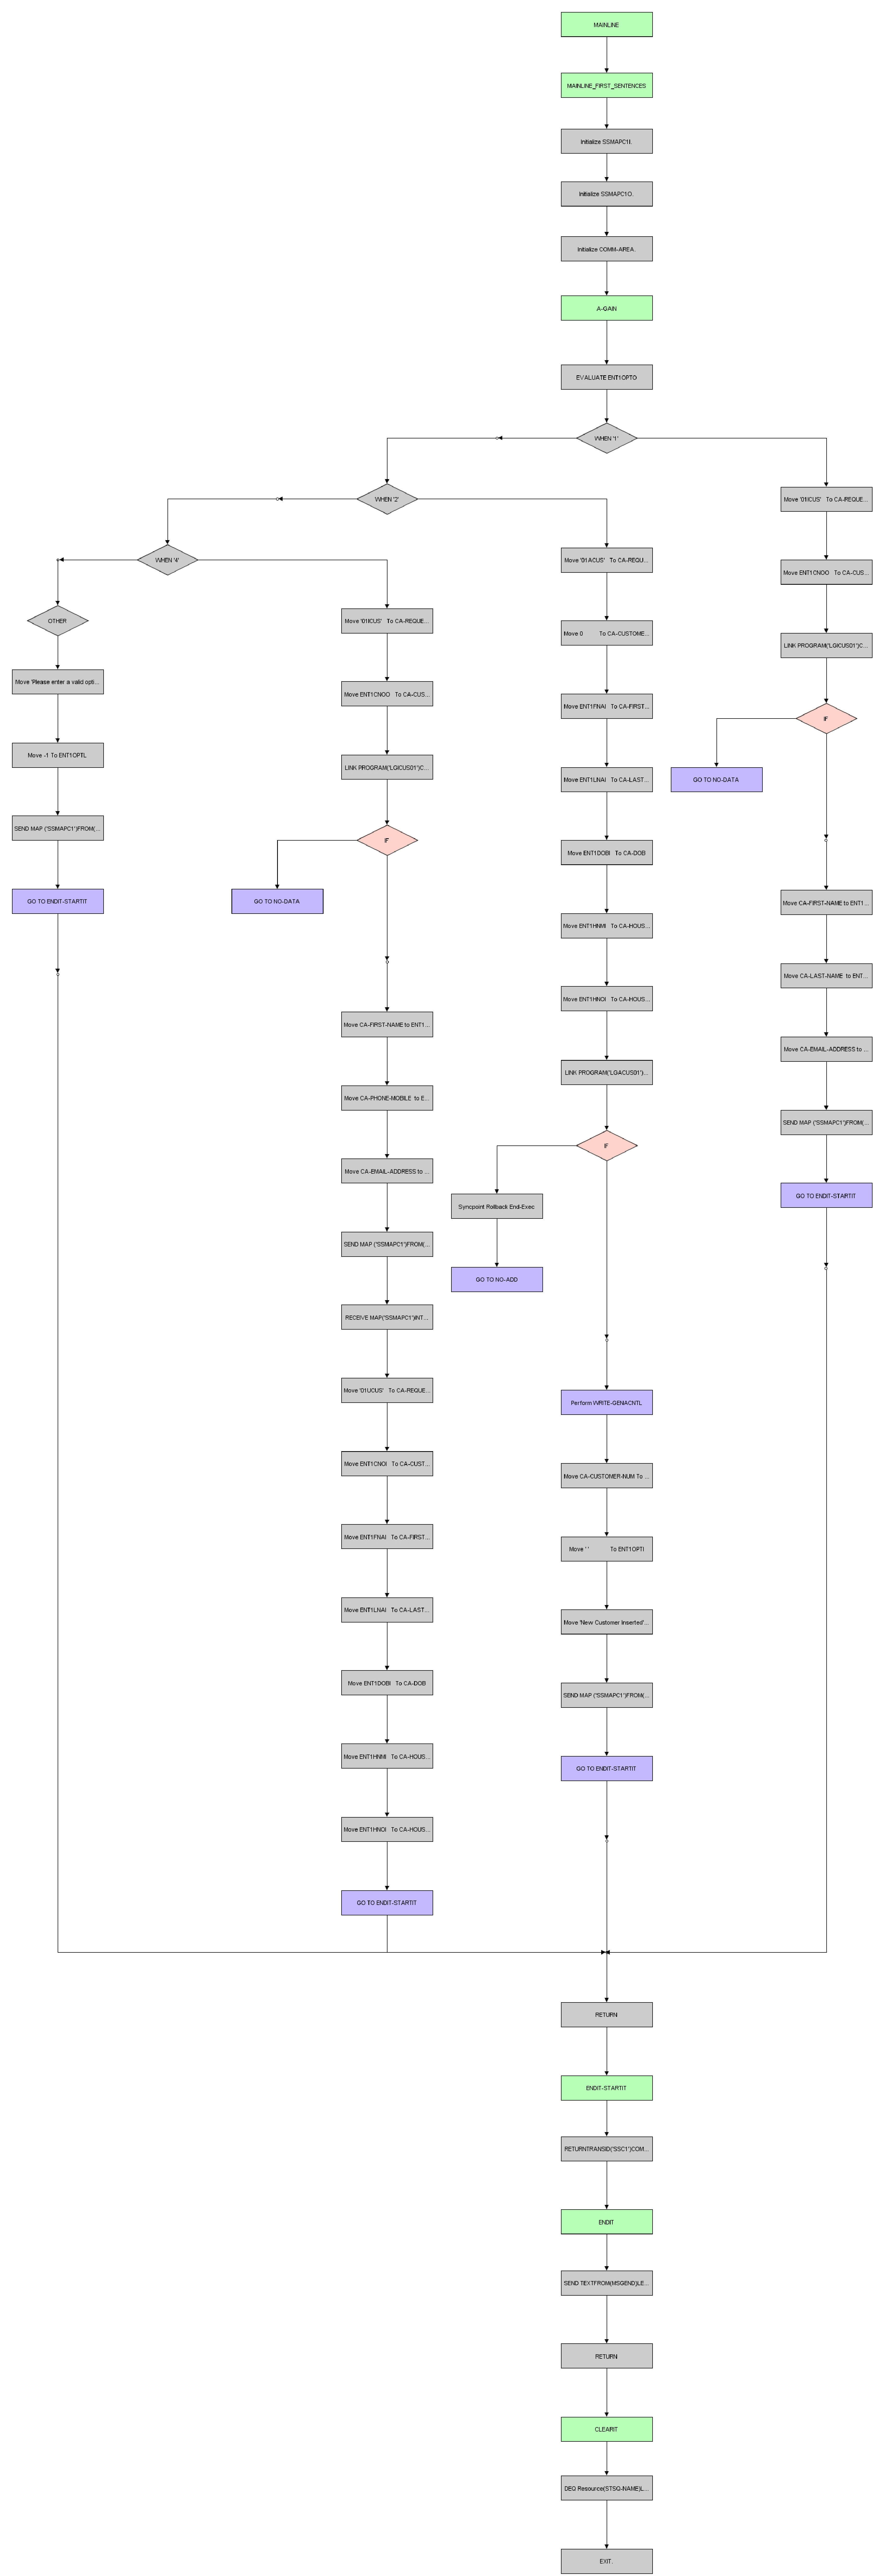
\includegraphics[scale=0.097]{images/anhang/ibmad_flowChart.pdf}
\end{figure}

% Ausgabe des Wortindex
% idxtotoc Option scheint nicht zu funktionieren
%\clearpage
%\addcontentsline{toc}{chapter}{Index}
%\printindex

\end{document}
